% !TEX root = ../partial-sdm.tex

Performance matters. A framework that does not offer cutting-edge performance is not valuable.  If an experiment takes a few seconds, there is no point arguing whether we should try it. If it takes a few hours, maybe we should think first. If it takes a few days --- or more ---, it is important to devise a good plan.  As SDM consumes large processor and memory resources, some experiments may take a long time.

Each scan on a 1,000-bits SDM with 1,000,000 hard locations executes $10^9$ bit compares through $10^9/64 = 15,625,000$ XORs and calls to the built-in popcount. So, 10,000 writes execute $10^{13}$ bit compares, while a 6-iterative reading executes $6 \cdot 10^{12}$ bit compares. The heatmap of Figure \ref{fig:cir-dist-10k-writes-kanerva} executed $3.05 \cdot 10^{15}$ bit compares. For comparison, the number of seconds since Jesus's birth is 63,639,648,000 = $6.36 \cdot 10^{10}$. The number of people who have ever lived on earth is estimated to be $1,08 \cdot 10^{11}$. There are approximately $1.8 \cdot 10^{9}$ websites on the internet. A modern laptop can increment a counter $5 \cdot 10^{8}$ times per second. Hence, a naive implementation of SDM may take several hours --- or days --- to simply write 10,000 random bitstrings.

Amazon EC2 p3.2xlarge has generated the heatmap of Figure \ref{fig:cir-dist-10k-writes-kanerva} in 15 minutes and 3 seconds. It has compared $3.37 \cdot 10^{12}$ bits per second through $52.6 \cdot 10^{9} = 52.6 \text{ billion}$ XORs and popcounts per second. It is a 60-fold improvement over the first versions of the code which took 16 hours to generate the same heatmap (and its memory use was already optimized and the computations were distributed in threads).

We have created a benchmark to be able to compare the performance of different devices. So, the same performance test was executable in our devices, with results reported in tables and figures. The benchmark has 3 parts: (i) the first part consists of comparing the available OpenCL kernels to find which works best for that device; than (ii) the second part consists of comparing the linear scanner, the thread scanner, and the OpenCL scanners with the best kernel found in part one; finally, (iii) the third part consists of comparing read and write operations using the thread scanner and the OpenCL scanner with the best kernel. Each part was run for three SDM setups: (i) $n=1,000$, $r=451$, and $H=1,000,000$; (ii) $n=256$, $r=103$, and $H=1,000,000$; and (iii) $n=10,000$, $r=4850$, and $H=1,000,000$. The whole source code is available in the ``Performance test'' notebook \citep{sdmframework}. We would like to invite the reader to run this benchmark and, if possible, share the results.

Our first device was a personal MacBook Pro Retina 13-inch Late 2013 with a 2.6GHz Intel core i5 processor, 6GB DDR3 RAM, and Intel Iris GPU. It was not possible to run the 10,000-bits on this device because there was no memory available --- it needs 37.25 GB of memory. For its results, see Table \ref{tab:perf-macbook}

Our second device was an iMac Retina 5K 27-inch 2017 with a 3.8GHz Intel core i5 processor, 8GB DDR4 RAM, and a Radeon Pro 580 8G CPU. For its results, see Table \ref{tab:perf-imac}.

Beyond that, we were also running in state-of-the-art devices: (i) an Amazon EC2 p2.xlarge with Intel Xeon E5-2686v4 processor, 61GB DDR3 RAM, and NVIDIA K80 GPU (see Table \ref{tab:perf-ec2-p2}), and (ii) an Amazon EC2 p3.2xlarge with Intel Xeon E5-2686v4 processor, 488GB DDR3 RAM, and NVIDIA Tesla V100 GPU (see Table \ref{tab:perf-ec2-p3}).


\section{Kernels comparison}

OpenCL is a framework for writing software that executes in \emph{heterogeneous} devices \citep{munshi2009opencl}, like CPUs, GPUs, FPGA and other co-processors for hardware acceleration. Because they are heterogeneous, they may differ a lot in architecture and performance, which means there is no one-size-fits-all kernel. A \emph{kernel} is generally a small function on the code that runs in thousands of parallel threads, executing the same steps on different parts of a large vector or matrix. The slower kernel for one device may be the fastest for another device, as we will see happening in our case.

A total of 8 kernels have been developed for benchmarking in our framework: single\_scan0, single\_scan1, single\_scan2, single\_scan3, single\_scan4, single\_scan5, single\_scan5\_unroll, and single\_scan6. Each scan uses a different algorithm to do exactly the same thing: calculate which hard locations are inside the circle of the given bitstring. They differ in how they split the work between work-groups and how they explore the GPU architecture to obtain performance gains.

The difference in which kernel is the best also depends on the SDM setup. The best kernel for the 1,000-bits SDM in the iMac 2017 was single\_scan5\_unroll with average scan time of 3.61ms; but, for the 256-bits SDM in the same device, it was single\_scan0 with average scan time of 3.03ms; while, for the 10,000-bits SDM in the same device, it was single\_scan6 with 10.96ms (see Table \ref{tab:perf-imac}).

We recommend users to run a specific kernel comparison test for their own GPU and SDM settings.  This is available in the Jupyter notebooks.


\section{Scanners comparison}

In this section, we are comparing the OpenCL scanner (with the best kernel) with the linear scanner and the threads scanner. Again, which one is faster depends on the SDM settings. In the iMac 2017, the fastest scanner for a 1,000-bits SDM was the OpenCL scanner with \lstinline{single_scan5_unroll}, but, for a 256-bit SDM, it was the threads scanner.

What happened here is that the OpenCL kernel chosen was a generic one which performs the scan for any SDM. It is always possible to optimize the OpenCL kernel to a specific setting, and it would be faster than the threads. By default, the framework chooses a generic kernel which we believe would be reasonable for the most common setups.
% TODO Run the optimized kernel and show the results.

We can notice that Amazon EC2 p3.2xlarge and p2.xlarge's linear and thread scanners, both running on CPU, were much slower than the CPU of both the personal MacBook Pro and the iMac 2017. As Amazon EC2 are virtual machines with GPU devices, their CPU is shared with other virtual machines which significantly reduces CPU power. Hence, for both virtual machines we have tested, using the GPU seriously boosts performance, but using the CPU should be avoided (see Table \ref{tab:perf-imac})

\section{Read and write operations}

Even though scanning is an important part of the operations, we are really interested in the performance of the entirety of operations themselves. Comparing the times of the thread and OpenCL scanners with the times of their respective operations (either read or write), we can notice that their difference remains almost constant, which means the operation time itself is negligible when compared to the scan time. In other words, in order to gain even more performance, we have to pursue ways to improve the scan.


\begin{table}[!htb]
\centering
\begin{tabular}{lrrrr}
    \toprule
    & \textbf{256 bits} & \textbf{1,000 bits} & \textbf{10,000 bits} \\ \hline
    \hline
	Kernel & Duration (ms) & Duration (ms) & Duration (ms) \\ \hline
    single\_scan0 &  8.36 & 23.60 &  \\
    single\_scan1 & 10.43 & 13.22 &  \\
    single\_scan2 & 23.48 & 47.28 &  \\
    single\_scan3 & 25.51 & 33.06 &  \\
    single\_scan4 & 42.39 & 40.32 &  \\
    single\_scan5 & 24.42 & 31.51 &  \\
	single\_scan5\_unroll & 22.77 & 27.55 & & \\
	single\_scan6 & 42.18 & 39.48 &  \\ \hline
    \hline
	Scanner & Duration (ms) & Duration (ms) & Duration (ms) \\ \hline
    Linear scan & 9.07 & 17.98 & \\
    Thread scan & 5.14 & 10.17 & \\
    OpenCL scan & 8.05 & 12.35 & \\ \hline
    \hline
	Operation & Duration (ms) & Duration (ms) & Duration (ms) \\ \hline
	Thread write       & 6.72 & 14.13 & \\
	Thread single read & 5.88 & 11.12 & \\
	OpenCL write       & 6.39 & 18.55 & \\
	OpenCL single read & 5.26 & 13.06 & \\
    \bottomrule
\end{tabular}
\caption{MacBook Pro Retina 13-inch Late 2013 with a 2.6GHz Intel core i5 processor, 6GB DDR3 RAM, and Intel Iris GPU. The SDM settings were: (i) $n=256$, $r=103$, and $H=1,000,000$; (ii) $n=1,000$, $r=451$, and $H=1,000,000$; and (iii) $n=10,000$, $r=4850$, and $H=1,000,000$. There is no benchmark for $n=10,000$ because memory is not enough on either RAM or GPU---it would consume 37.25 GB of RAM and 1.2GB of memory in the GPU.
For the histogram of durations, see Figures \ref{fig:perf-macbook-kernels}, \ref{fig:perf-macbook-scanners}, \ref{fig:perf-macbook-read}, and \ref{fig:perf-macbook-write}.
\label{tab:perf-macbook}}
\end{table}

\begin{figure}[!htb]
\centering
\subfloat[$n=256$, $r=103$, and $H=1,000,000$]{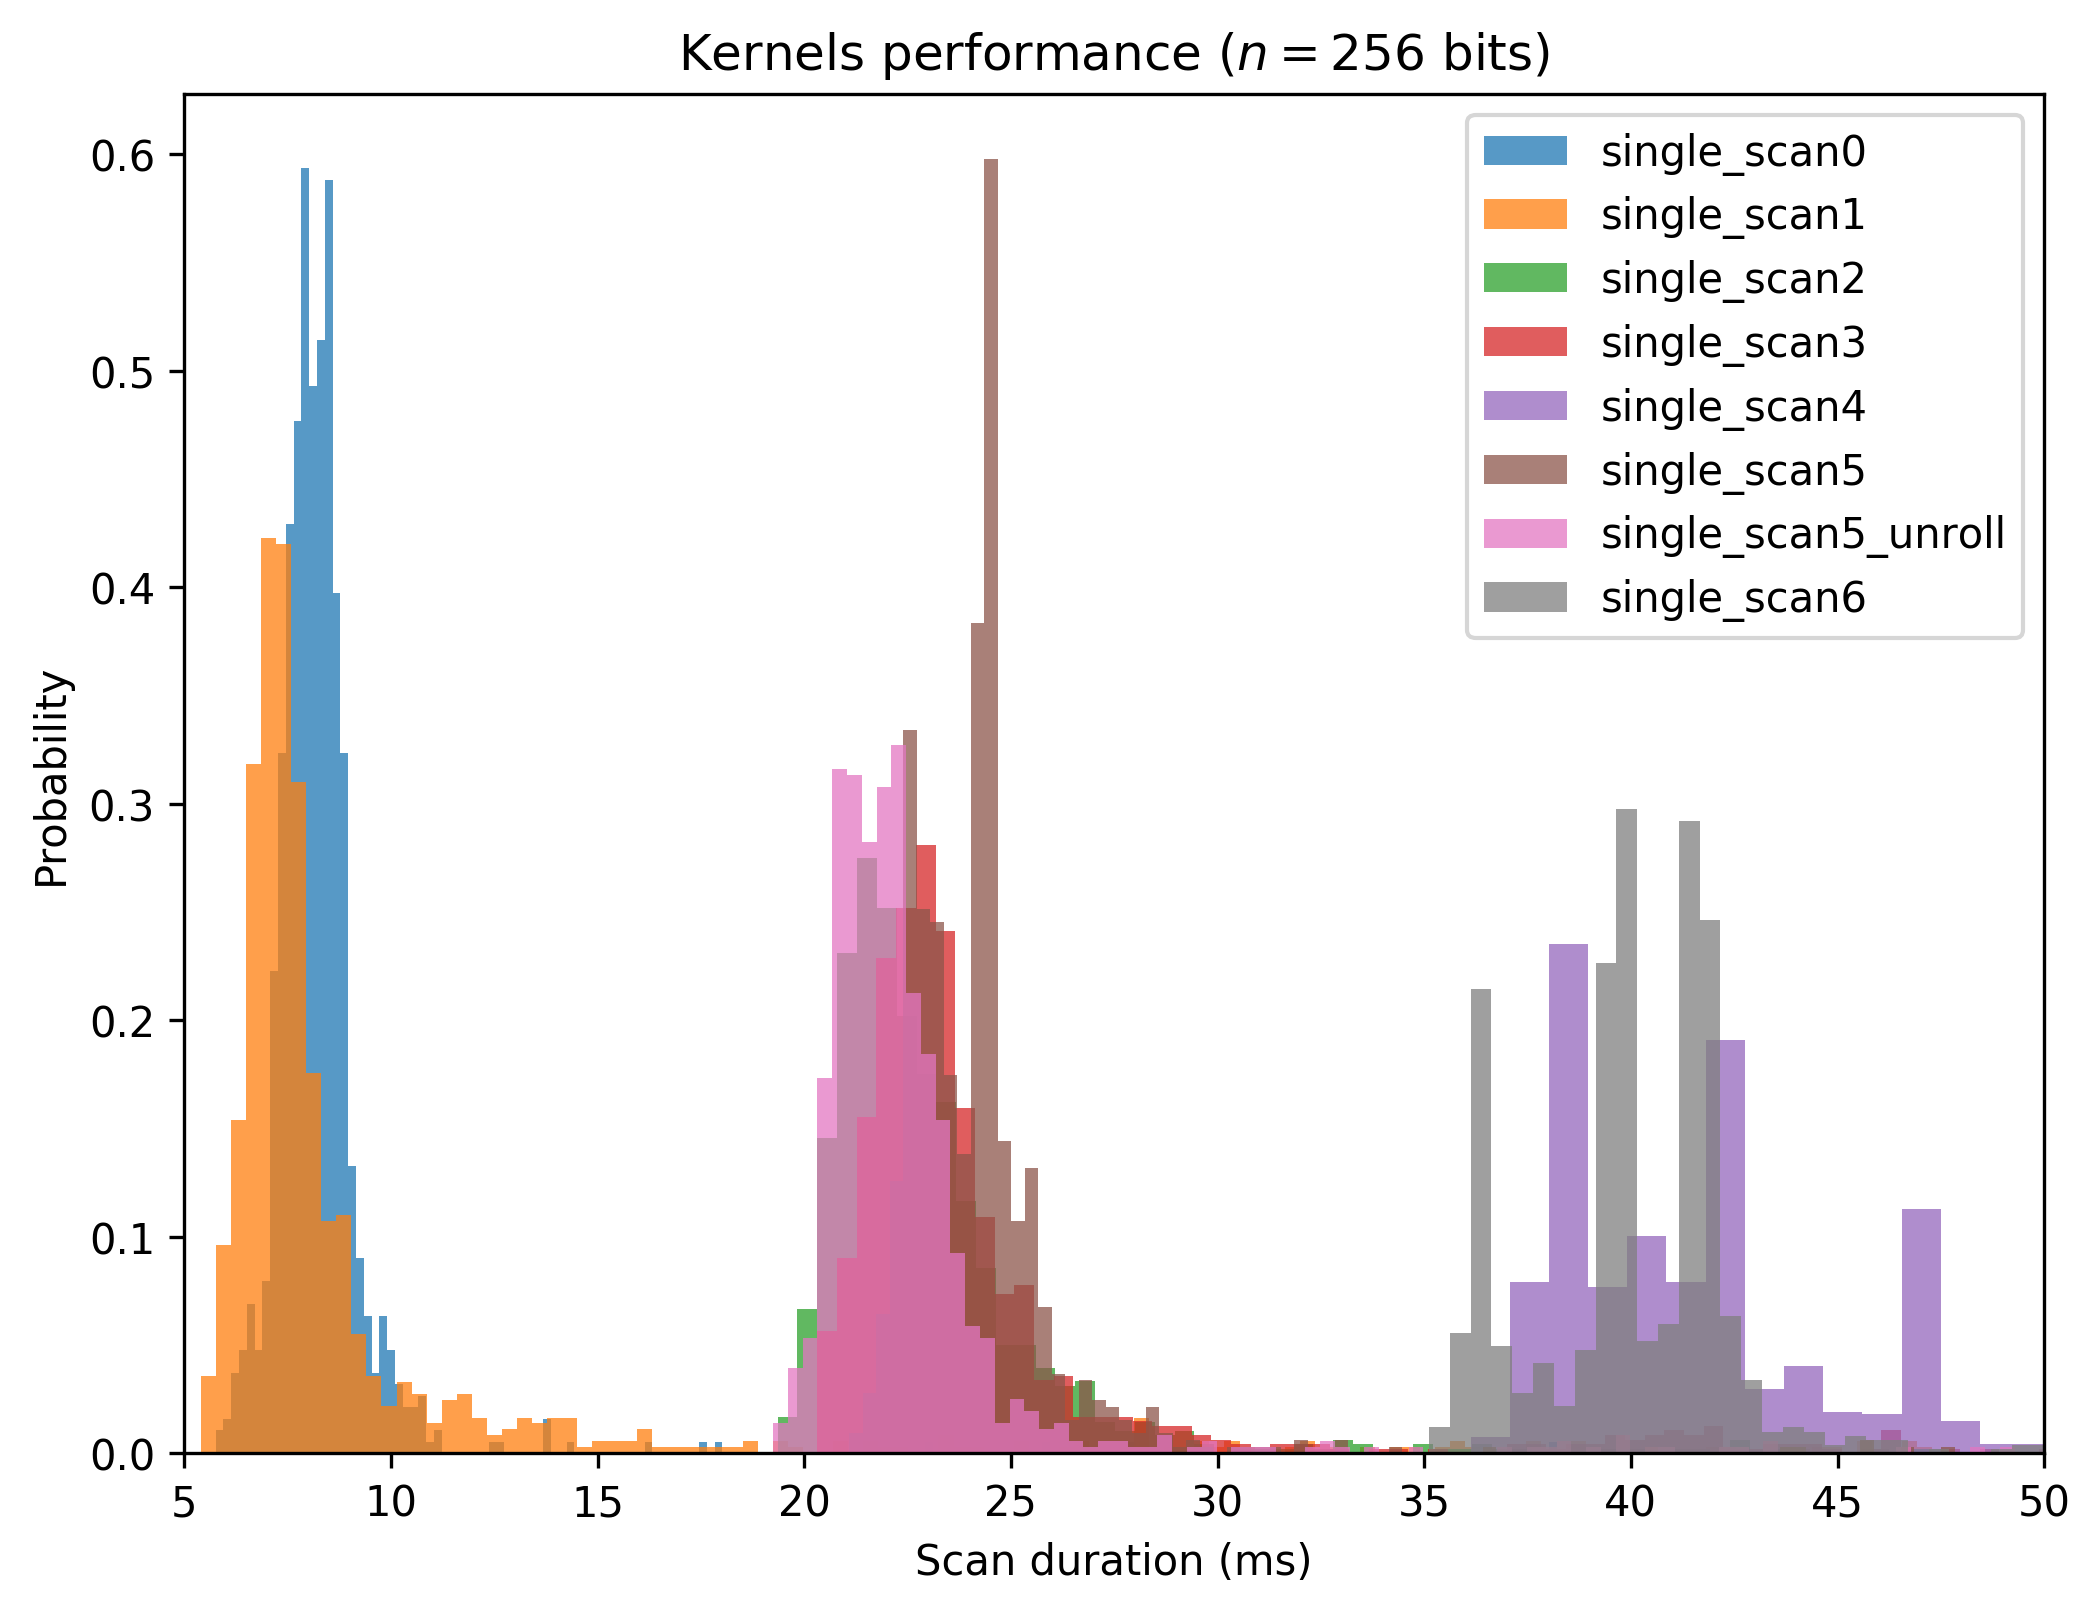
\includegraphics[width=\textwidth]{images02/performance/macbook-kernels-256.png}}

\subfloat[$n=1,000$, $r=451$, and $H=1,000,000$]{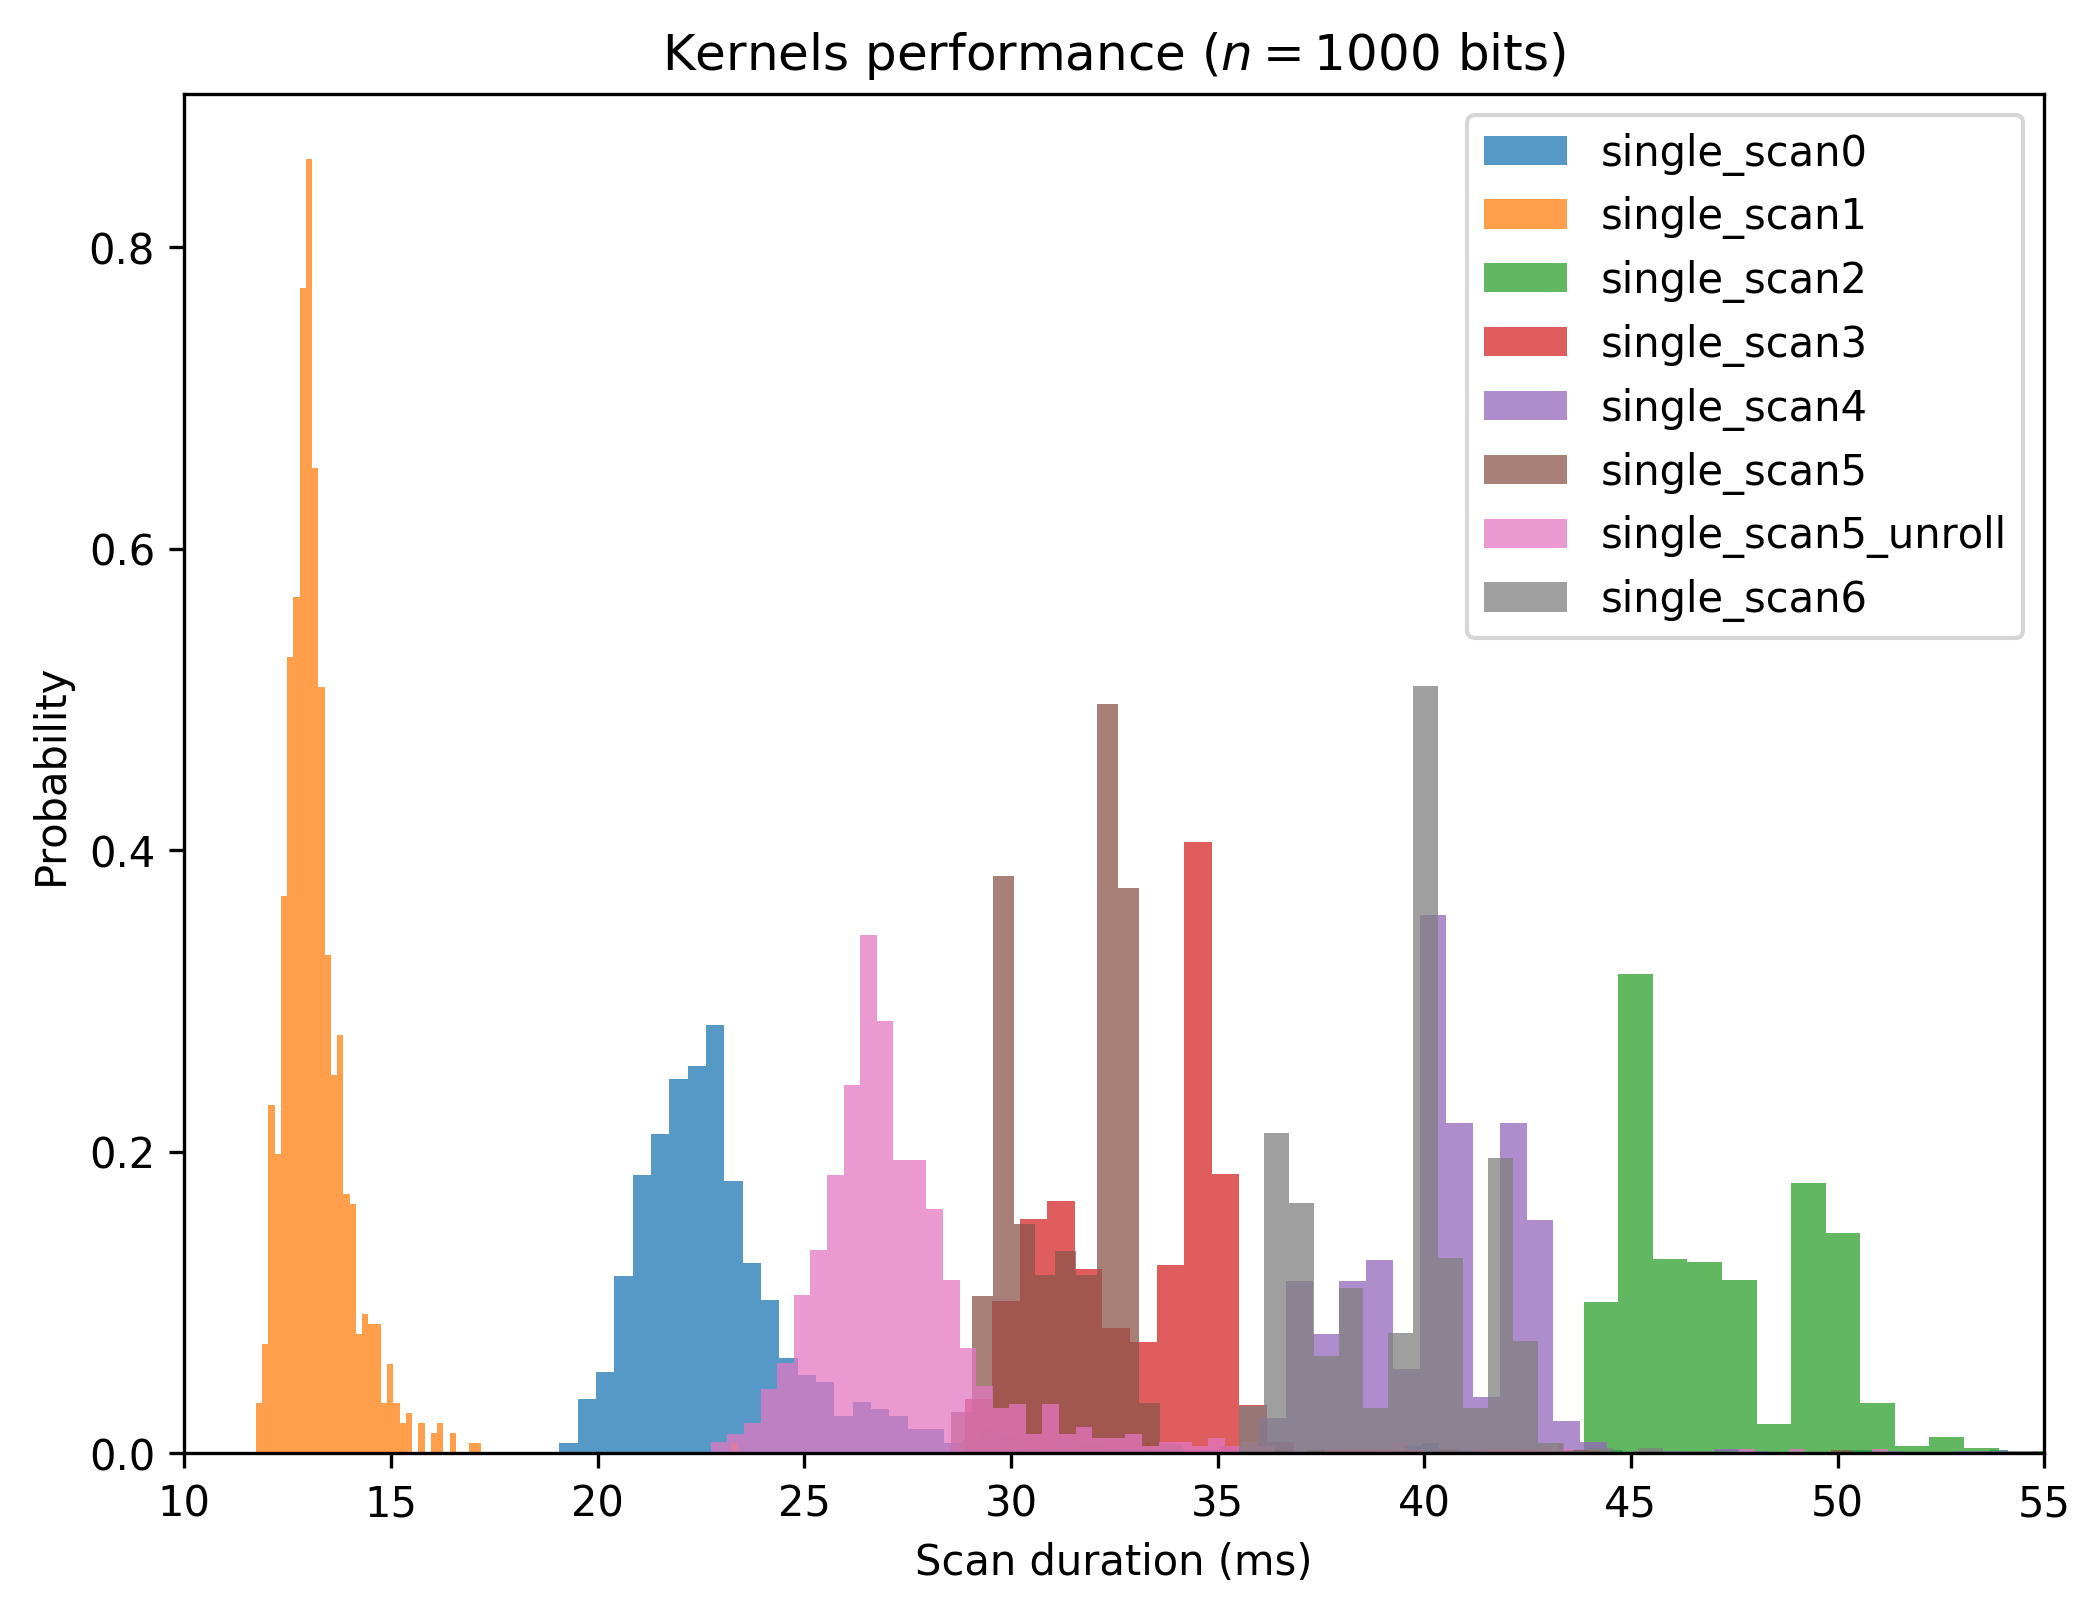
\includegraphics[width=\textwidth]{images02/performance/macbook-kernels-1000.png}}

\caption{Kernel comparisons for MacBook Pro Retina 13-inch Late 2013 with a 2.6GHz Intel core i5 processor, 6GB DDR3 RAM, and Intel Iris GPU.
\label{fig:perf-macbook-kernels}}
\end{figure}

\begin{figure}[!htb]
\centering
\subfloat[$n=1,000$, $r=451$, and $H=1,000,000$]{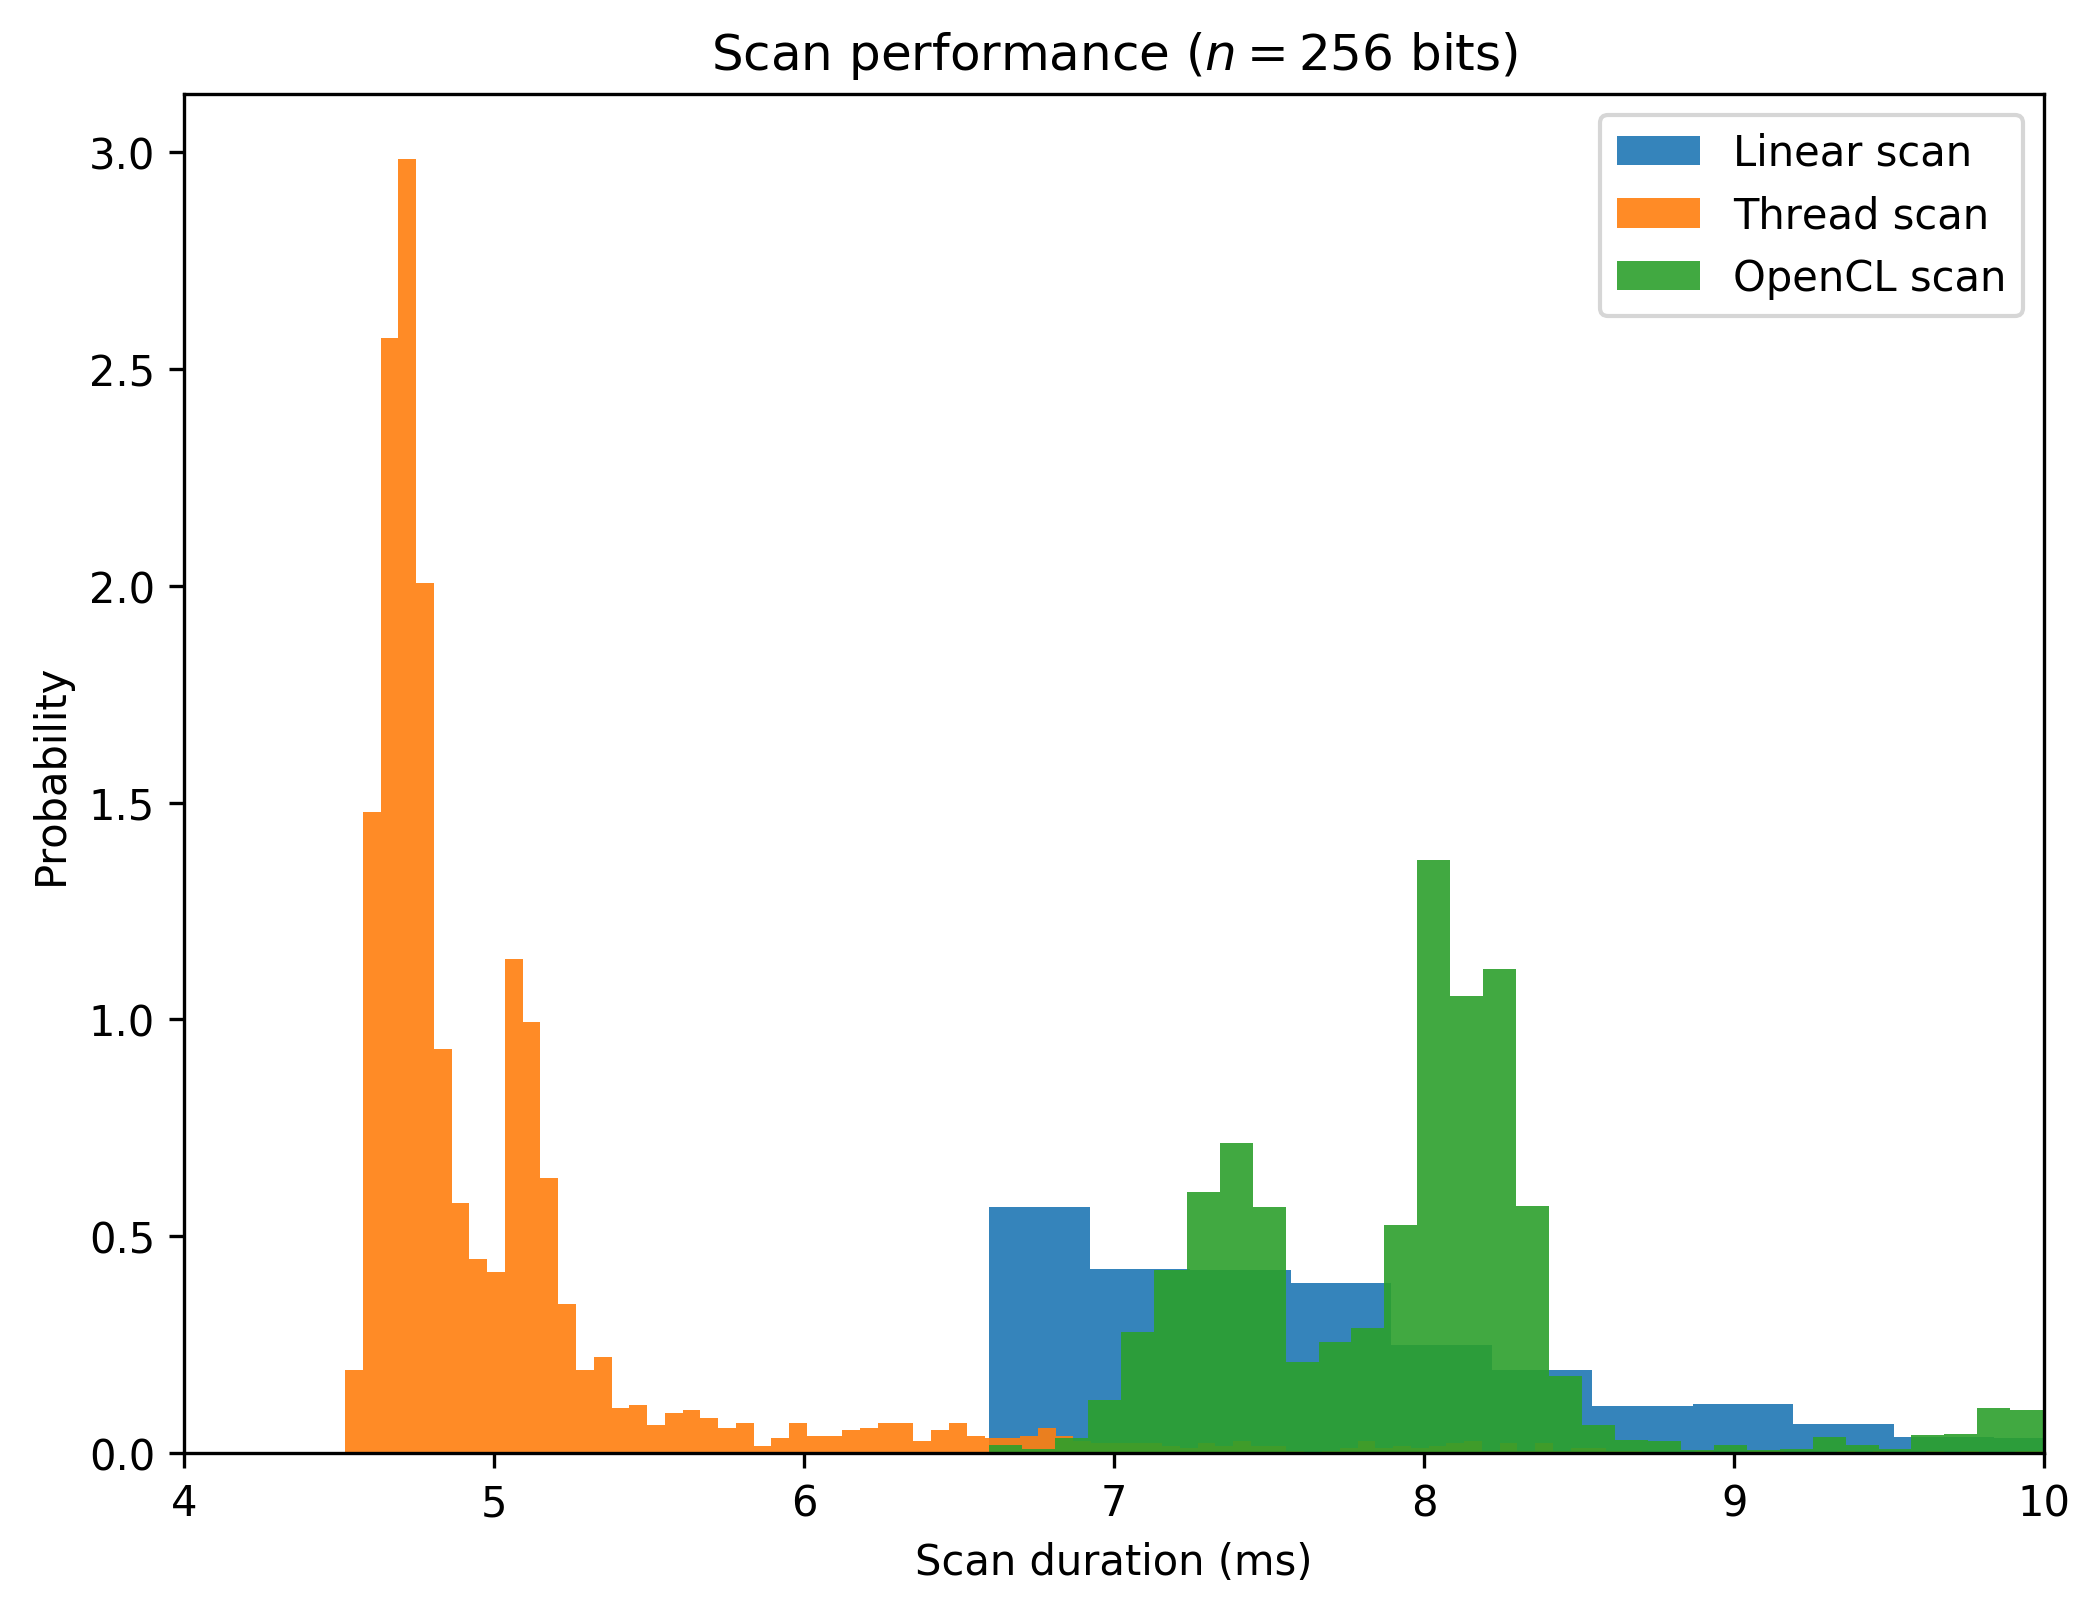
\includegraphics[width=\textwidth]{images02/performance/macbook-scan-256.png}}

\subfloat[$n=1,000$, $r=451$, and $H=1,000,000$]{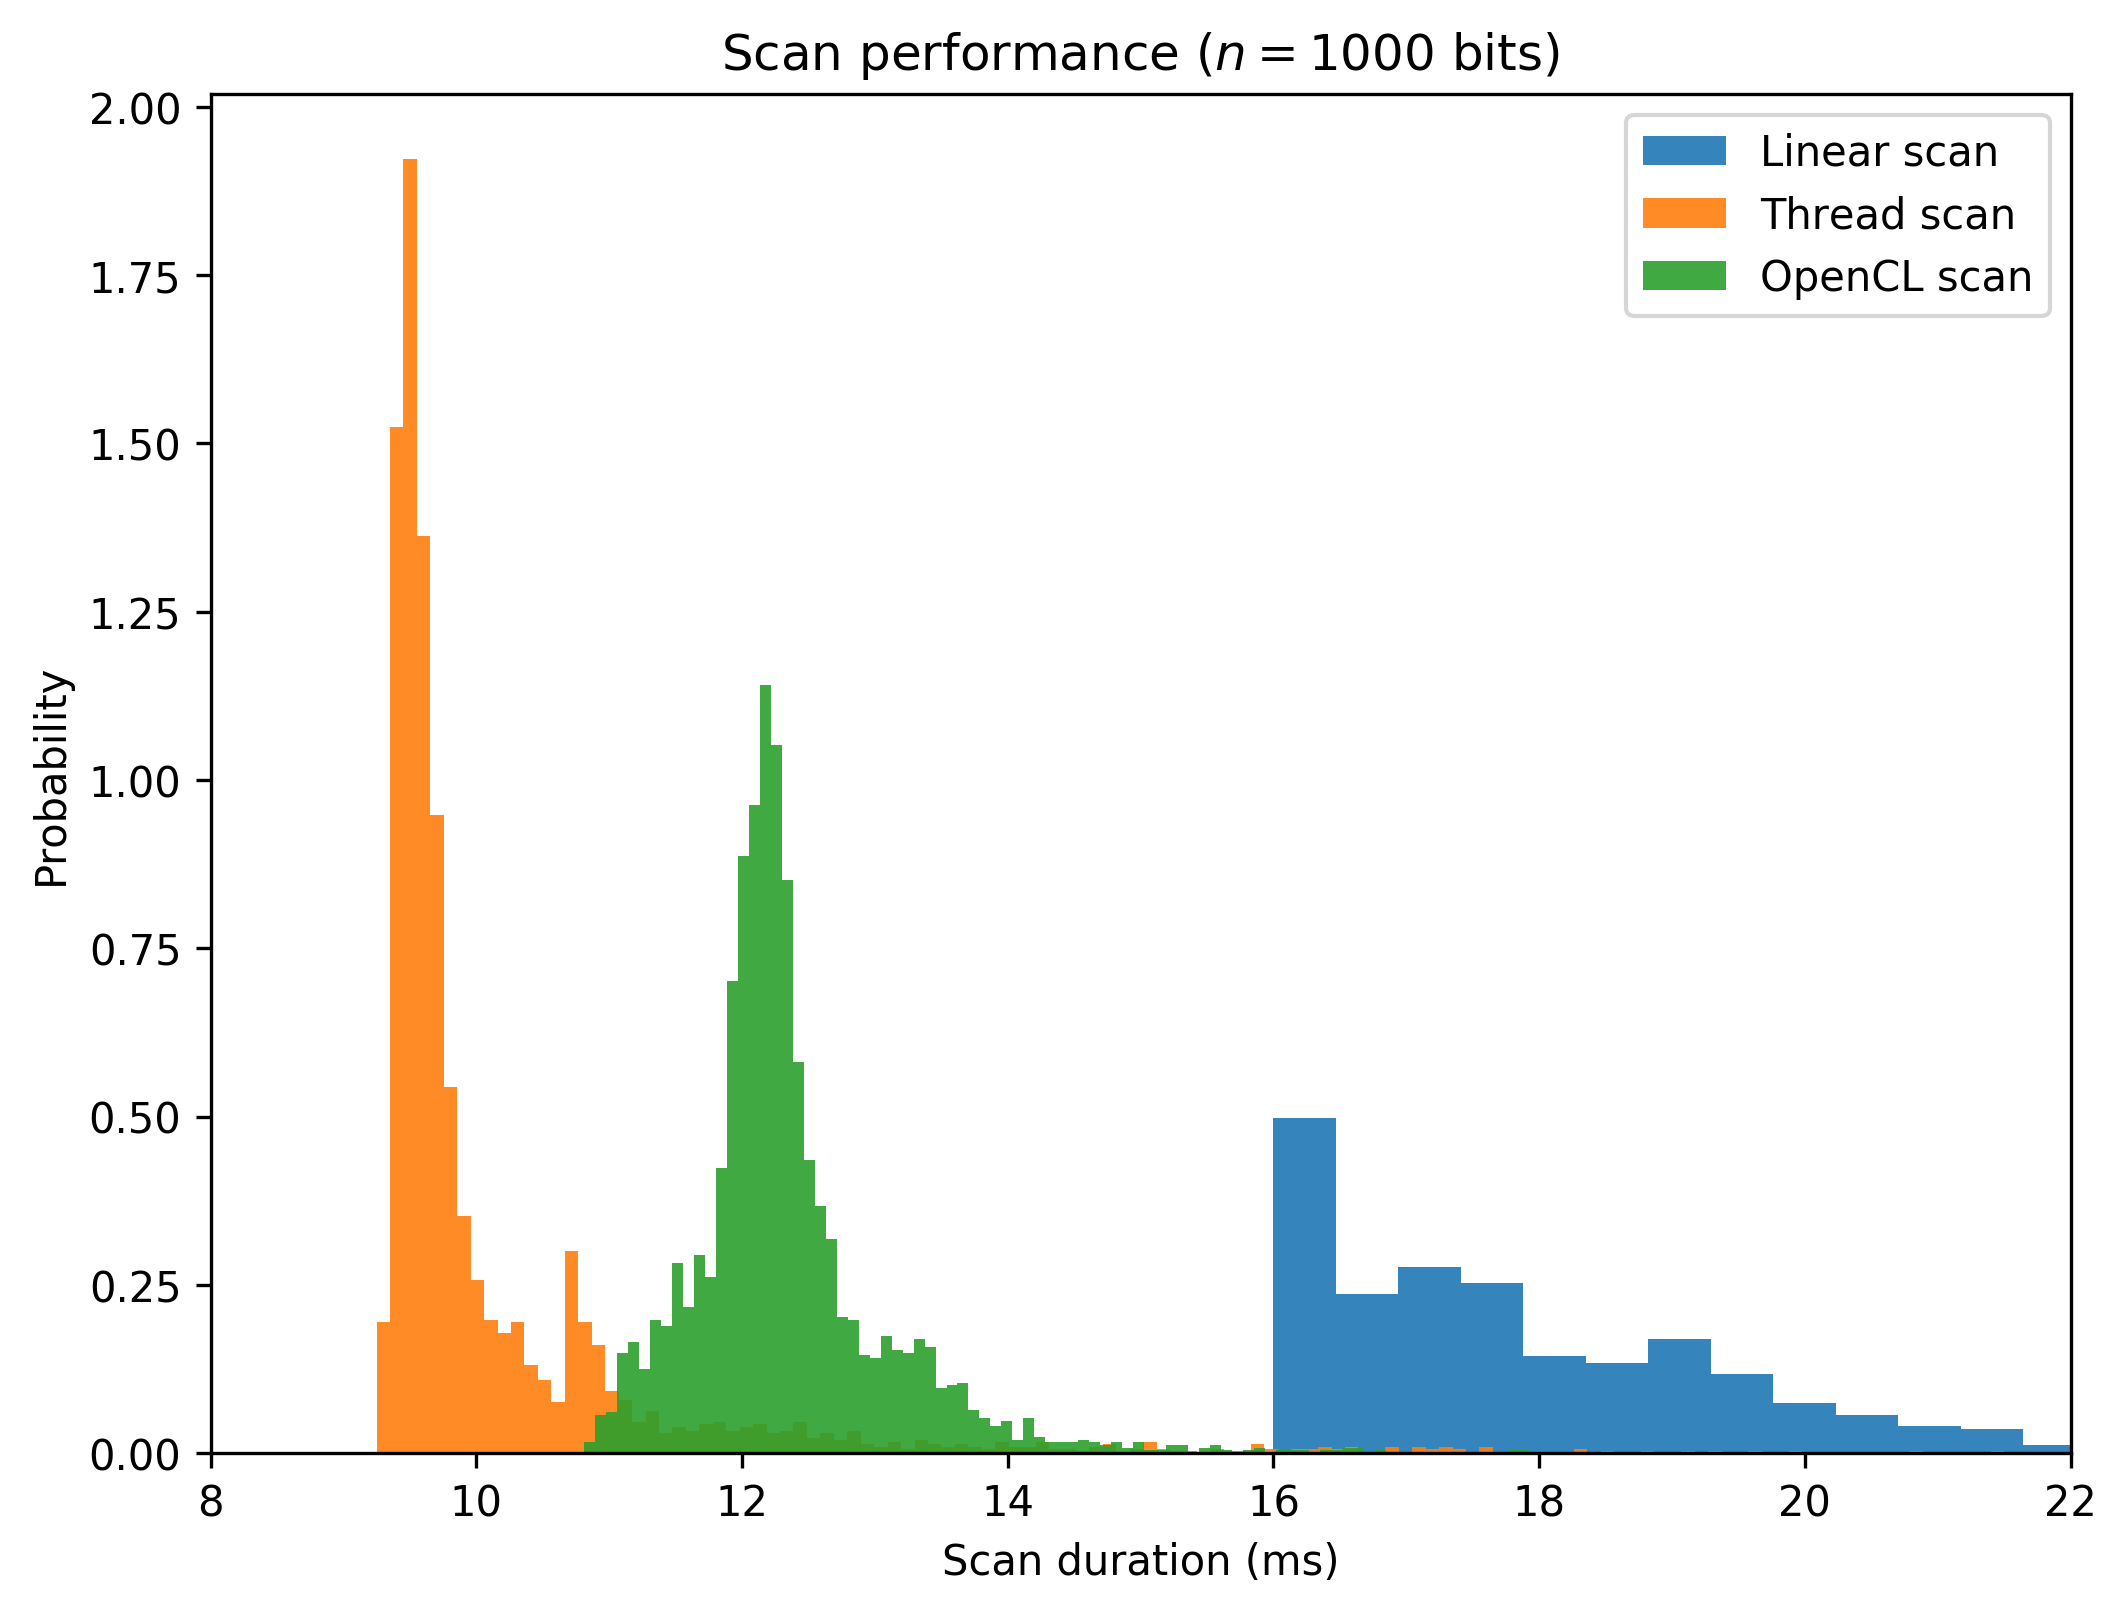
\includegraphics[width=\textwidth]{images02/performance/macbook-scan-1000.png}}

\caption{Scanner comparisons for MacBook Pro Retina 13-inch Late 2013 with a 2.6GHz Intel core i5 processor, 6GB DDR3 RAM, and Intel Iris GPU.
\label{fig:perf-macbook-scanners}}
\end{figure}


\begin{figure}[!htb]
\centering
\subfloat[$n=1,000$, $r=451$, and $H=1,000,000$]{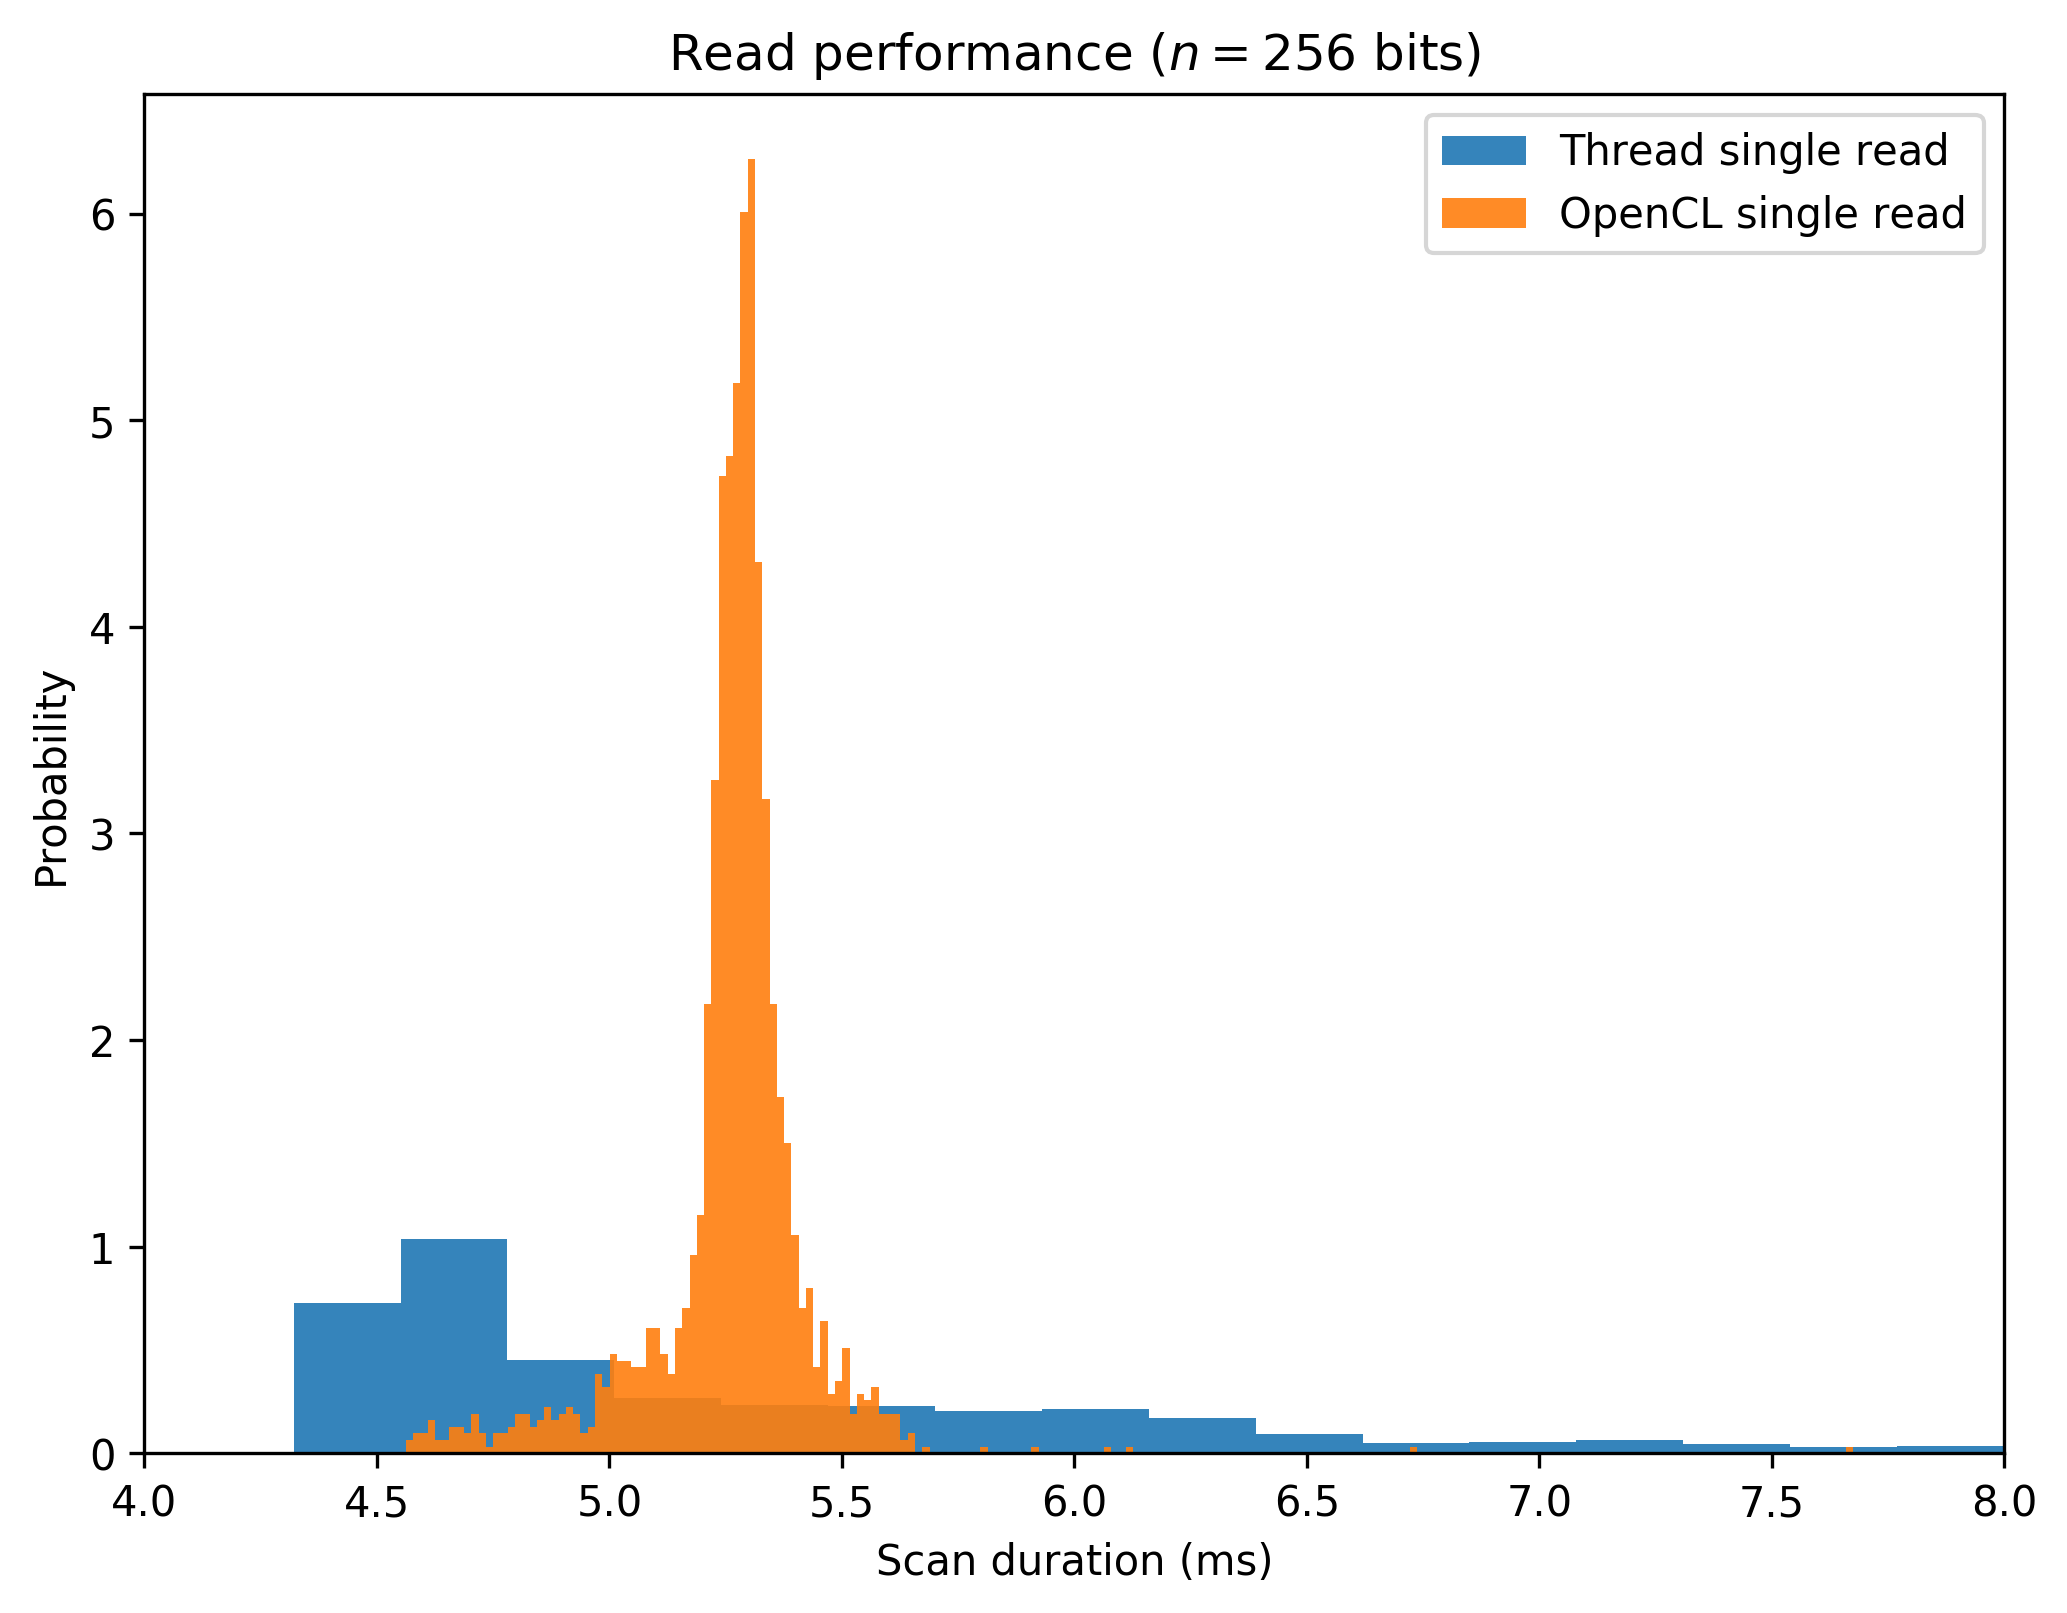
\includegraphics[width=\textwidth]{images02/performance/macbook-read-256.png}}

\subfloat[$n=1,000$, $r=451$, and $H=1,000,000$]{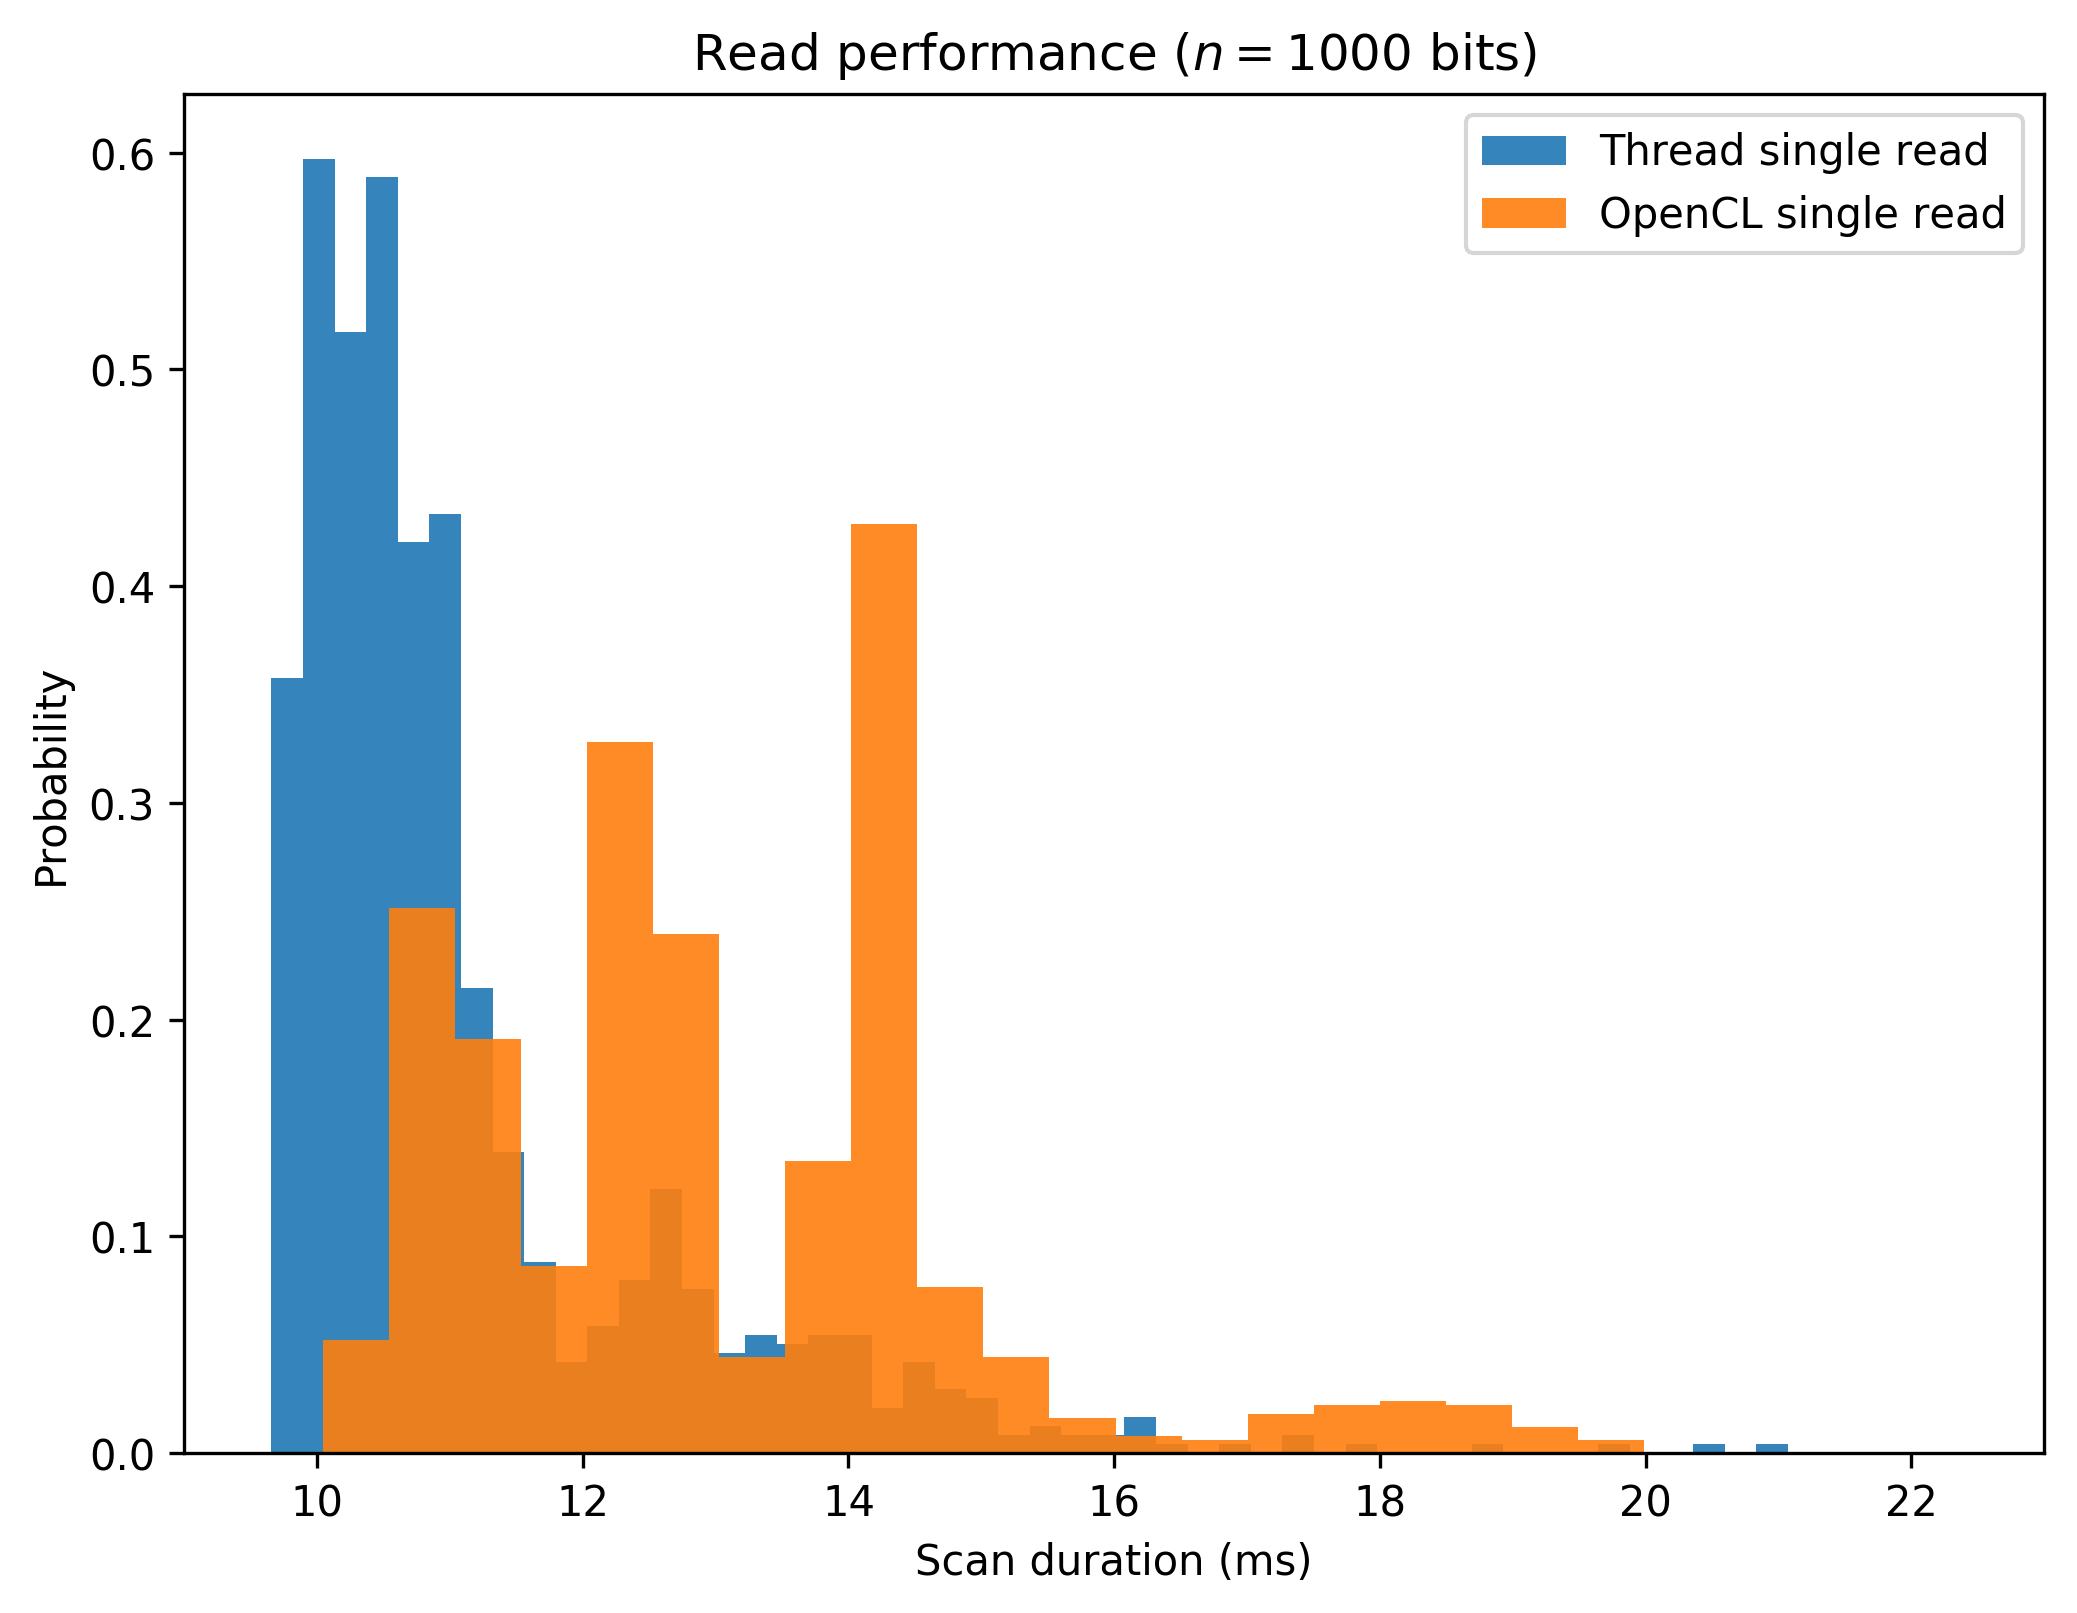
\includegraphics[width=\textwidth]{images02/performance/macbook-read-1000.png}}

\caption{Read operation comparisons for MacBook Pro Retina 13-inch Late 2013 with a 2.6GHz Intel core i5 processor, 6GB DDR3 RAM, and Intel Iris GPU.
\label{fig:perf-macbook-read}}
\end{figure}

\begin{figure}[!htb]
\centering
\subfloat[$n=1,000$, $r=451$, and $H=1,000,000$]{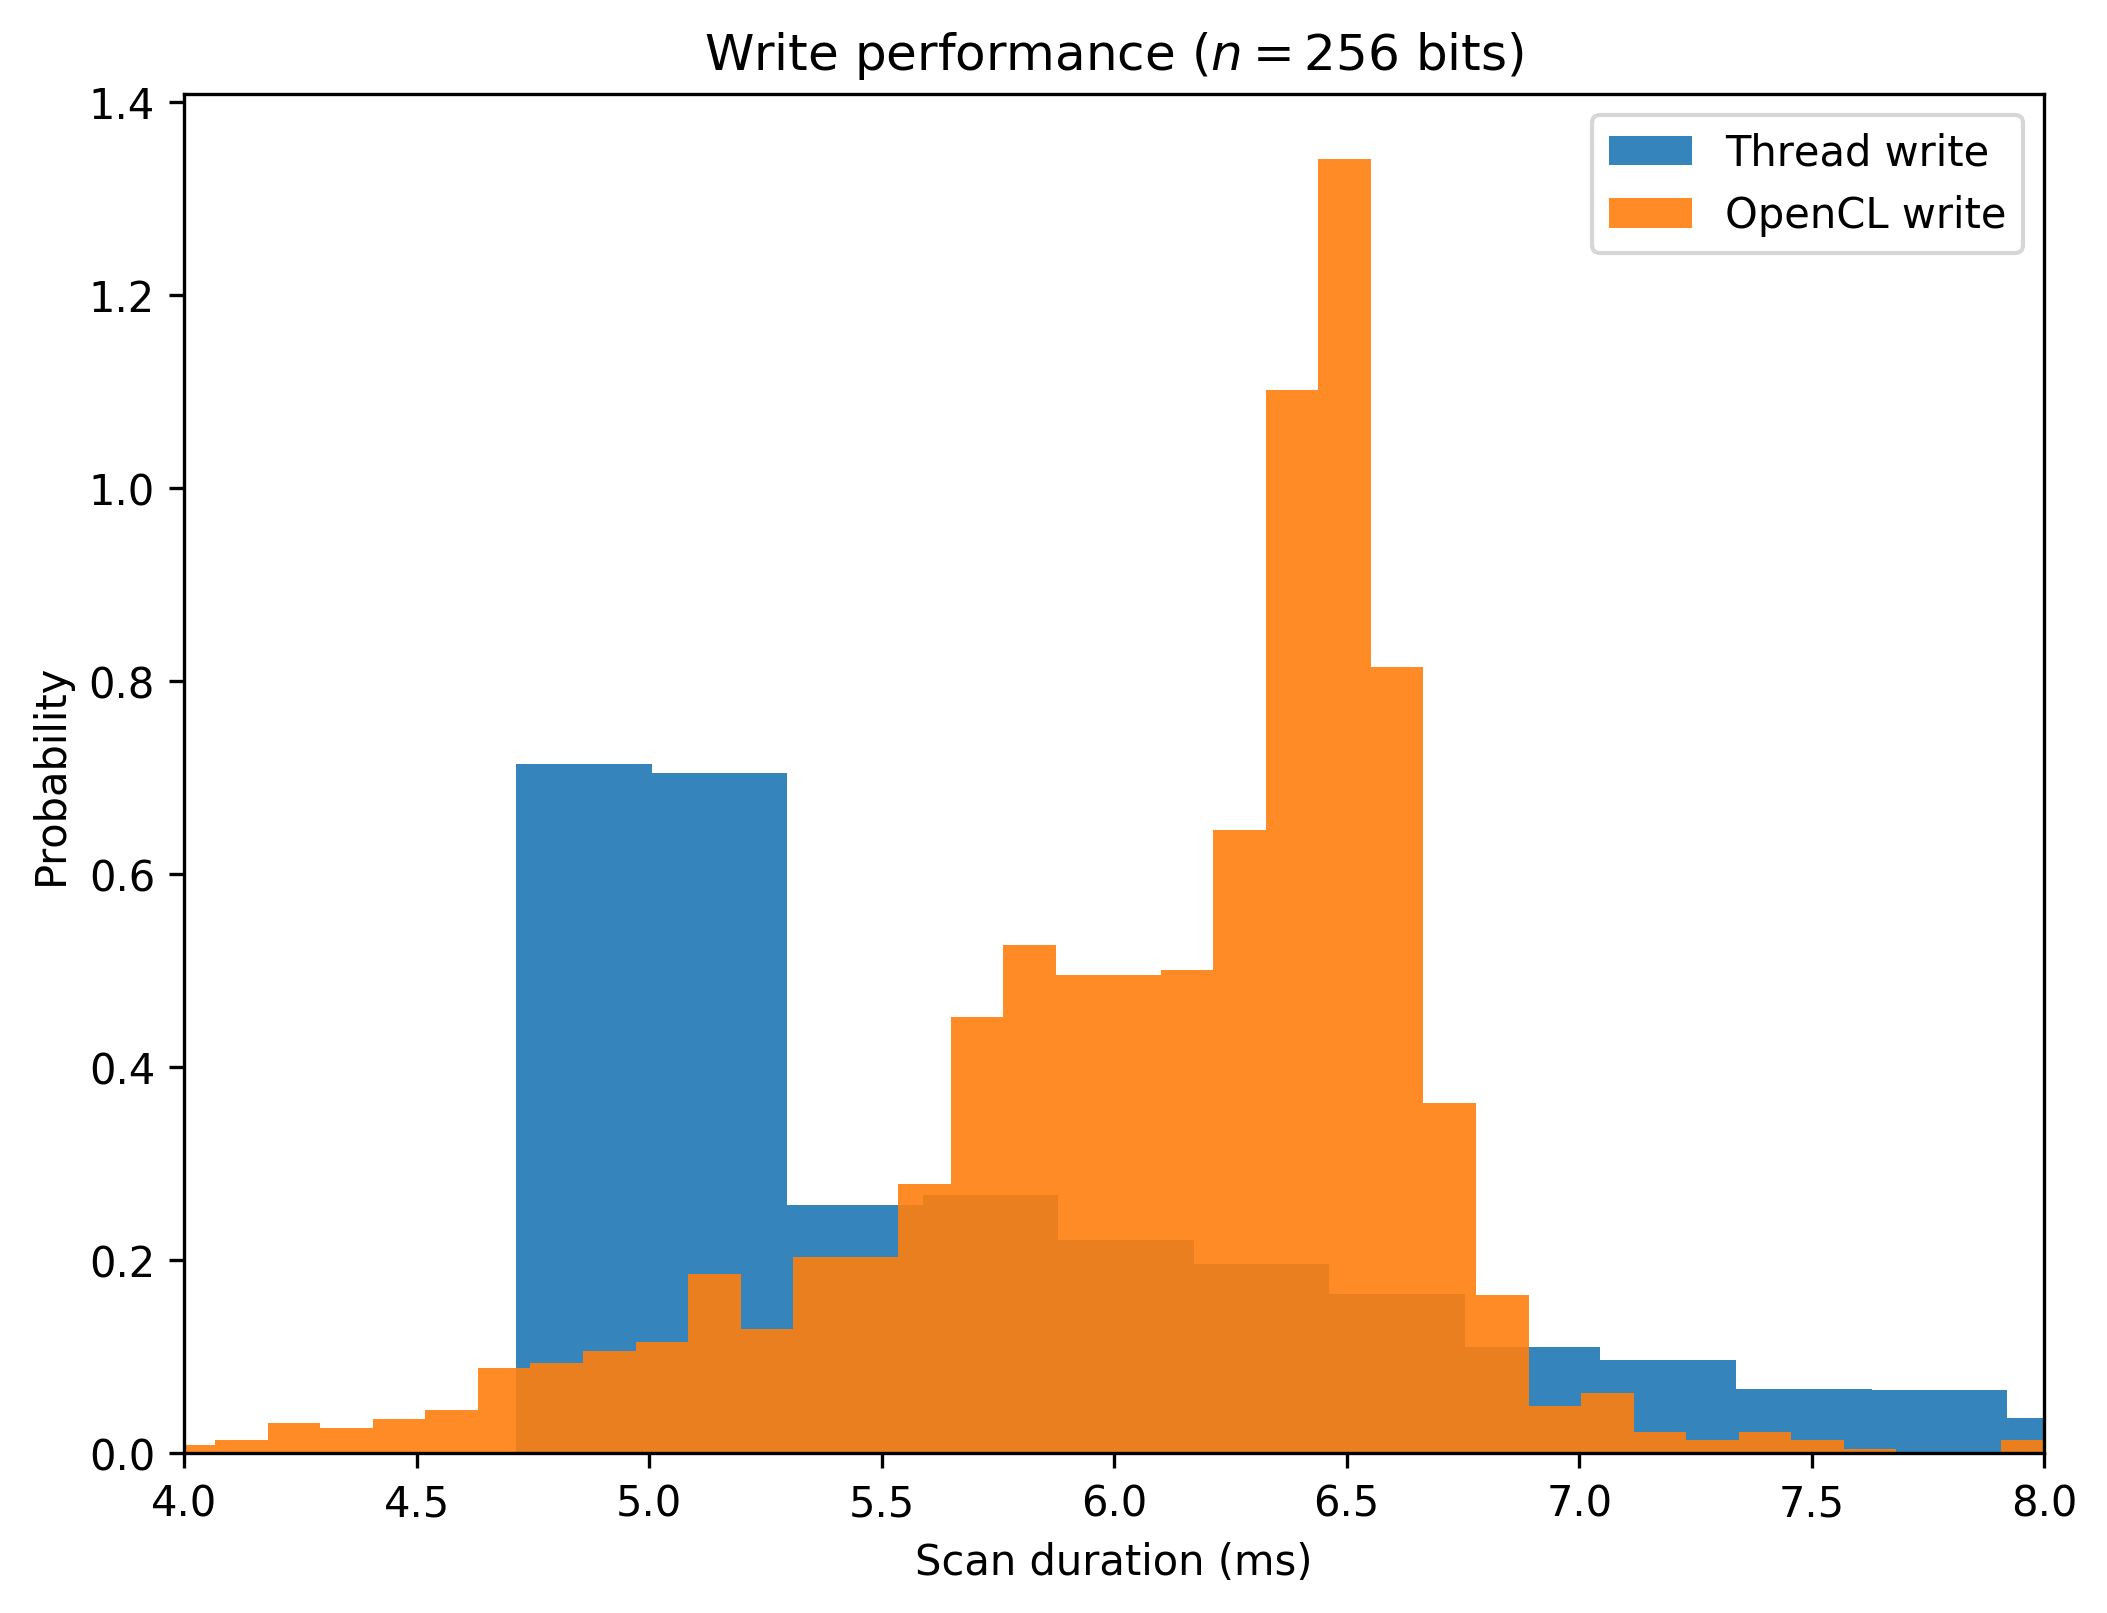
\includegraphics[width=\textwidth]{images02/performance/macbook-write-256.png}}

\subfloat[$n=1,000$, $r=451$, and $H=1,000,000$]{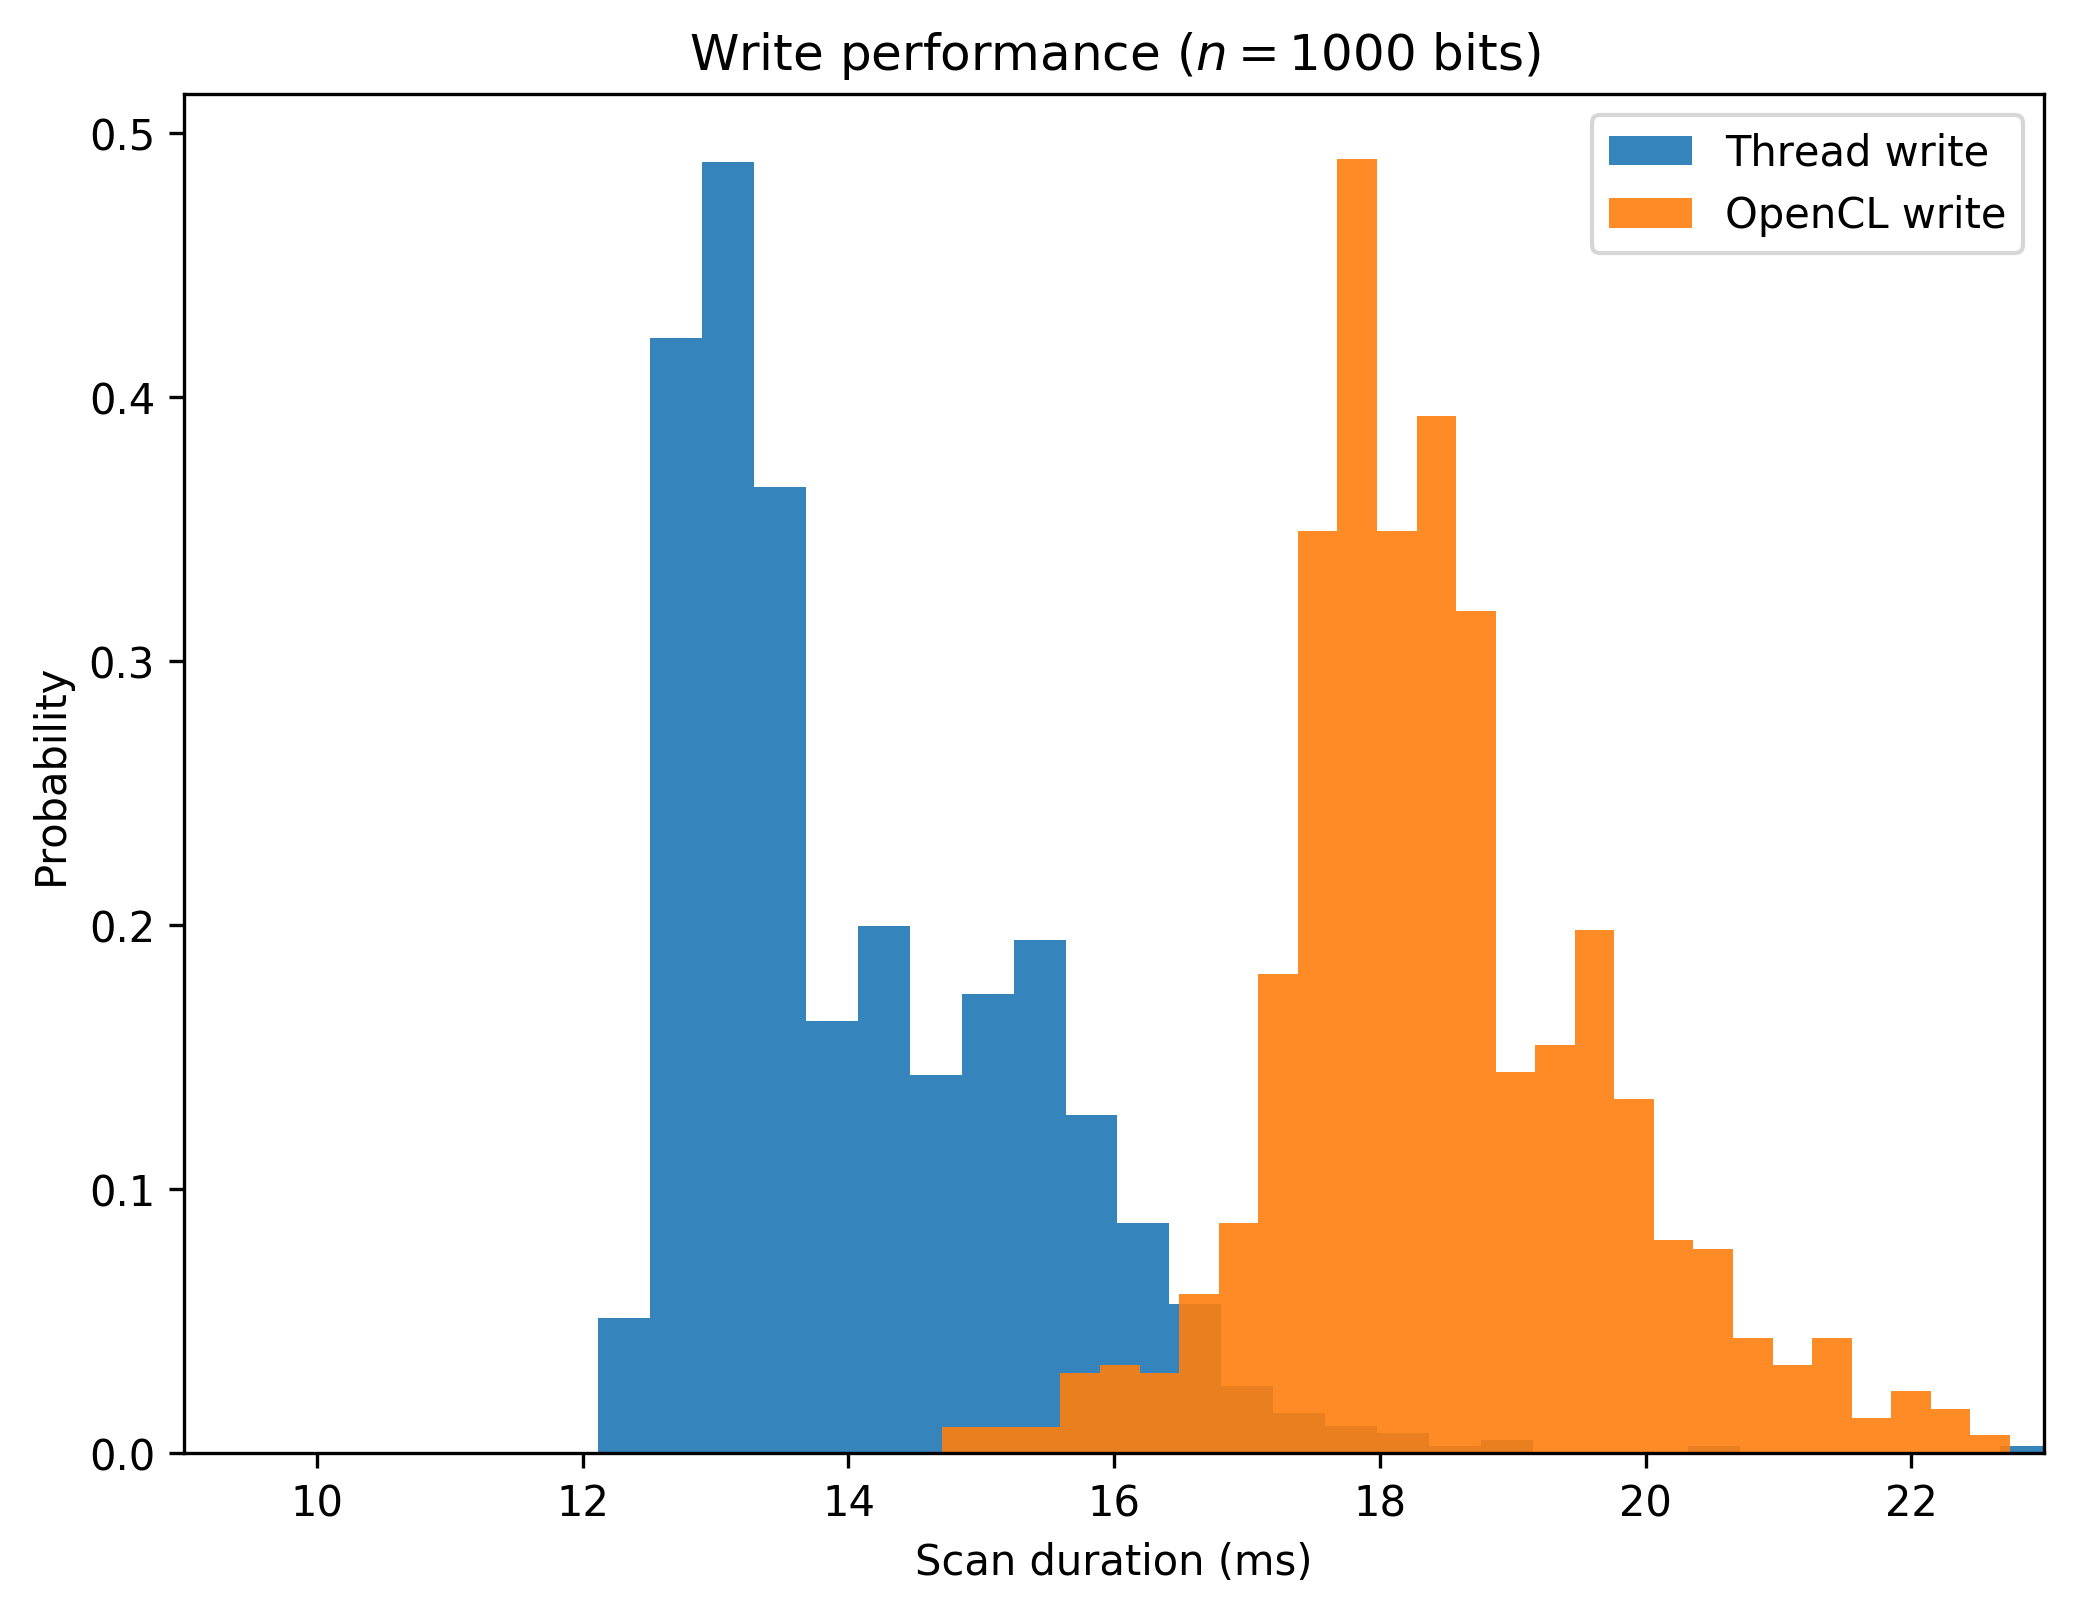
\includegraphics[width=\textwidth]{images02/performance/macbook-write-1000.png}}

\caption{Write operation comparisons for MacBook Pro Retina 13-inch Late 2013 with a 2.6GHz Intel core i5 processor, 6GB DDR3 RAM, and Intel Iris GPU.
\label{fig:perf-macbook-write}}
\end{figure}


% -------------------------
% -------------------------
% -------------------------


\begin{table}[!htb]
\centering
\begin{tabular}{lrrrr}
    \toprule
    & \textbf{256 bits} & \textbf{1,000 bits} & \textbf{10,000 bits} \\ \hline
    \hline
	Kernel & Duration (ms) & Duration (ms) & Duration (ms) \\ \hline
    single\_scan0 & 3.03 & 5.00 & 61.06 \\
    single\_scan1 & 2.87 & 3.95 & 44.96 \\
    single\_scan2 & 3.82 & 4.57 & 44.98 \\
    single\_scan3 & 3.72 & 3.68 & 12.67 \\
    single\_scan4 & 4.48 & 4.04 & 11.45 \\
    single\_scan5 & 3.76 & 3.72 & 12.58 \\
	single\_scan5\_unroll & 3.79 & 3.61 & 11.37 \\
	single\_scan6 & 4.36 & 4.02 & 10.96 \\ \hline
    \hline
	Scanner & Duration (ms) & Duration (ms) & Duration (ms) \\ \hline
    Linear scan & 5.04 & 12.25 & 116.38 \\
    Thread scan & 2.92 &  6.95 &  53.56 \\
    OpenCL scan & 2.81 &  4.20 &  12.95 \\ \hline
    \hline
	Operation & Duration (ms) & Duration (ms) & Duration (ms) \\ \hline
    Thread write       & 3.28 & 13.34 \\
    Thread single read & 2.55 & 10.39 \\
    OpenCL write       & 2.64 &  7.90 \\
    OpenCL single read & 2.14 &  5.25 \\
    \bottomrule
\end{tabular}
\caption{iMac Retina 5K 27-inch 2017 with a 3.8GHz Intel core i5 processor, 8GB DDR4 RAM, and a Radeon Pro 580 8G GPU. The SDM settings were: (i) $n=256$, $r=103$, and $H=1,000,000$; (ii) $n=1,000$, $r=451$, and $H=1,000,000$; and (iii) $n=10,000$, $r=4850$, and $H=1,000,000$. There is no benchmark for read and write operations with $n=10,000$ because RAM is not enough to allocate the counters---it would consume 37.25 GB of RAM.
For the histogram of durations, see Figures \ref{fig:perf-imac-kernels}, \ref{fig:perf-imac-scanners}, \ref{fig:perf-imac-read}, and \ref{fig:perf-imac-write}.
\label{tab:perf-imac}}
\end{table}


\begin{figure}[!htb]
\centering
\subfloat[$n=256$, $r=103$, and $H=1,000,000$]{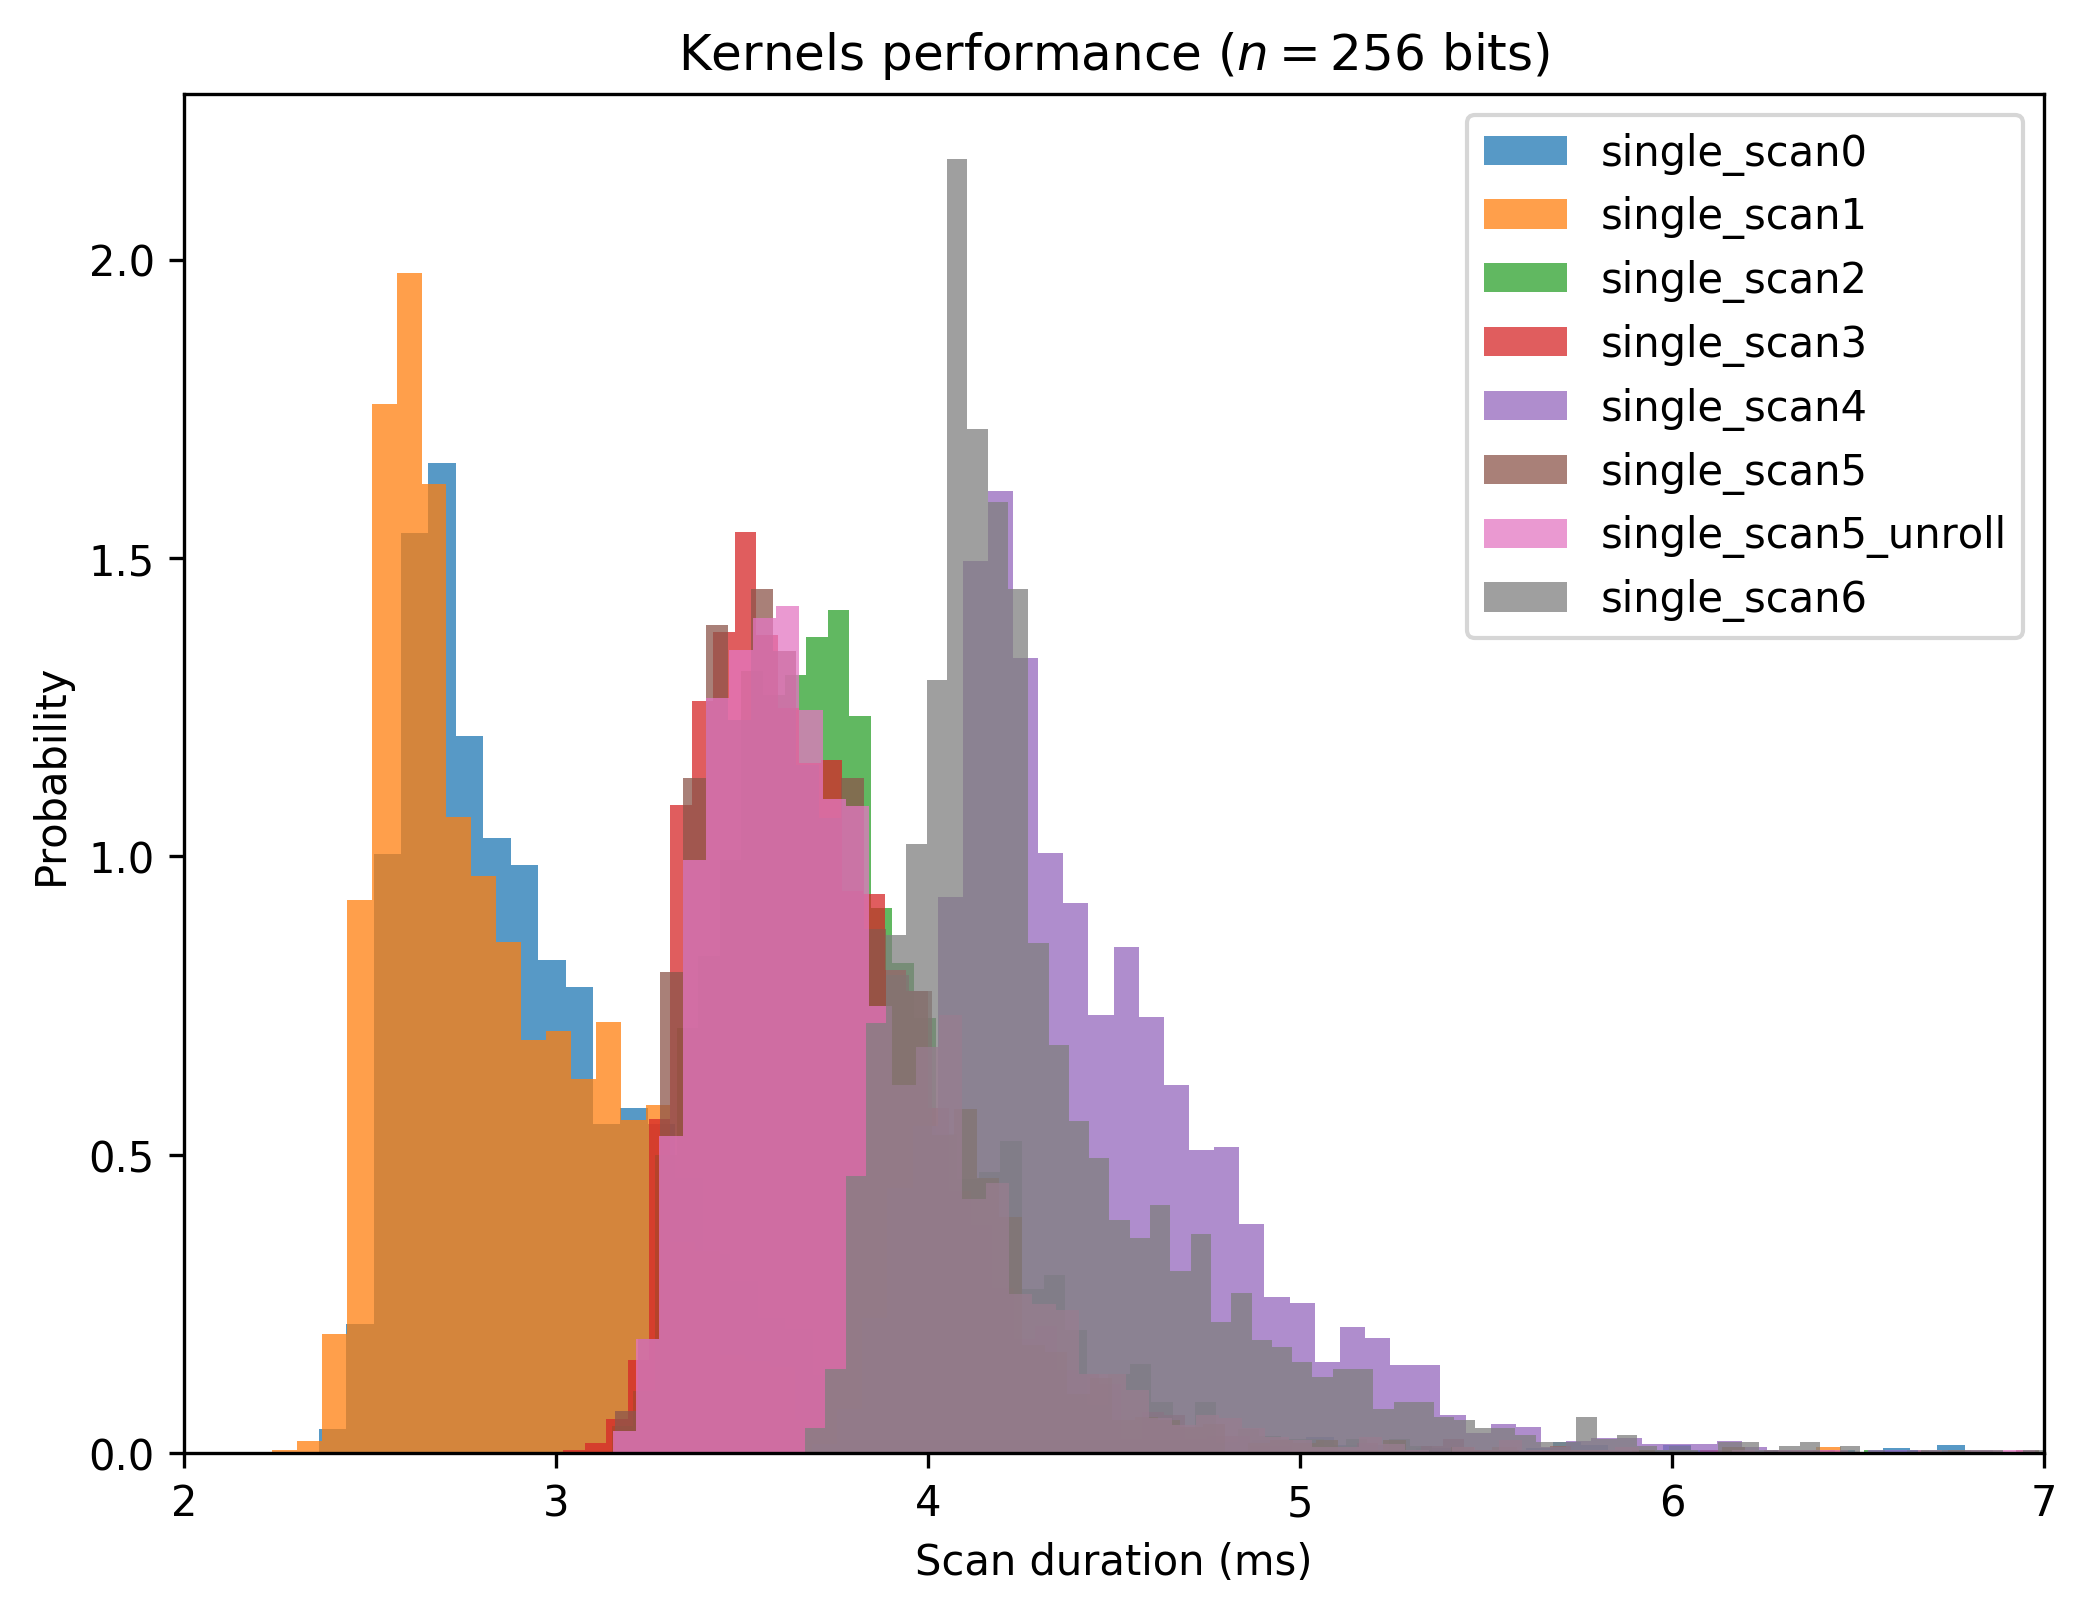
\includegraphics[width=0.7\textwidth]{images02/performance/imac-kernels-256.png}}

\subfloat[$n=1,000$, $r=451$, and $H=1,000,000$]{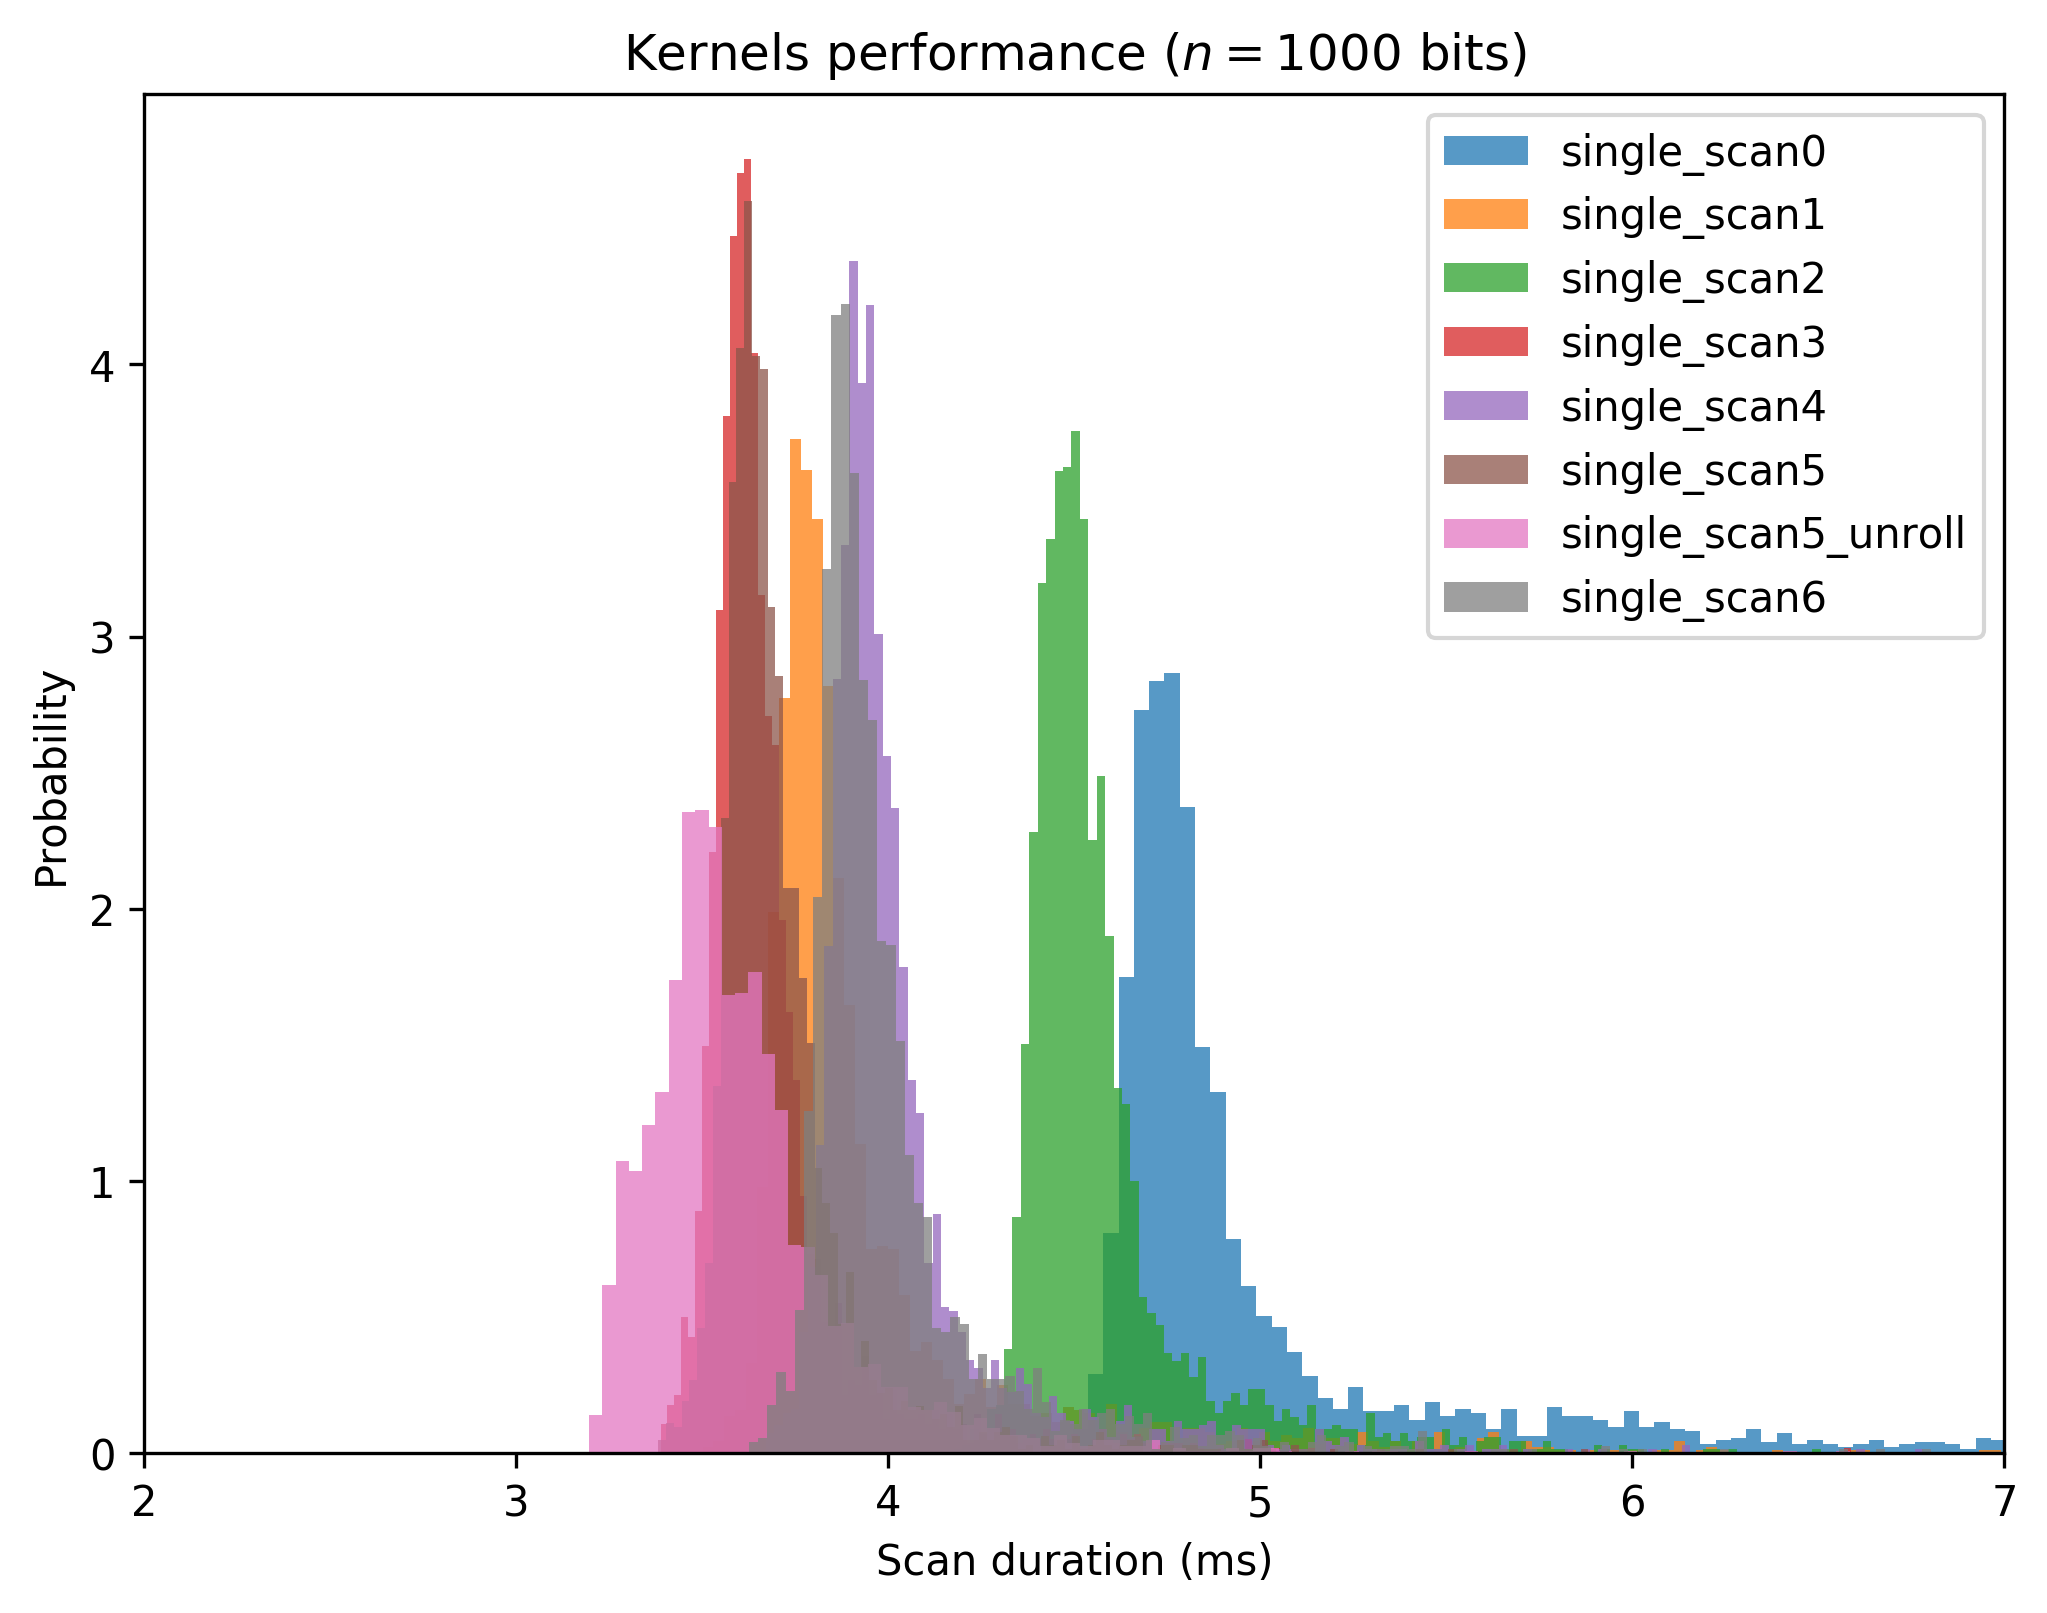
\includegraphics[width=0.7\textwidth]{images02/performance/imac-kernels-1000.png}}

\subfloat[$n=10,000$, $r=4805$, and $H=1,000,000$]{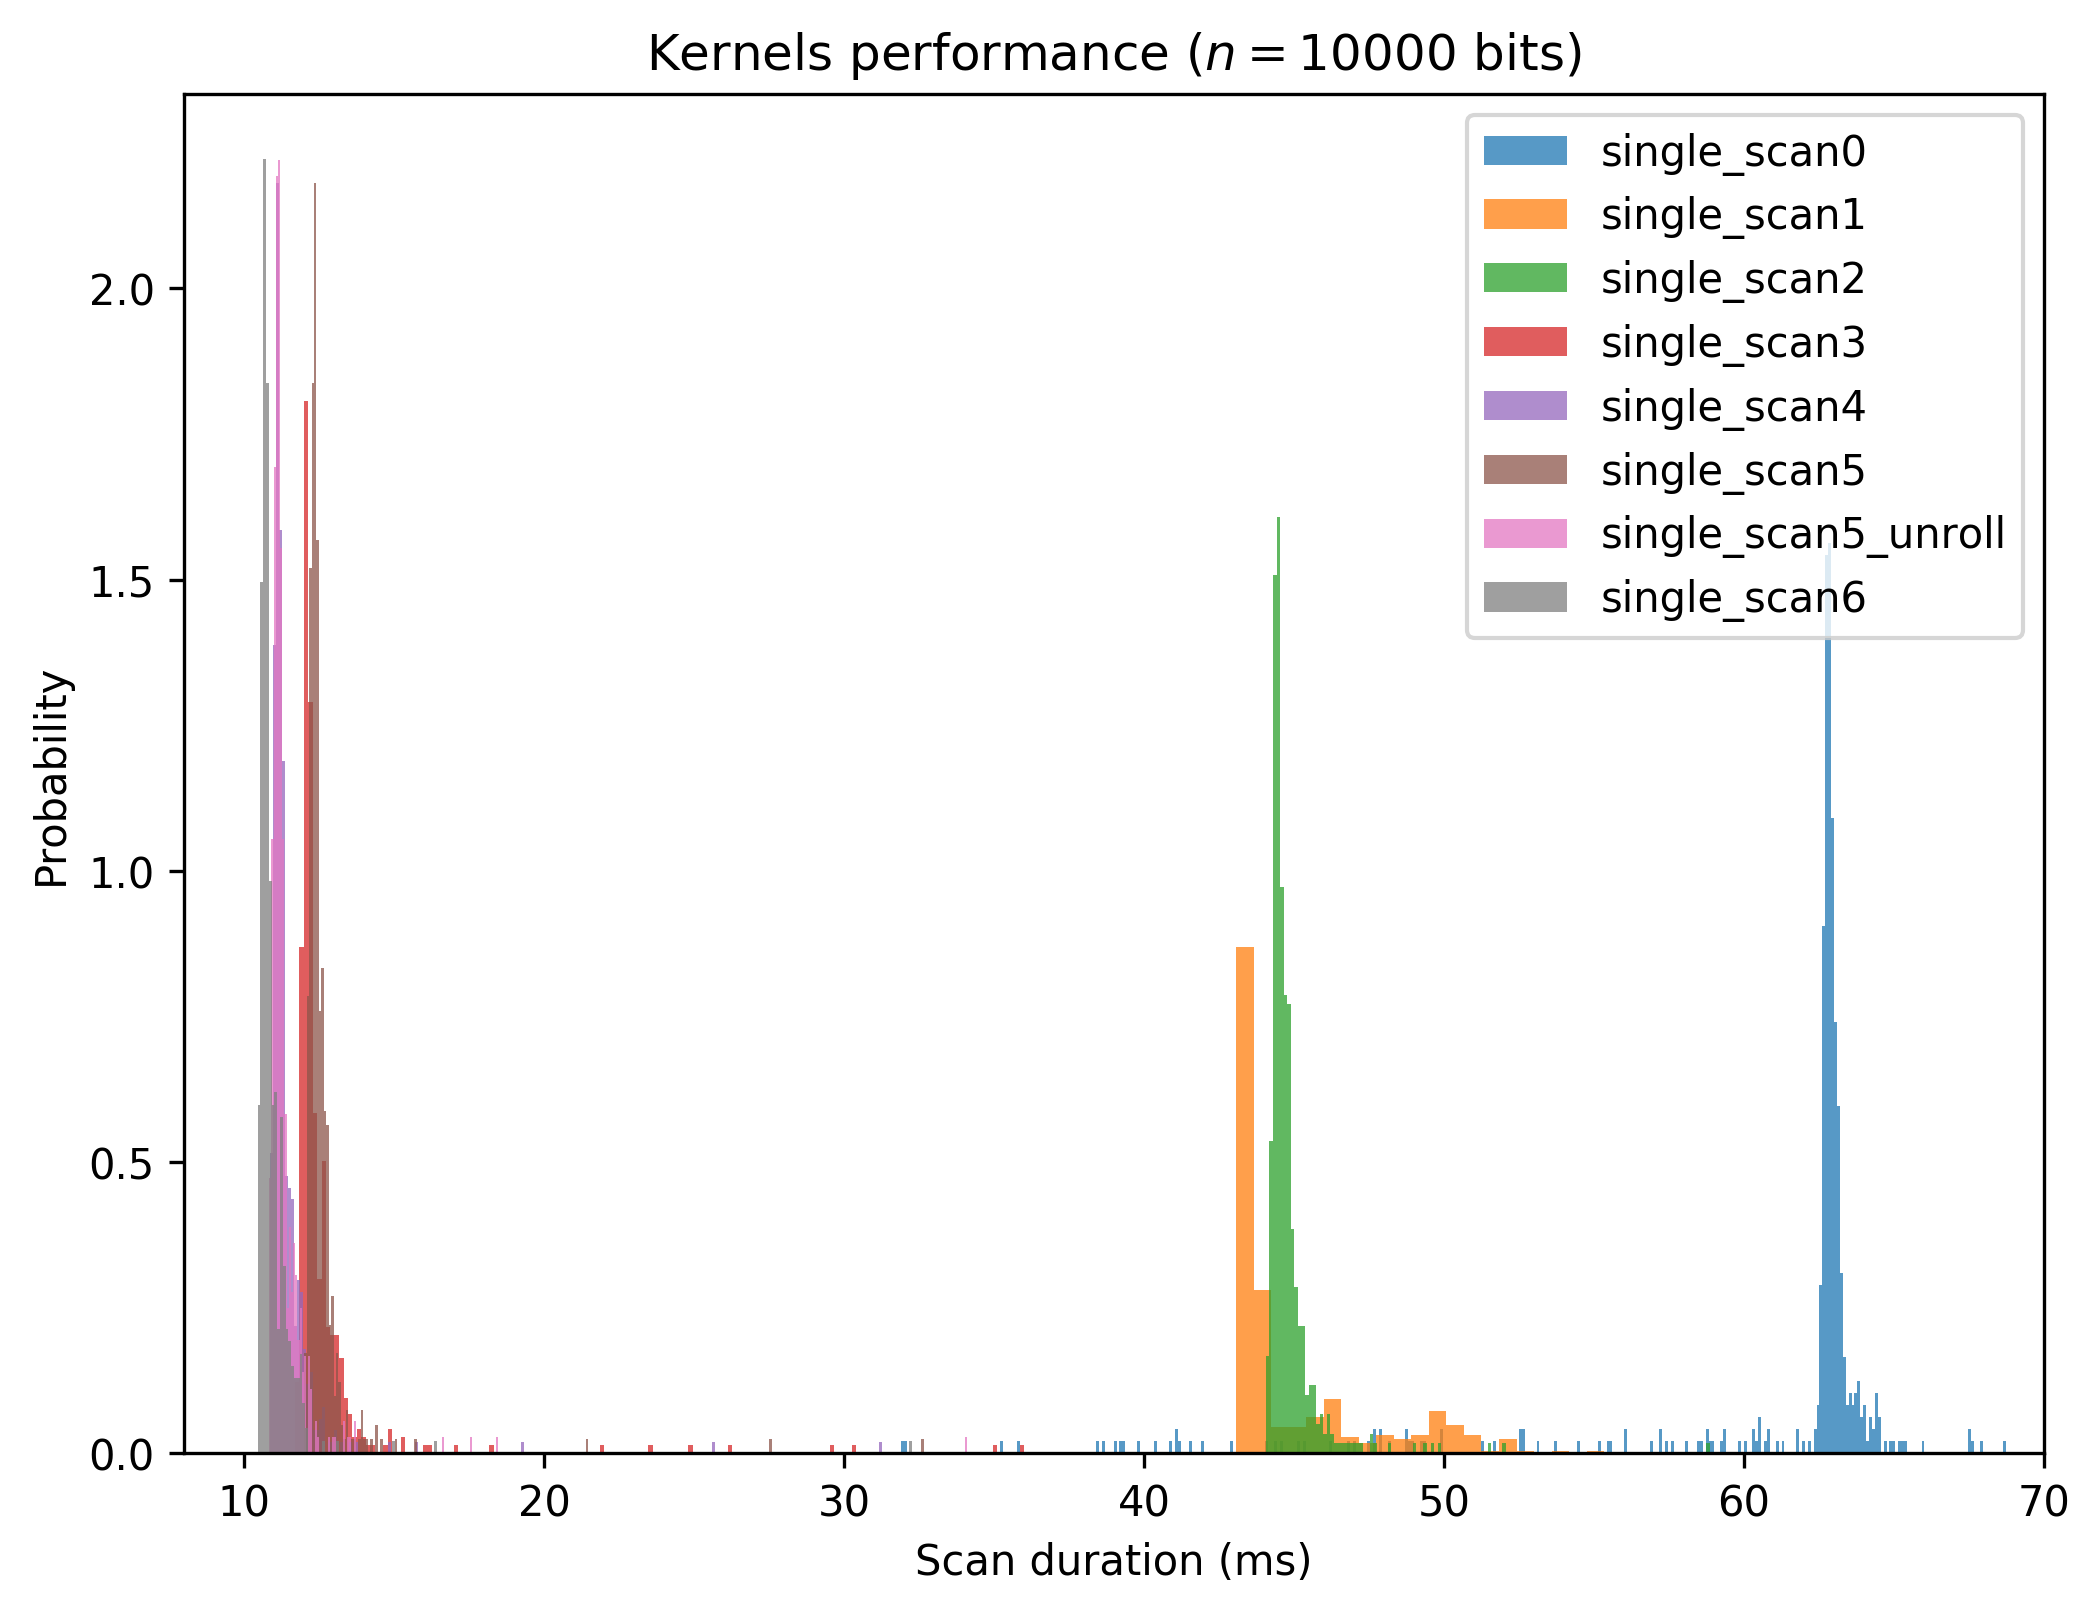
\includegraphics[width=0.7\textwidth]{images02/performance/imac-kernels-10k.png}}

\caption{Kernel comparisons for iMac Retina 5K 27-inch 2017 with a 3.8GHz Intel core i5 processor, 8GB DDR4 RAM, and a Radeon Pro 580 8G GPU.
\label{fig:perf-imac-kernels}}
\end{figure}

\begin{figure}[!htb]
\centering
\subfloat[$n=1,000$, $r=451$, and $H=1,000,000$]{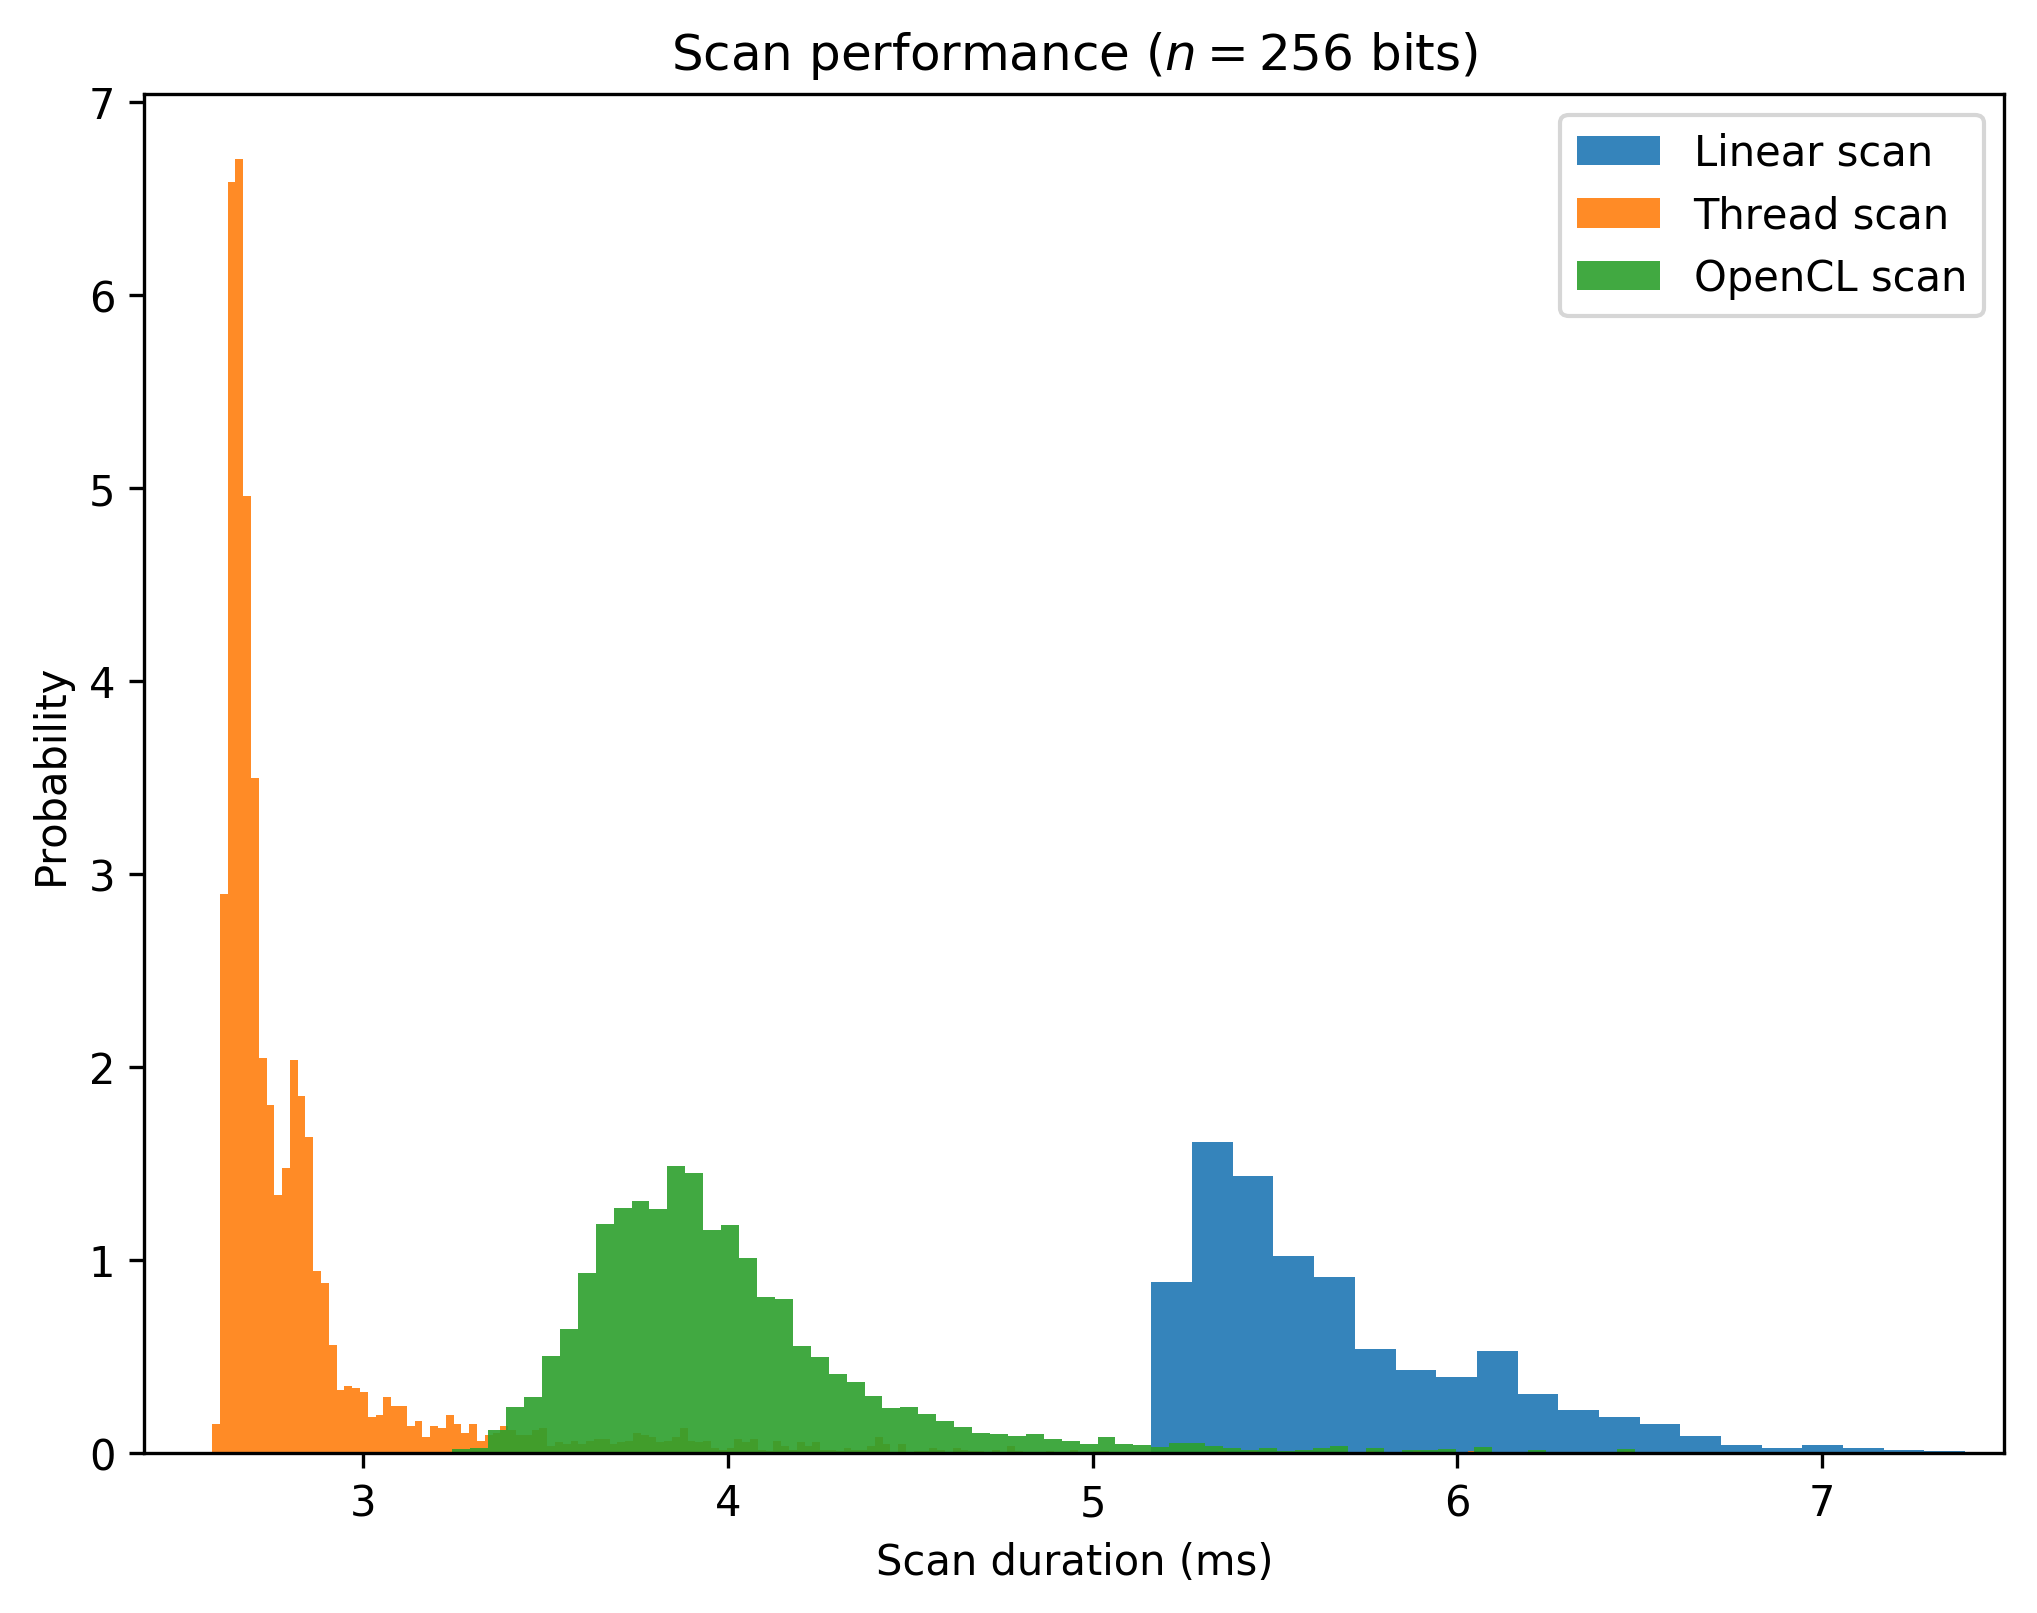
\includegraphics[width=0.7\textwidth]{images02/performance/imac-scan-256.png}}

\subfloat[$n=1,000$, $r=451$, and $H=1,000,000$]{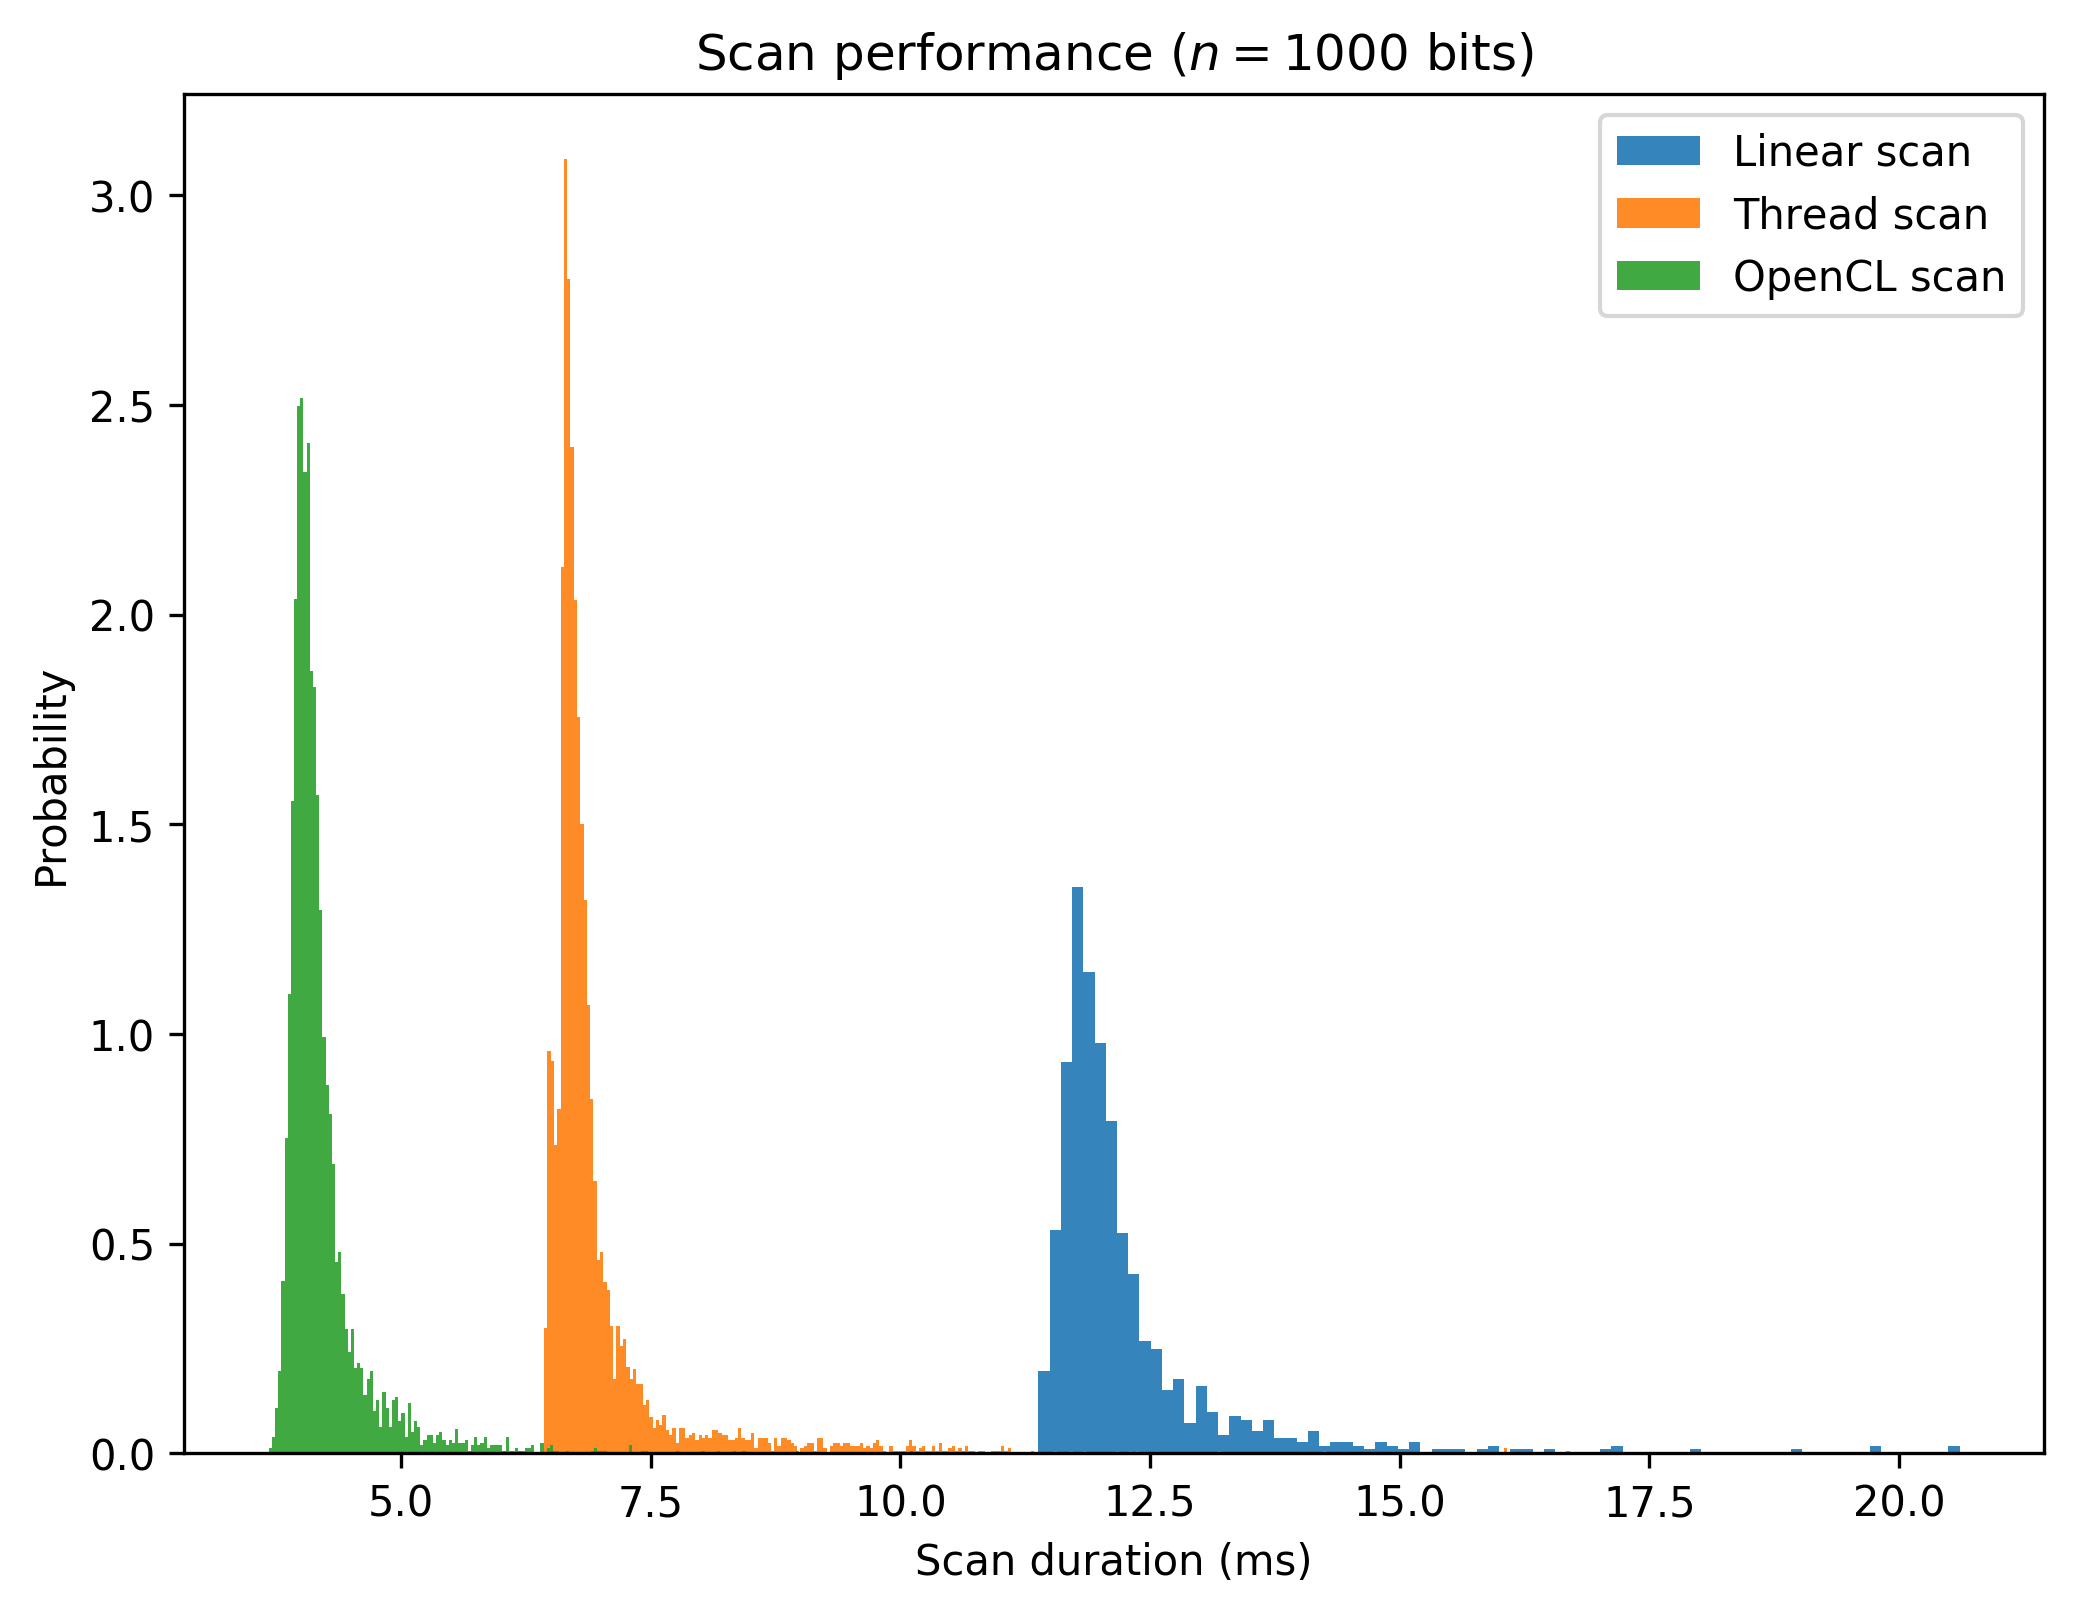
\includegraphics[width=0.7\textwidth]{images02/performance/imac-scan-1000.png}}

\subfloat[$n=10,000$, $r=4805$, and $H=1,000,000$]{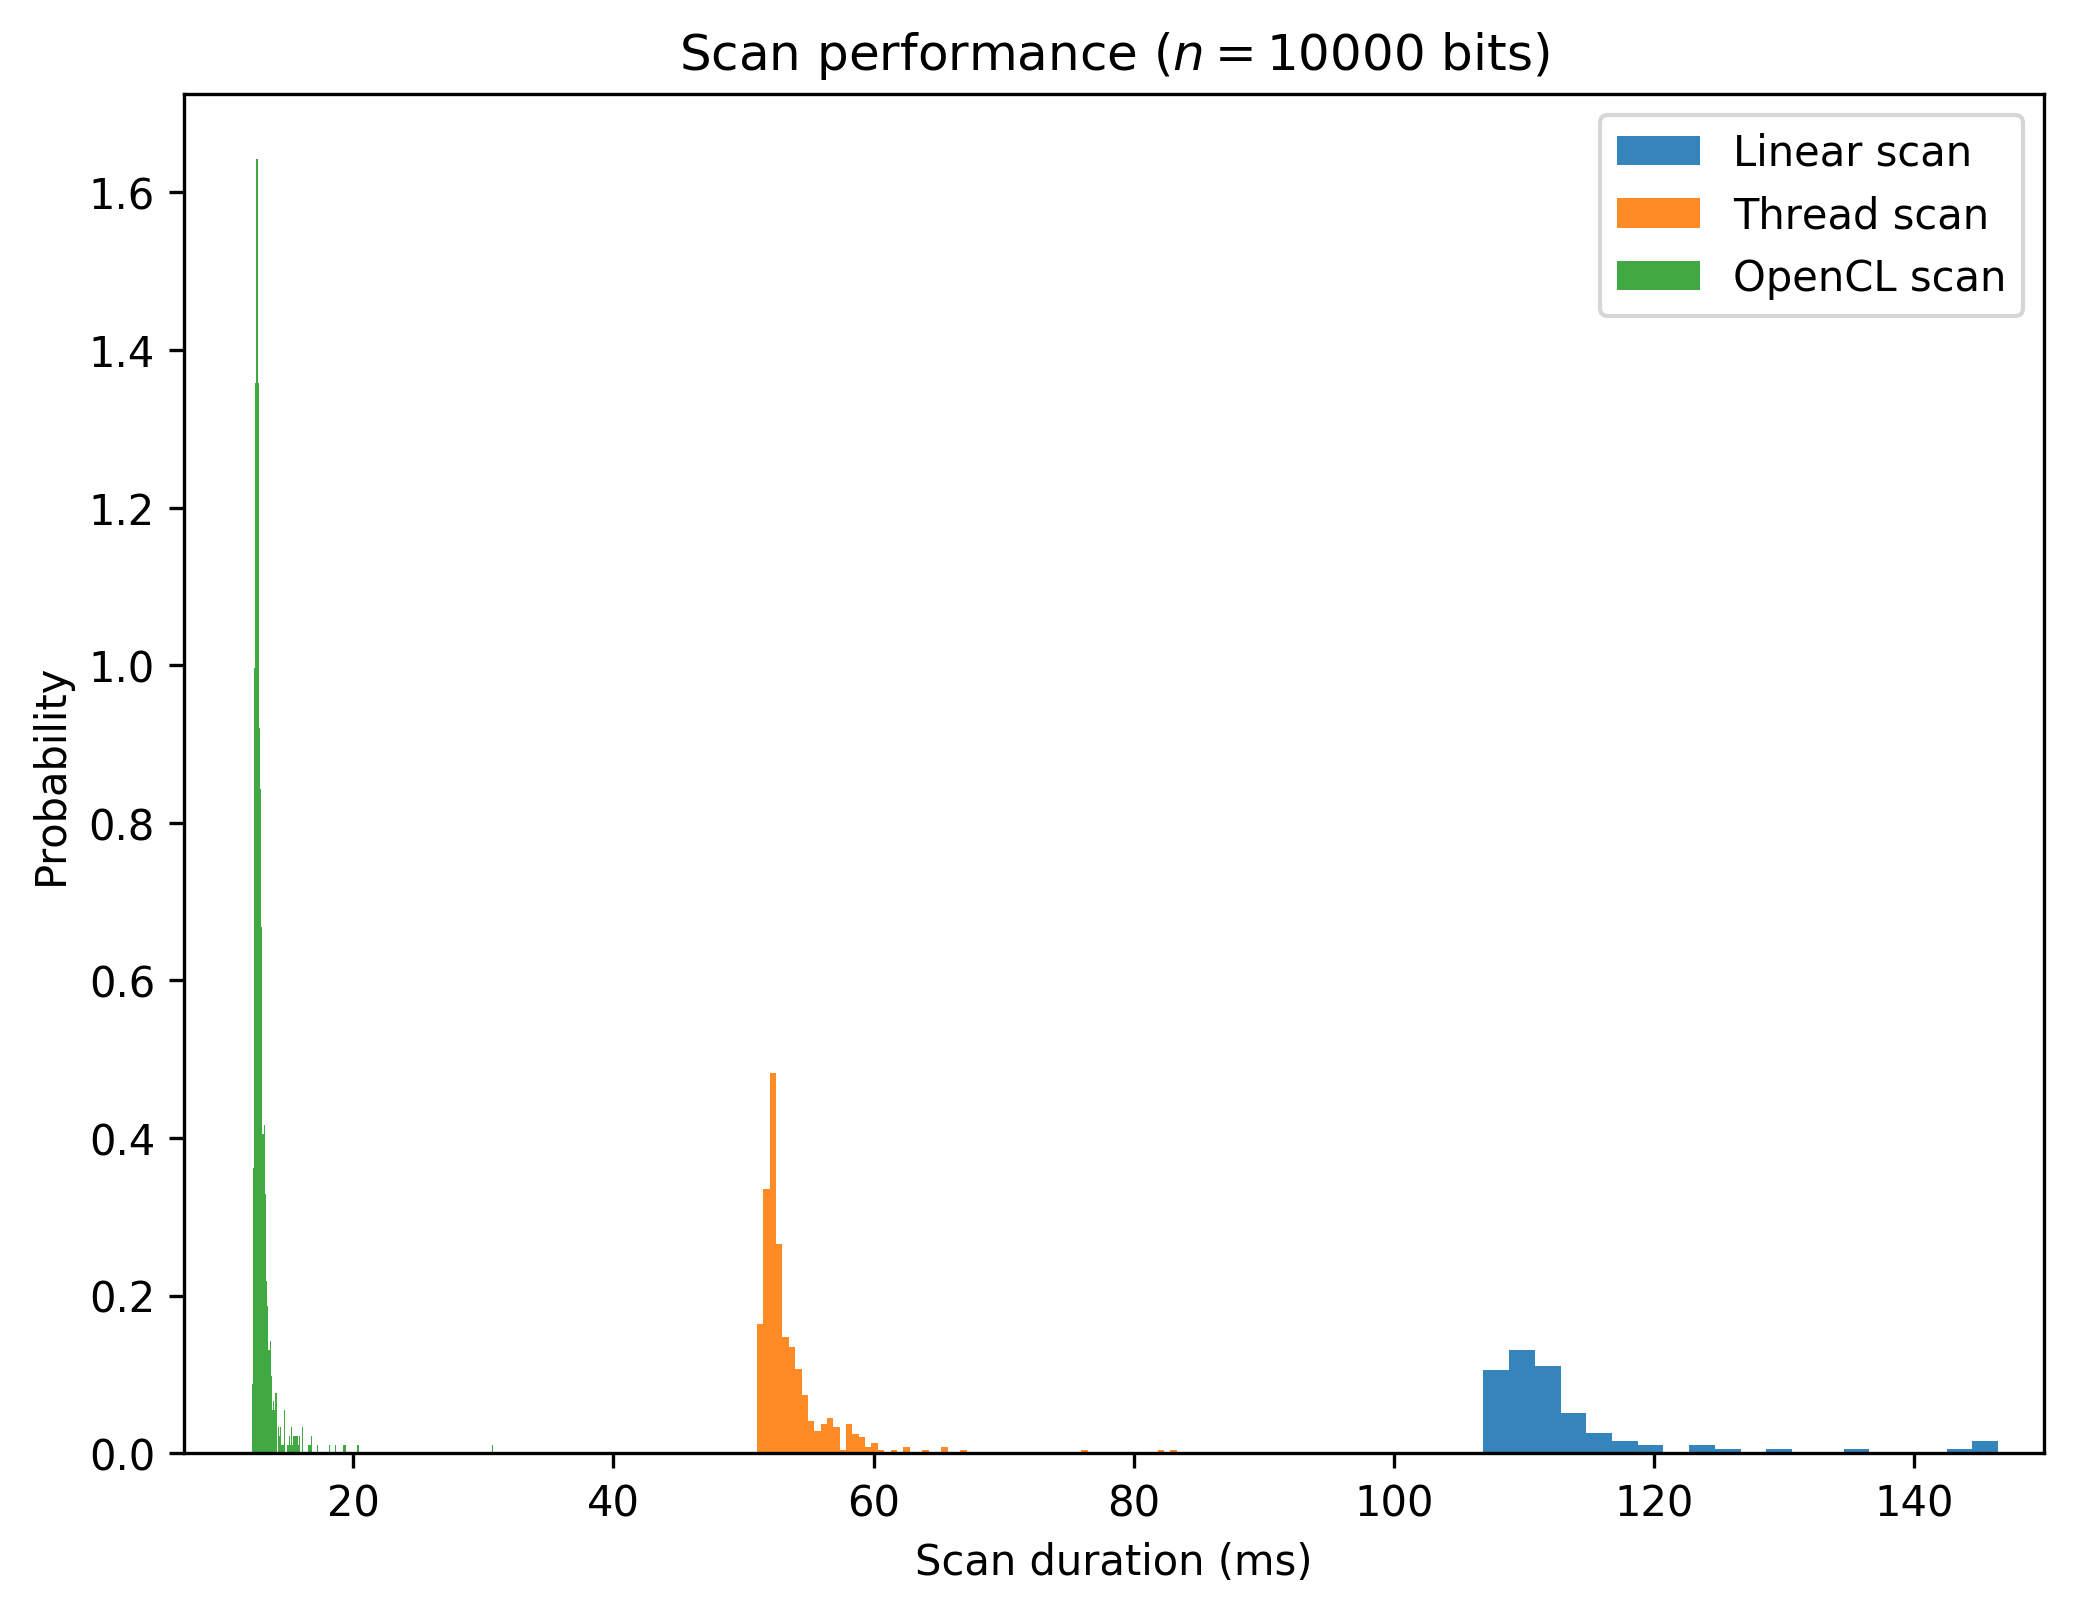
\includegraphics[width=0.7\textwidth]{images02/performance/imac-scan-10k.png}}

\caption{Scanner comparisons for iMac Retina 5K 27-inch 2017 with a 3.8GHz Intel core i5 processor, 8GB DDR4 RAM, and a Radeon Pro 580 8G GPU.
\label{fig:perf-imac-scanners}}
\end{figure}


\begin{figure}[!htb]
\centering
\subfloat[$n=1,000$, $r=451$, and $H=1,000,000$]{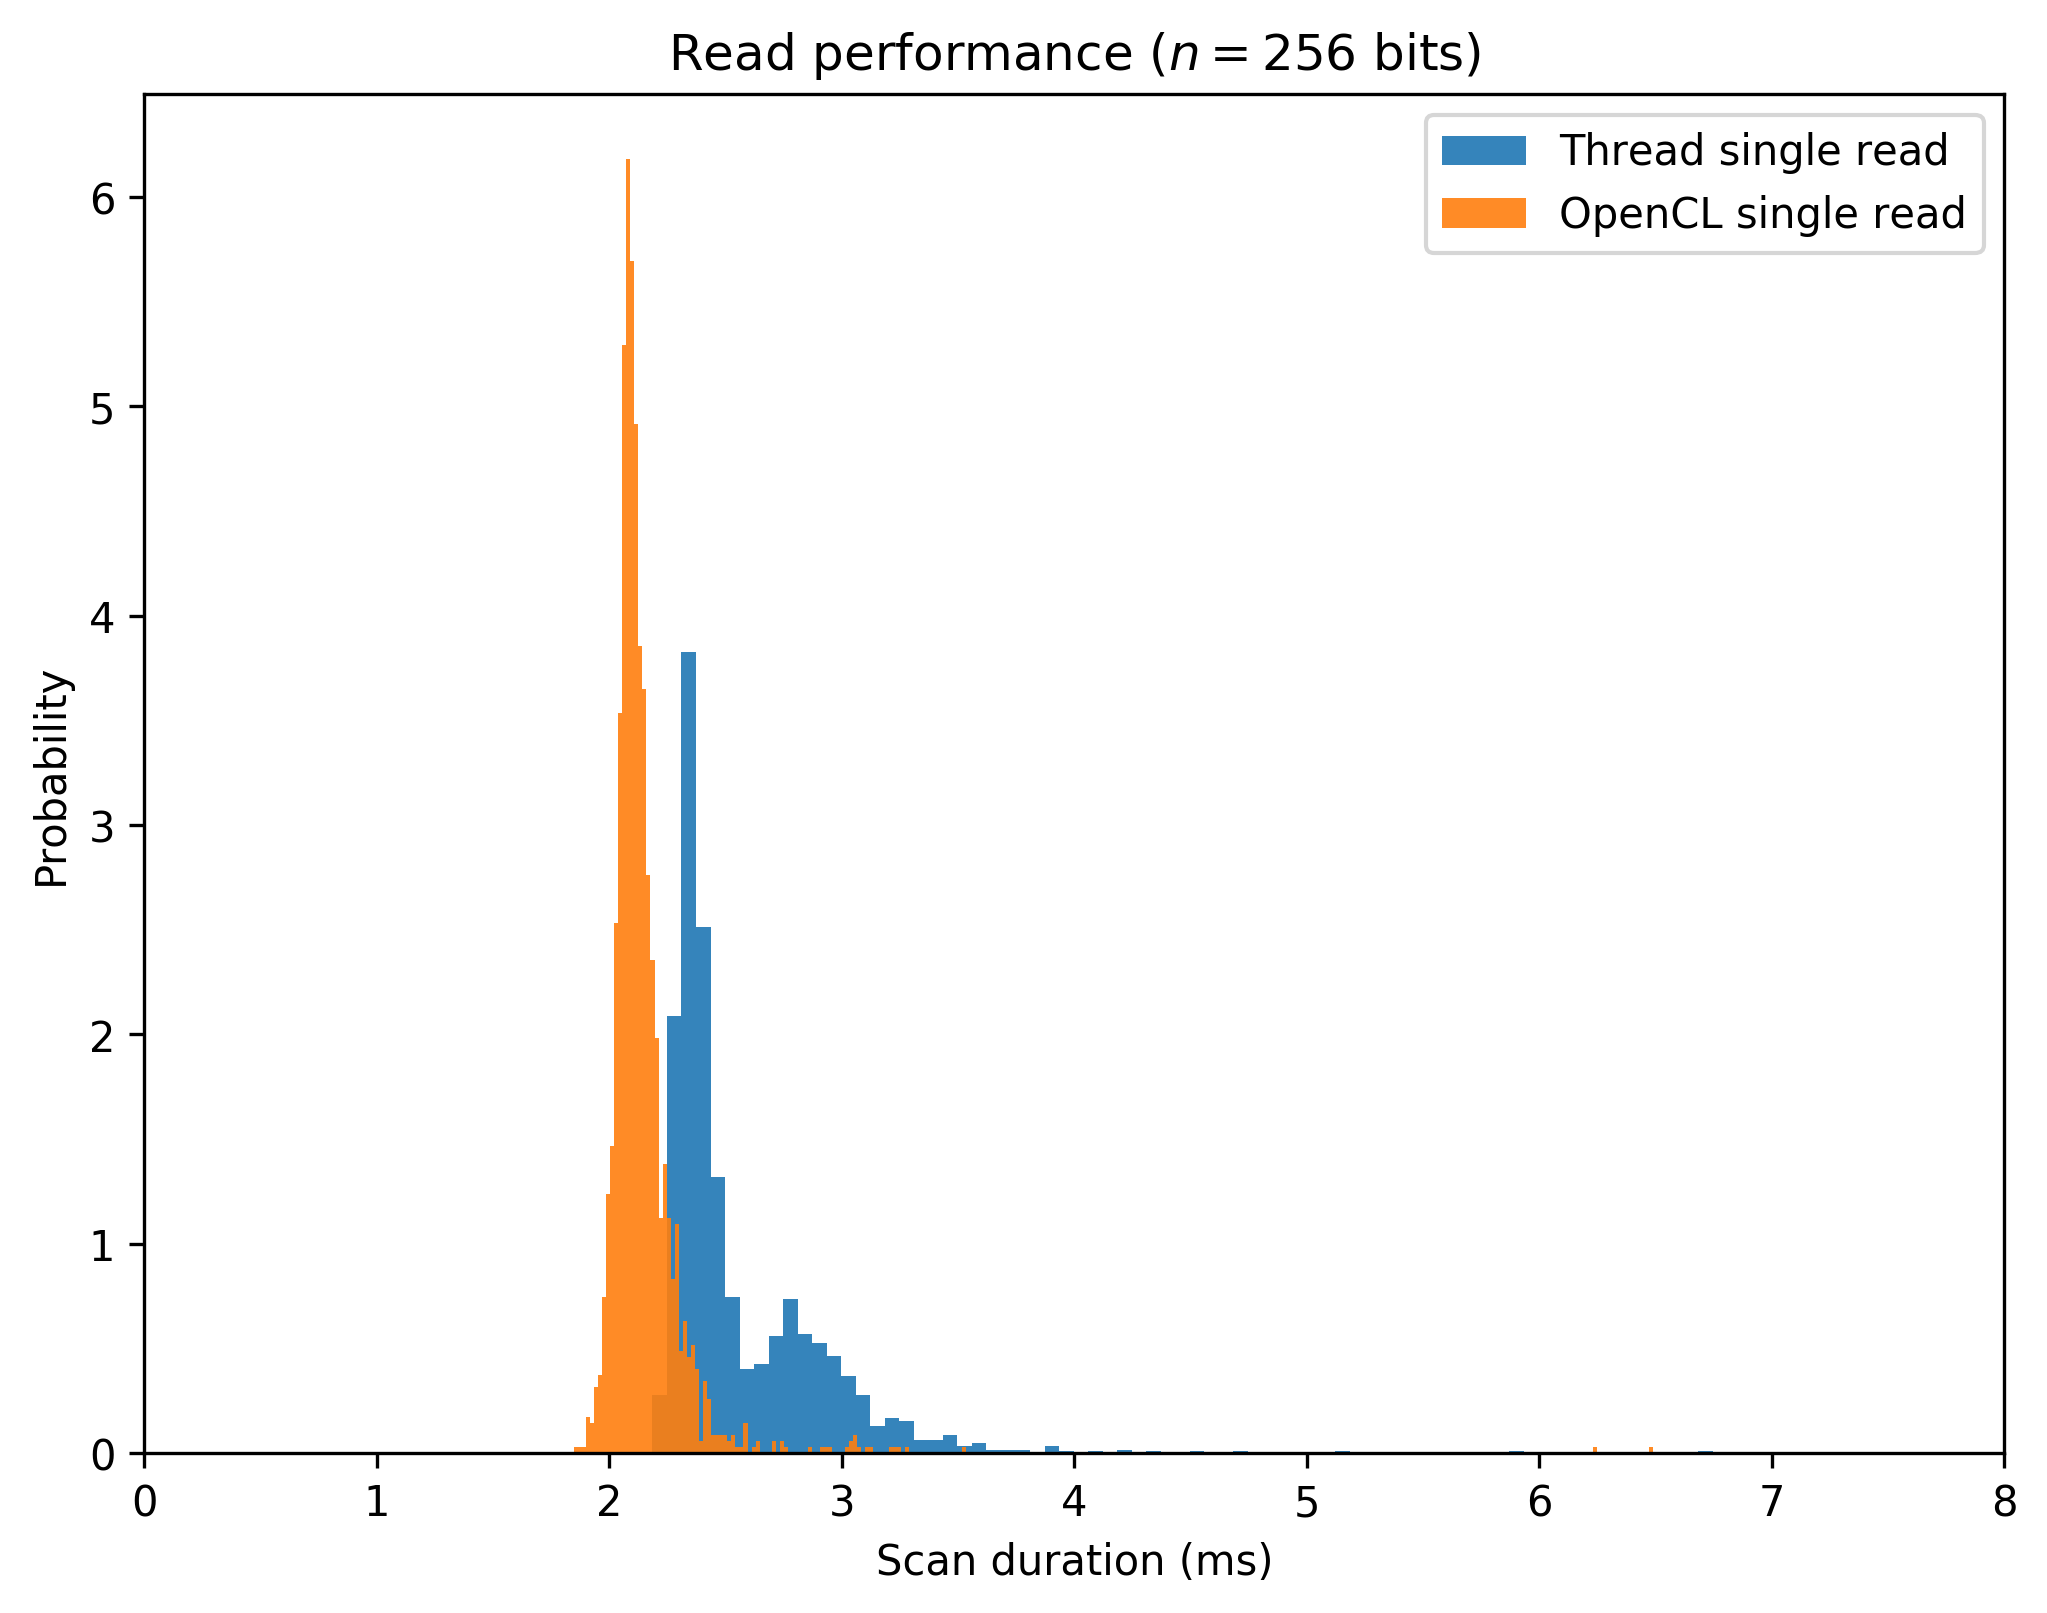
\includegraphics[width=\textwidth]{images02/performance/imac-read-256.png}}

\subfloat[$n=1,000$, $r=451$, and $H=1,000,000$]{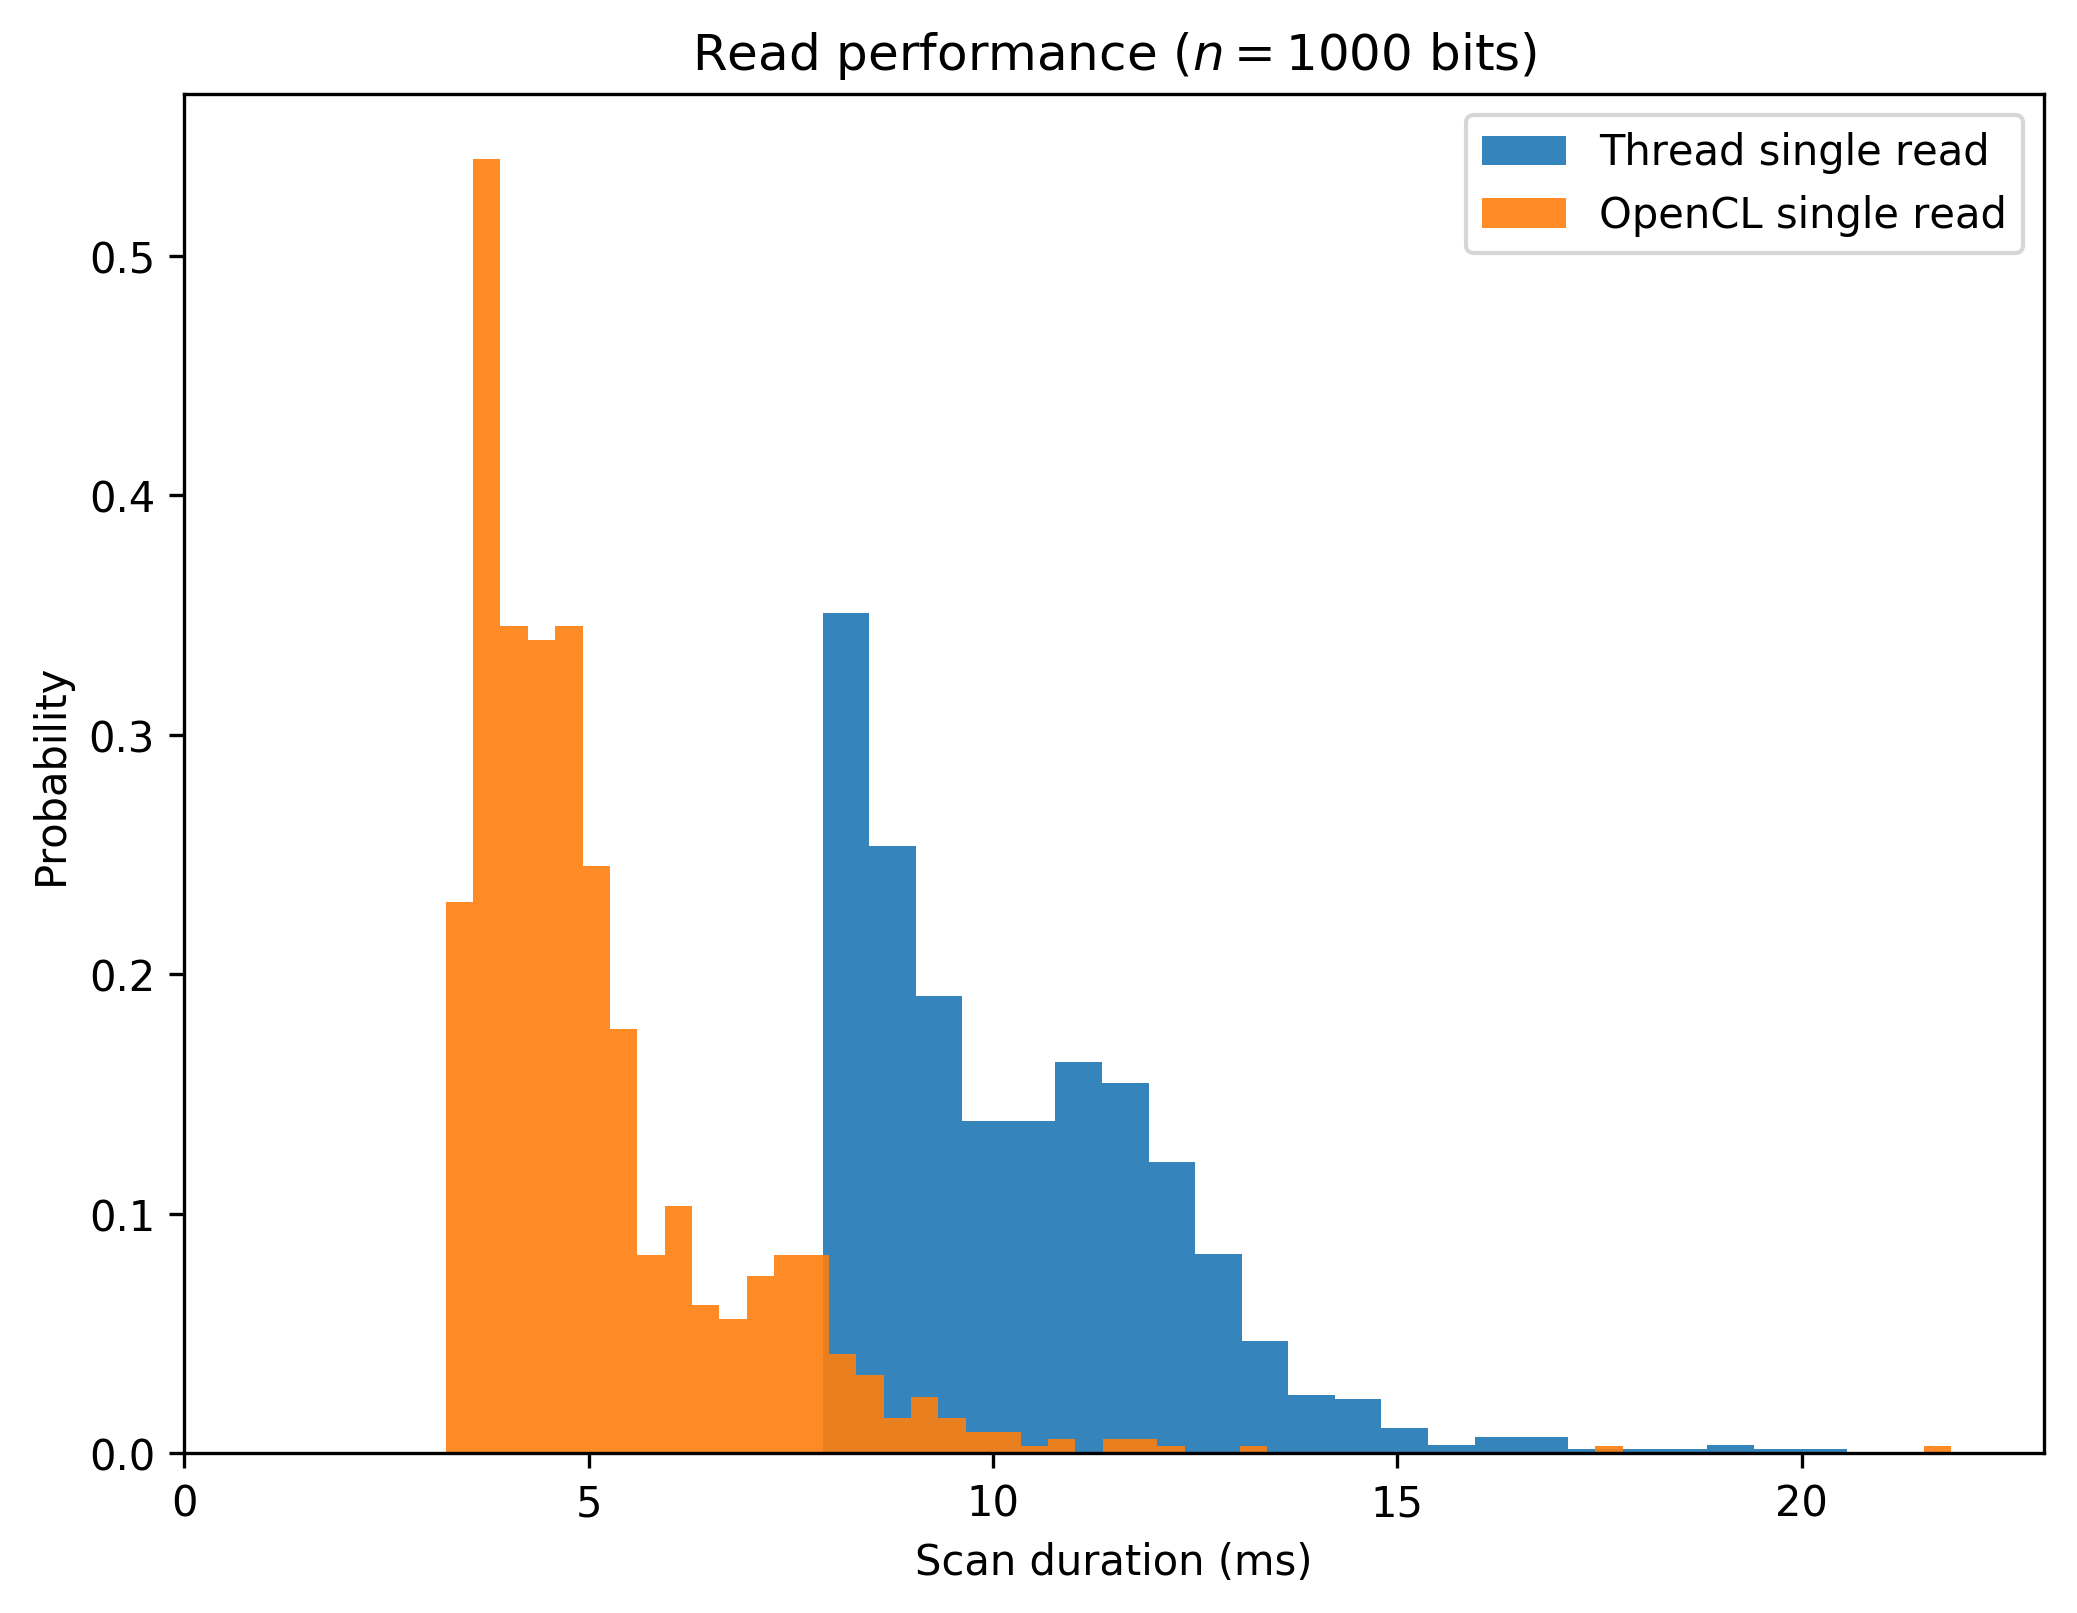
\includegraphics[width=\textwidth]{images02/performance/imac-read-1000.png}}

\caption{Read operation comparisons for iMac Retina 5K 27-inch 2017 with a 3.8GHz Intel core i5 processor, 8GB DDR4 RAM, and a Radeon Pro 580 8G GPU.
\label{fig:perf-imac-read}}
\end{figure}

\begin{figure}[!htb]
\centering
\subfloat[$n=1,000$, $r=451$, and $H=1,000,000$]{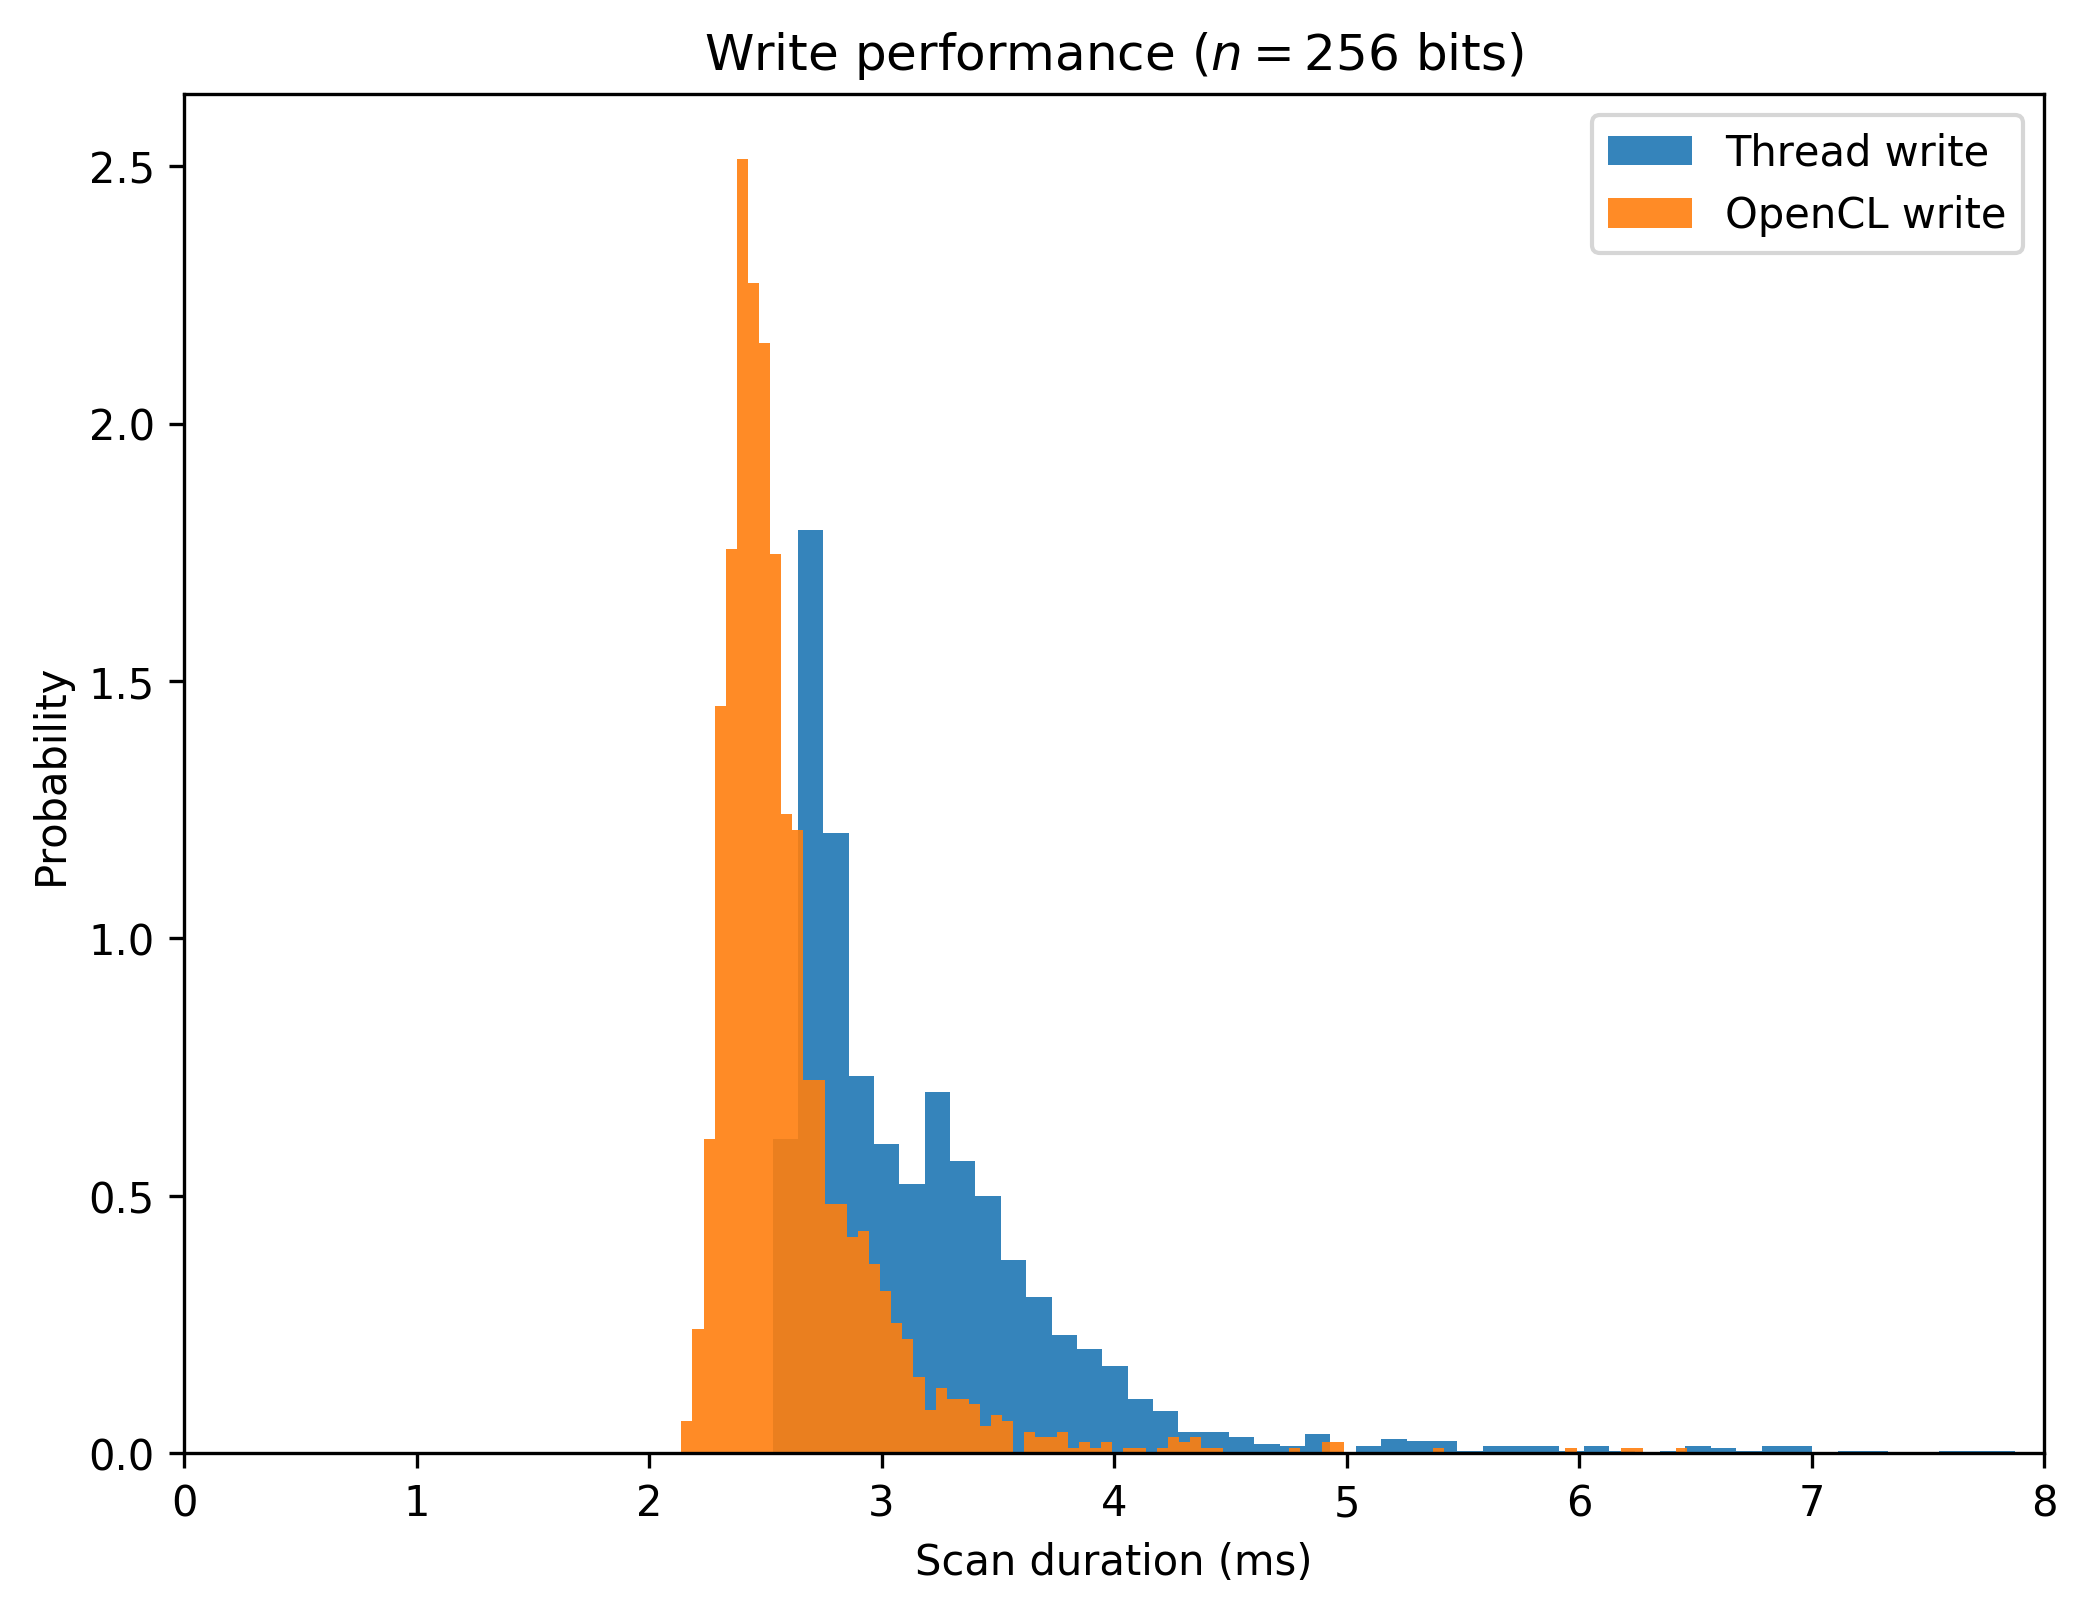
\includegraphics[width=\textwidth]{images02/performance/imac-write-256.png}}

\subfloat[$n=1,000$, $r=451$, and $H=1,000,000$]{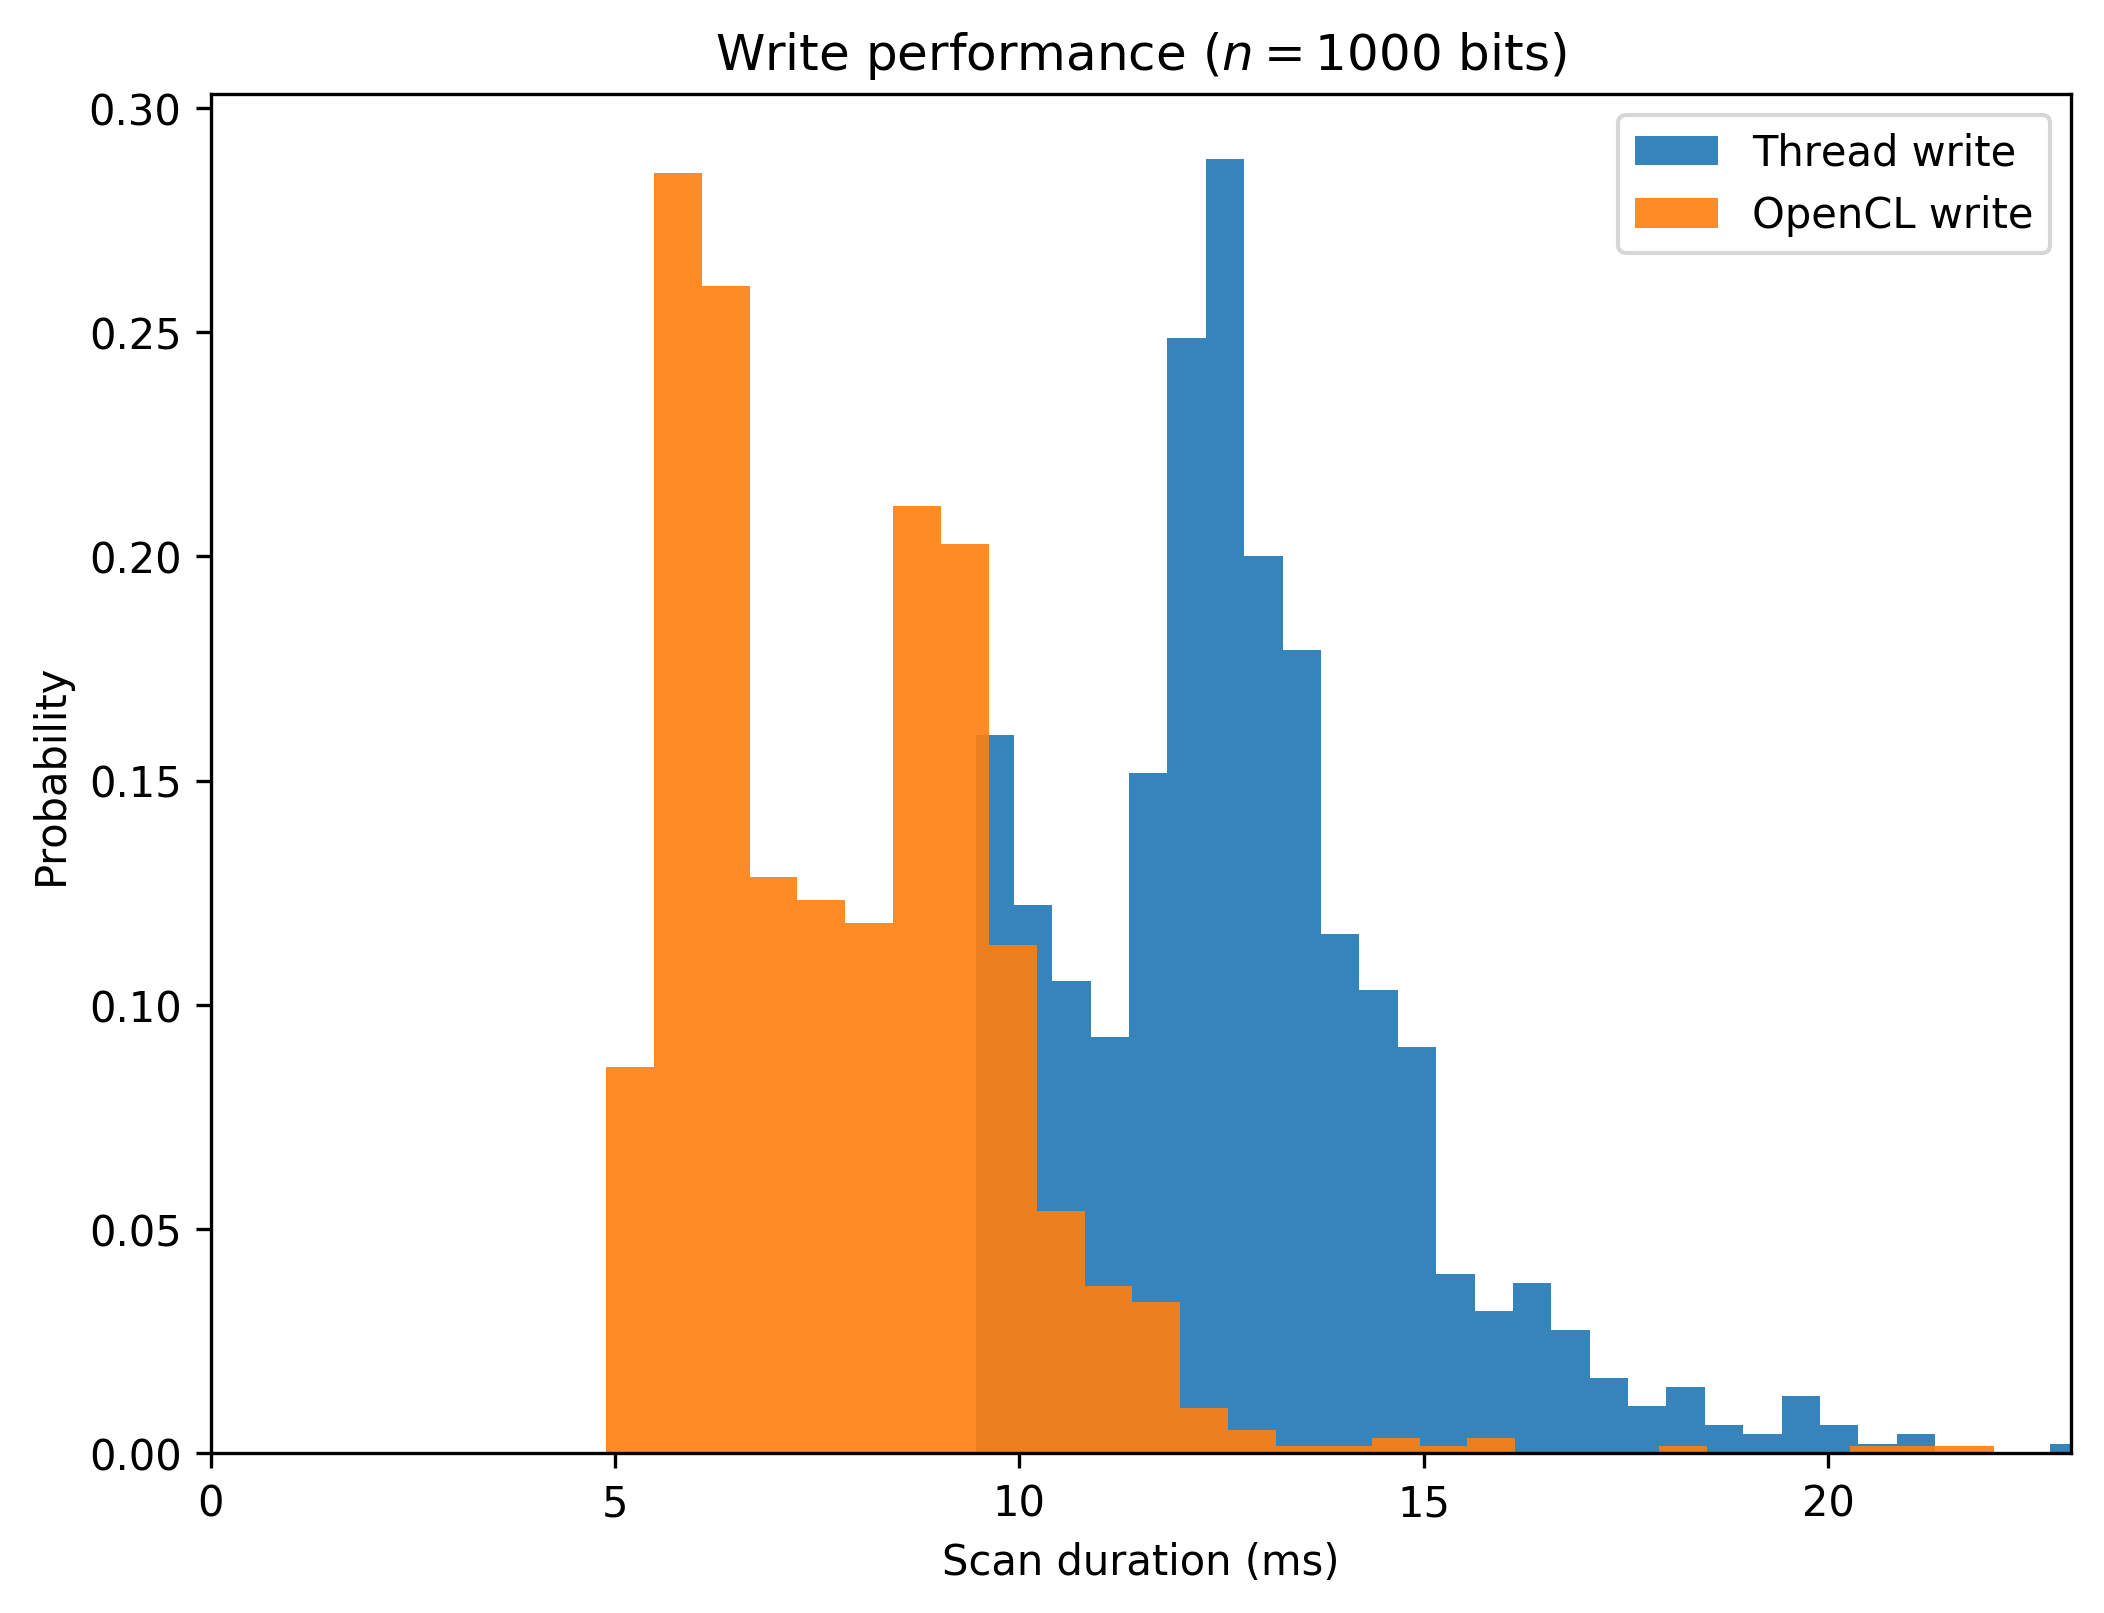
\includegraphics[width=\textwidth]{images02/performance/imac-write-1000.png}}

\caption{Write operation comparisons for iMac Retina 5K 27-inch 2017 with a 3.8GHz Intel core i5 processor, 8GB DDR4 RAM, and a Radeon Pro 580 8G GPU.
\label{fig:perf-imac-write}}
\end{figure}




% -------------------------
% -------------------------
% -------------------------



\begin{table}[!htb]
\centering
\begin{tabular}{lrrr}
    \toprule
    & \textbf{256 bits} & \textbf{1,000 bits} & \textbf{10,000 bits} \\ \hline
	\hline
	Kernels & Duration (ms) & Duration (ms) & Duration (ms) \\ \hline
    single\_scan0 &  0.76 &  3.79 & 35.45 \\
    single\_scan1 &  0.80 &  3.94 & 57.80 \\
    single\_scan2 &  5.59 &  8.54 & 63.71 \\
    single\_scan3 &  6.31 &  9.73 & 39.92 \\
    single\_scan4 & 10.29 & 11.38 & 45.49 \\
    single\_scan5 &  6.69 &  9.95 & 43.51 \\
	single\_scan5\_unroll & & & \\
    single\_scan6 & 10.29 & 11.33 & 41.42 \\
    \hline
	Scanners & Duration (ms) & Duration (ms) & Duration (ms) \\ \hline
    Linear scan & 19.09 & 64.73 & 600.75 \\
    Thread scan &  9.95 & 32.81 & 296.56 \\
    OpenCL scan &  6.88 & 10.67 &  46.73 \\ \hline
    \hline
	Operations & Duration (ms) & Duration (ms) & Duration (ms) \\ \hline
    Thread write       & 11.80 & 42.64 & 383.50 \\
    Thread single read & 10.49 & 35.37 & 307.97 \\
    OpenCL write       &  8.84 & 19.31 & 122.17 \\
    OpenCL single read &  7.50 & 11.72 &  55.47 \\
    \bottomrule
\end{tabular}
\caption{Amazon EC2 p2.xlarge with Intel Xeon E5-2686v4 processor, 61GB DDR3 RAM, and NVIDIA K80 GPU. Running an SDM with $n=256$ bits, $H=1,000,000$, and $r=103$. The SDM settings were: (i) $n=256$, $r=103$, and $H=1,000,000$; (ii) $n=1,000$, $r=451$, and $H=1,000,000$; and (iii) $n=10,000$, $r=4850$, and $H=1,000,000$. There is no benchmark for kernel single\_scan5\_unroll because it returns the wrong result in this GPU. The problem is related to the premises of the optimization used by this kernel, which are not true for this GPU.
For the histogram of durations, see Figures \ref{fig:perf-ec2-p2-kernels}, \ref{fig:perf-imac-scanners}, \ref{fig:perf-imac-read}, and \ref{fig:perf-imac-write}.
\label{tab:perf-ec2-p2}}
\end{table}


\begin{figure}[!htb]
\centering
\subfloat[$n=256$, $r=103$, and $H=1,000,000$]{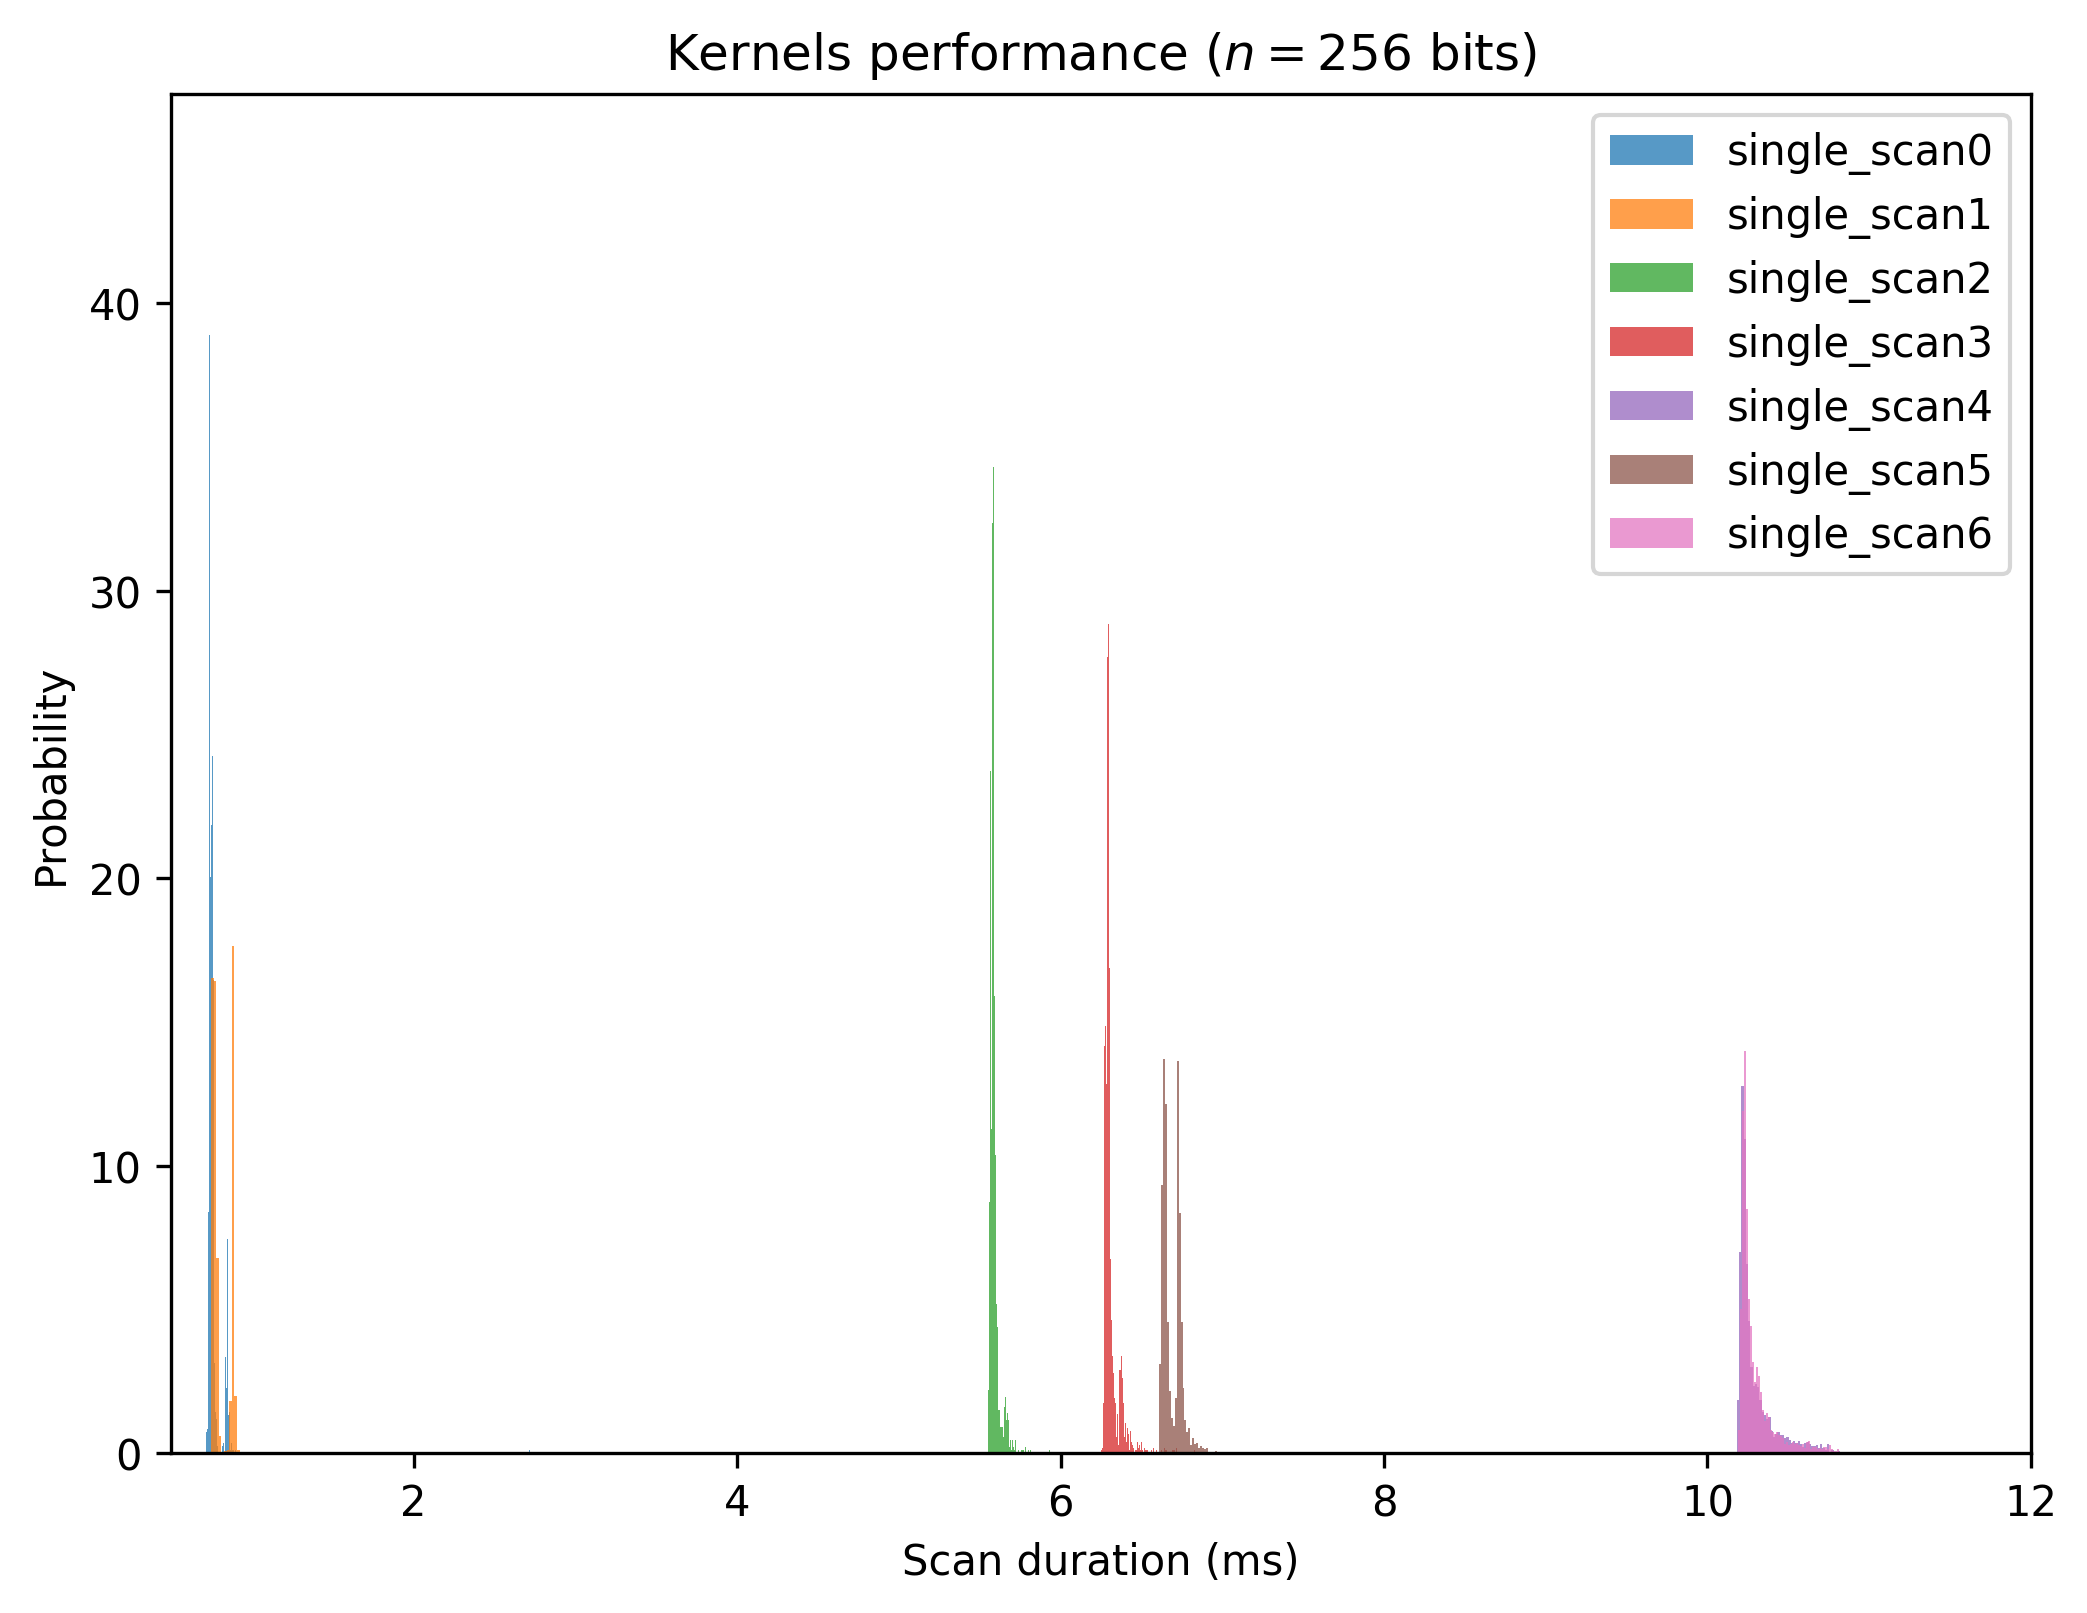
\includegraphics[width=0.7\textwidth]{images02/performance/ec2-p2-kernels-256.png}}

\subfloat[$n=1,000$, $r=451$, and $H=1,000,000$]{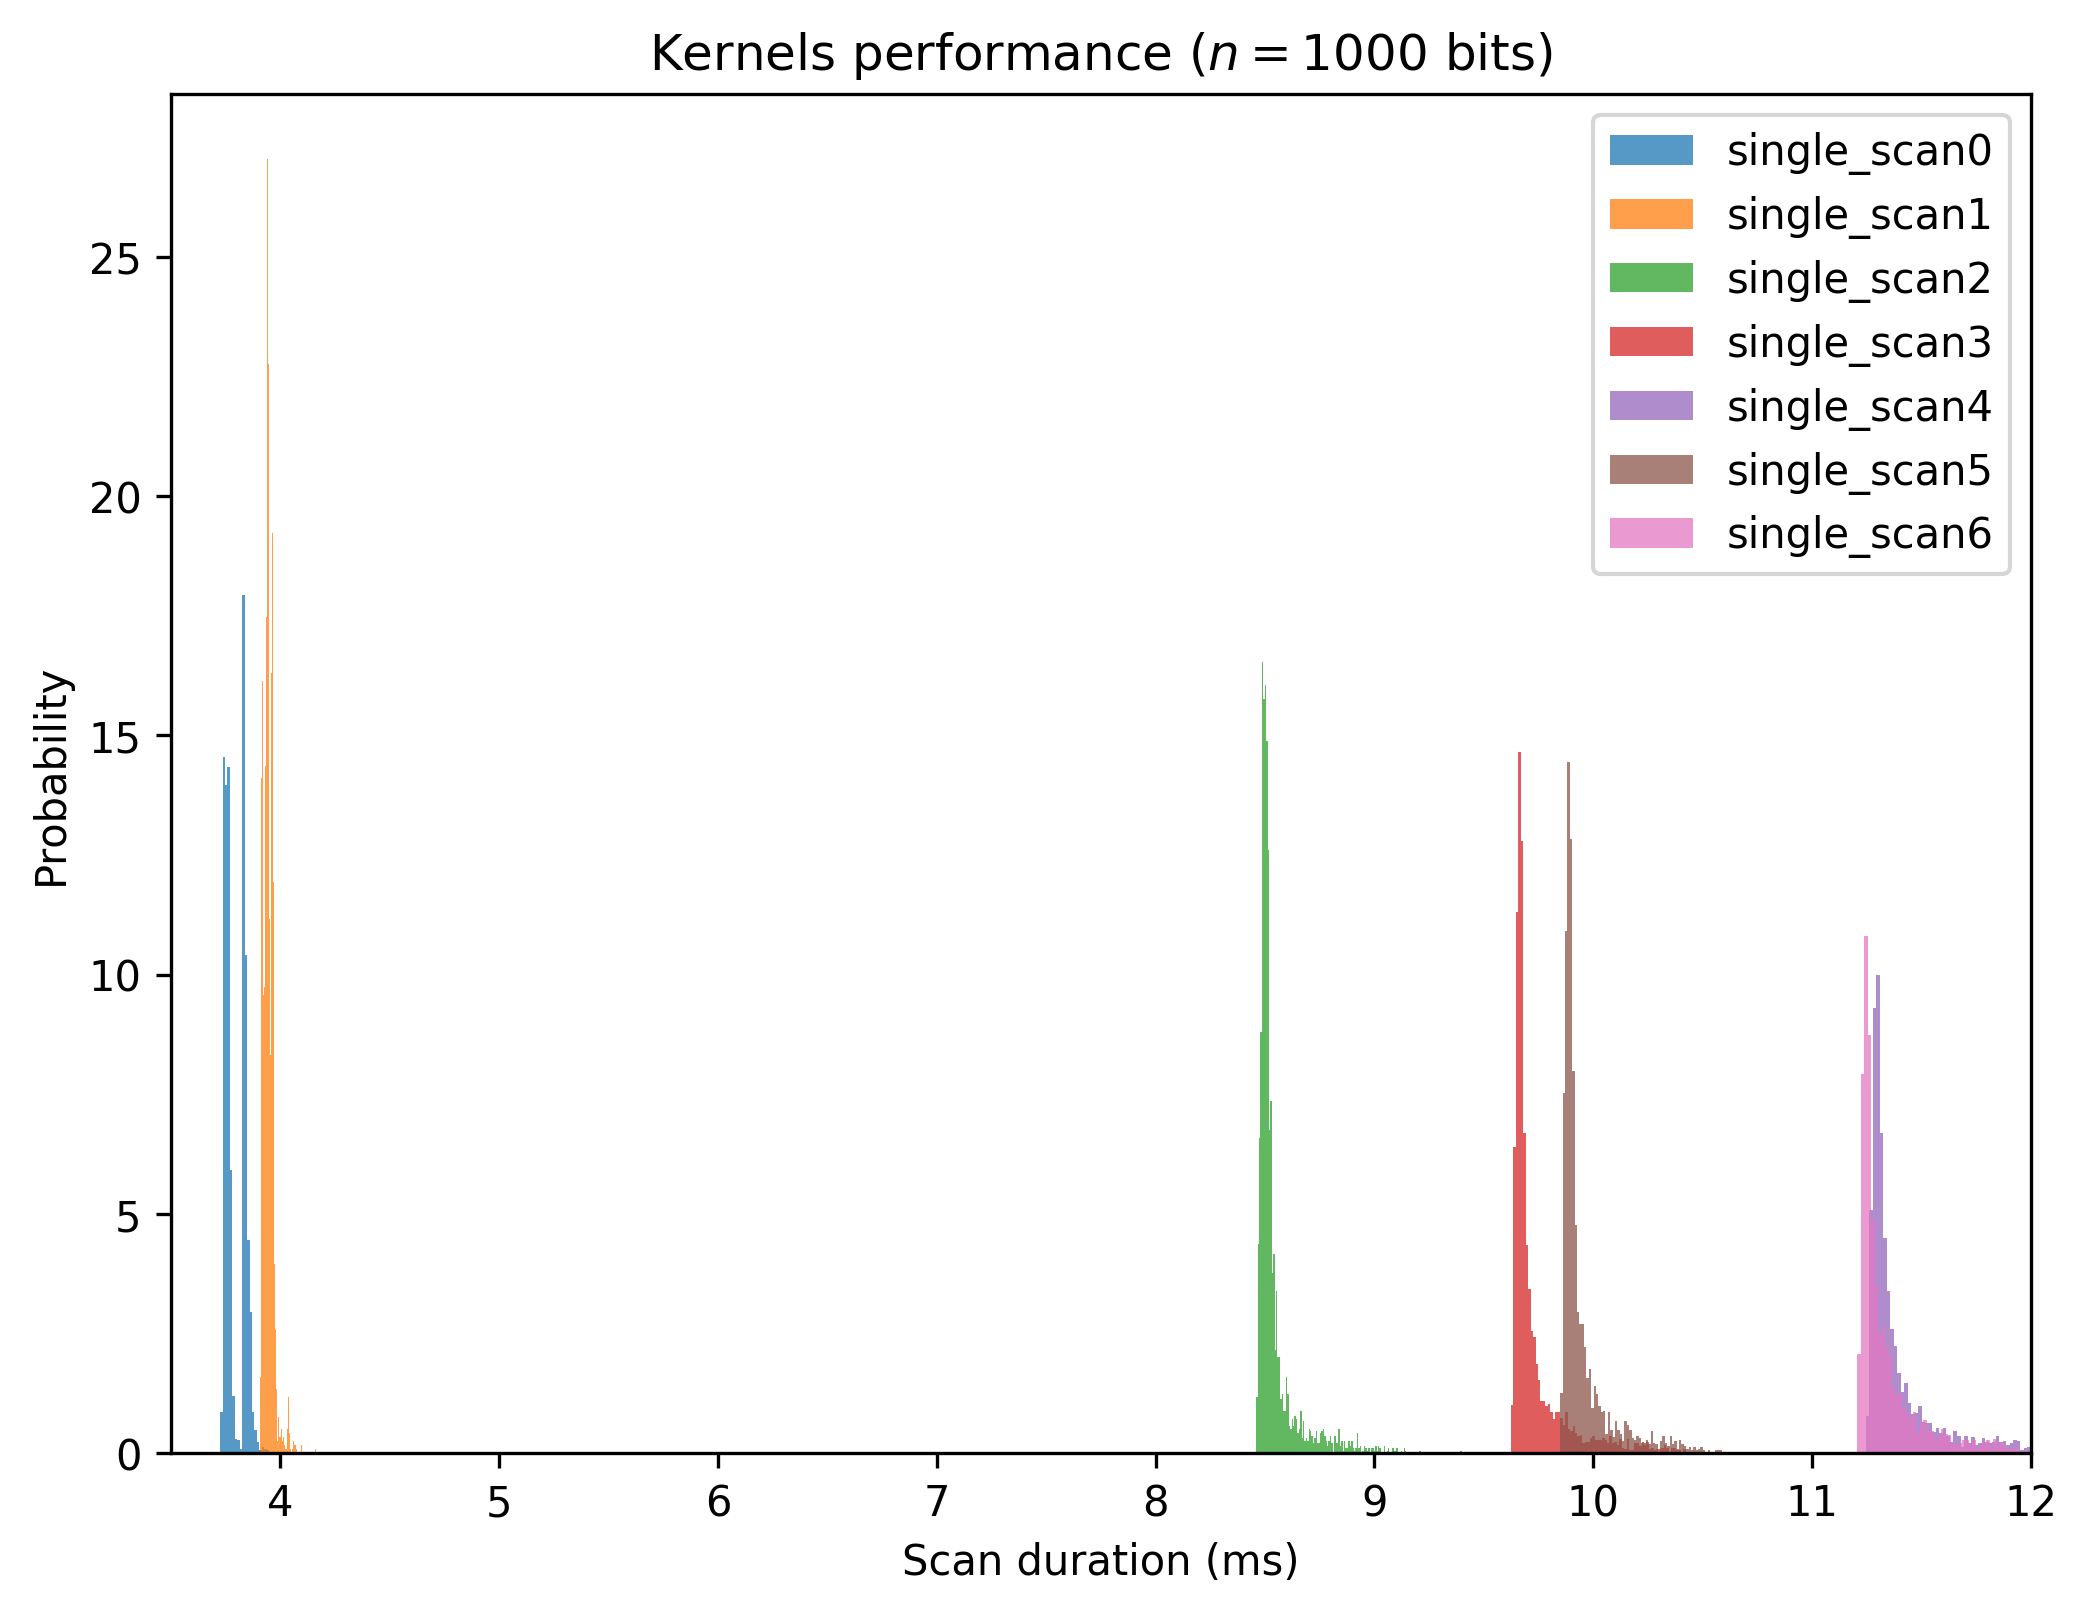
\includegraphics[width=0.7\textwidth]{images02/performance/ec2-p2-kernels-1000.png}}

\subfloat[$n=10,000$, $r=4805$, and $H=1,000,000$]{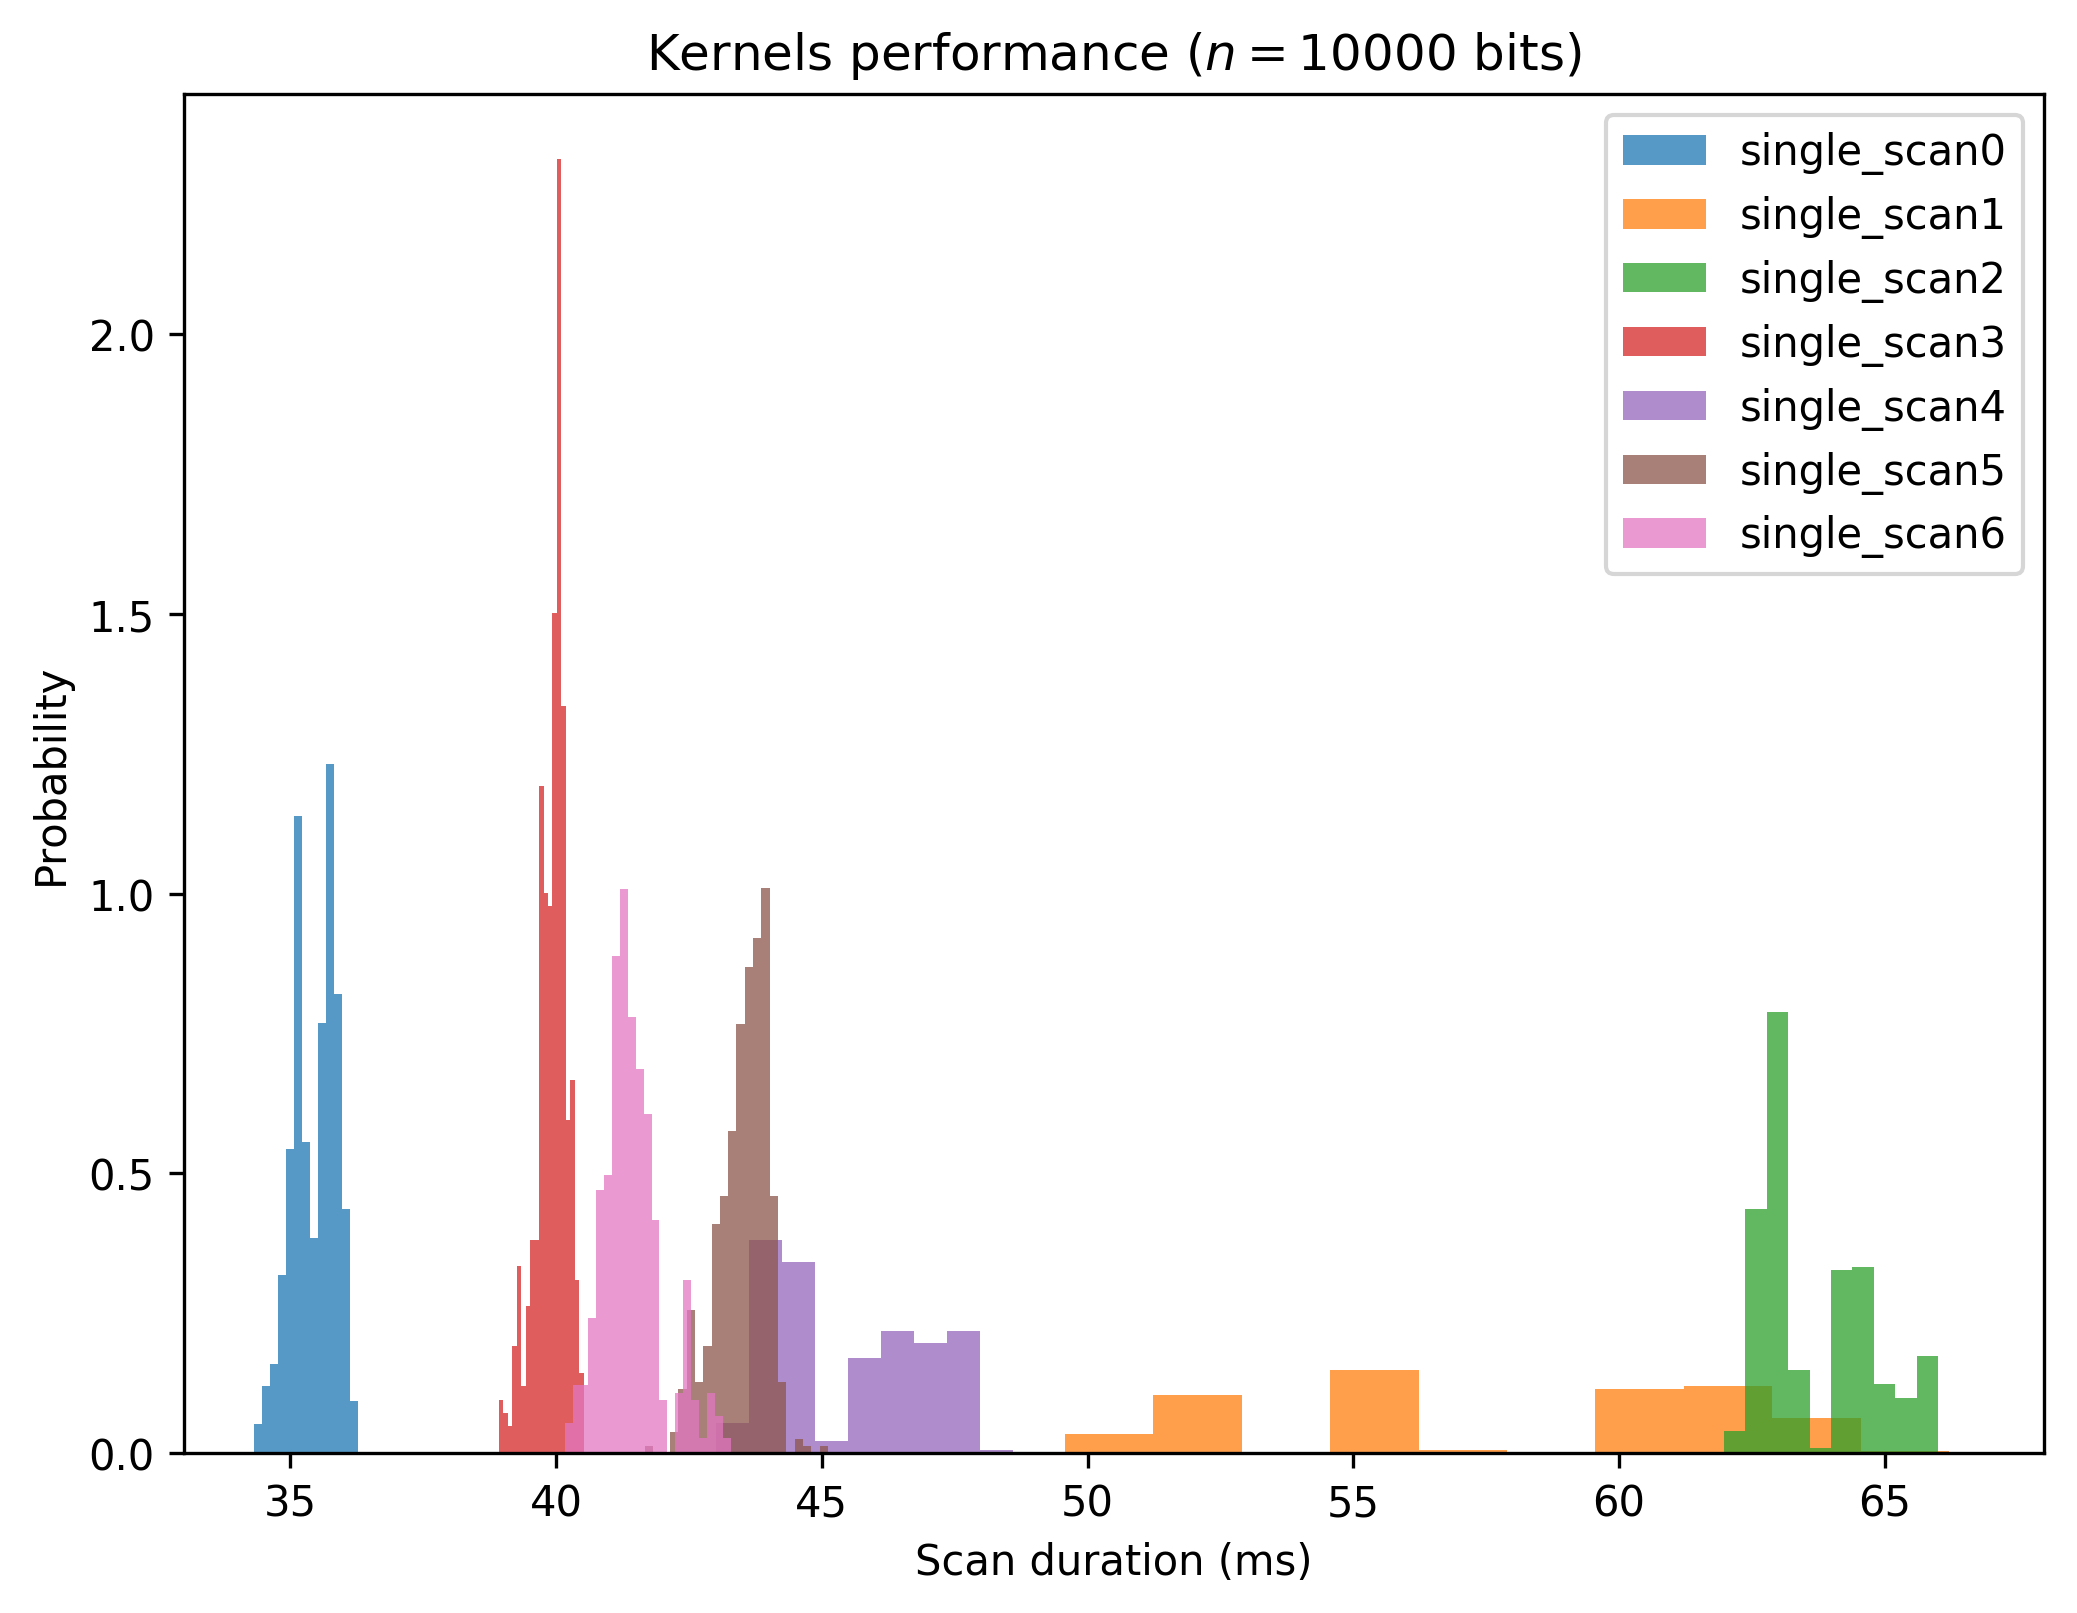
\includegraphics[width=0.7\textwidth]{images02/performance/ec2-p2-kernels-10k.png}}

\caption{Kernel comparisons for Amazon EC2 p2.xlarge with Intel Xeon E5-2686v4 processor, 61GB DDR3 RAM, and NVIDIA K80 GPU.
\label{fig:perf-ec2-p2-kernels}}
\end{figure}

\begin{figure}[!htb]
\centering
\subfloat[$n=1,000$, $r=451$, and $H=1,000,000$]{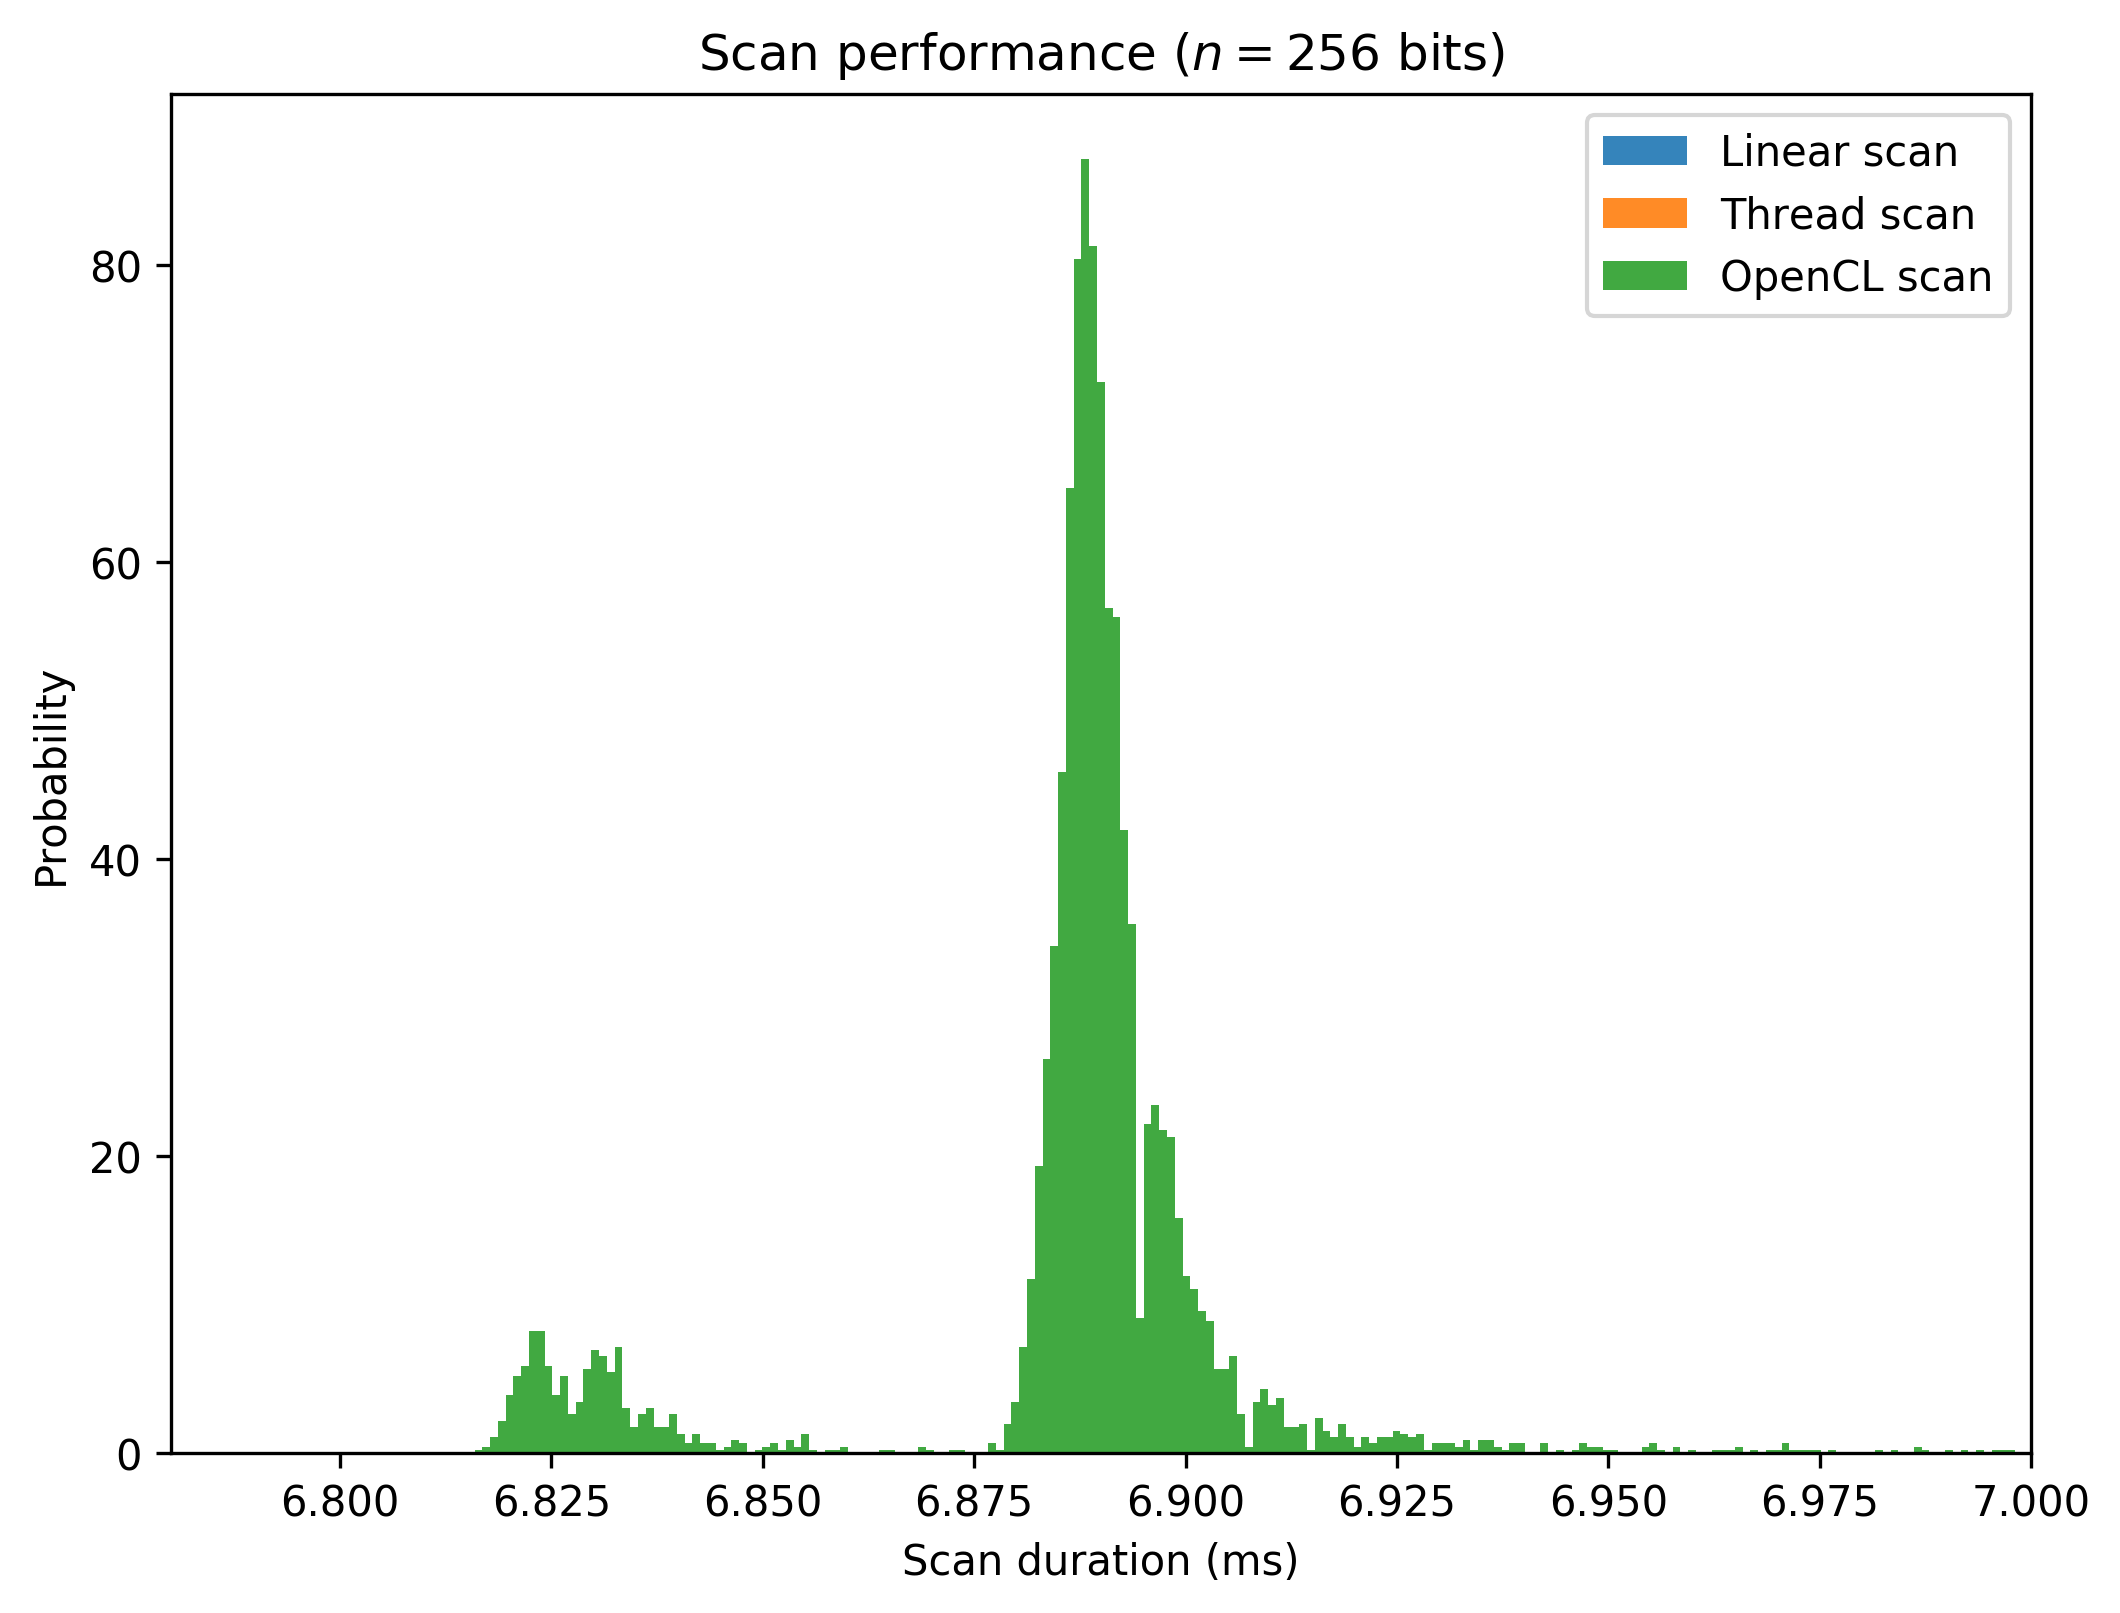
\includegraphics[width=0.7\textwidth]{images02/performance/ec2-p2-scan-256.png}}

\subfloat[$n=1,000$, $r=451$, and $H=1,000,000$]{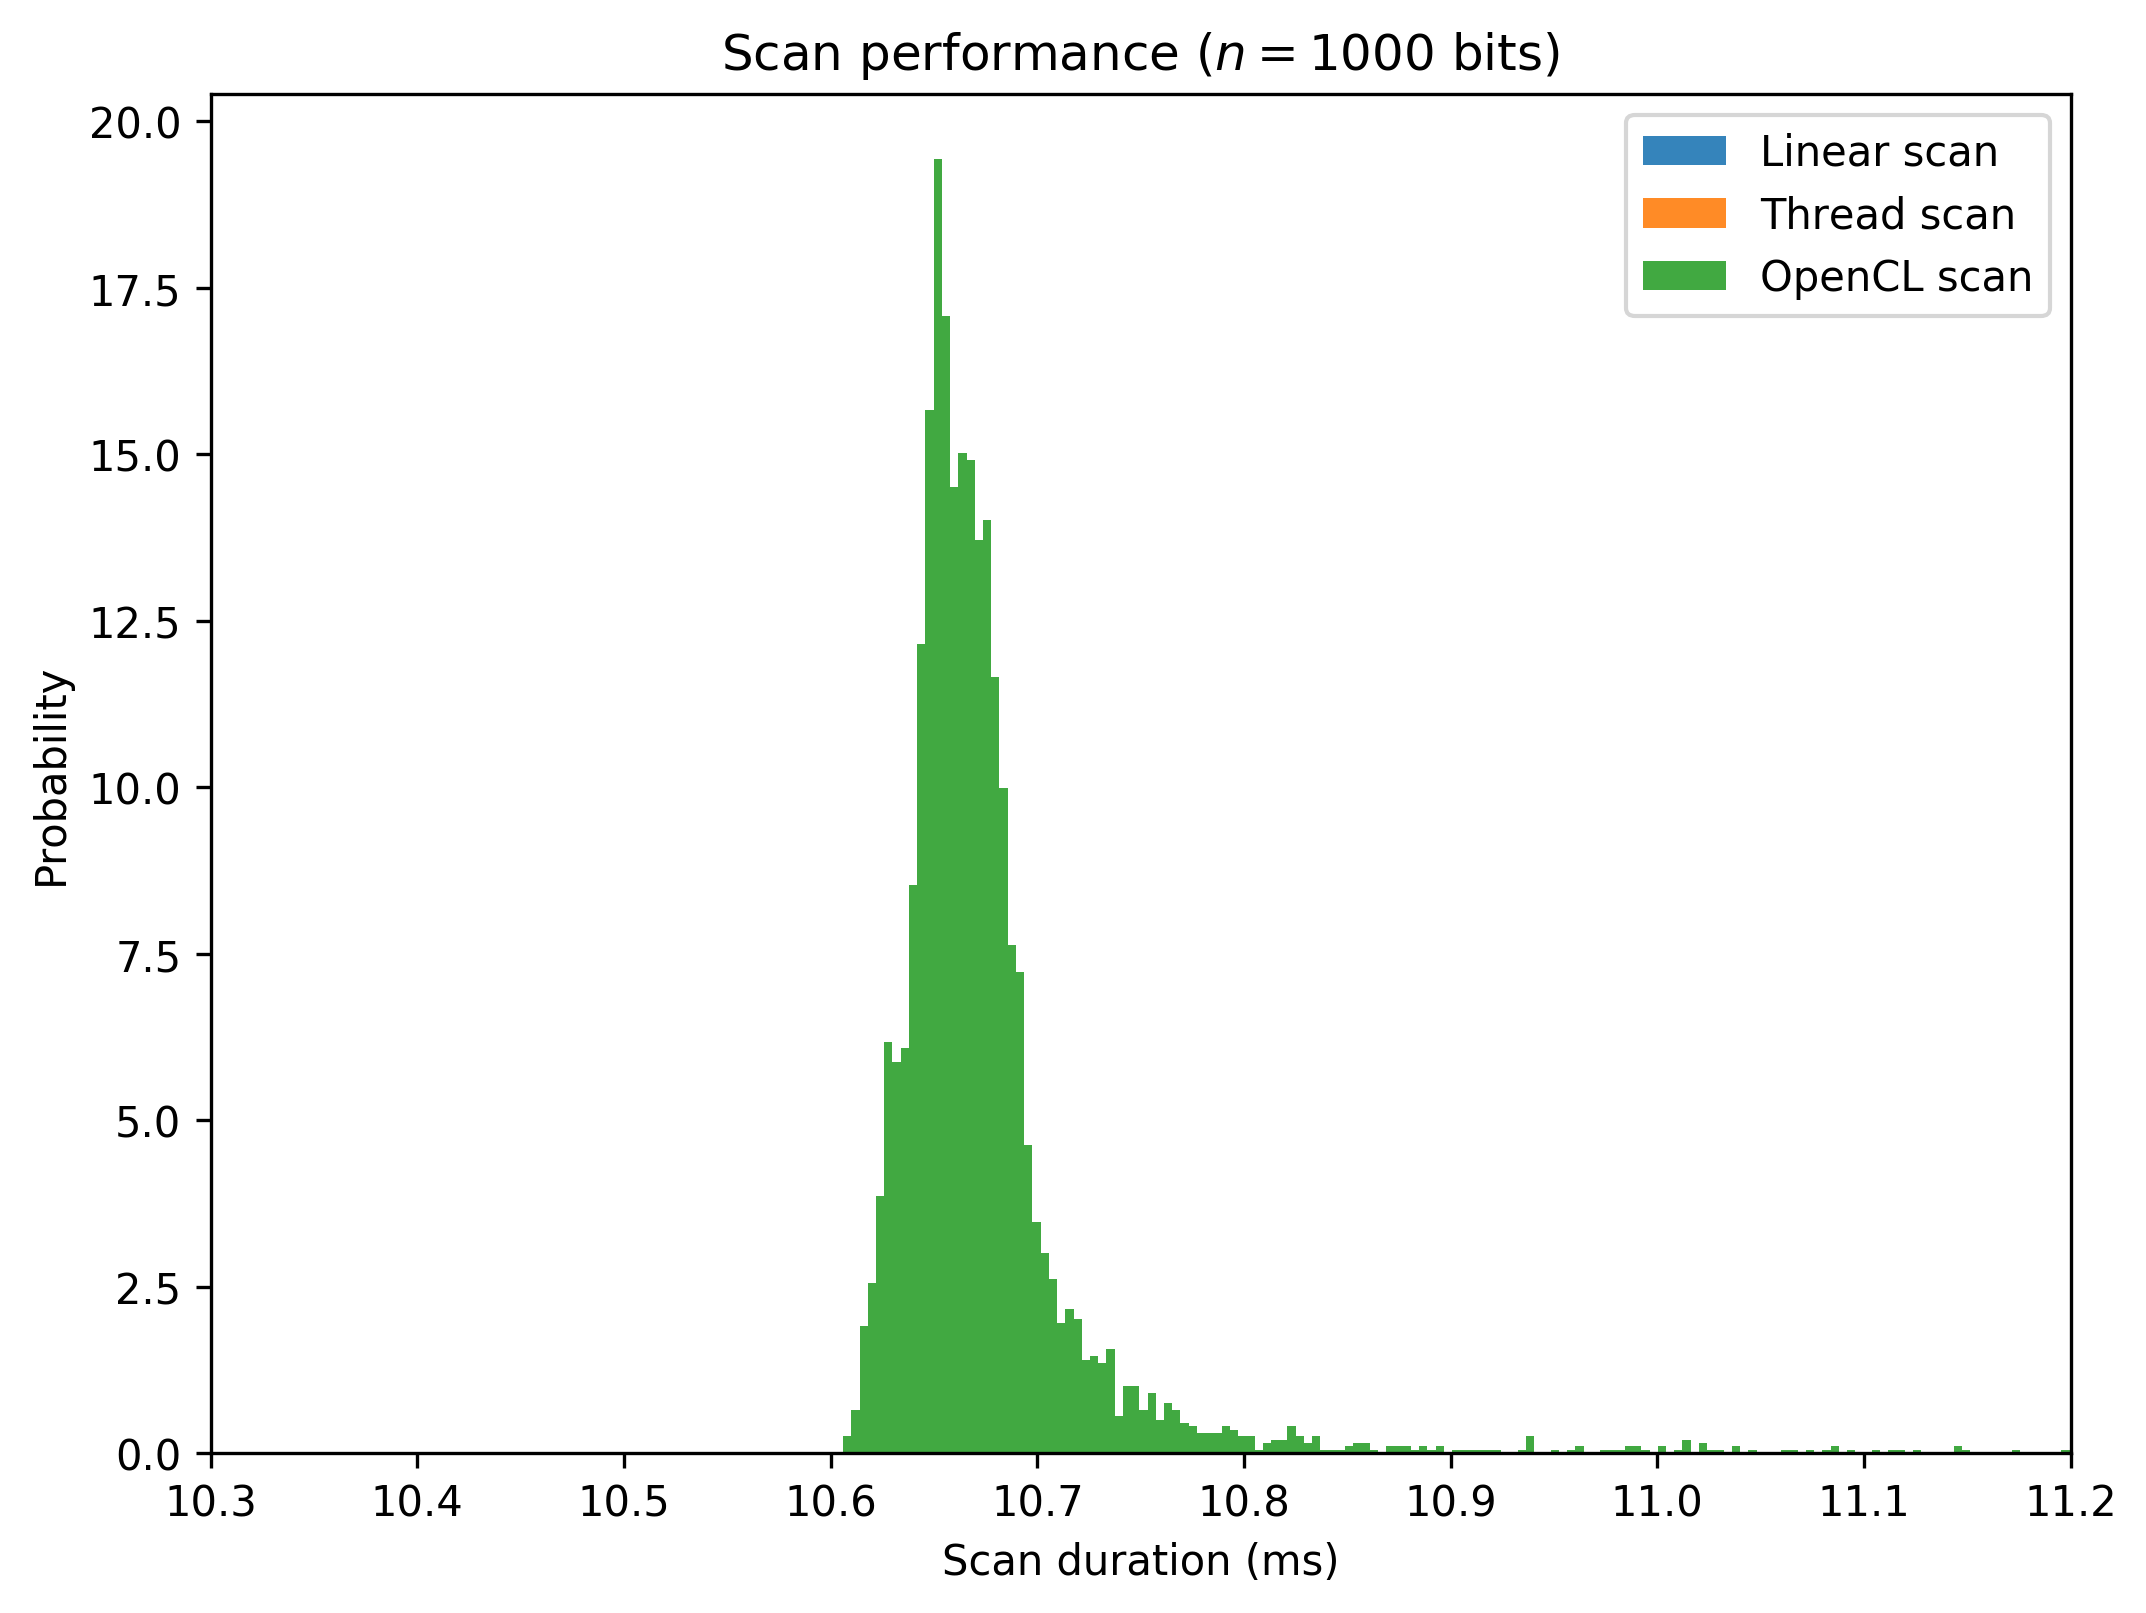
\includegraphics[width=0.7\textwidth]{images02/performance/ec2-p2-scan-1000.png}}

\subfloat[$n=10,000$, $r=4805$, and $H=1,000,000$]{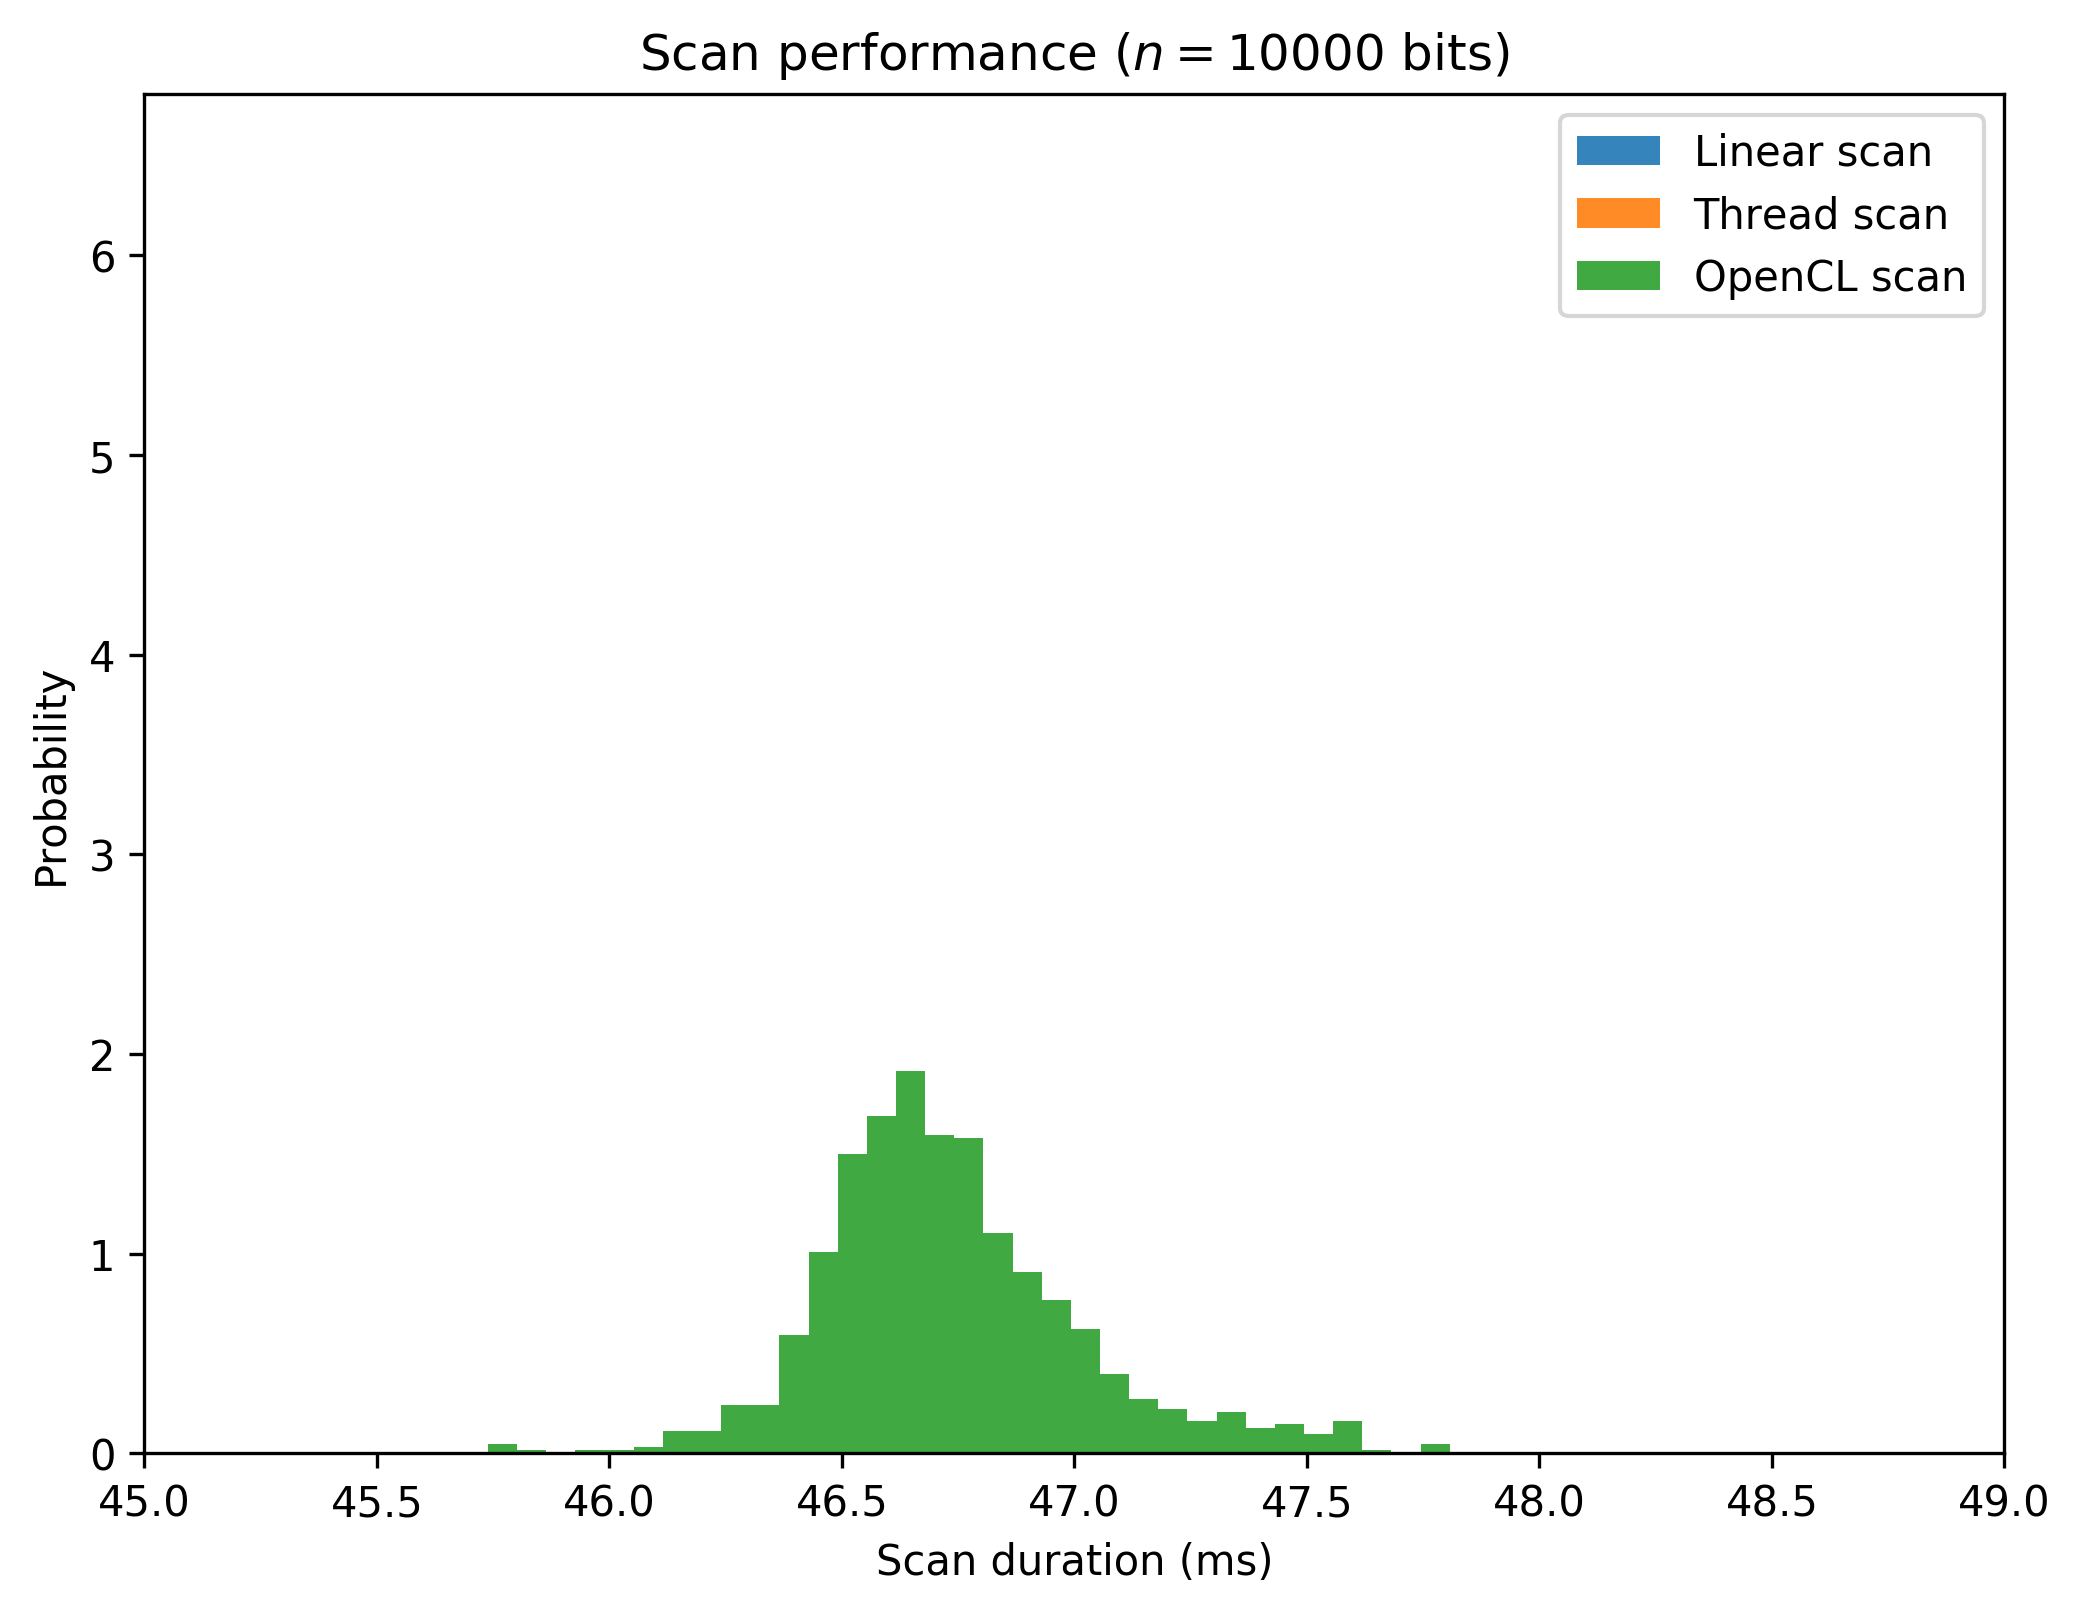
\includegraphics[width=0.7\textwidth]{images02/performance/ec2-p2-scan-10k.png}}

\caption{Scanner comparisons for Amazon EC2 p2.xlarge with Intel Xeon E5-2686v4 processor, 61GB DDR3 RAM, and NVIDIA K80 GPU.
\label{fig:perf-ec2-p2-scanners}}
\end{figure}


\begin{figure}[!htb]
\centering
\subfloat[$n=1,000$, $r=451$, and $H=1,000,000$]{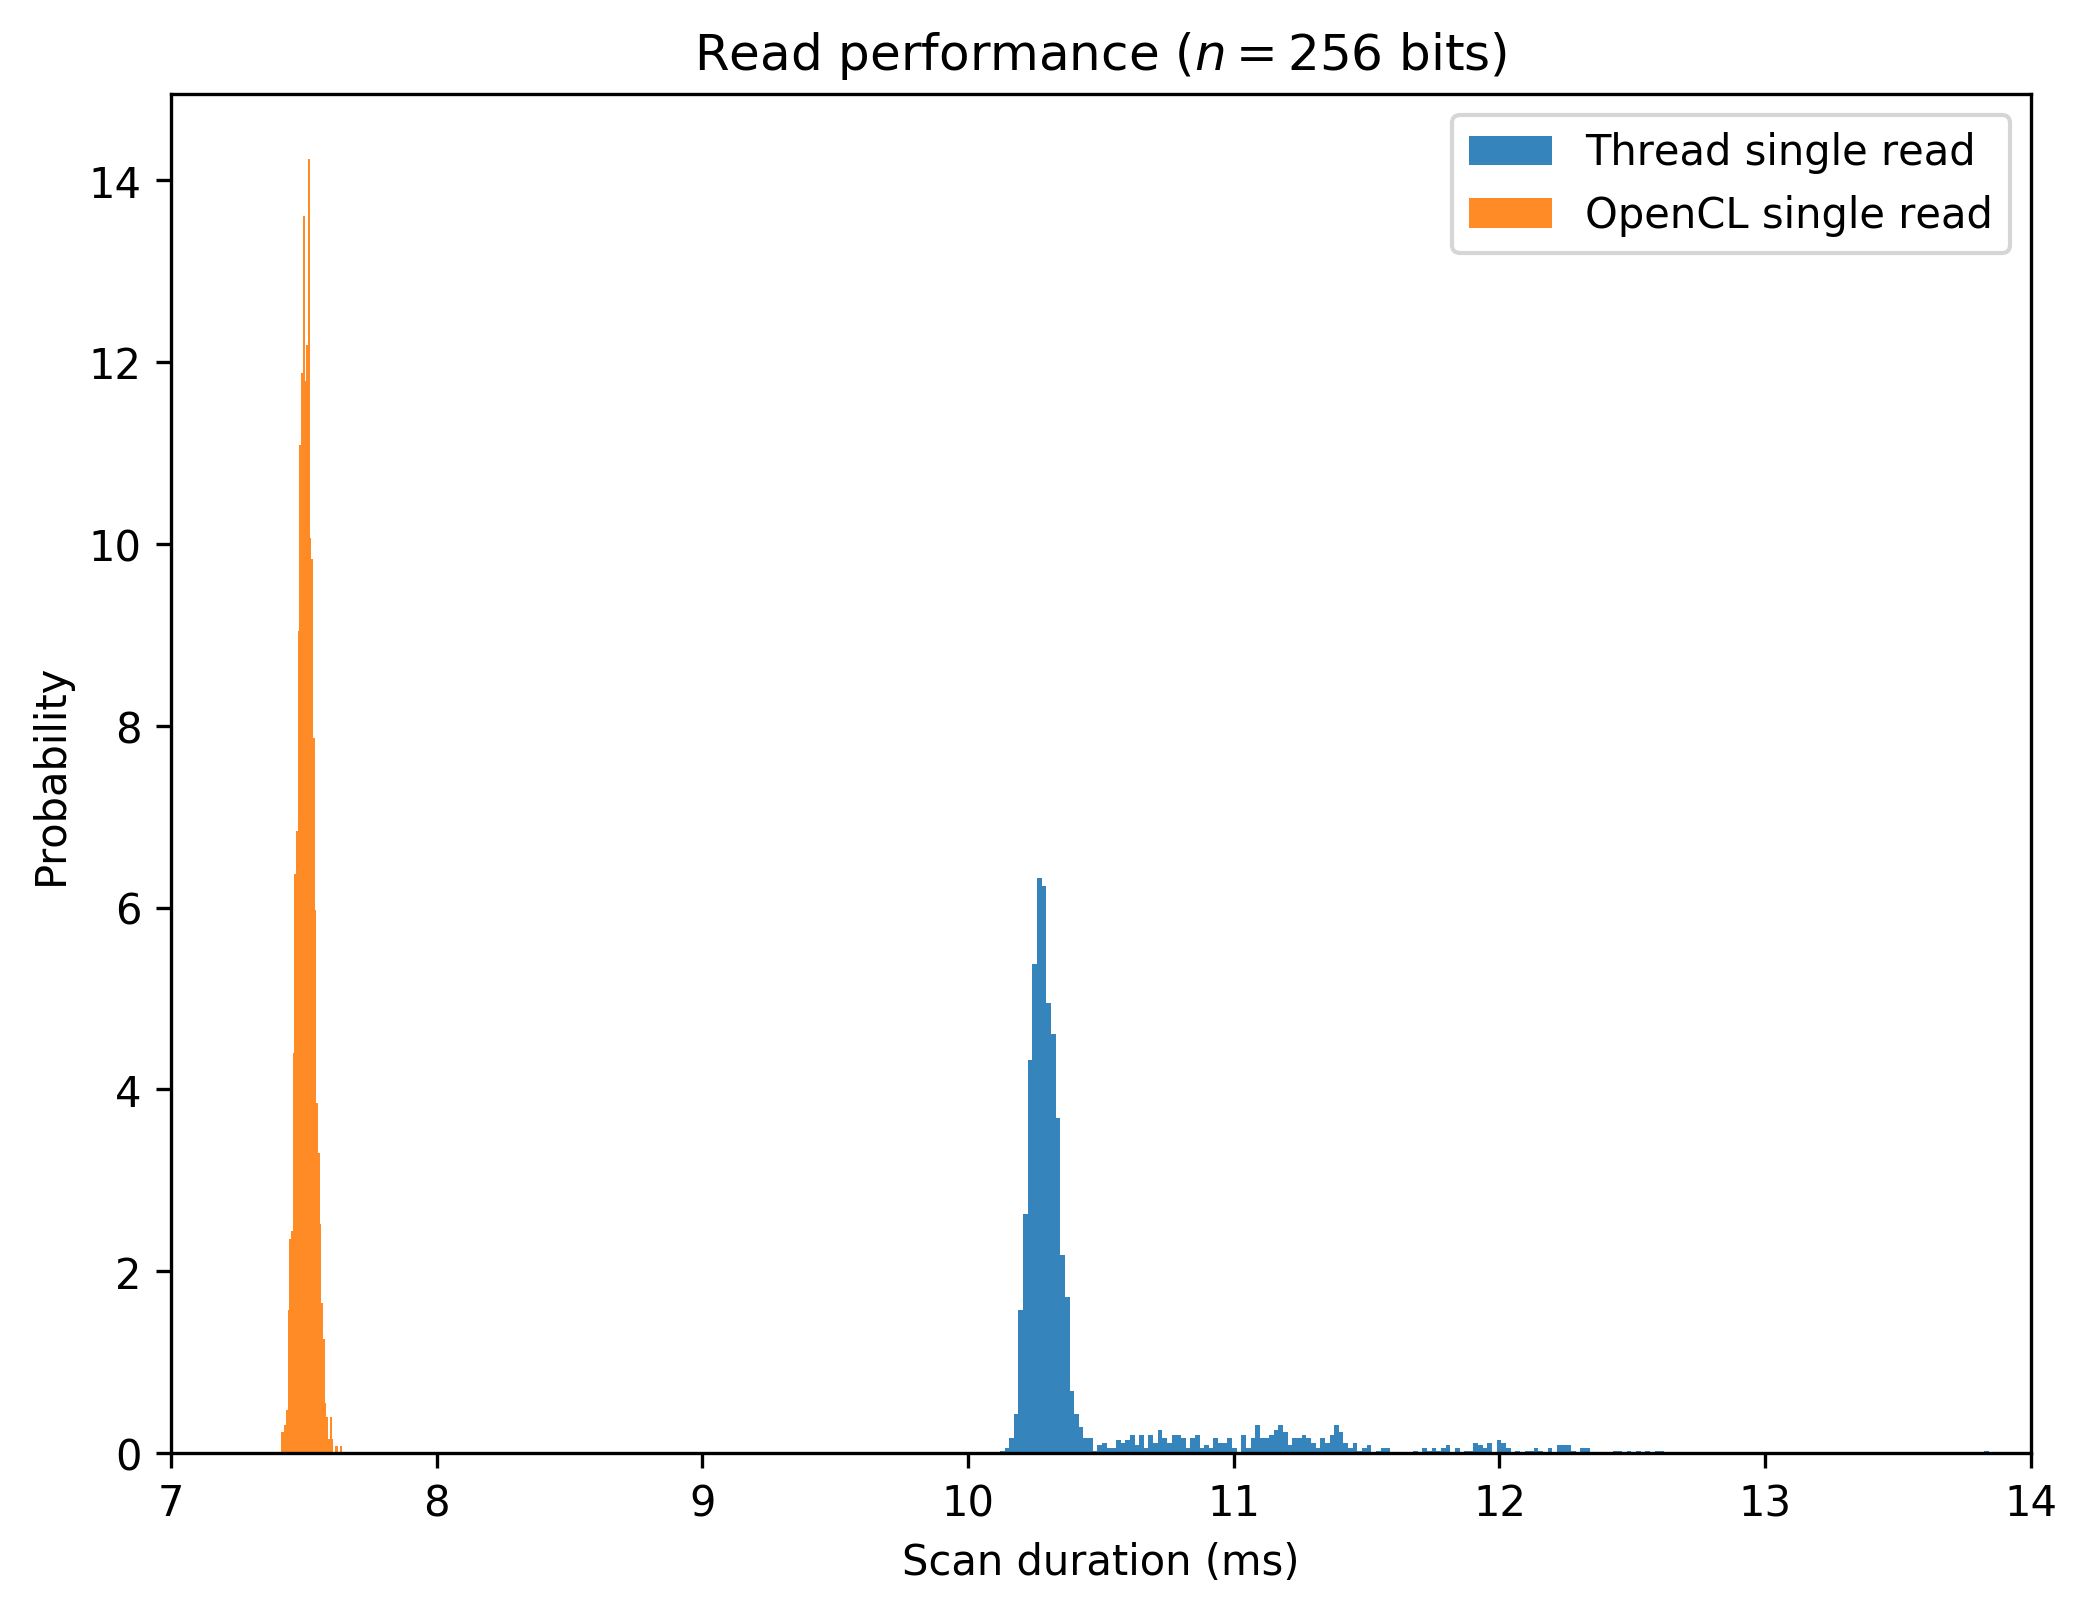
\includegraphics[width=0.7\textwidth]{images02/performance/ec2-p2-read-256.png}}

\subfloat[$n=1,000$, $r=451$, and $H=1,000,000$]{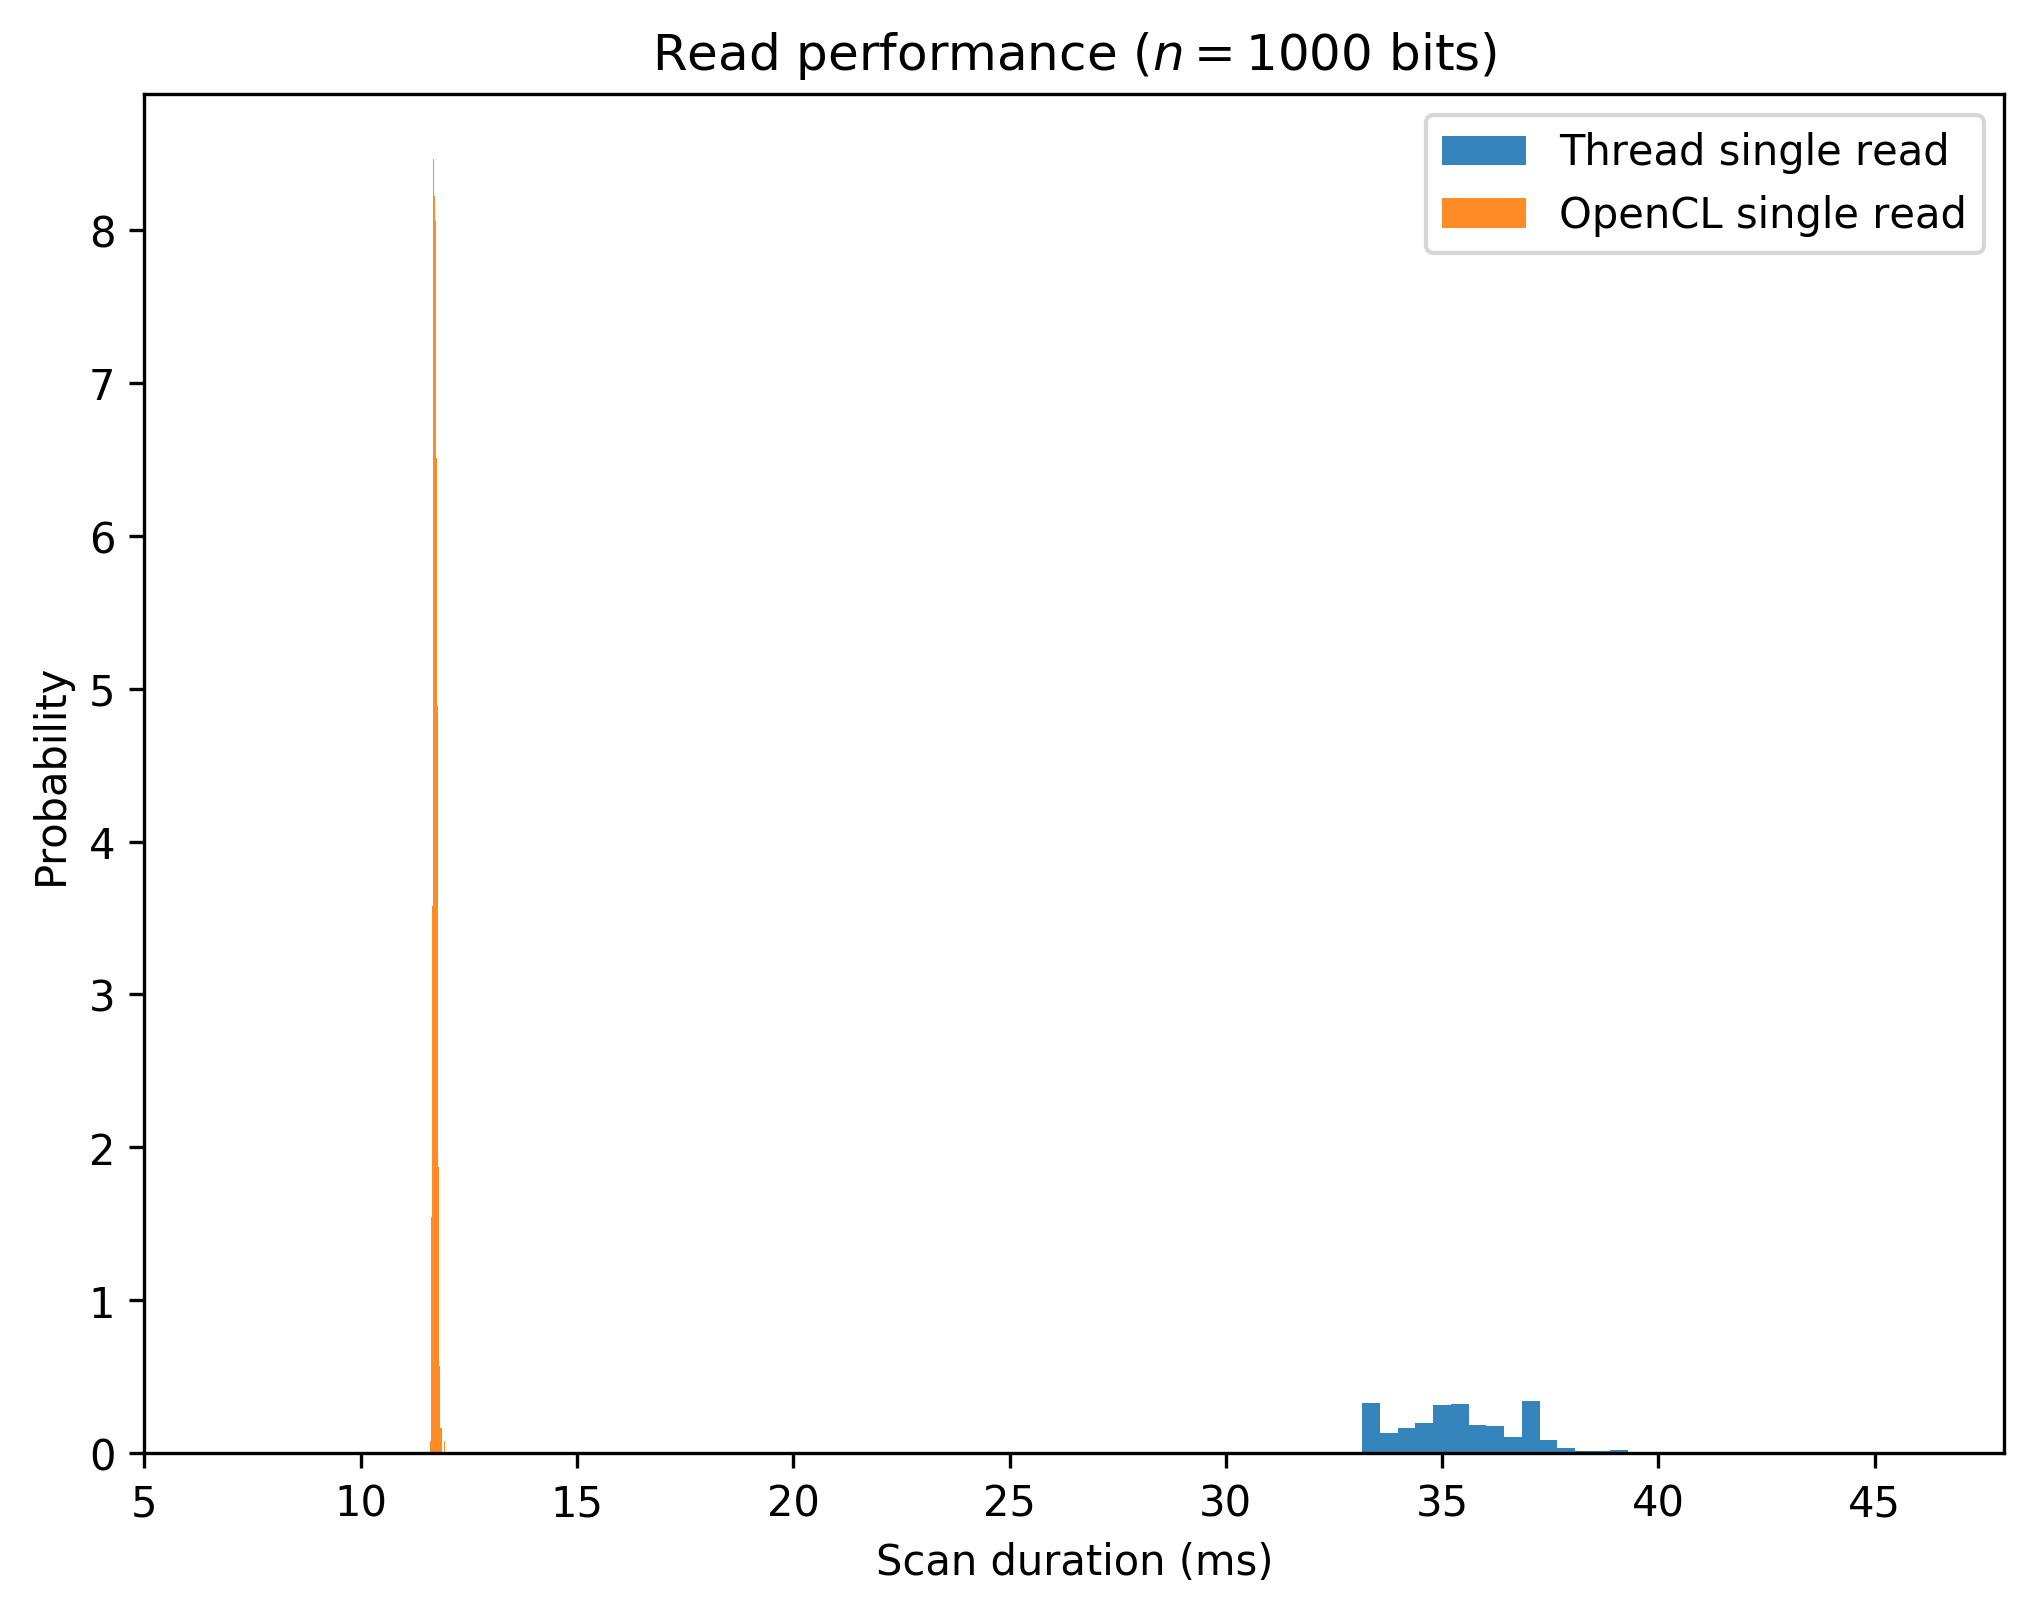
\includegraphics[width=0.7\textwidth]{images02/performance/ec2-p2-read-1000.png}}

\subfloat[$n=10,000$, $r=4805$, and $H=1,000,000$]{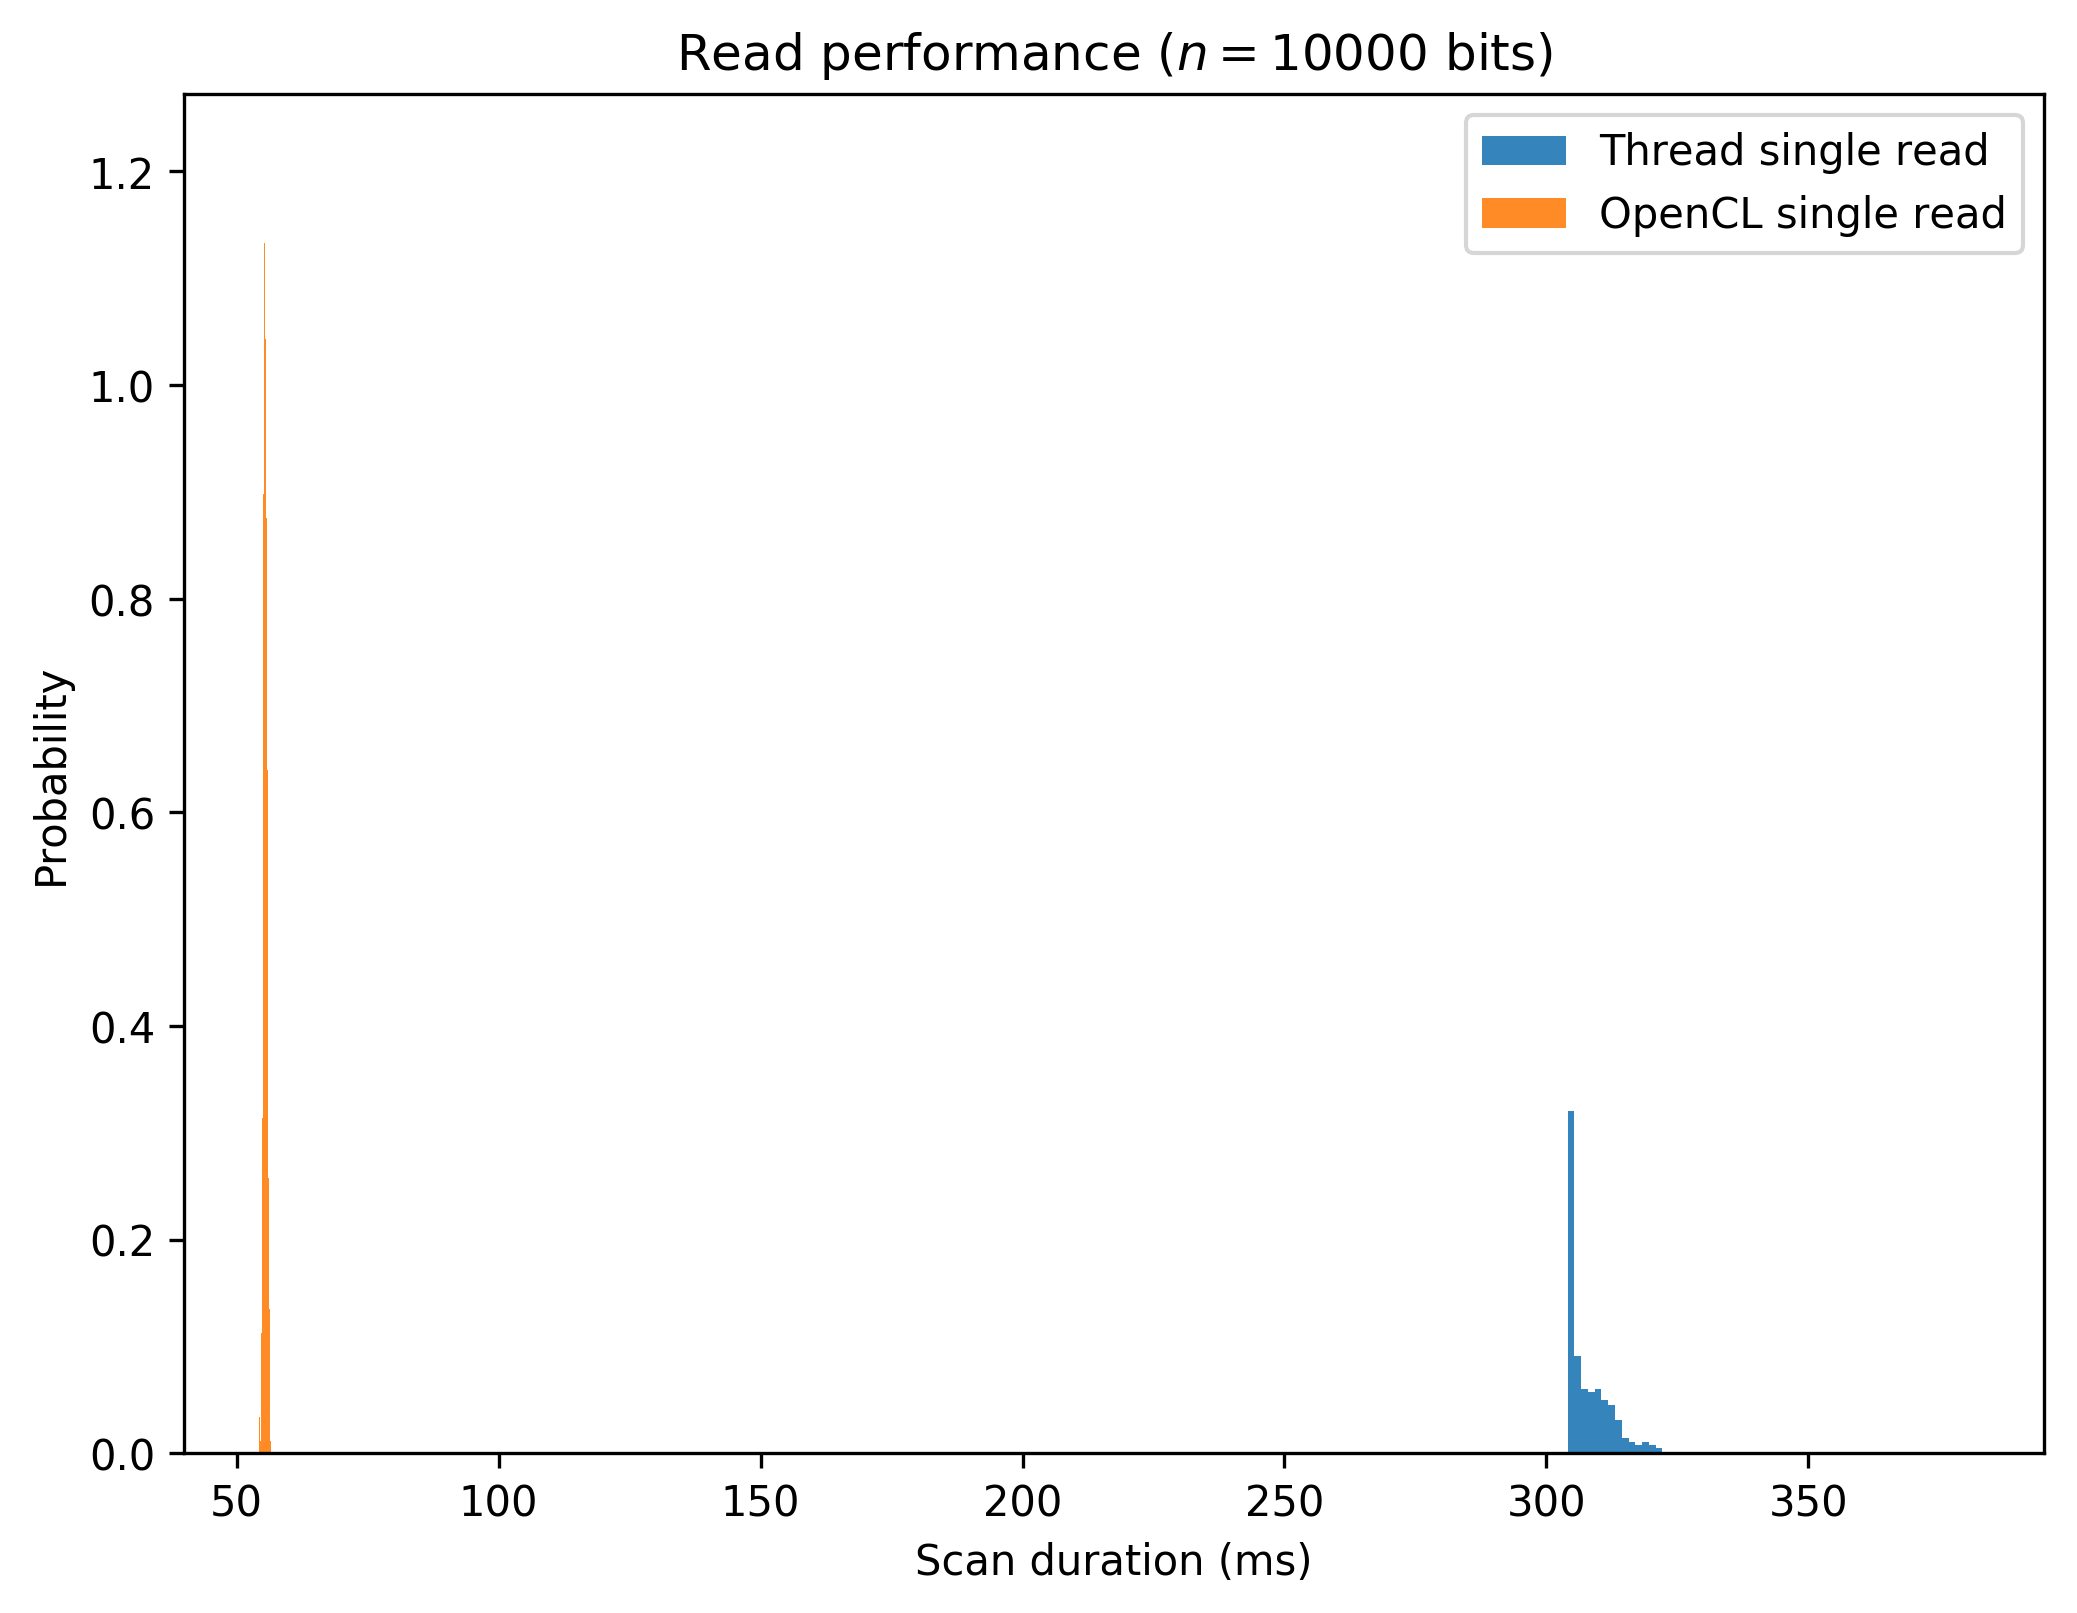
\includegraphics[width=0.7\textwidth]{images02/performance/ec2-p2-read-10k.png}}

\caption{Read operation comparisons for Amazon EC2 p2.xlarge with Intel Xeon E5-2686v4 processor, 61GB DDR3 RAM, and NVIDIA K80 GPU.
\label{fig:perf-ec2-p2-read}}
\end{figure}

\begin{figure}[!htb]
\centering
\subfloat[$n=1,000$, $r=451$, and $H=1,000,000$]{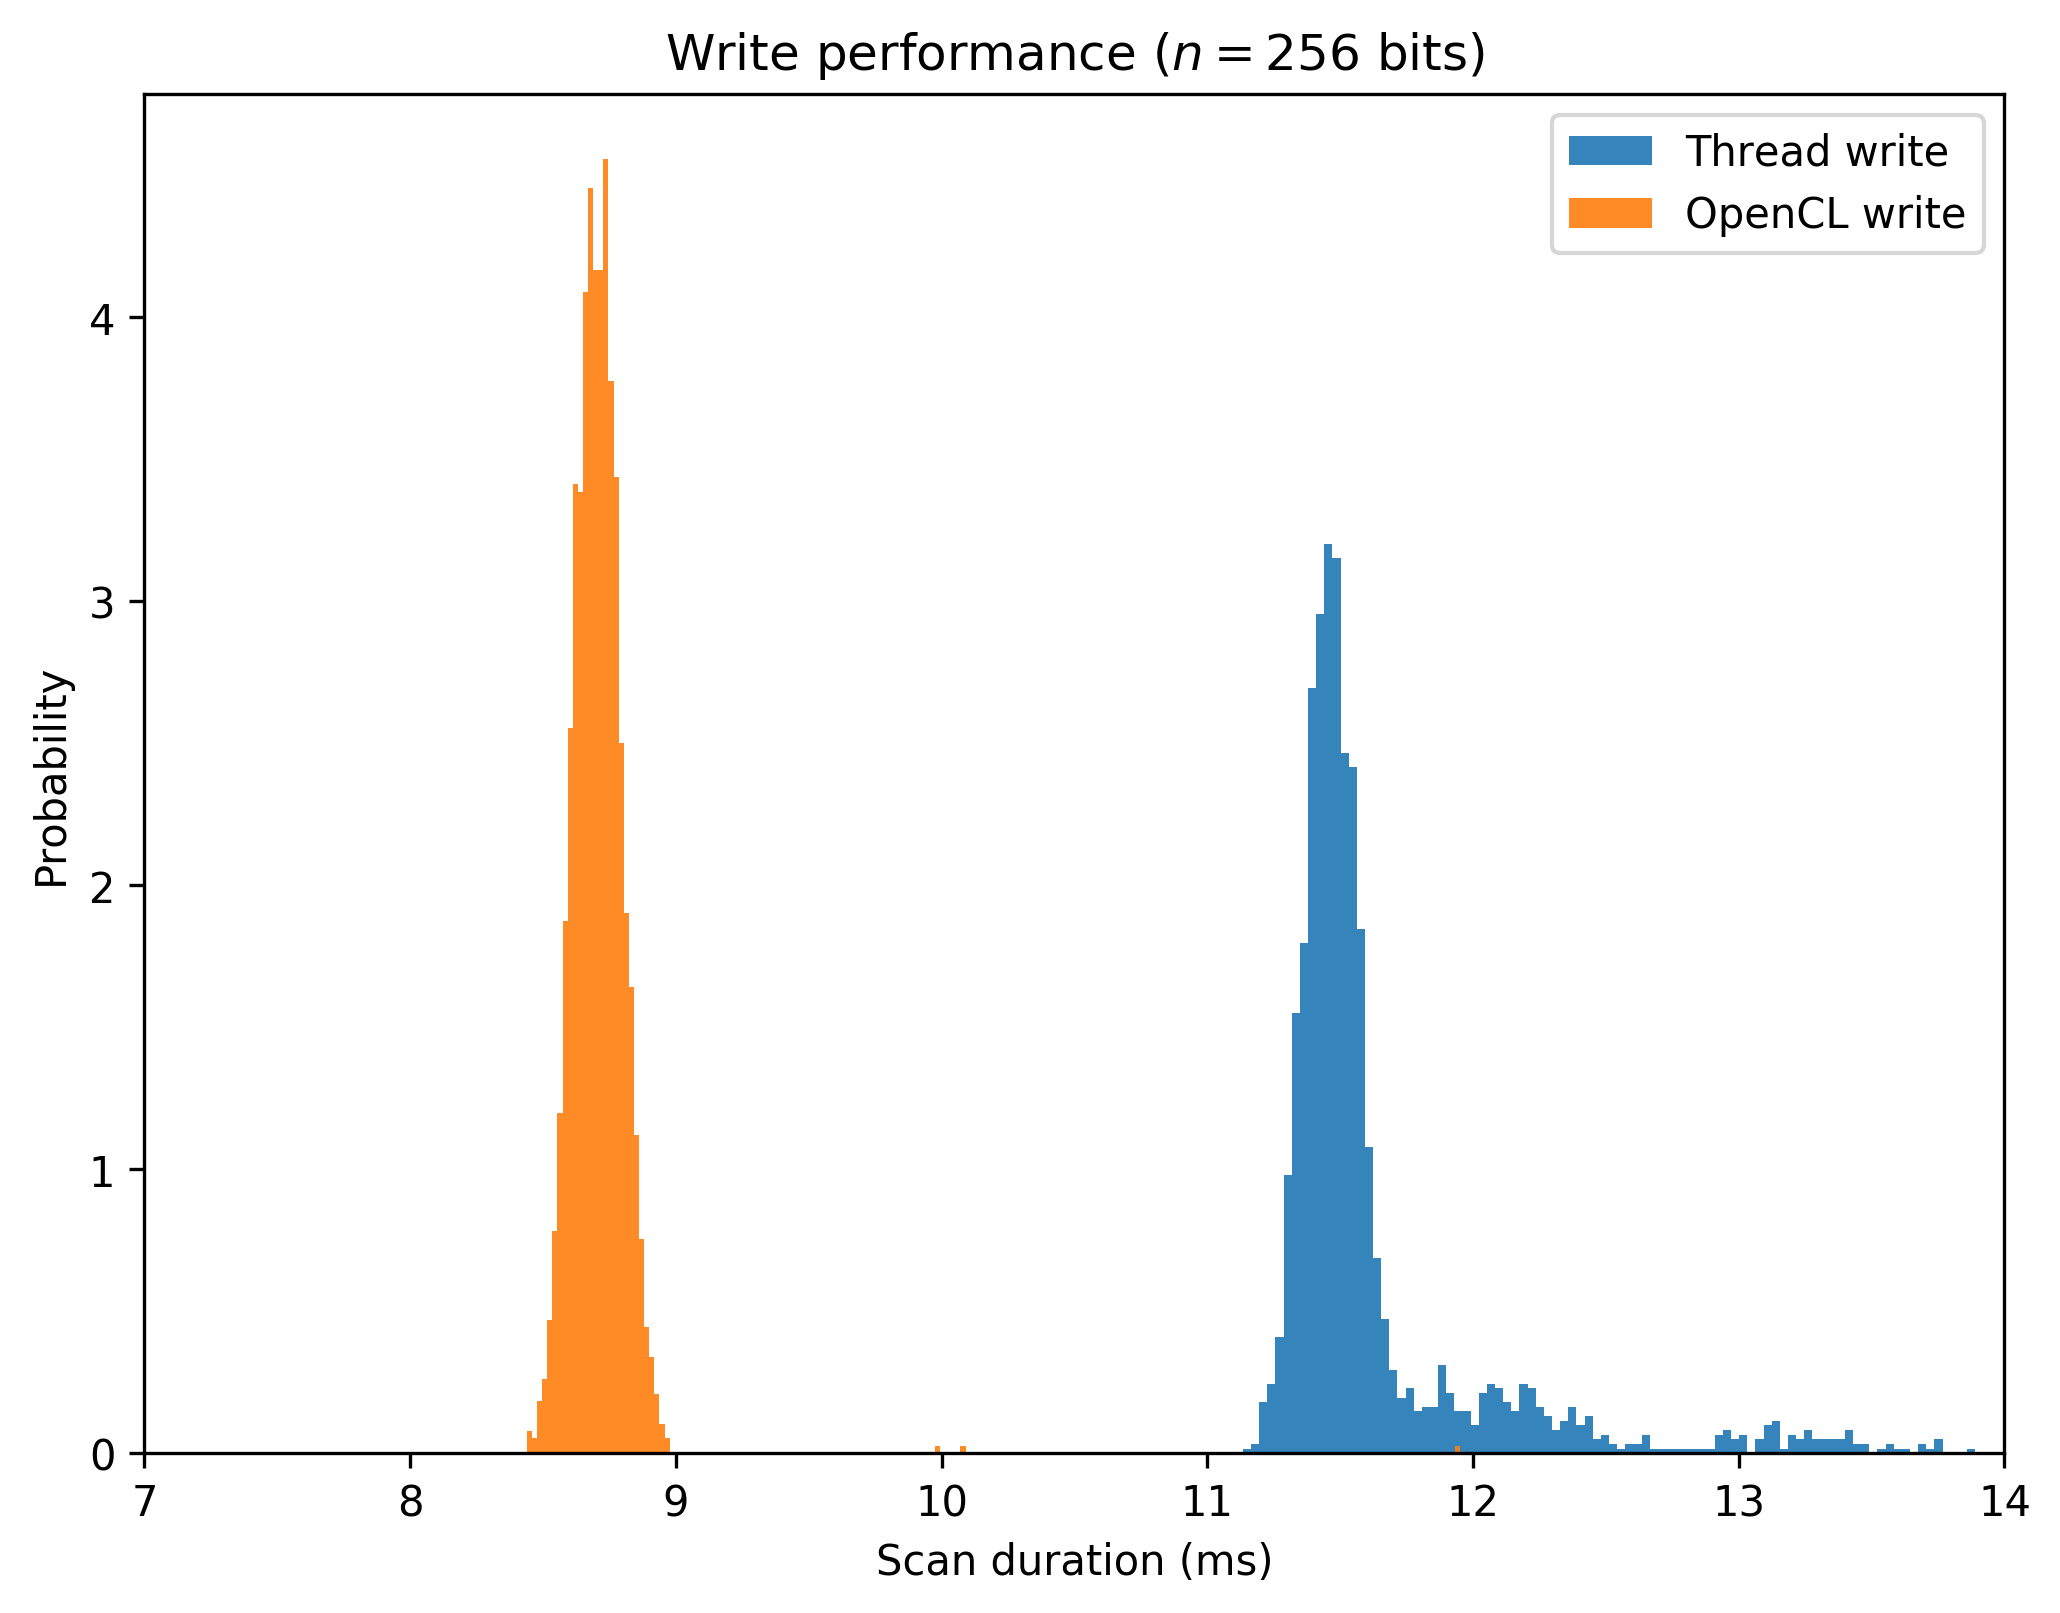
\includegraphics[width=0.7\textwidth]{images02/performance/ec2-p2-write-256.png}}

\subfloat[$n=1,000$, $r=451$, and $H=1,000,000$]{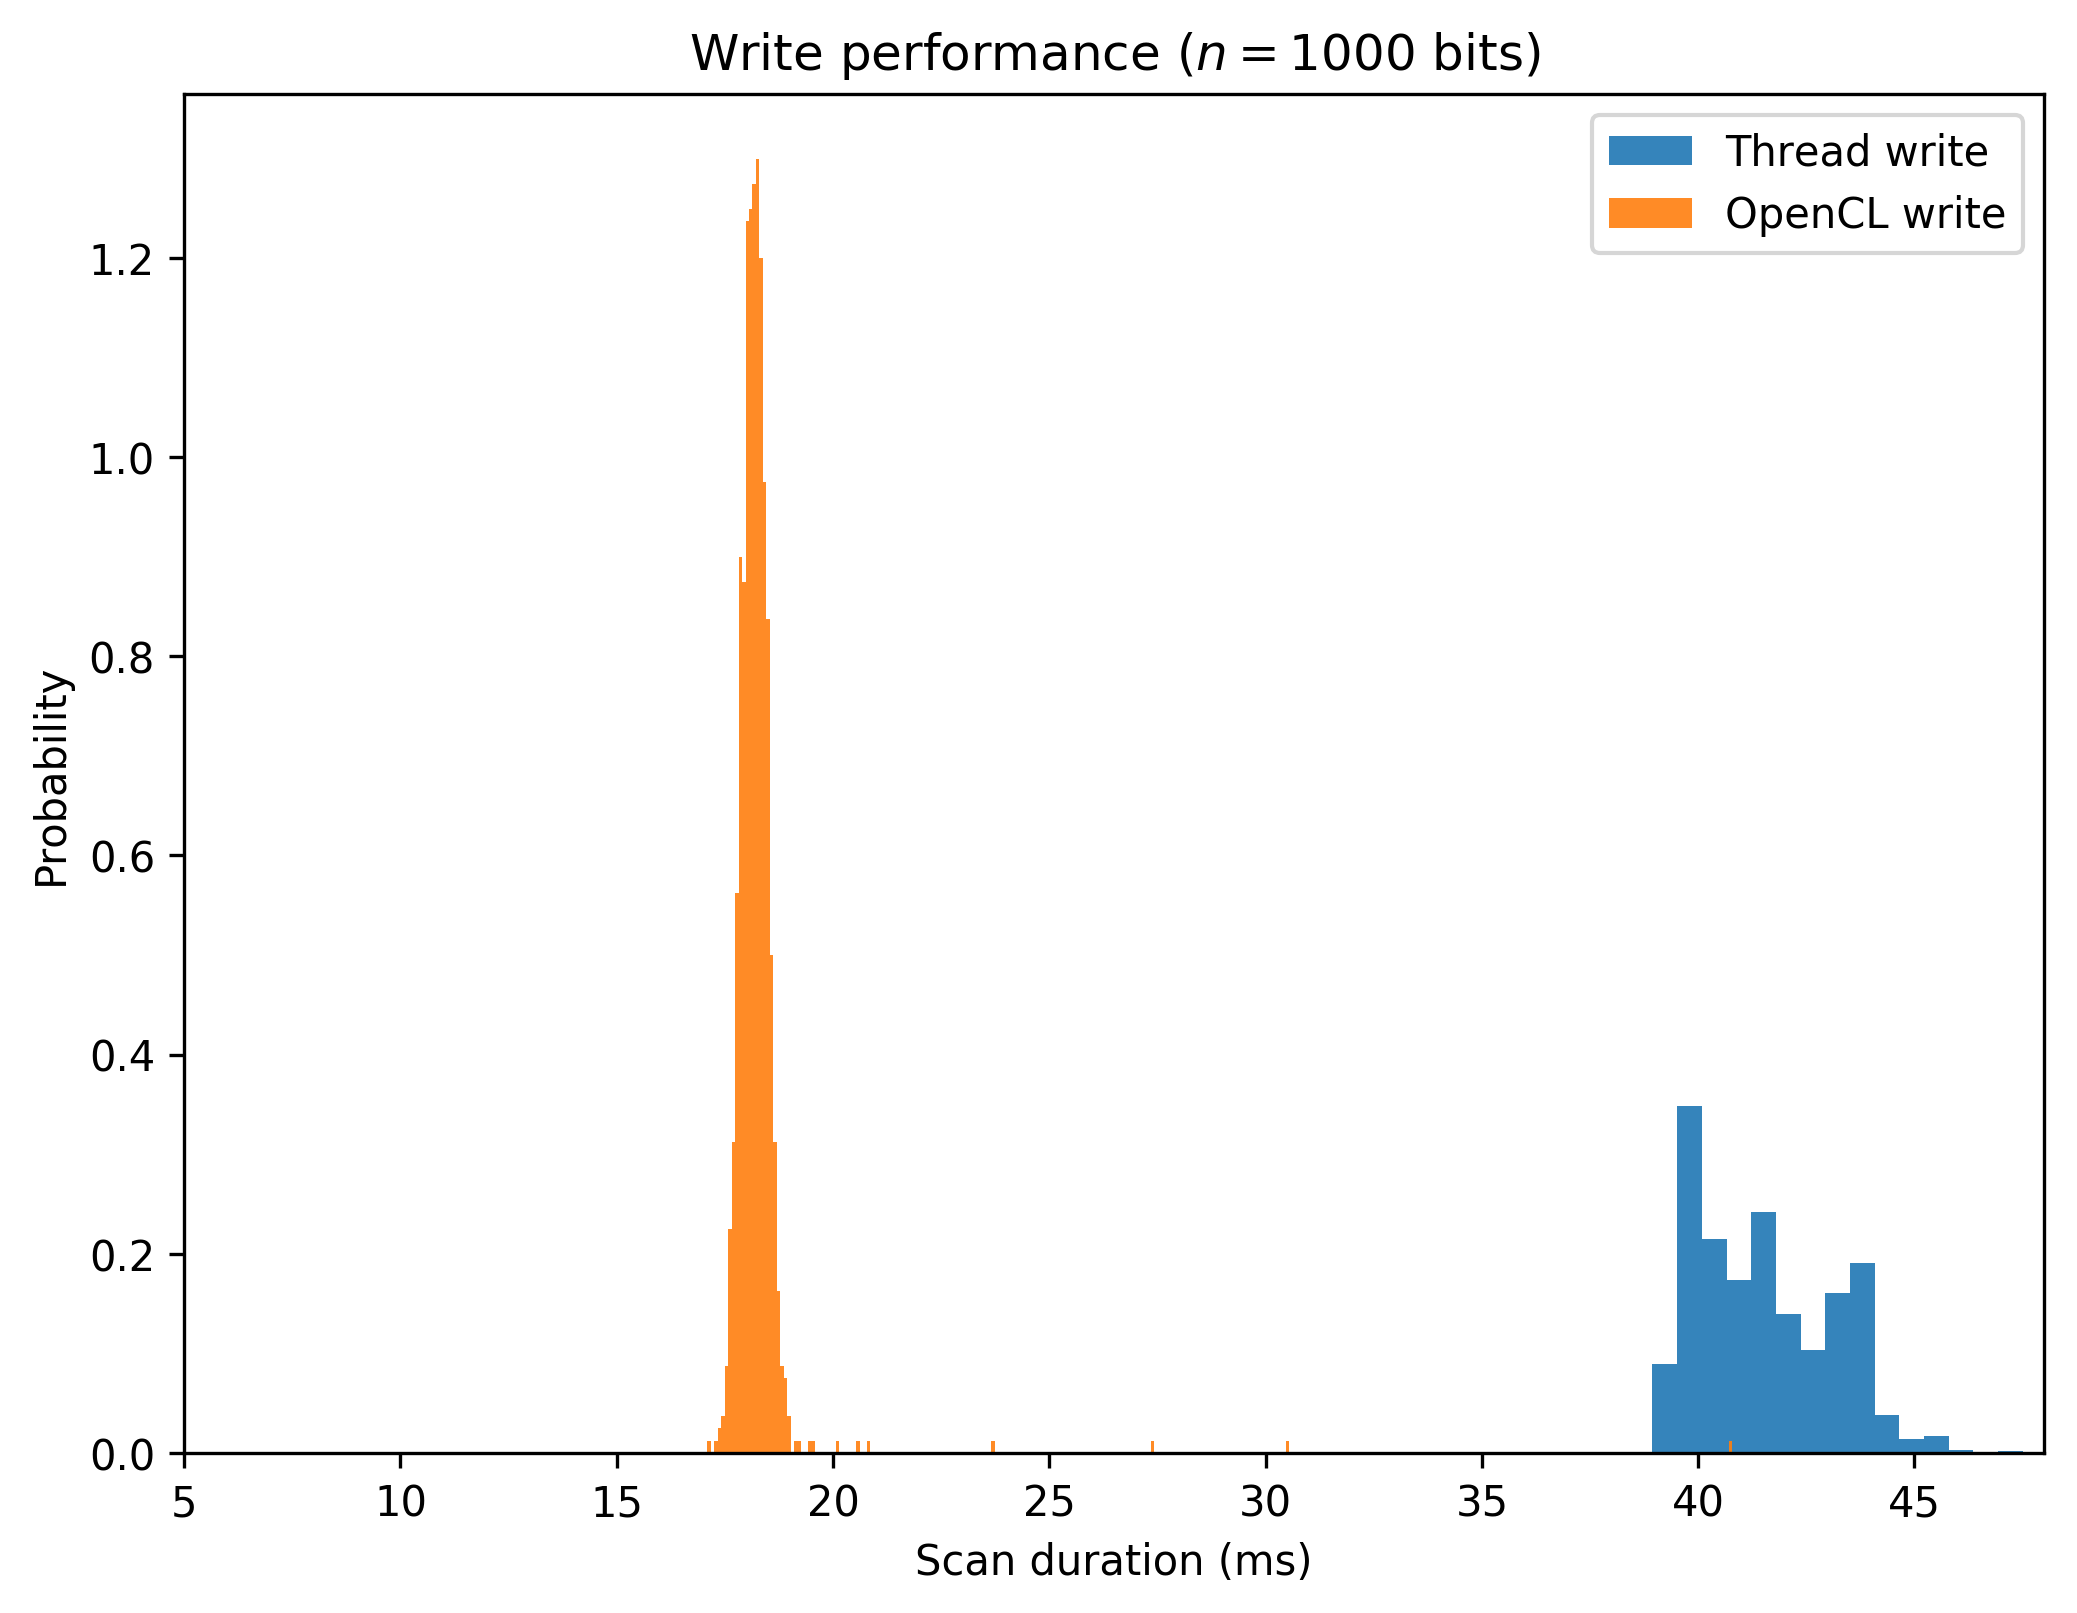
\includegraphics[width=0.7\textwidth]{images02/performance/ec2-p2-write-1000.png}}

\subfloat[$n=10,000$, $r=4805$, and $H=1,000,000$]{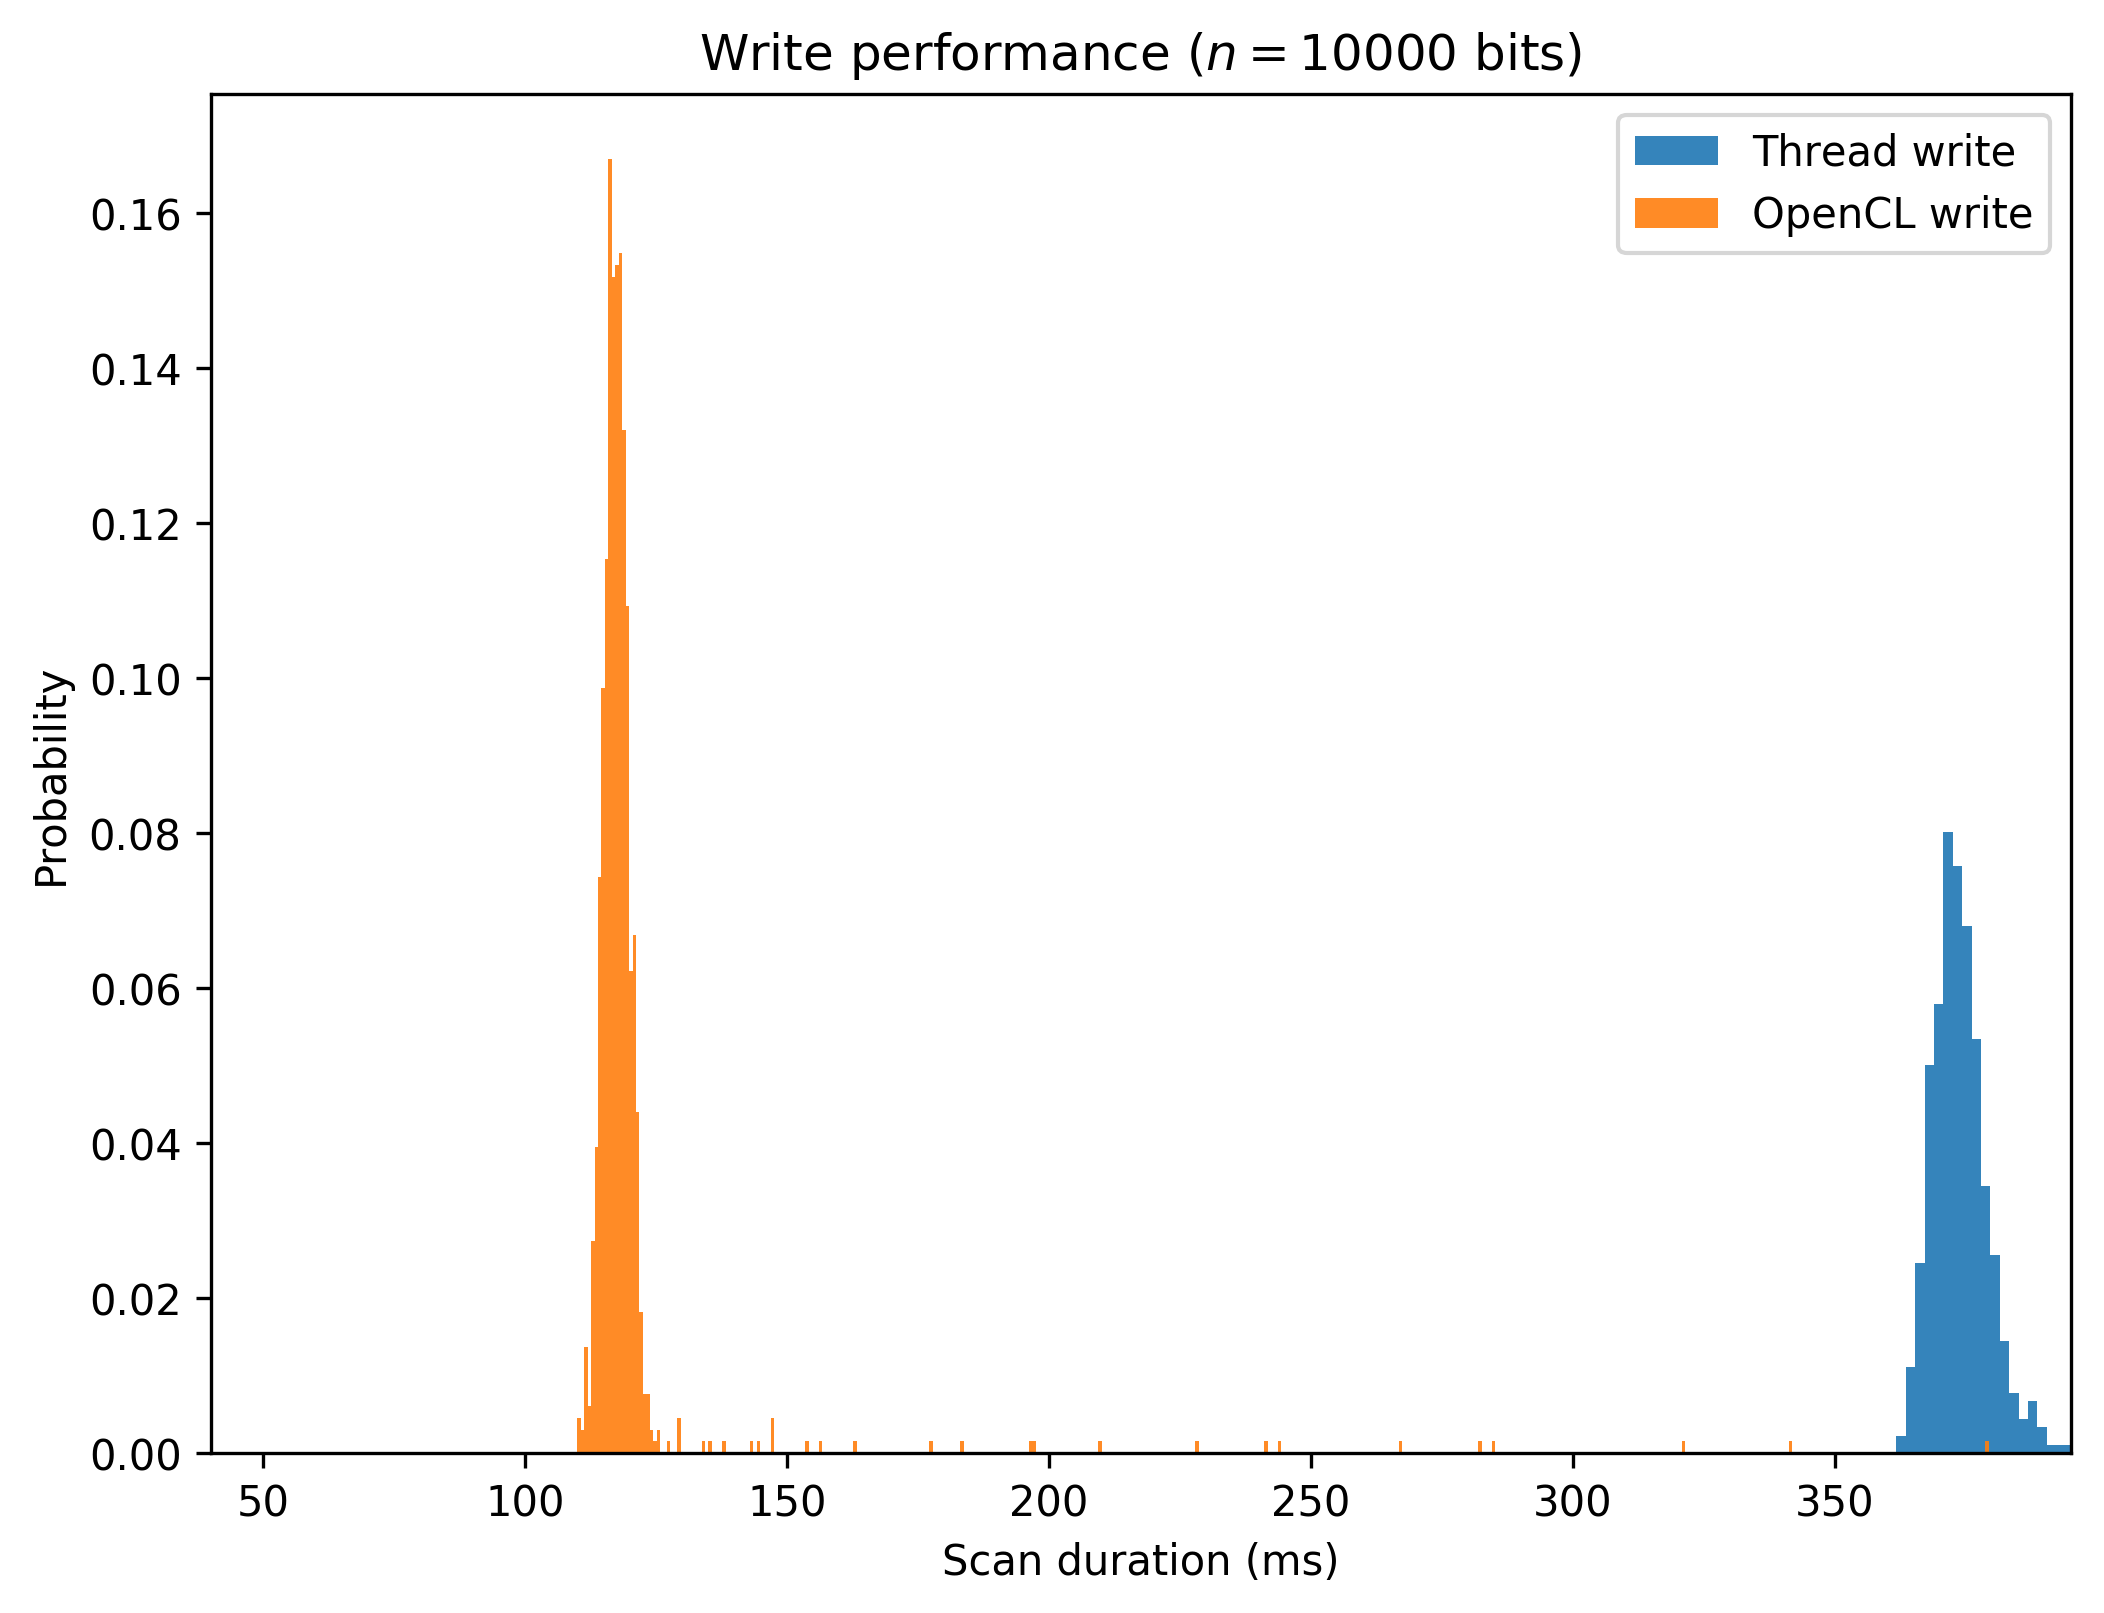
\includegraphics[width=0.7\textwidth]{images02/performance/ec2-p2-write-10k.png}}

\caption{Write operation comparisons for Amazon EC2 p2.xlarge with Intel Xeon E5-2686v4 processor, 61GB DDR3 RAM, and NVIDIA K80 GPU.
\label{fig:perf-ec2-p2-write}}
\end{figure}




% -------------------------
% -------------------------
% -------------------------




\begin{table}[!htb]
\centering
\begin{tabular}{lrrr}
    \toprule
    & \textbf{256 bits} & \textbf{1,000 bits} & \textbf{10,000 bits} \\ \hline
	\hline
	Kernel & Duration (ms) & Duration (ms) & Duration (ms) \\ \hline
    \hline
    single\_scan0 & 0.36 & 0.69 & 20.60 \\
    single\_scan1 & 0.36 & 0.54 &  4.94 \\
    single\_scan2 & 0.73 & 0.85 &  5.01 \\
    single\_scan3 & 0.63 & 1.02 &  6.07 \\
    single\_scan4 & 1.05 & 1.10 &  5.99 \\
    single\_scan5 & 0.62 & 0.95 &  5.36 \\
	single\_scan5\_unroll & & & \\
    single\_scan6 & 1.01 & 1.04 &  5.96 \\ \hline
    \hline
	Scanner & Duration (ms) & Duration (ms) & Duration (ms) \\ \hline
    Linear scan & 17.60 & 58.34 & 540.97 \\
    Thread scan &  5.19 & 16.39 & 198.74 \\
    OpenCL scan &  0.63 &  0.85 &   5.74 \\ \hline
    \hline
	Operation & Duration (ms) & Duration (ms) & Duration (ms) \\ \hline
    Thread write       & 7.59 & 28.47 & 222.08 \\
    Thread single read & 6.17 & 17.44 & 145.01 \\
    OpenCL write       & 2.33 &  8.77 &  80.48 \\
    OpenCL single read & 1.01 &  1.82 &  13.99 \\
    \hline
\end{tabular}
\caption{Amazon EC2 p3.2xlarge with Intel Xeon E5-2686v4 processor, 488GB DDR3 RAM, and NVIDIA Tesla V100 GPU. The SDM settings were: (i) $n=256$, $r=103$, and $H=1,000,000$; (ii) $n=1,000$, $r=451$, and $H=1,000,000$; and (iii) $n=10,000$, $r=4850$, and $H=1,000,000$. There is no benchmark for kernel single\_scan5\_unroll because it returns the wrong result in this GPU. The problem is related with the premises of the optimization used by this kernel, which are not true for this GPU.
For the histogram of durations, see Figures \ref{fig:perf-ec2-p3-kernels}, \ref{fig:perf-ec2-p3-scanners}, \ref{fig:perf-ec2-p3-read}, and \ref{fig:perf-ec2-p3-write}.
\label{tab:perf-ec2-p3}}
\end{table}





\begin{figure}[!htb]
\centering
\subfloat[$n=256$, $r=103$, and $H=1,000,000$]{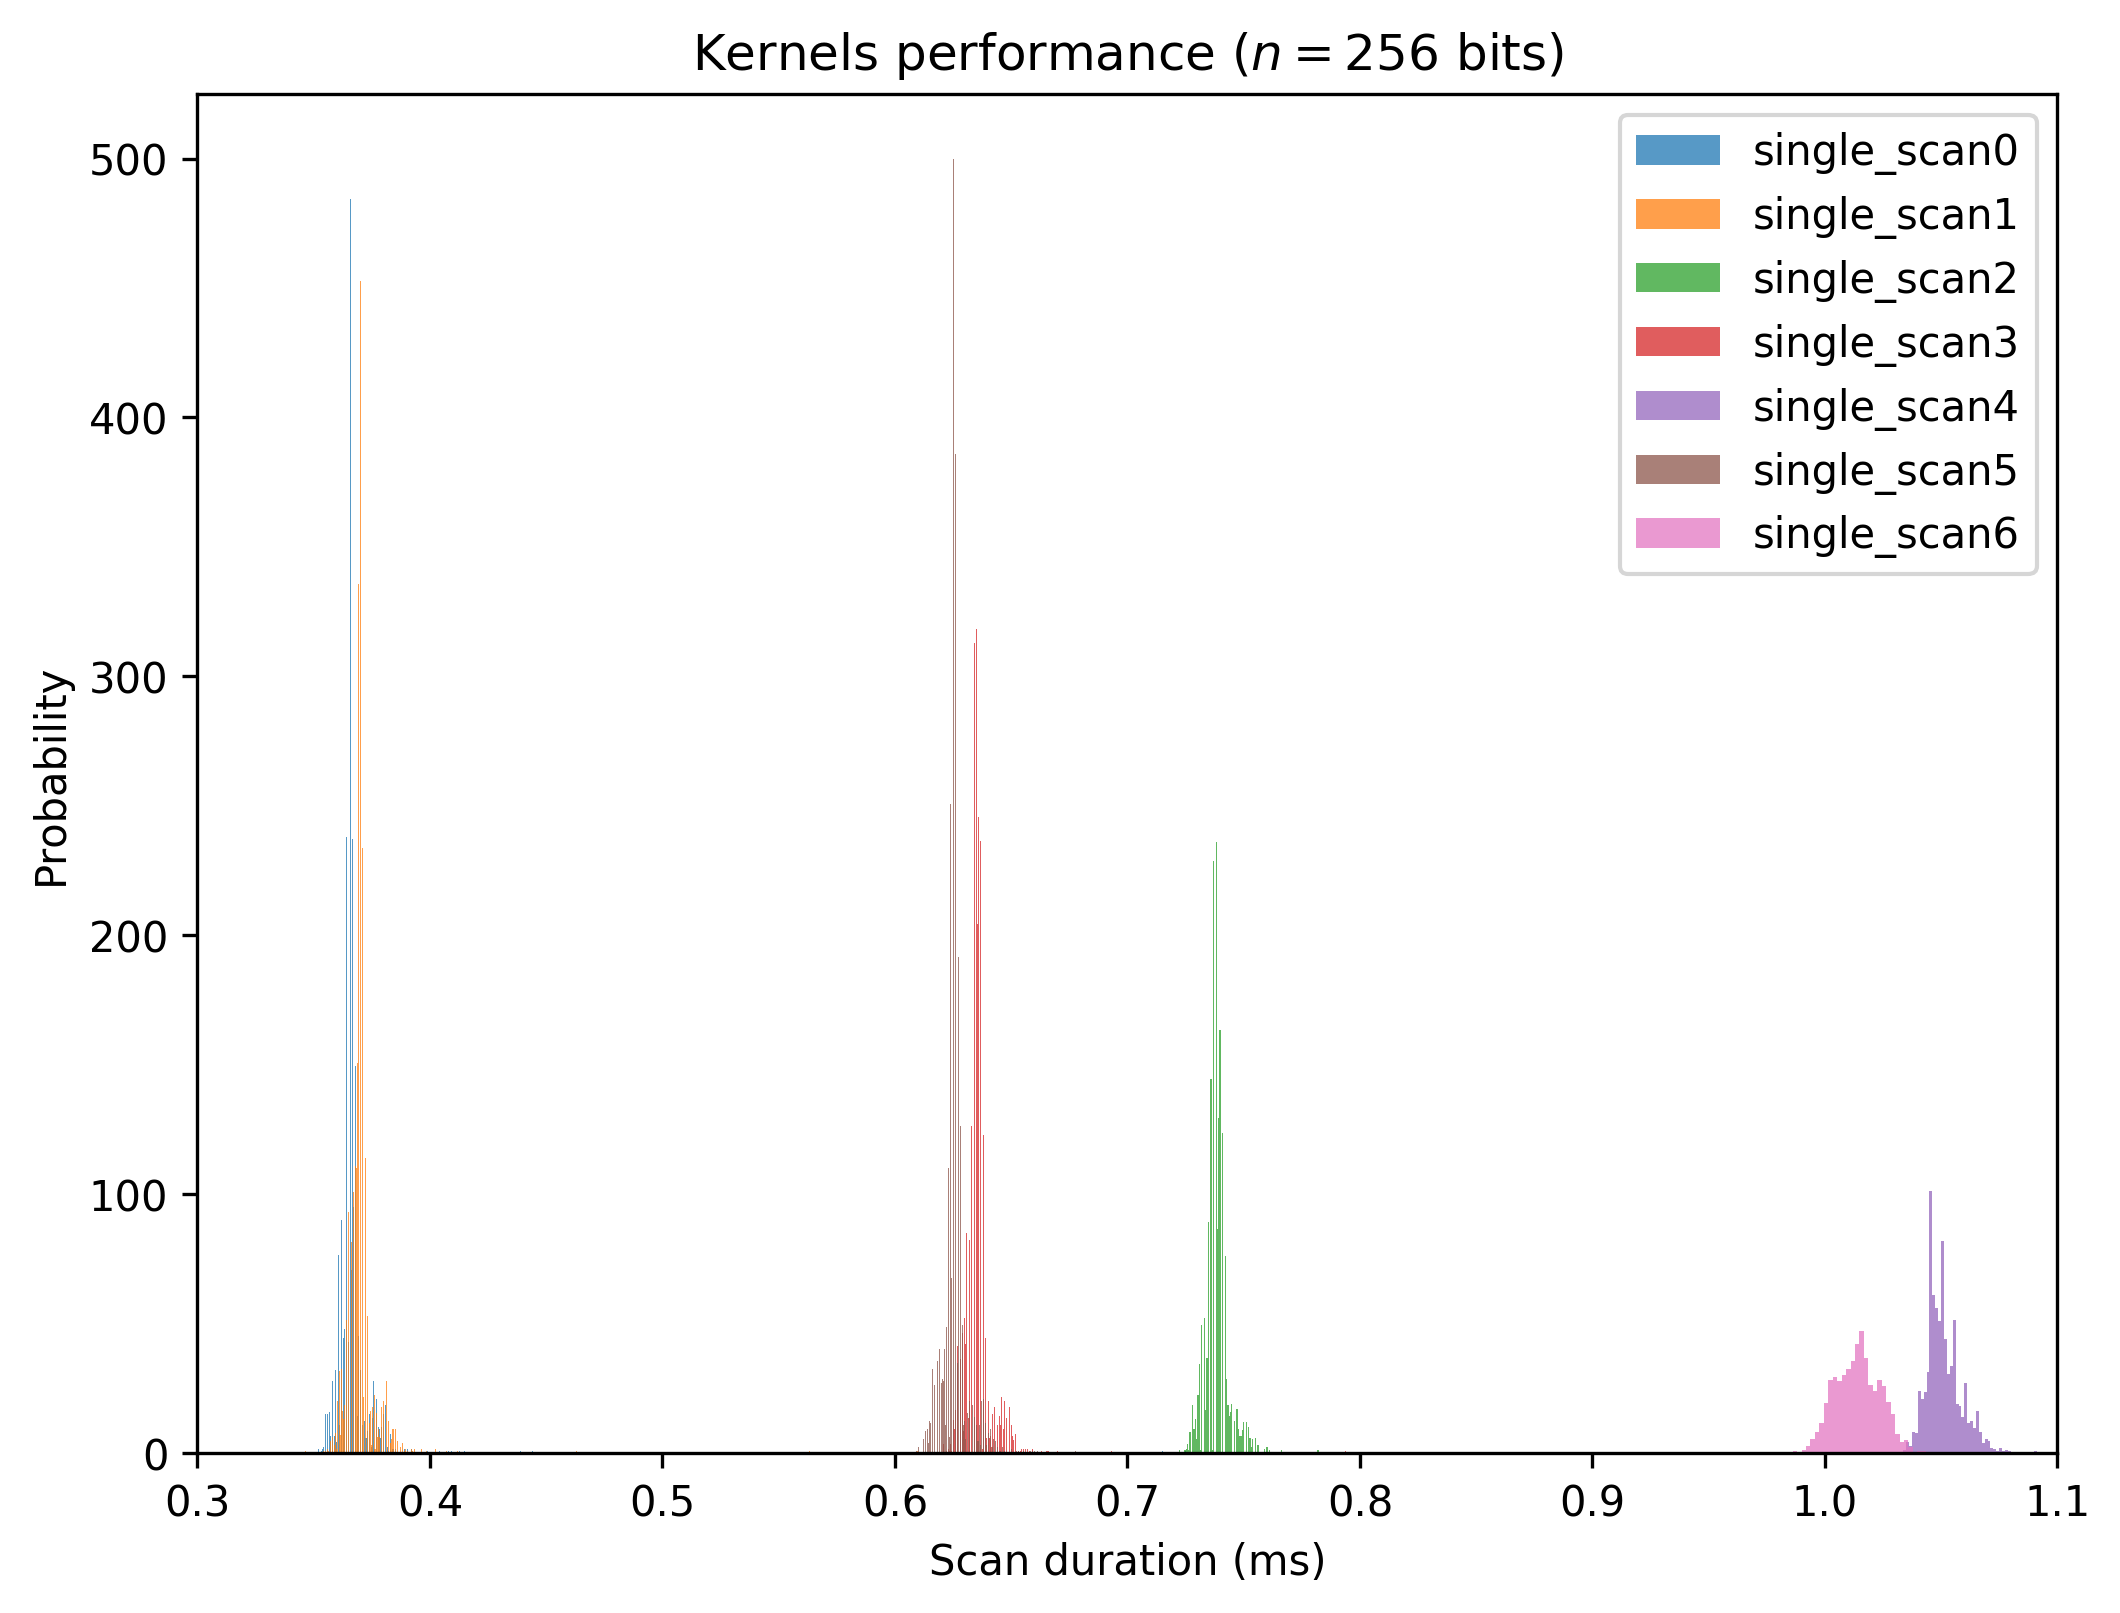
\includegraphics[width=0.7\textwidth]{images02/performance/ec2-p3-kernels-256.png}}

\subfloat[$n=1,000$, $r=451$, and $H=1,000,000$]{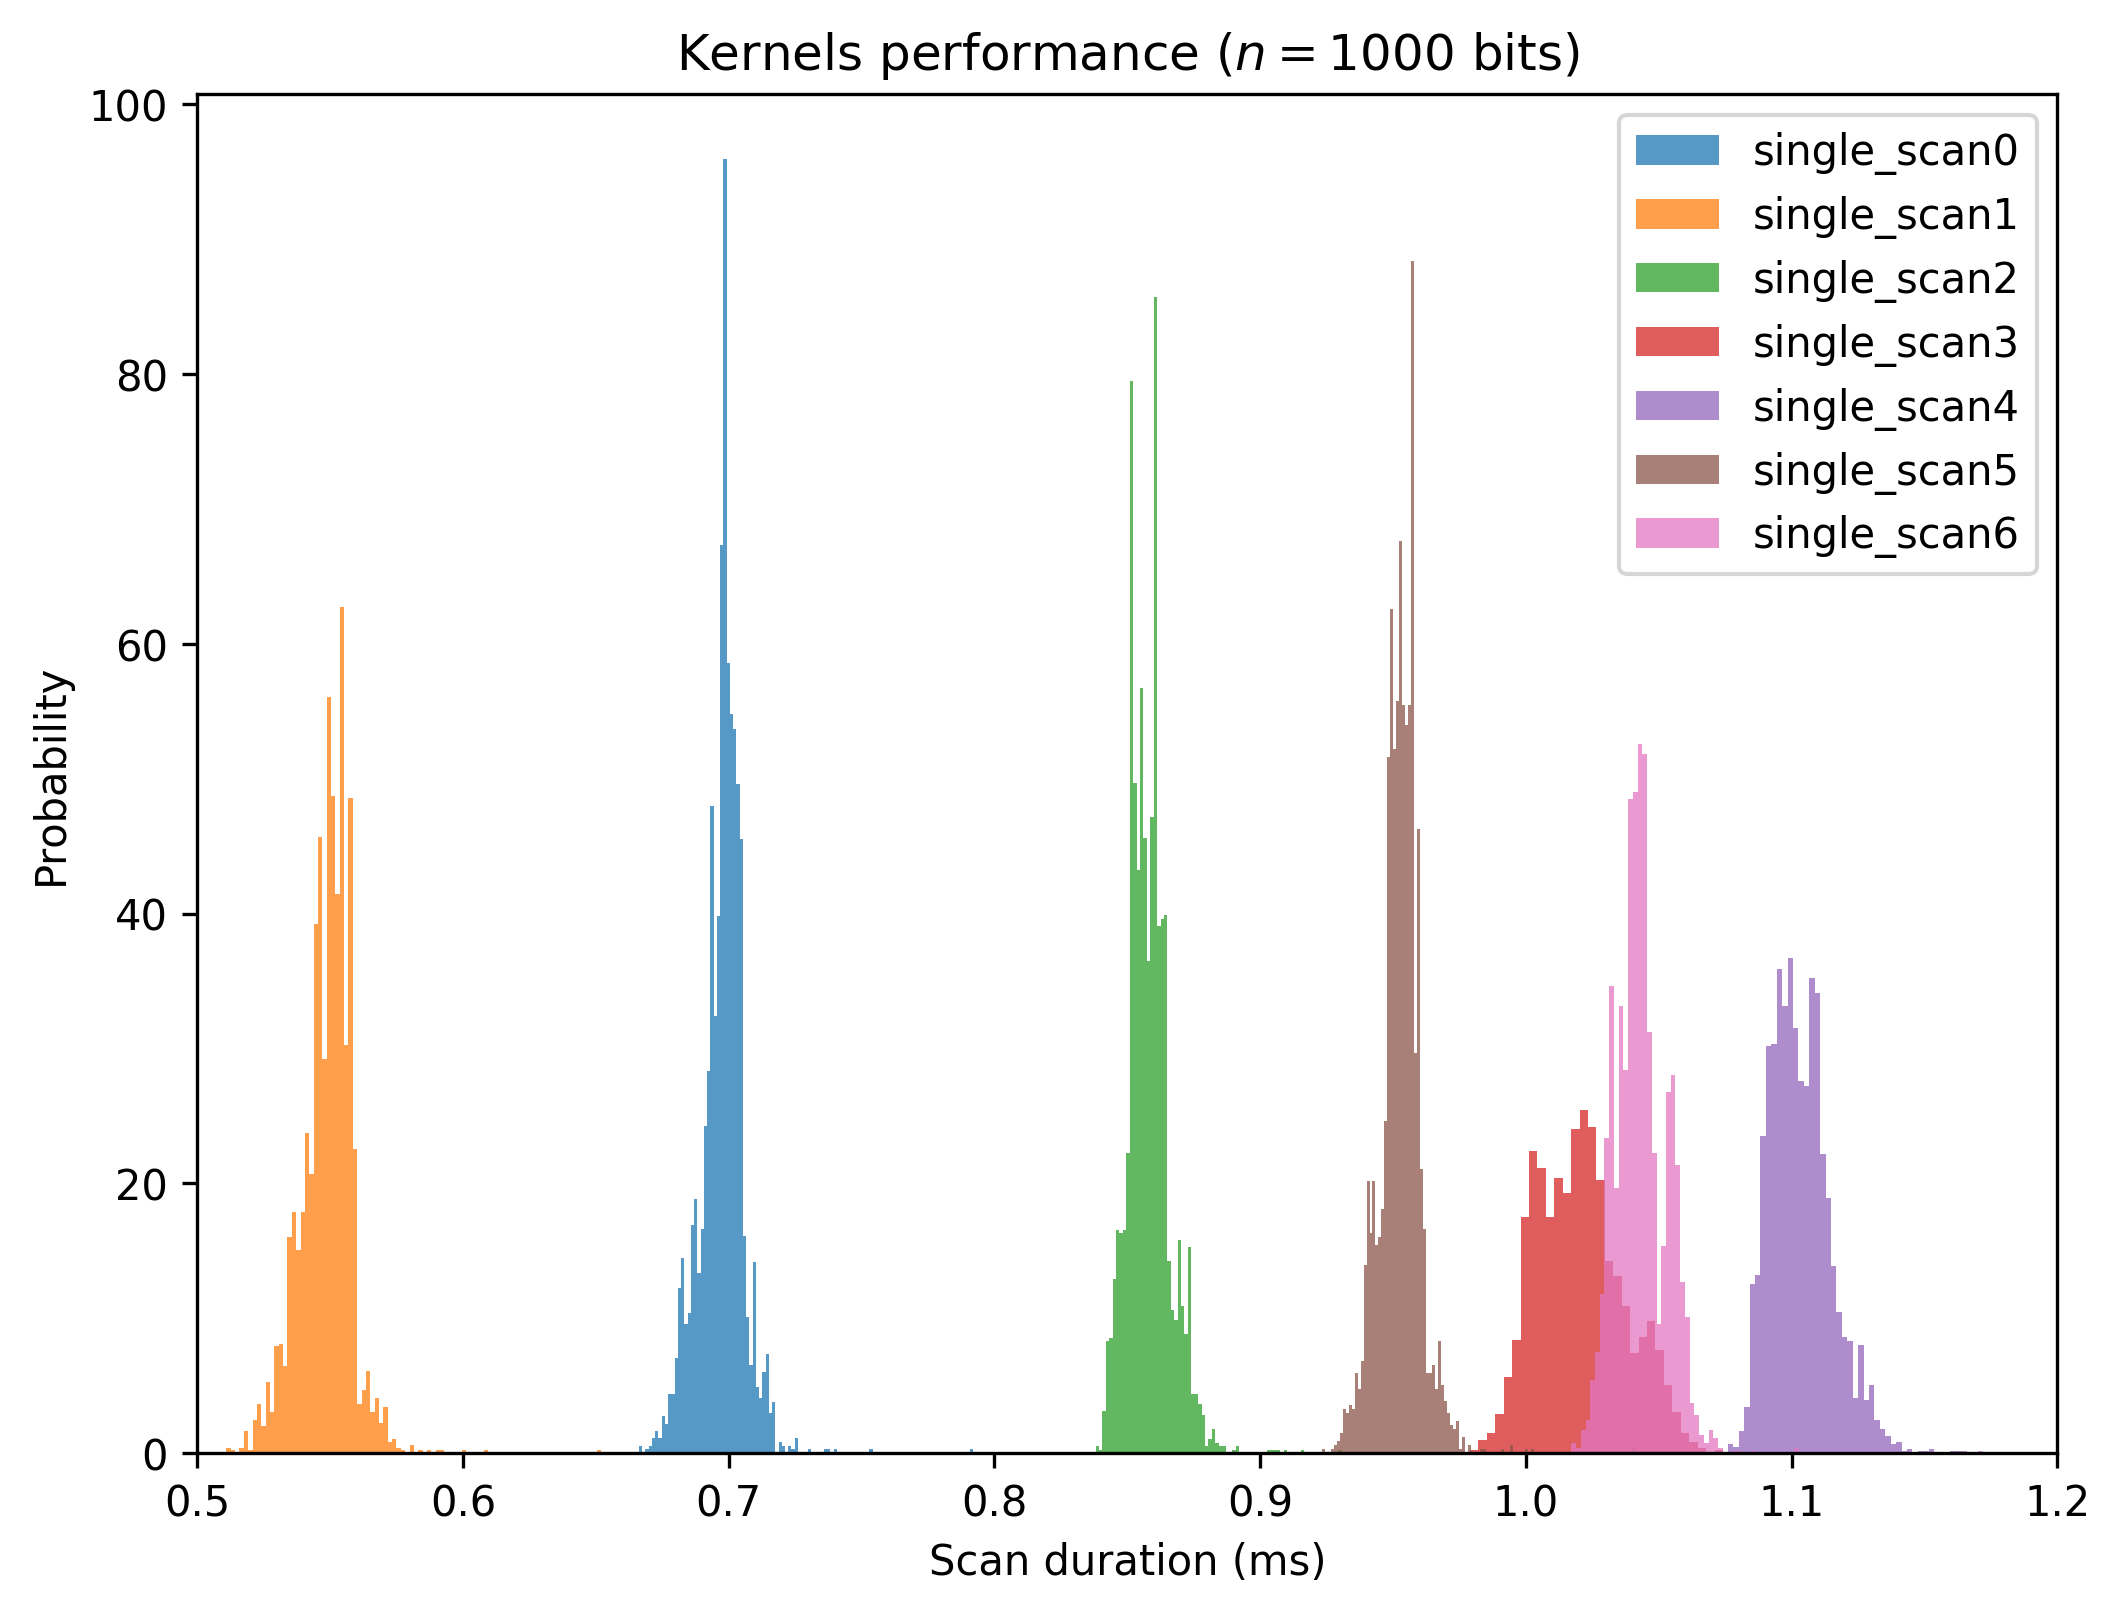
\includegraphics[width=0.7\textwidth]{images02/performance/ec2-p3-kernels-1000.png}}

\subfloat[$n=10,000$, $r=4805$, and $H=1,000,000$]{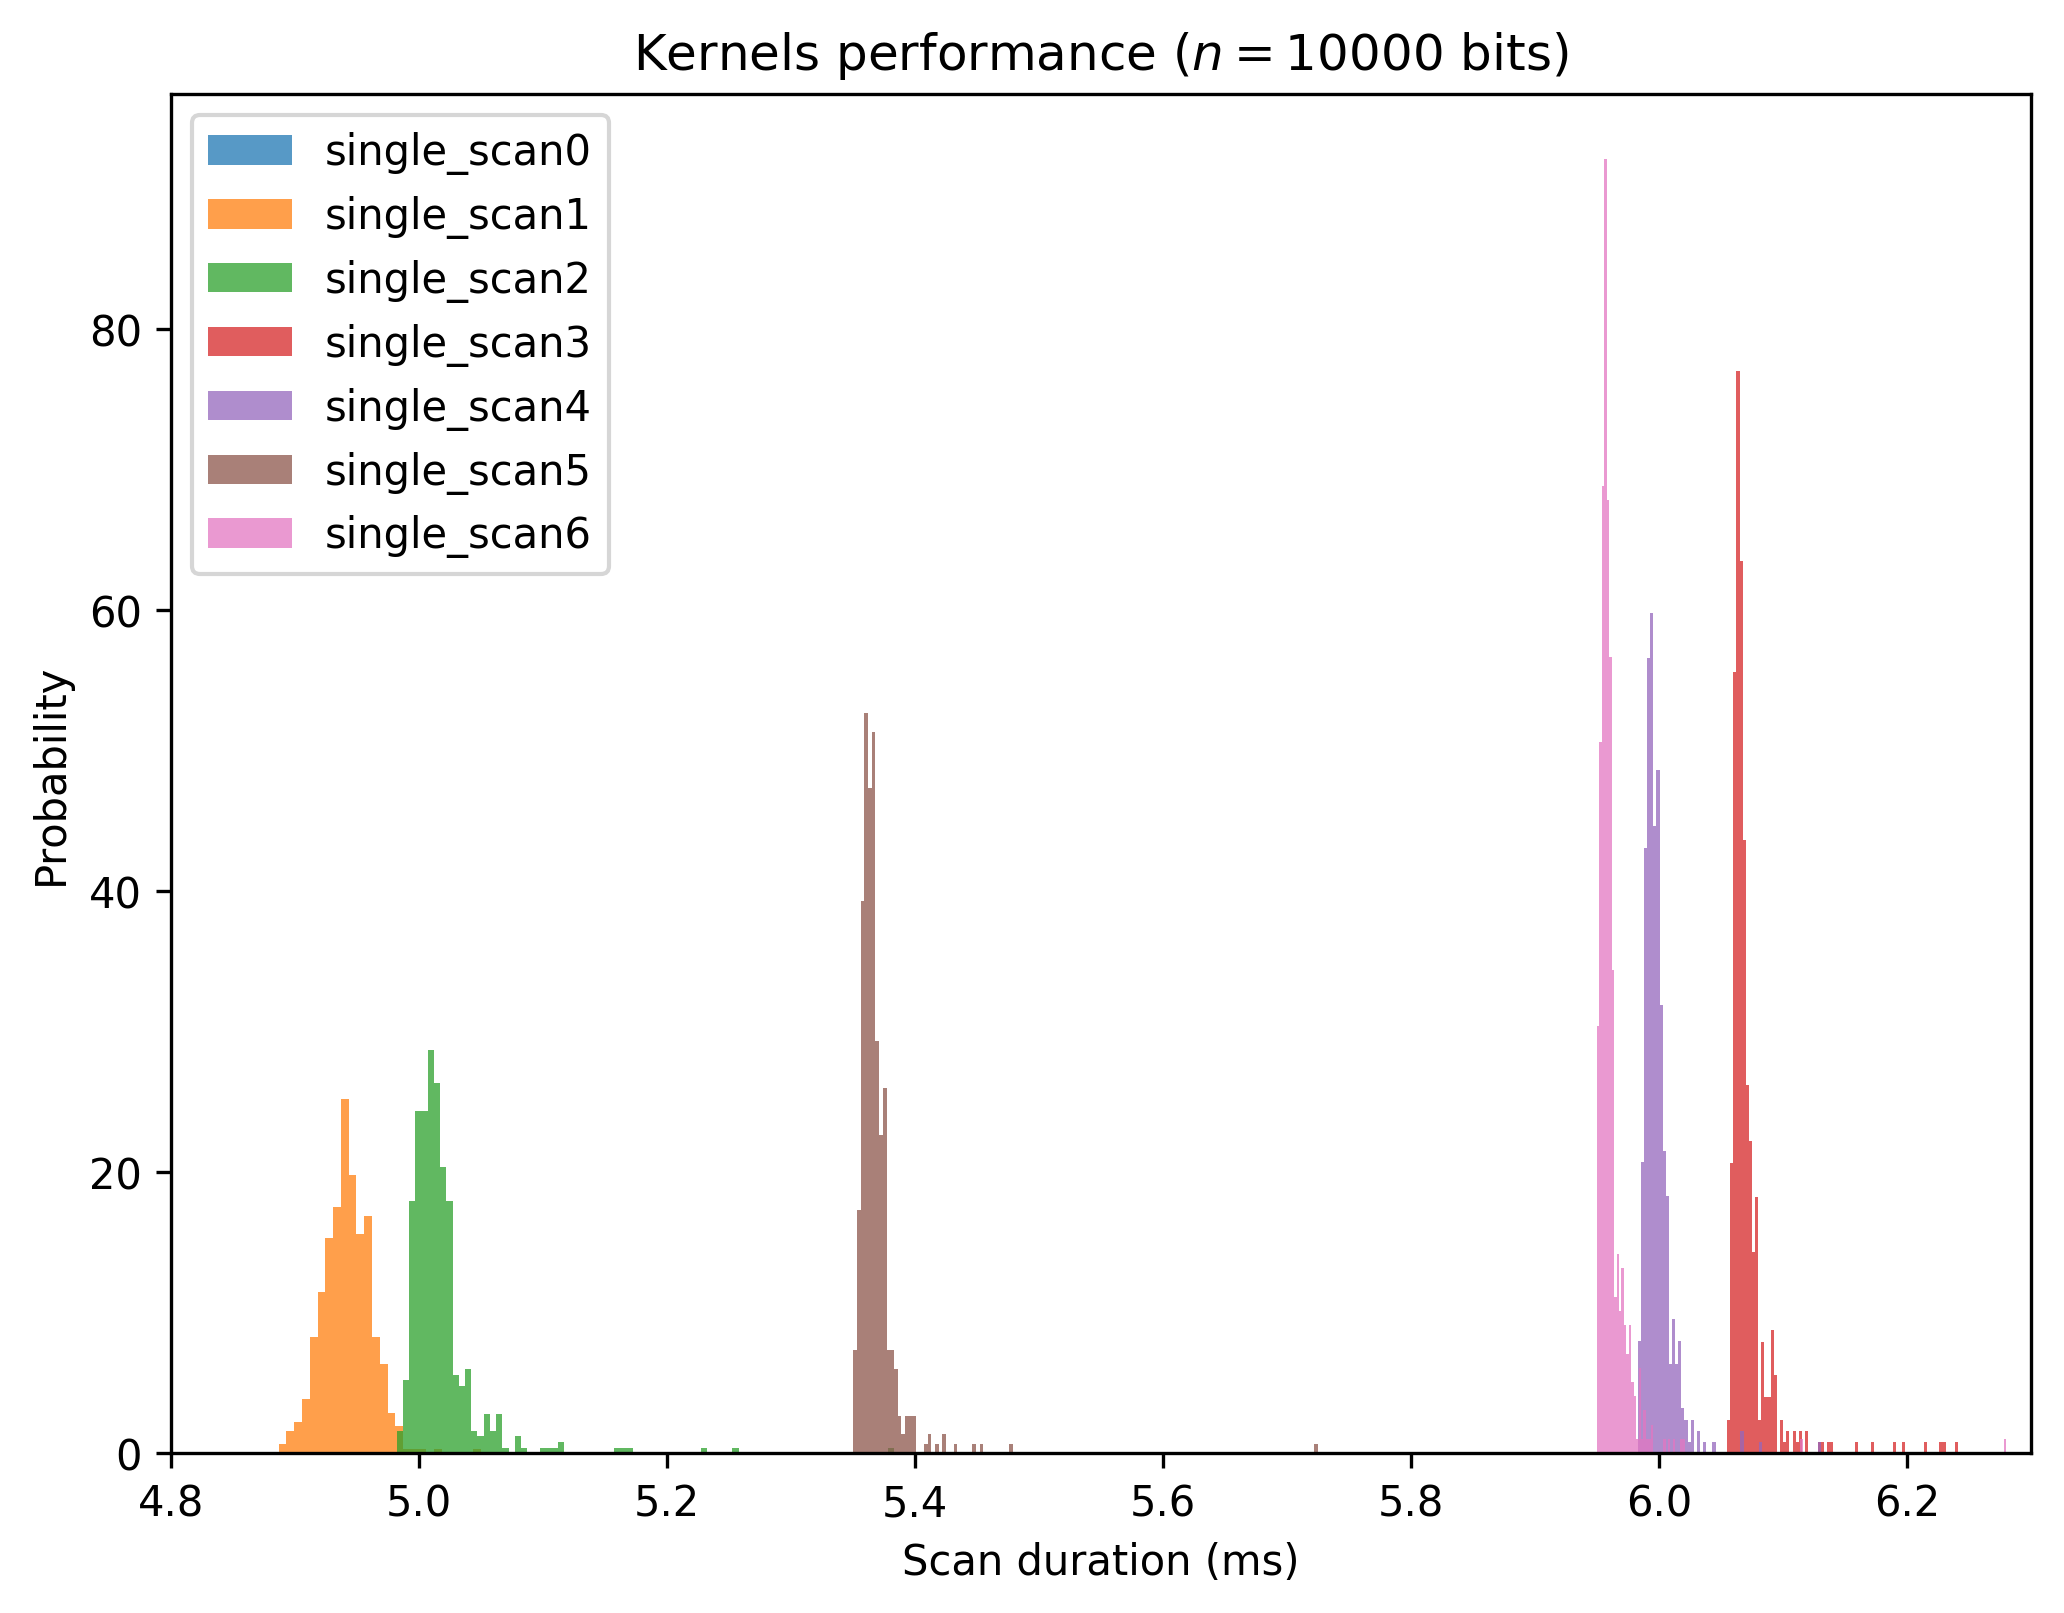
\includegraphics[width=0.7\textwidth]{images02/performance/ec2-p3-kernels-10k.png}}

\caption{Kernel comparisons for Amazon EC2 p3.2xlarge with Intel Xeon E5-2686v4 processor, 488GB DDR3 RAM, and NVIDIA Tesla V100 GPU.
\label{fig:perf-ec2-p3-kernels}}
\end{figure}

\begin{figure}[!htb]
\centering
\subfloat[$n=1,000$, $r=451$, and $H=1,000,000$]{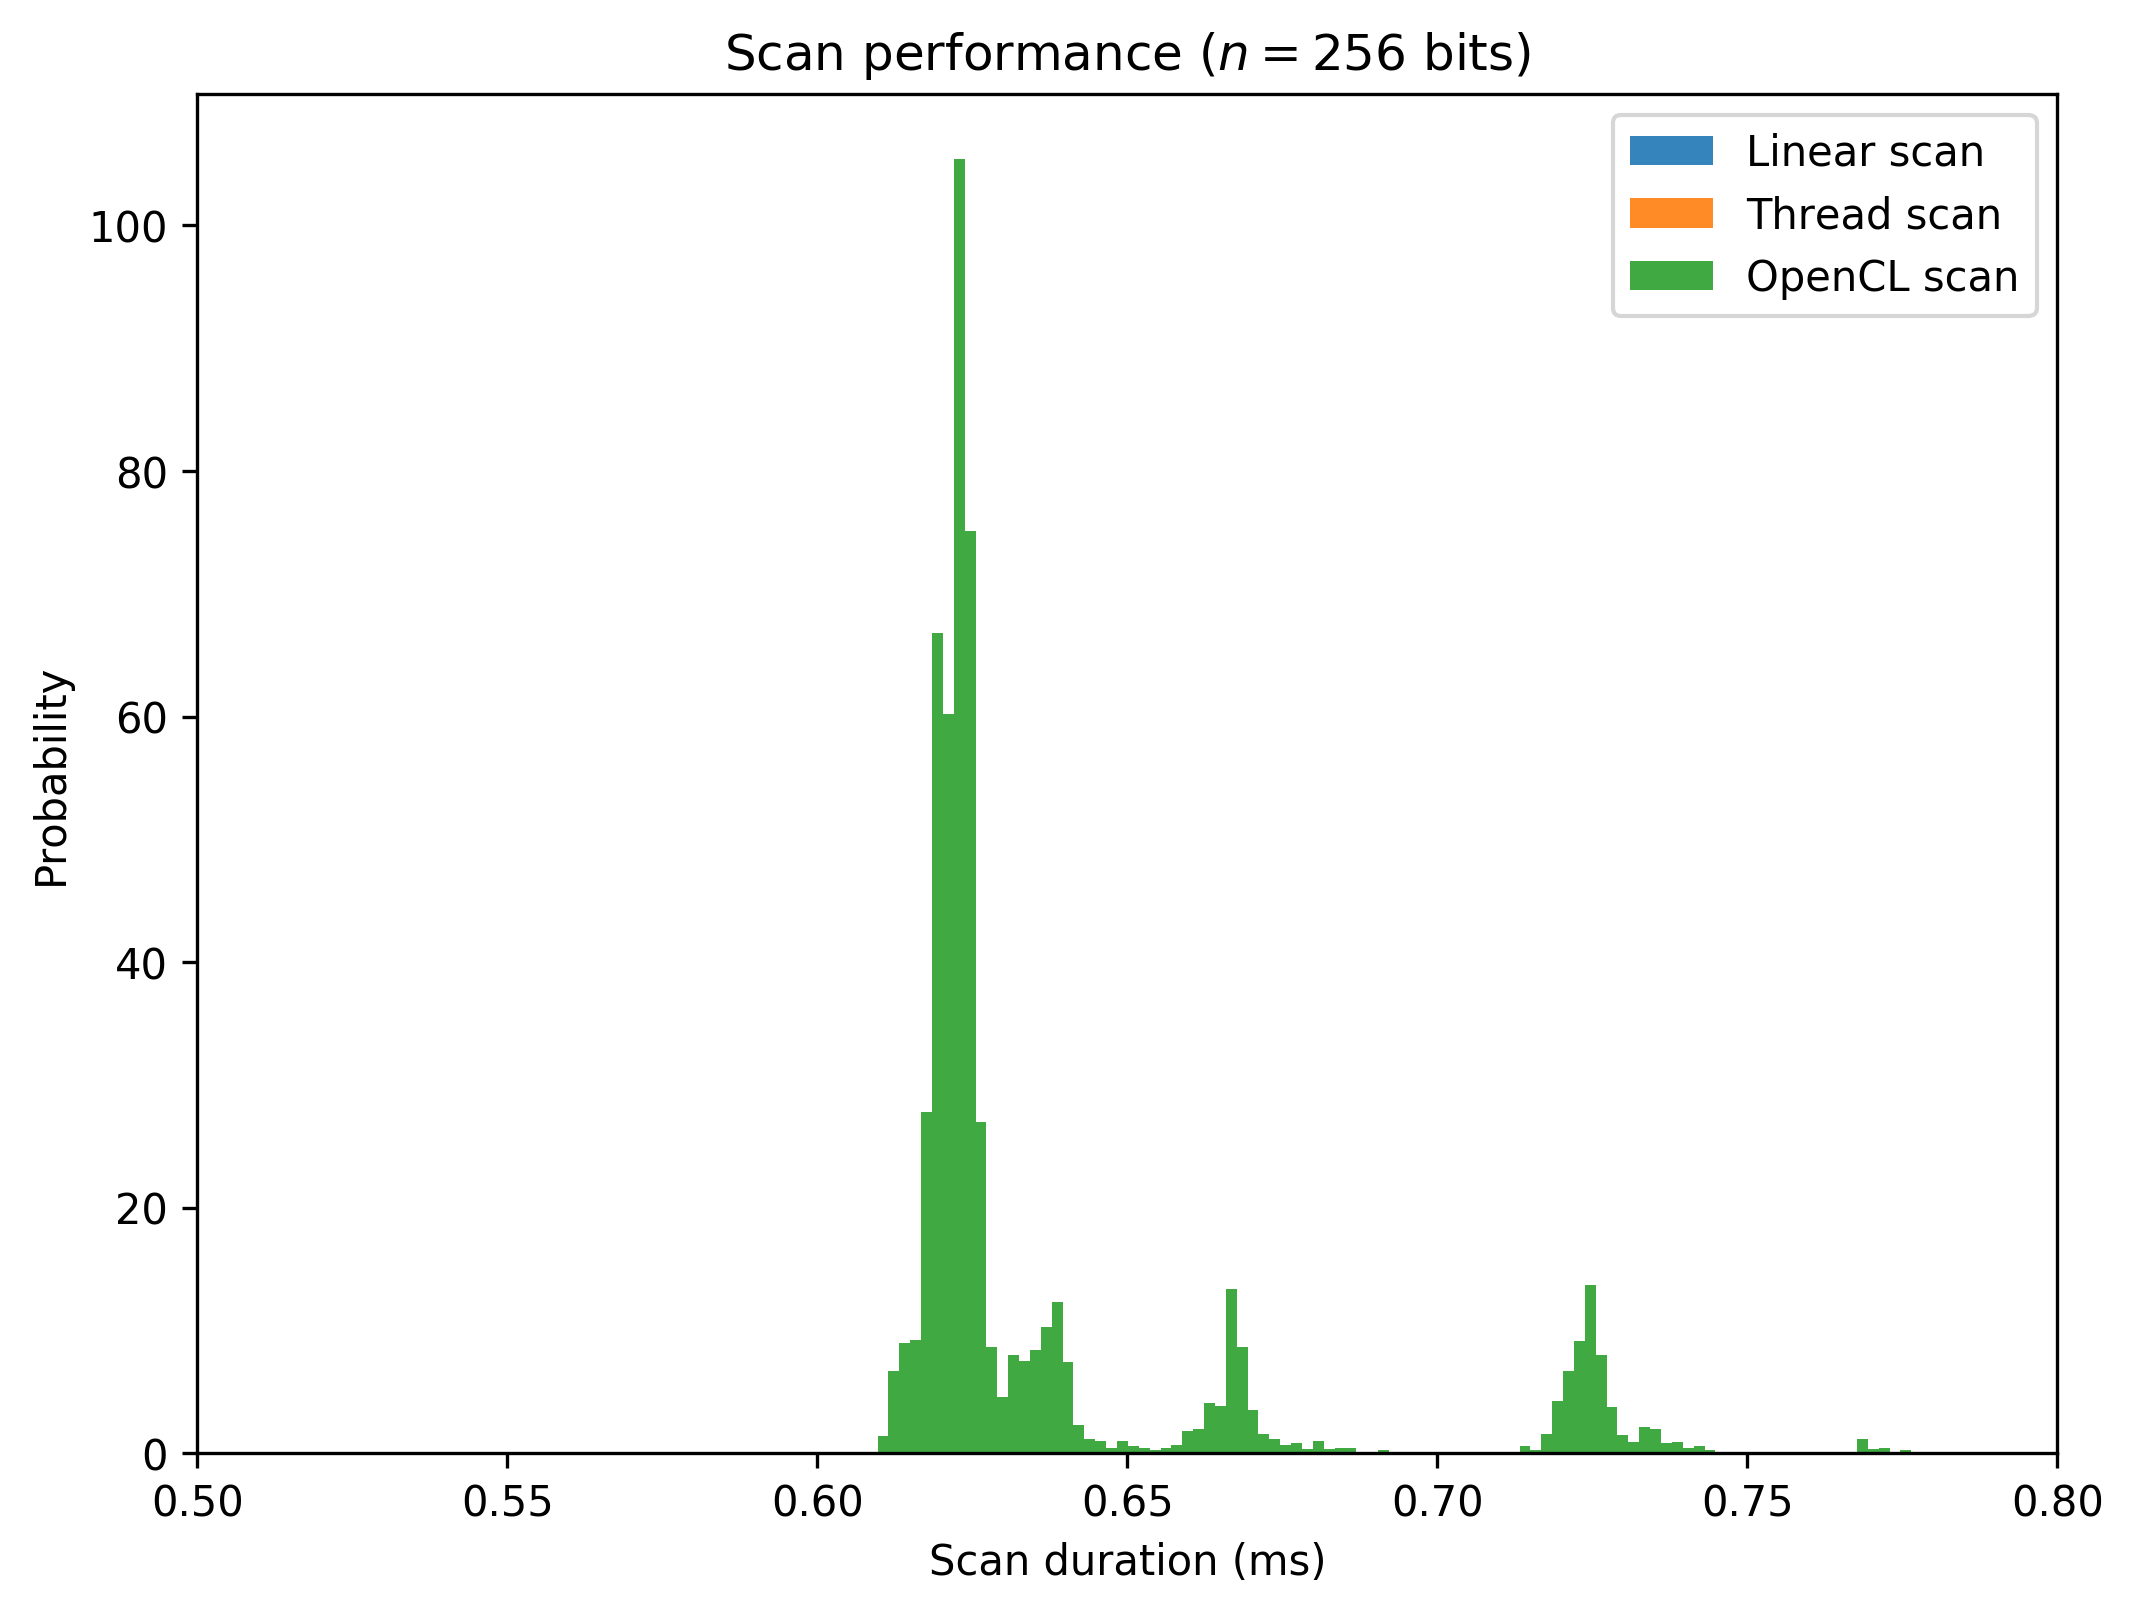
\includegraphics[width=0.7\textwidth]{images02/performance/ec2-p3-scan-256.png}}

\subfloat[$n=1,000$, $r=451$, and $H=1,000,000$]{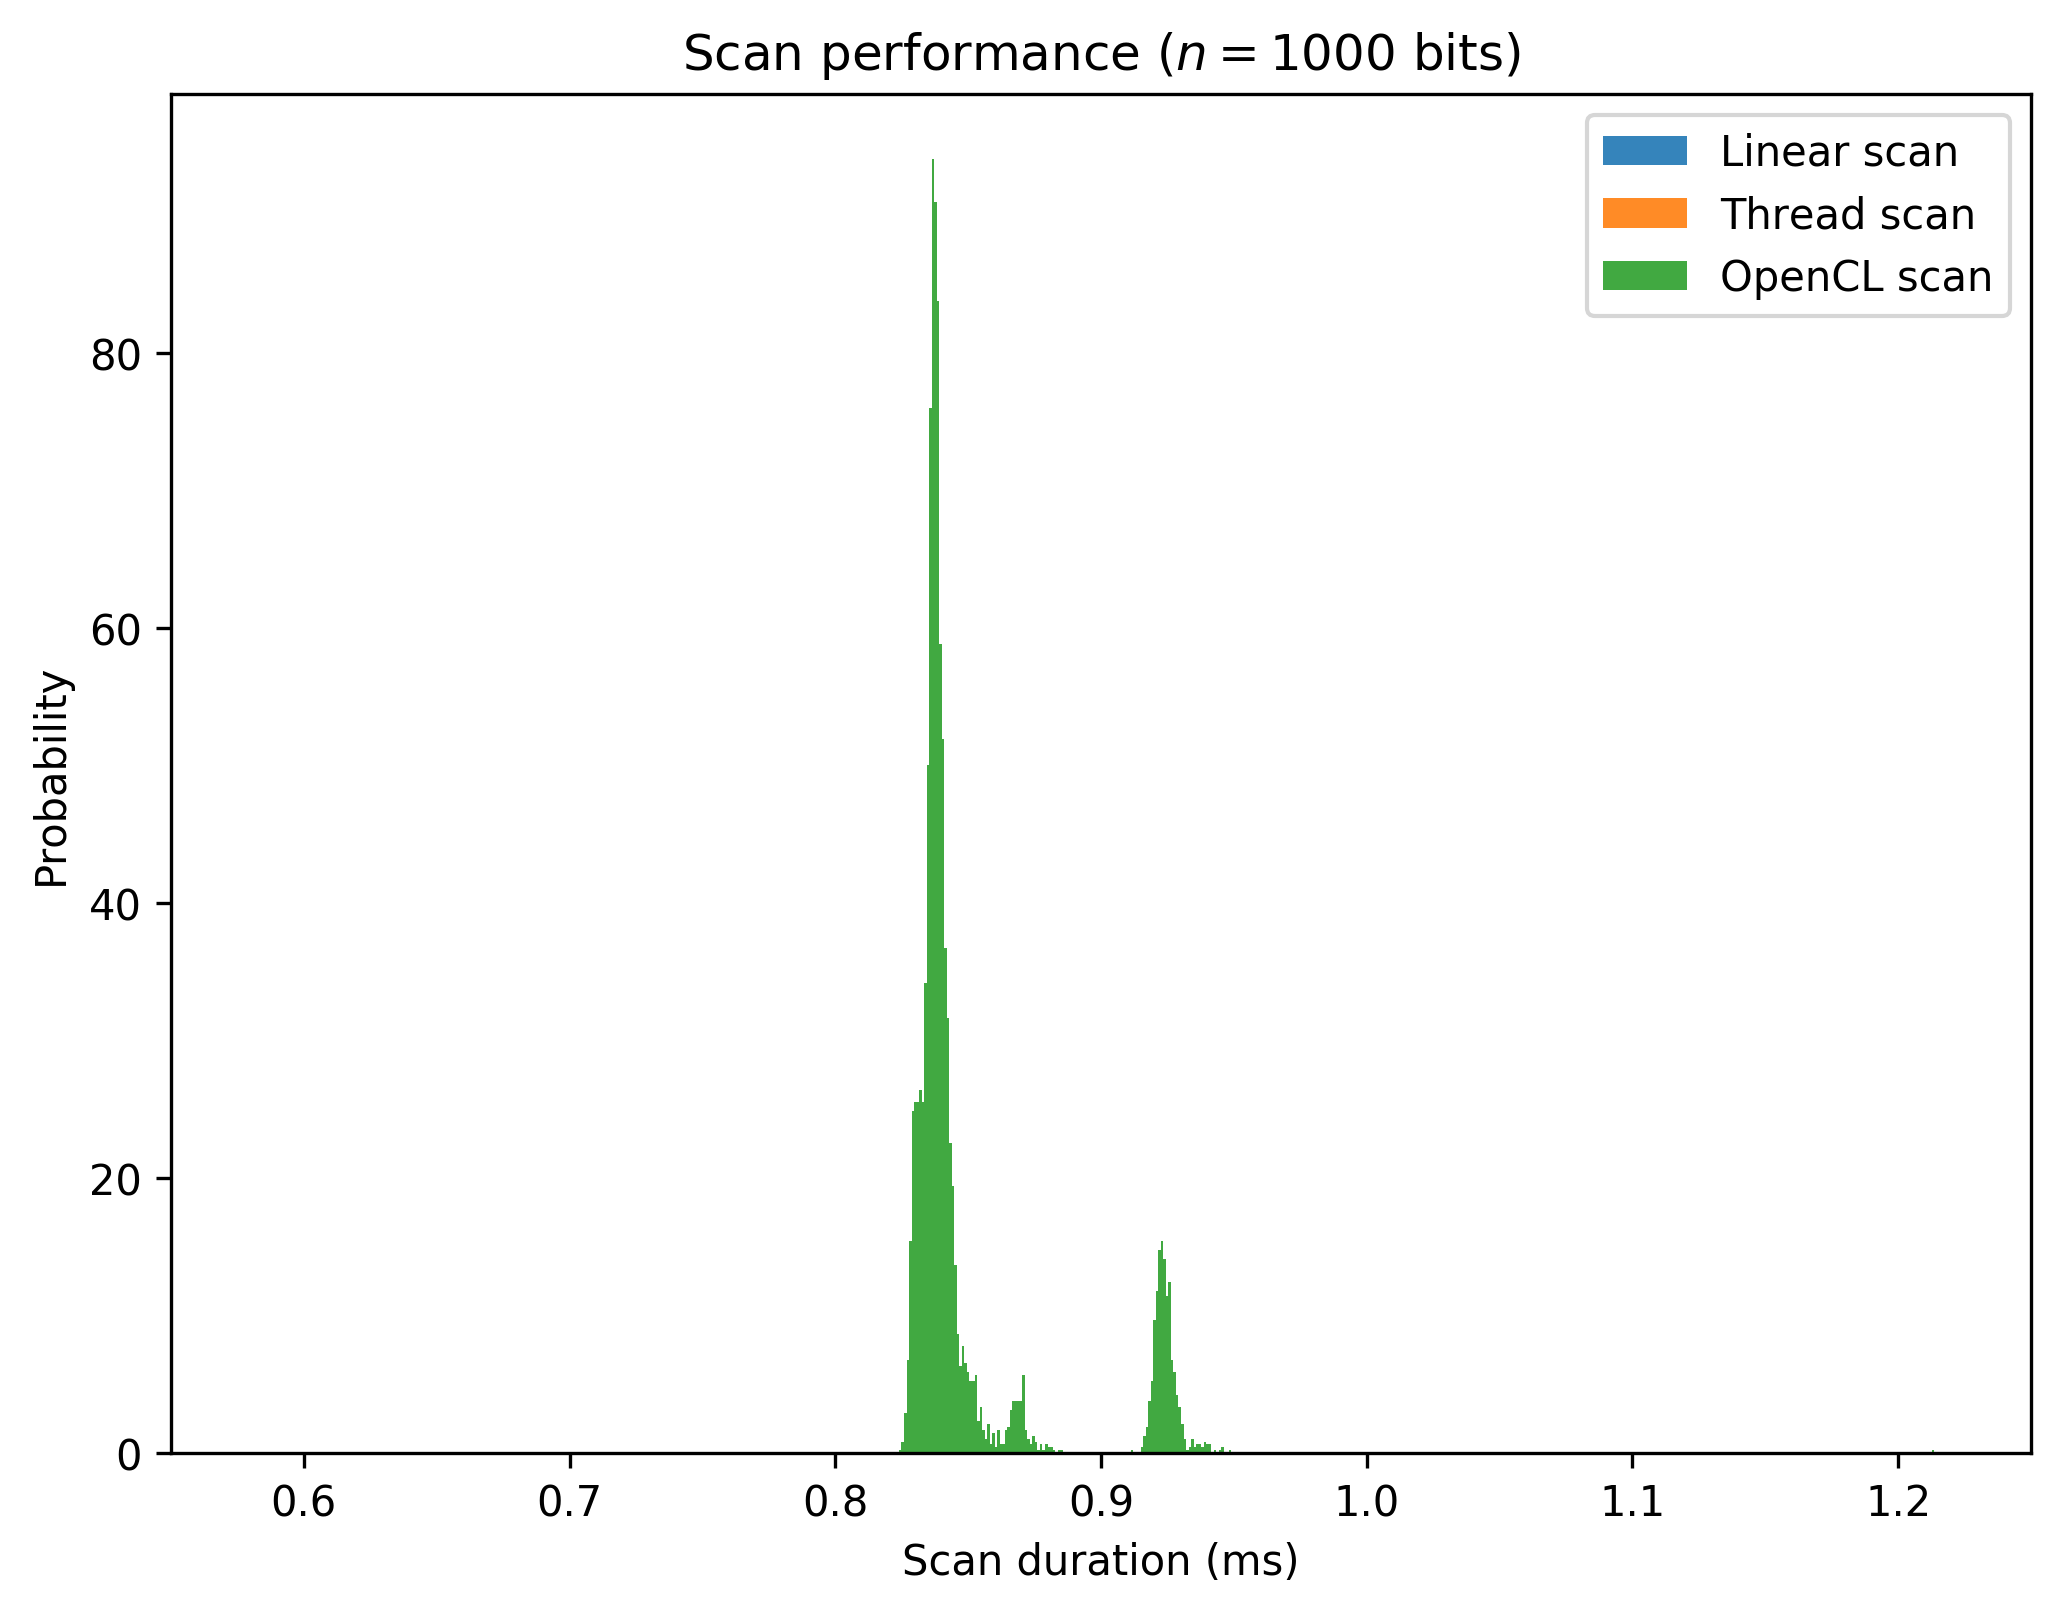
\includegraphics[width=0.7\textwidth]{images02/performance/ec2-p3-scan-1000.png}}

\subfloat[$n=10,000$, $r=4805$, and $H=1,000,000$]{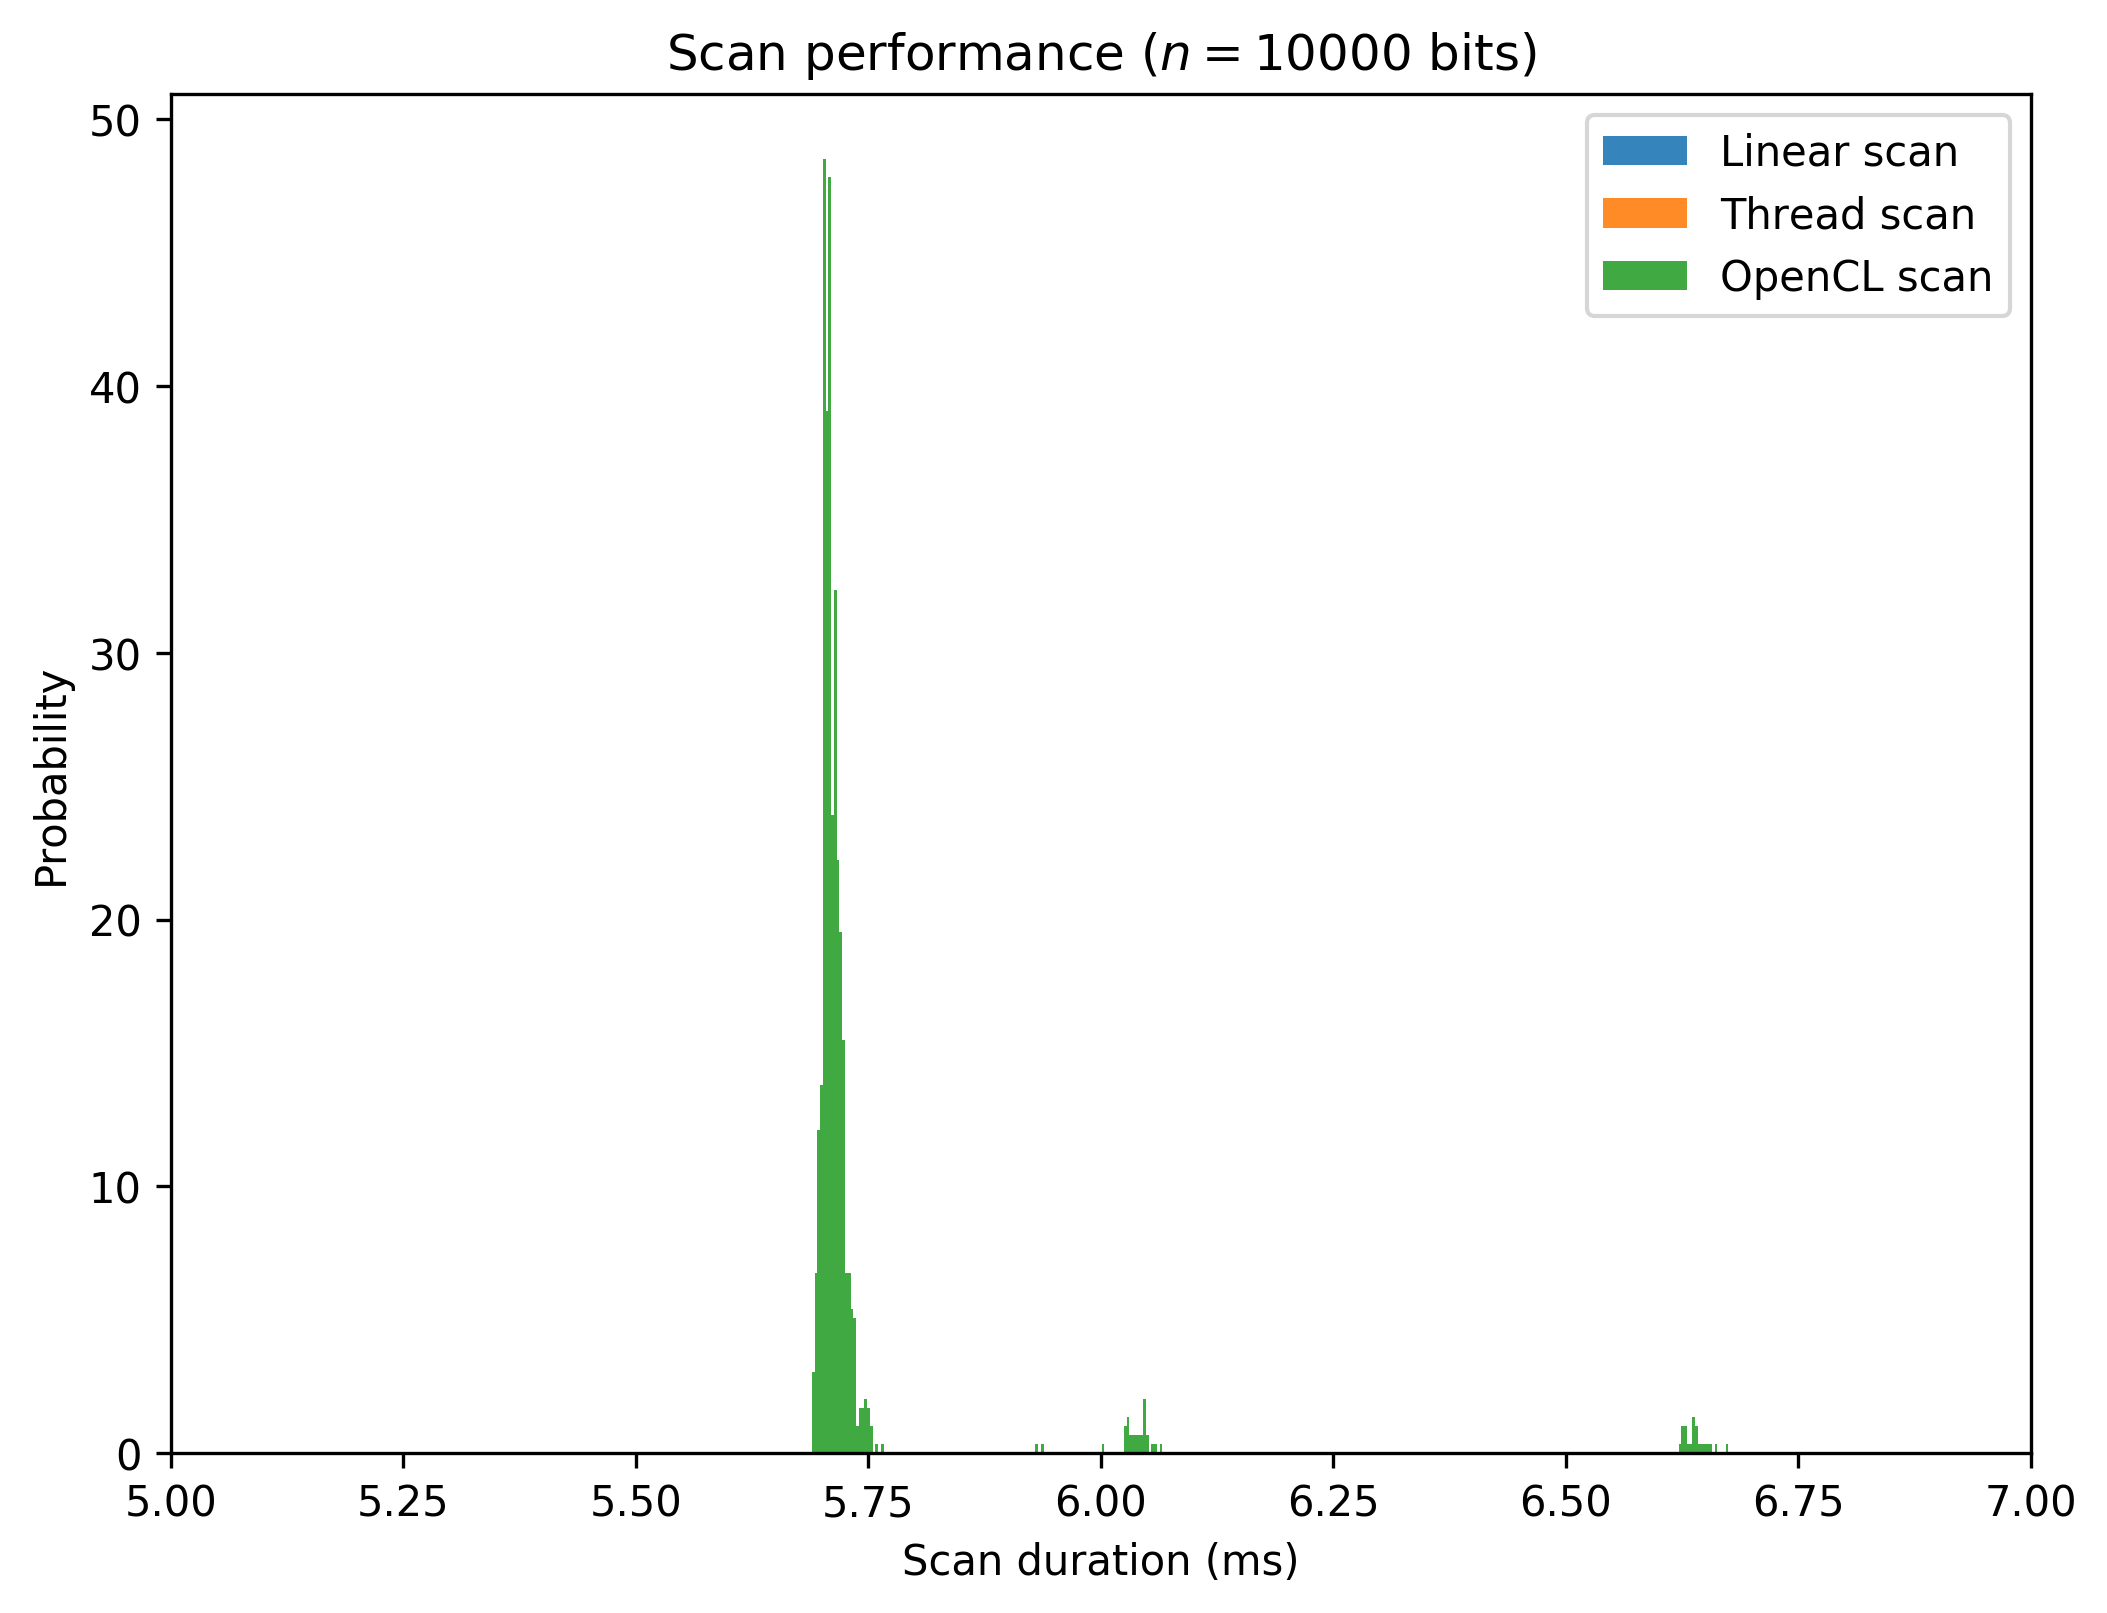
\includegraphics[width=0.7\textwidth]{images02/performance/ec2-p3-scan-10k.png}}

\caption{Scanner comparisons for Amazon EC2 p3.2xlarge with Intel Xeon E5-2686v4 processor, 488GB DDR3 RAM, and NVIDIA Tesla V100 GPU.
\label{fig:perf-ec2-p3-scanners}}
\end{figure}


\begin{figure}[!htb]
\centering
\subfloat[$n=1,000$, $r=451$, and $H=1,000,000$]{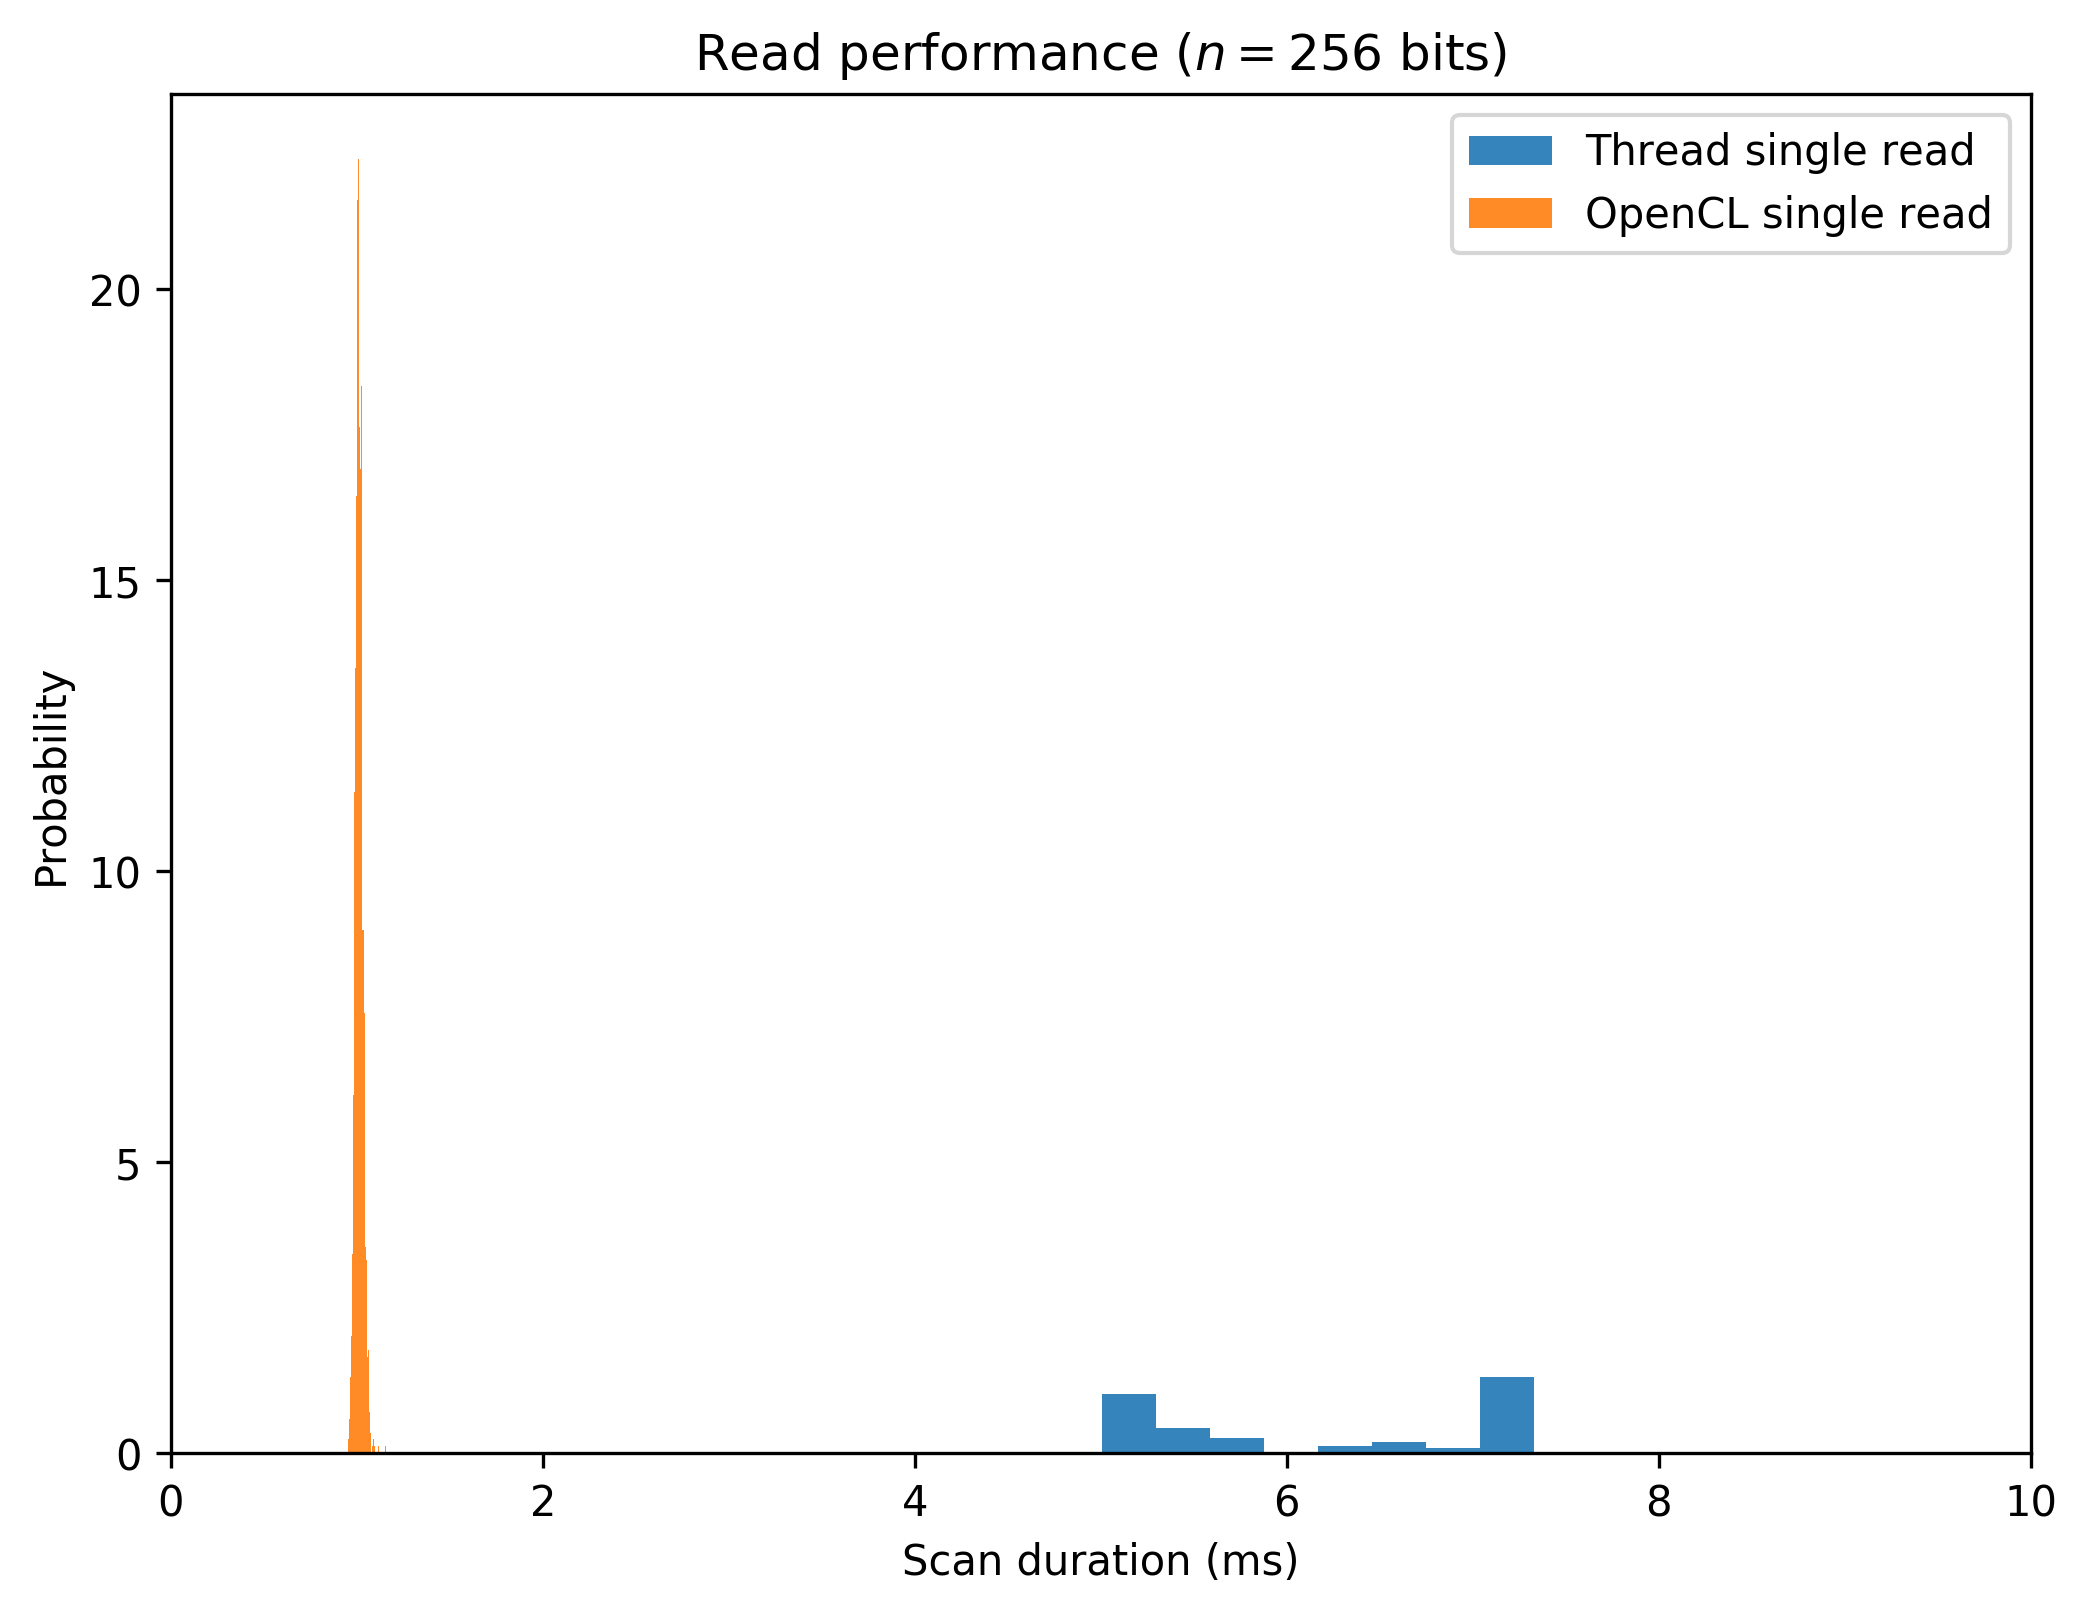
\includegraphics[width=0.7\textwidth]{images02/performance/ec2-p3-read-256.png}}

\subfloat[$n=1,000$, $r=451$, and $H=1,000,000$]{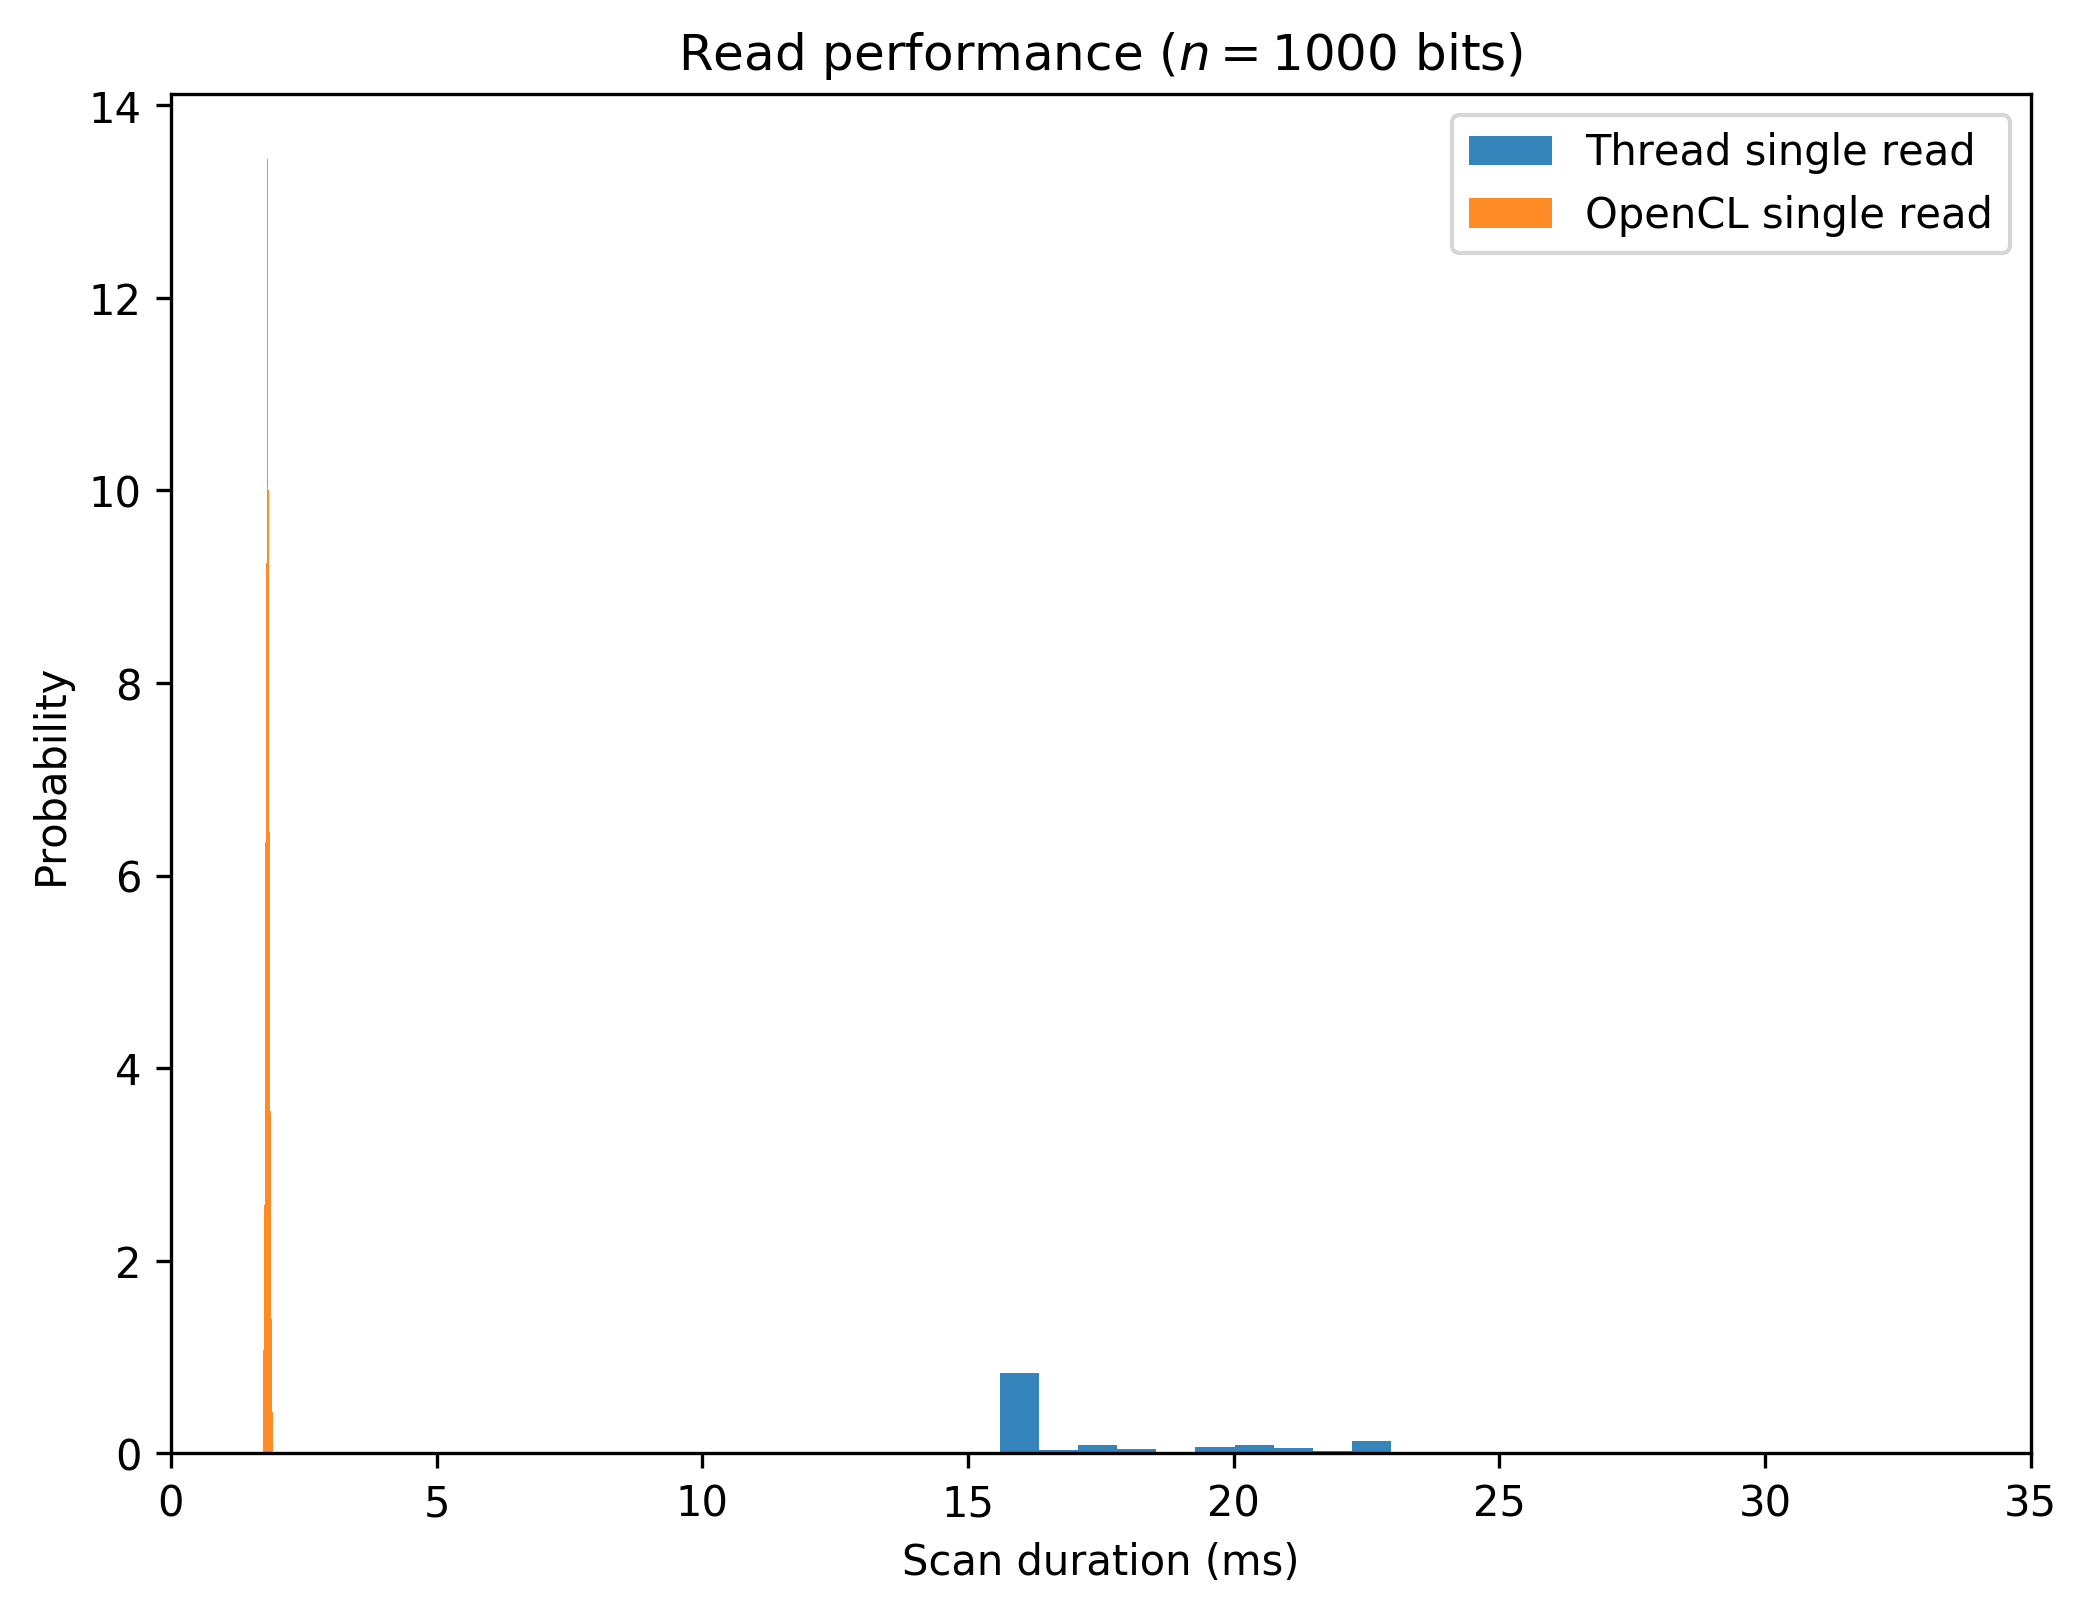
\includegraphics[width=0.7\textwidth]{images02/performance/ec2-p3-read-1000.png}}

\subfloat[$n=10,000$, $r=4805$, and $H=1,000,000$]{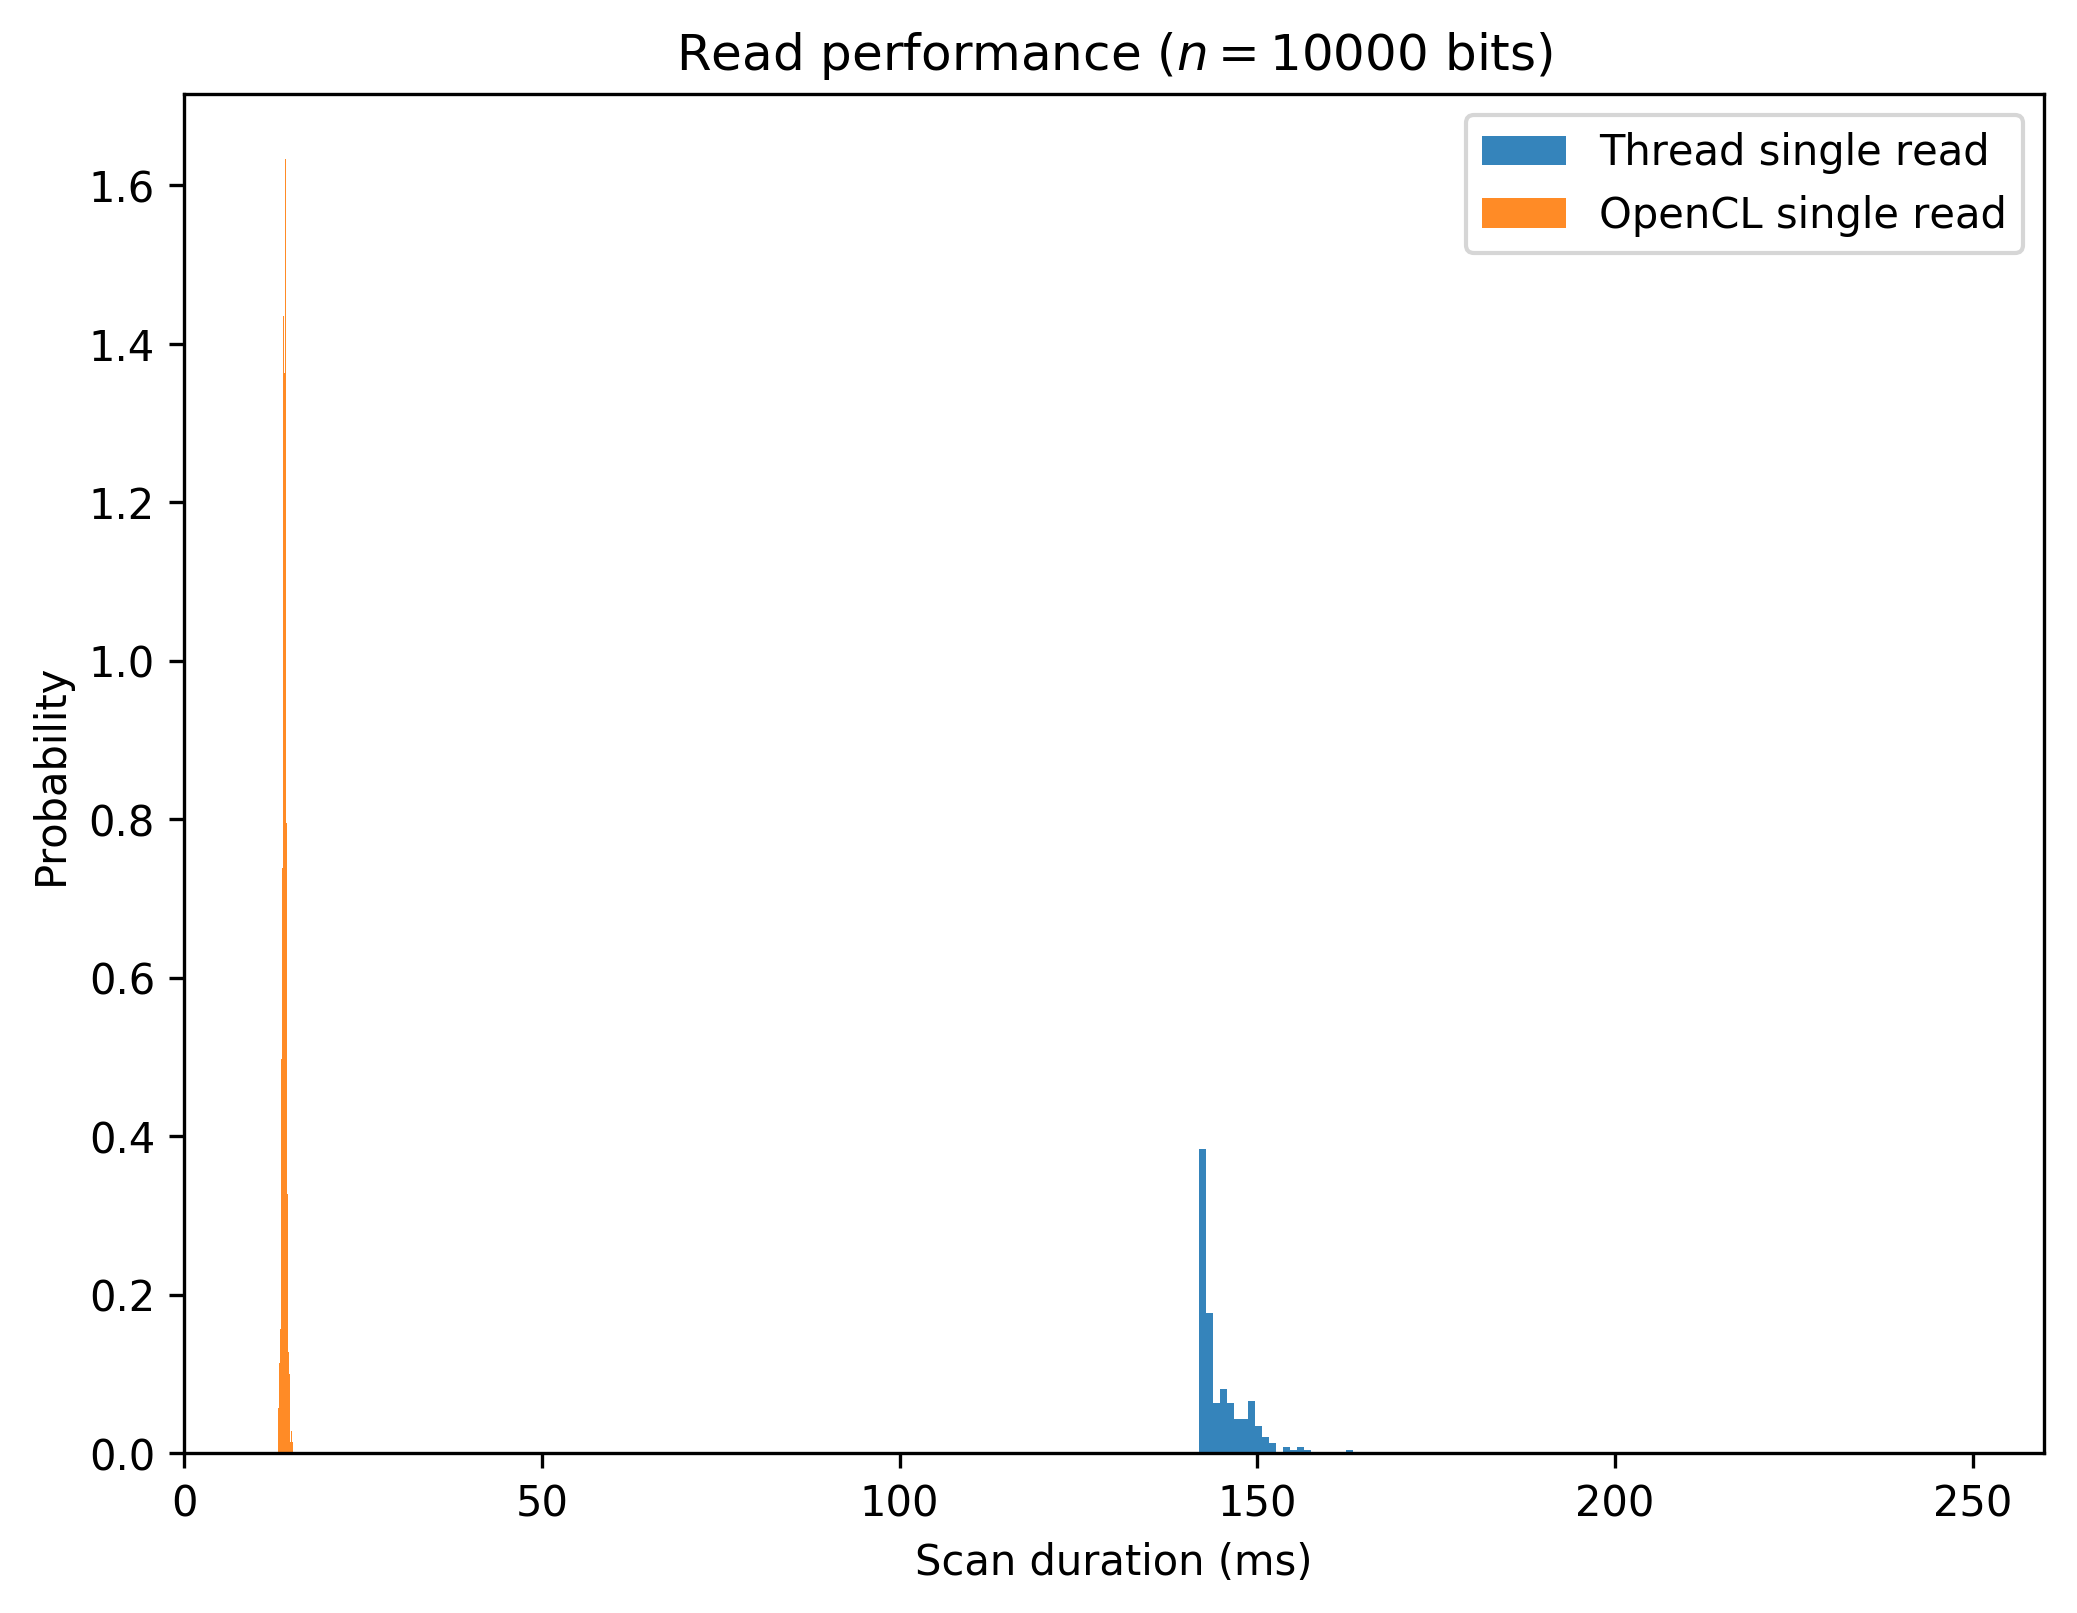
\includegraphics[width=0.7\textwidth]{images02/performance/ec2-p3-read-10k.png}}

\caption{Read operation comparisons for Amazon EC2 p3.2xlarge with Intel Xeon E5-2686v4 processor, 488GB DDR3 RAM, and NVIDIA Tesla V100 GPU.
\label{fig:perf-ec2-p3-read}}
\end{figure}

\begin{figure}[!htb]
\centering
\subfloat[$n=1,000$, $r=451$, and $H=1,000,000$]{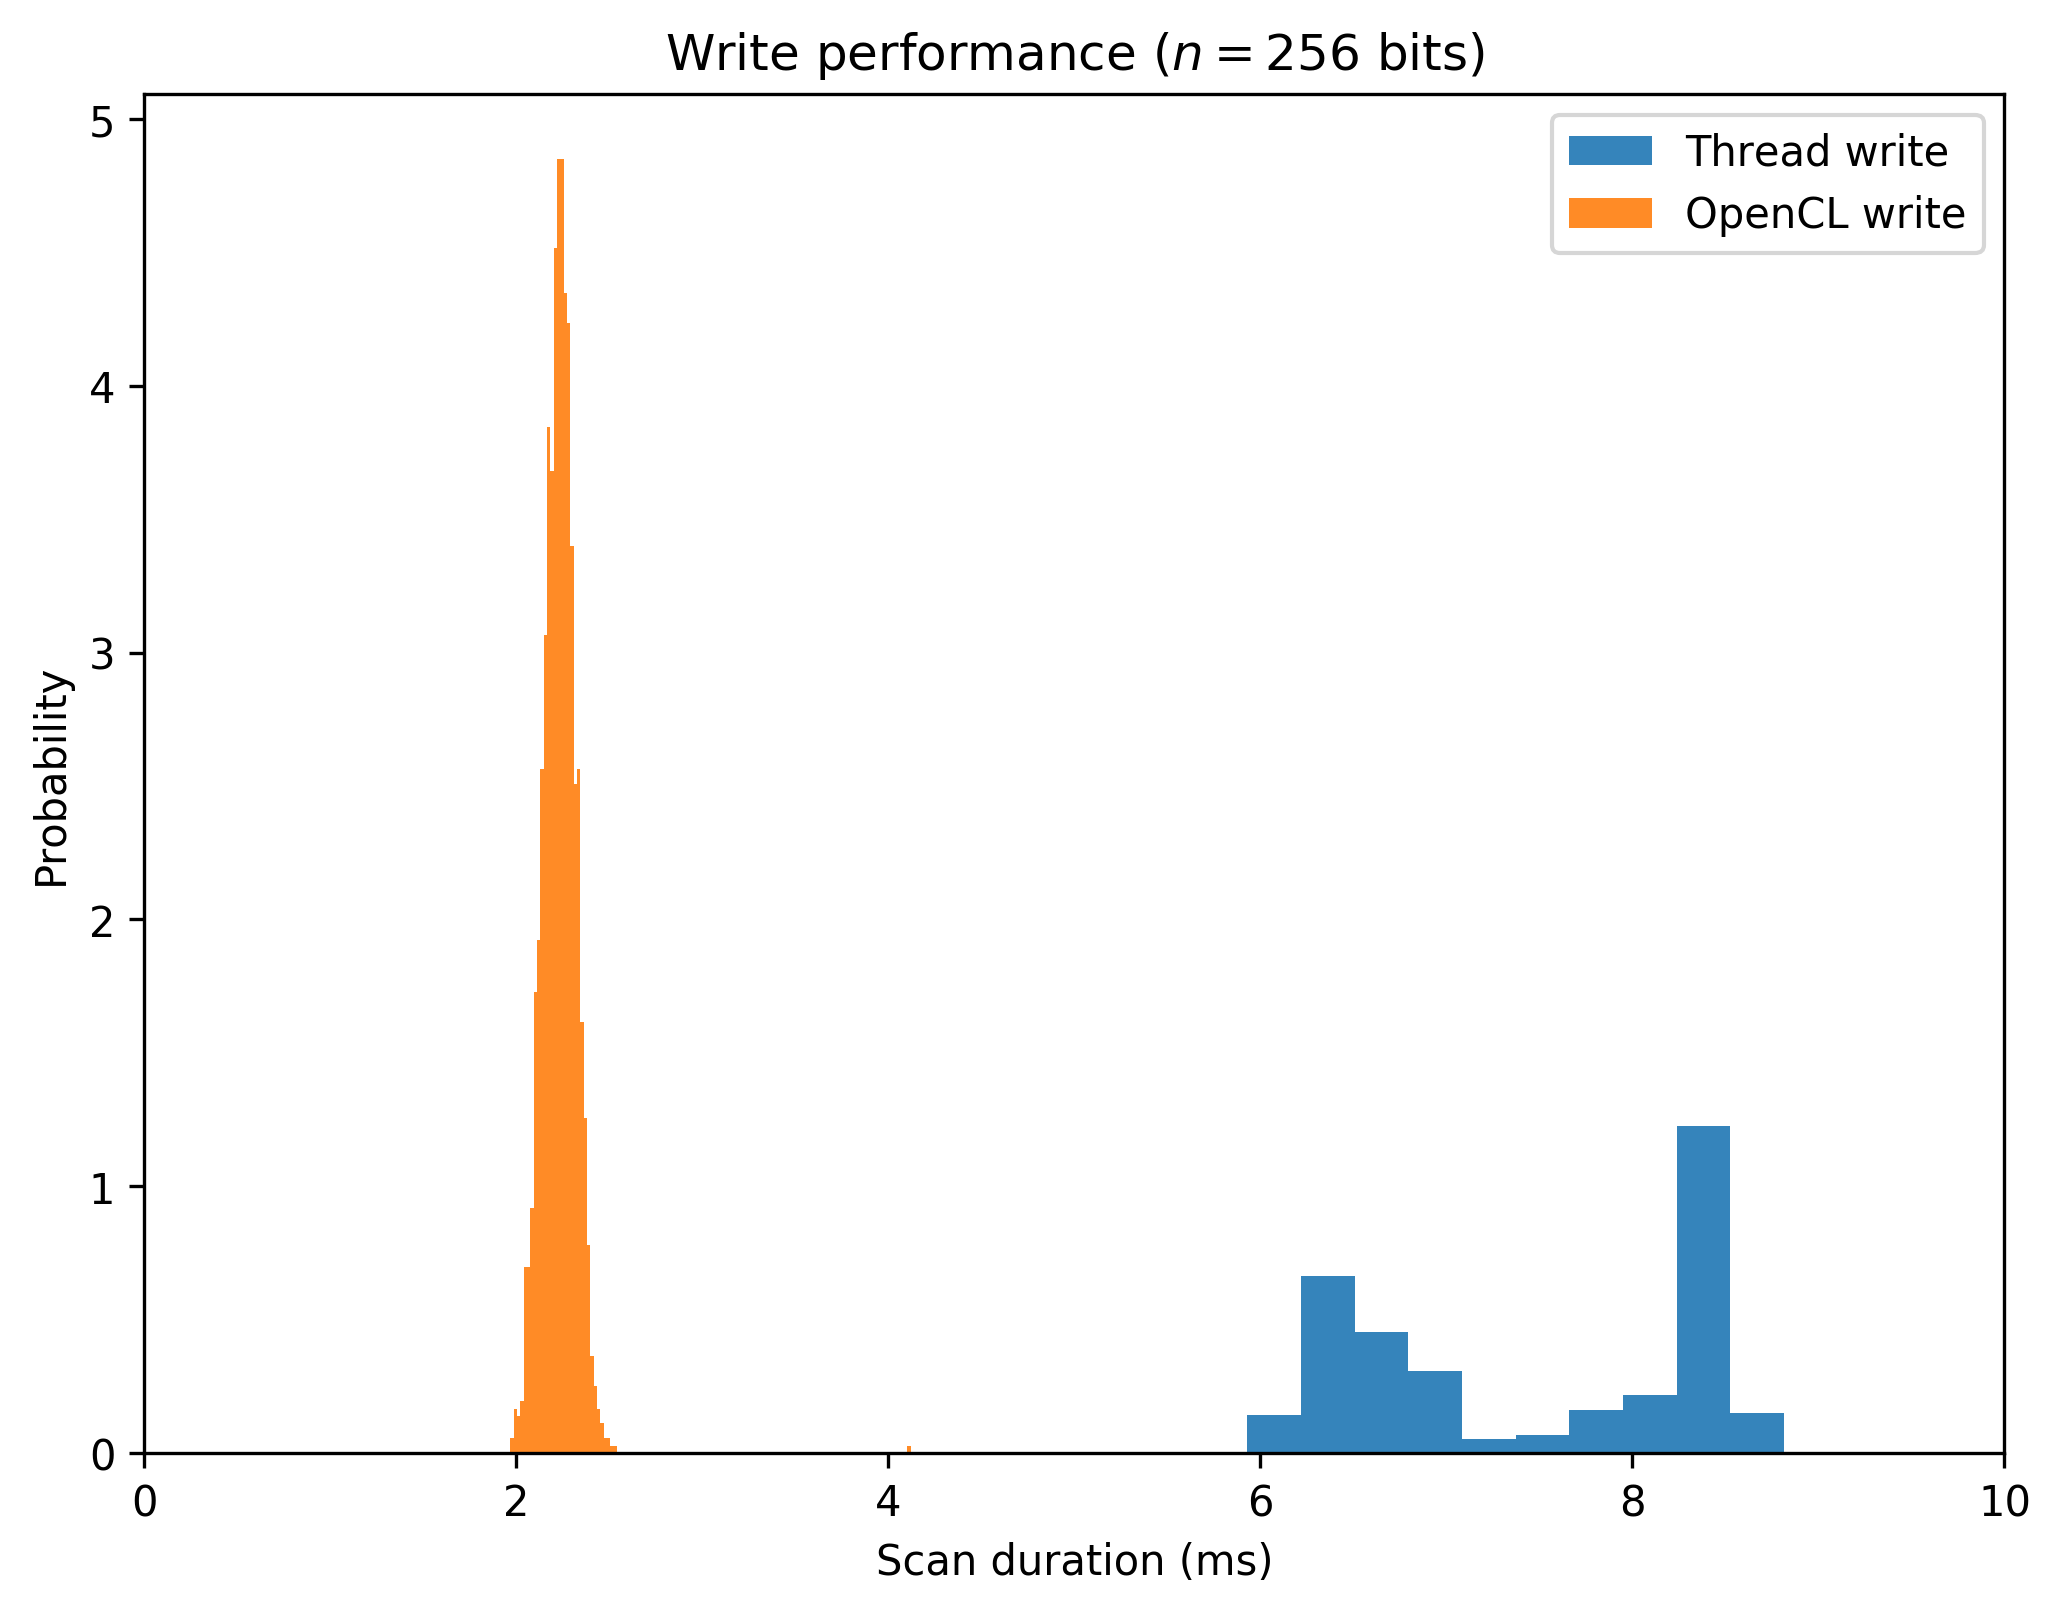
\includegraphics[width=0.7\textwidth]{images02/performance/ec2-p3-write-256.png}}

\subfloat[$n=1,000$, $r=451$, and $H=1,000,000$]{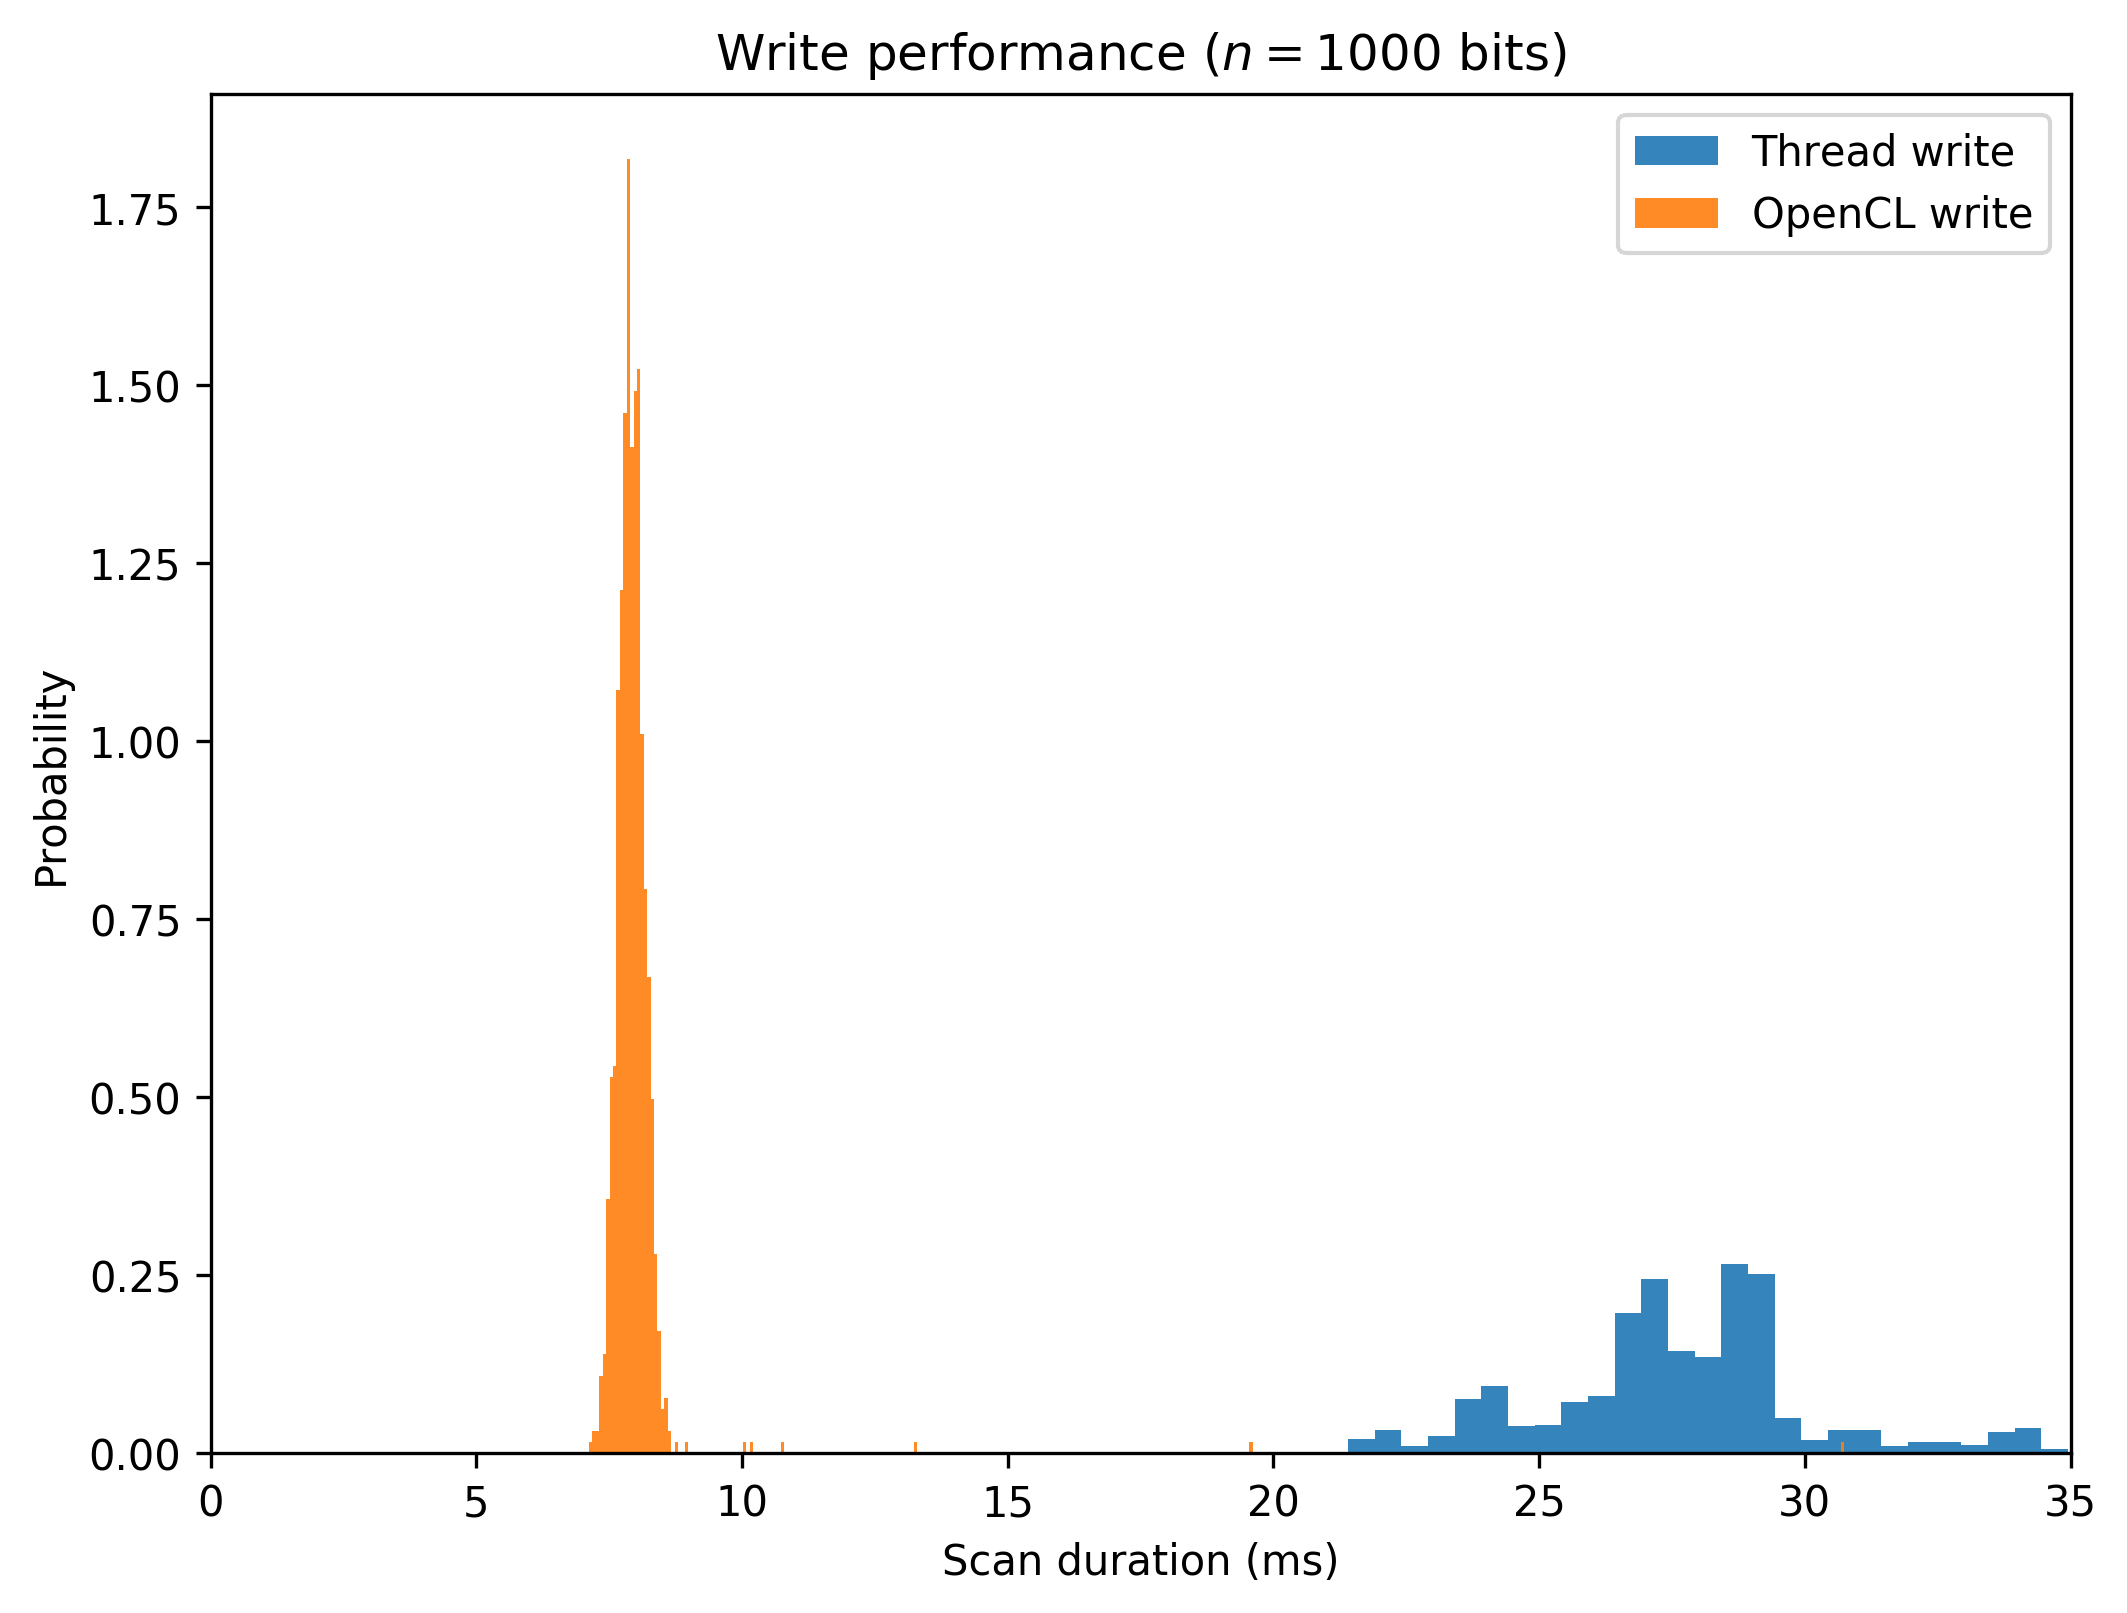
\includegraphics[width=0.7\textwidth]{images02/performance/ec2-p3-write-1000.png}}

\subfloat[$n=10,000$, $r=4805$, and $H=1,000,000$]{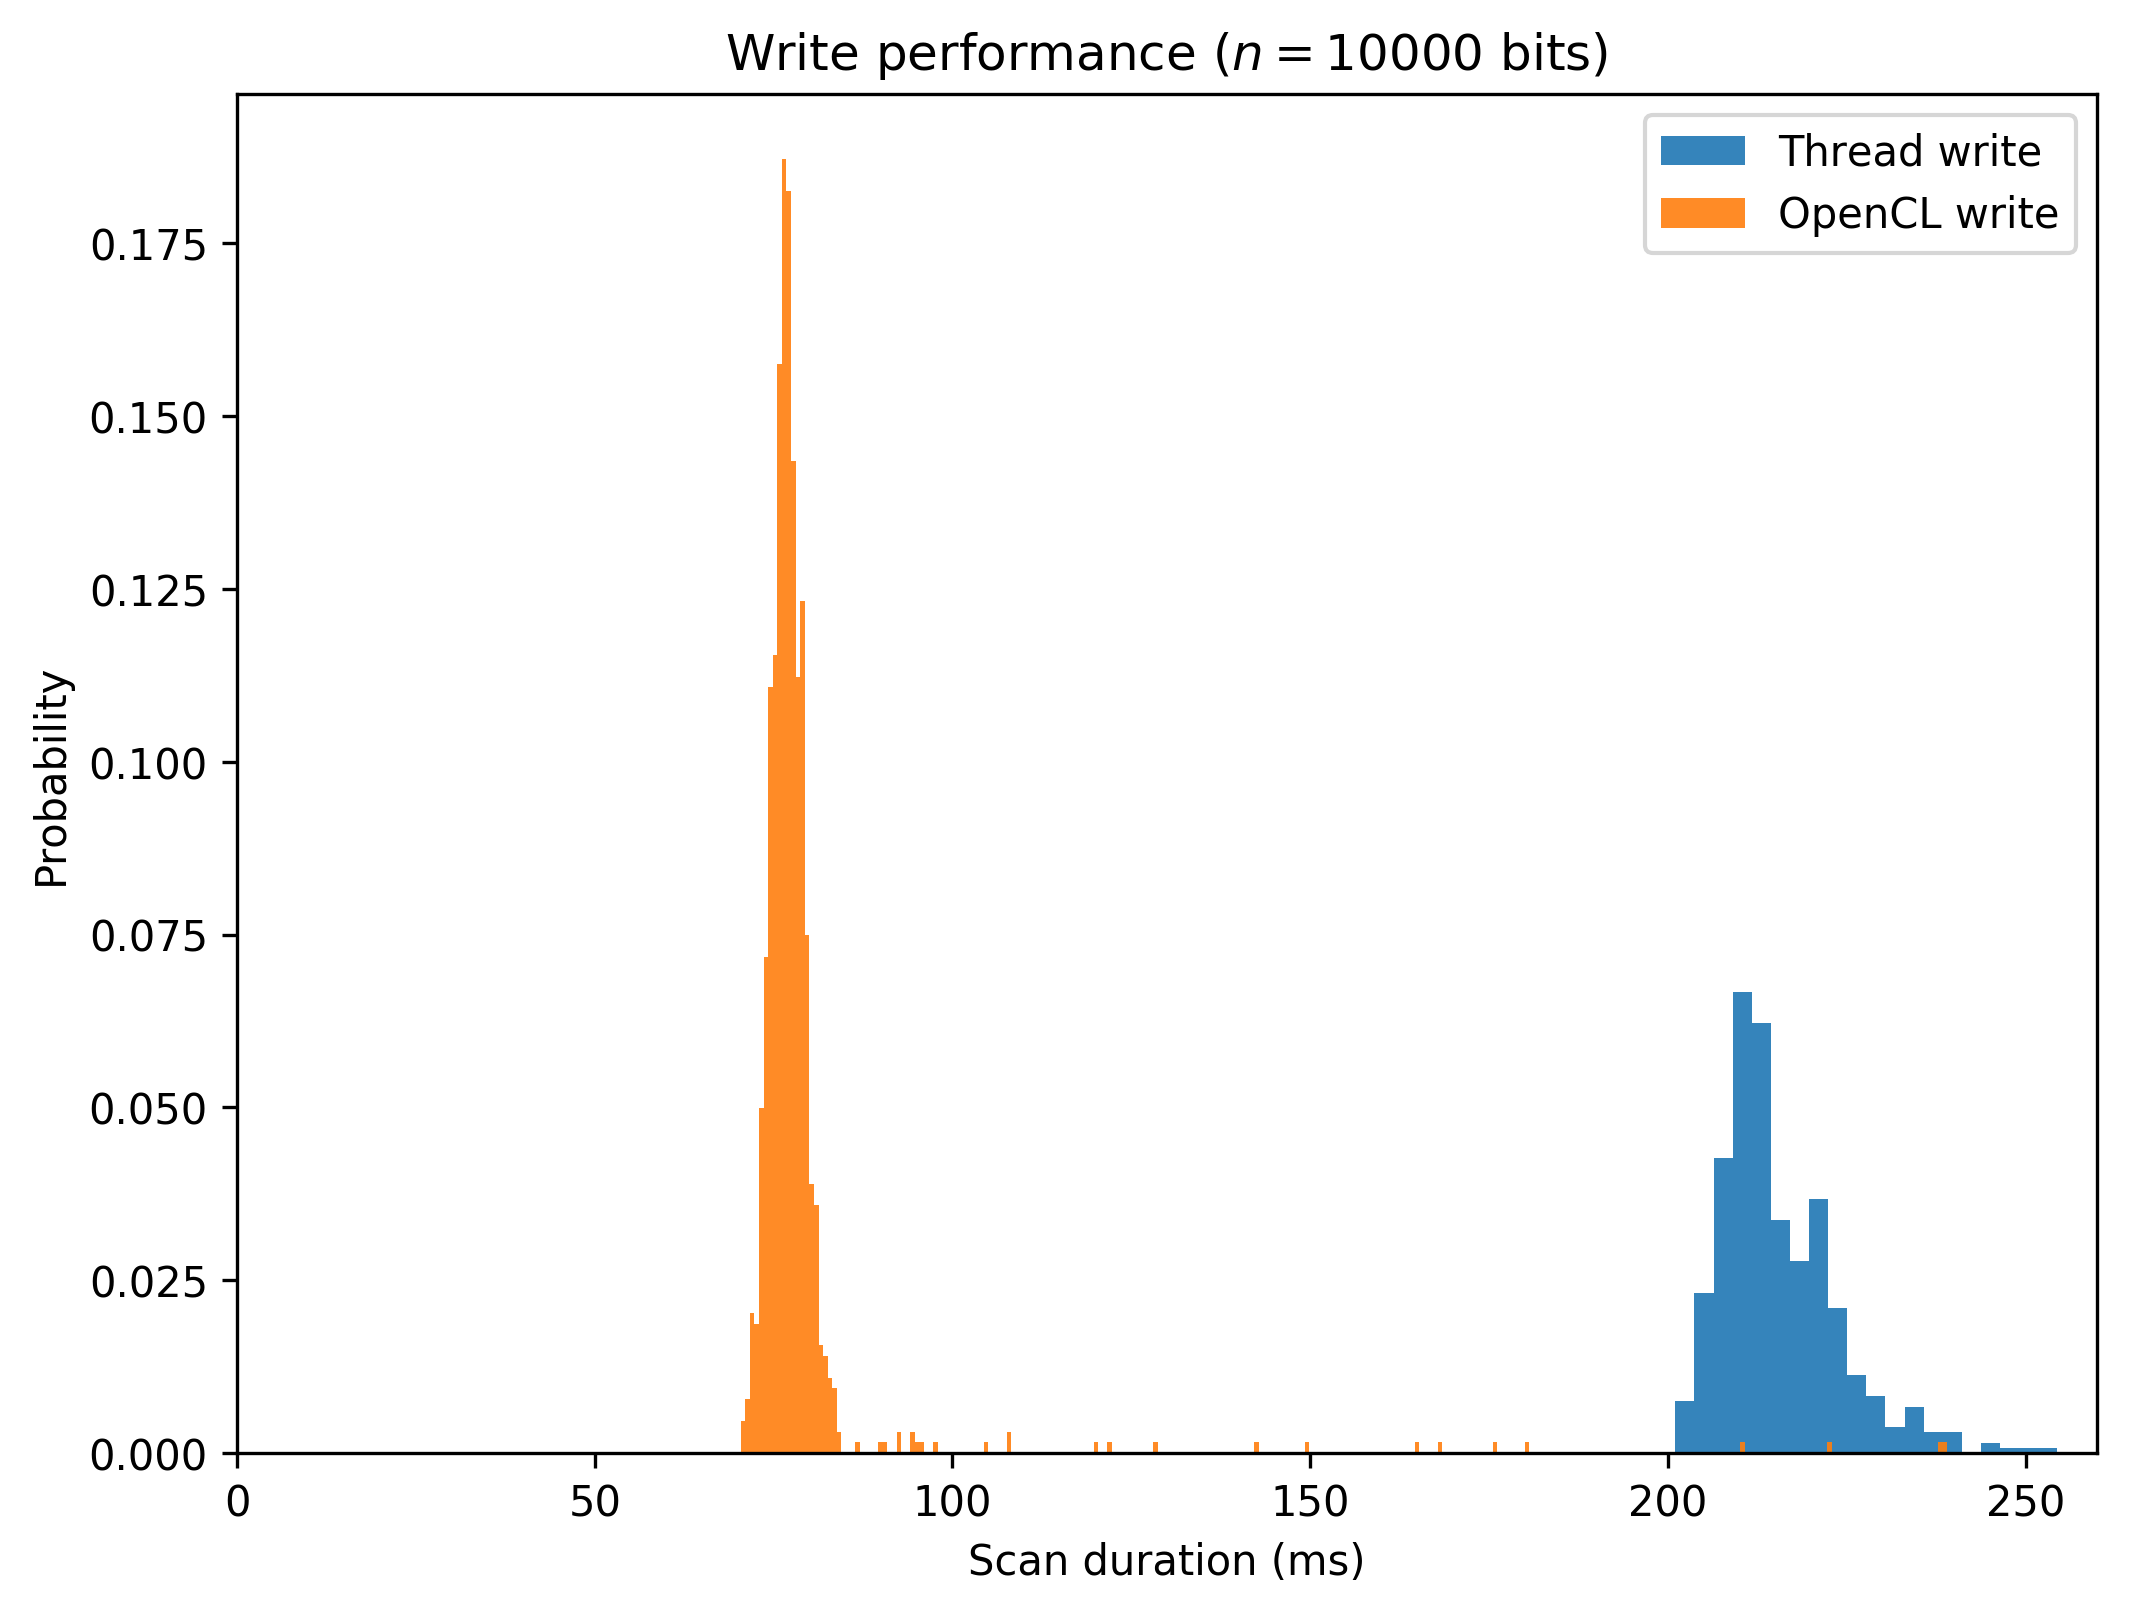
\includegraphics[width=0.7\textwidth]{images02/performance/ec2-p3-write-10k.png}}

\caption{Write operation comparisons for Amazon EC2 p3.2xlarge with Intel Xeon E5-2686v4 processor, 488GB DDR3 RAM, and NVIDIA Tesla V100 GPU.
\label{fig:perf-ec2-p3-write}}
\end{figure}

\subsection{Summary of results}

The results, beyond showing the obvious fact that consumer grade hardware is not comparable to the Amazon instances, indicate a non-trivial issue:  The chosen kernel for scanning the memory is of crucial importance to performance, and this kernel speed is a function of both the hardware used and the particular parameters used in the SDM settings.

It is reasonable to consider that the performance results obtained are of particular merit, and one particular fact stands out:  The scanning of 1,000,000 hard locations has become, in the desired professional-grade machines, \emph{faster} than the updating of the 1,000 active locations.
